\documentclass[twoside]{book}

% Packages required by doxygen
\usepackage{fixltx2e}
\usepackage{calc}
\usepackage{doxygen}
\usepackage[export]{adjustbox} % also loads graphicx
\usepackage{graphicx}
\usepackage[utf8]{inputenc}
\usepackage{makeidx}
\usepackage{multicol}
\usepackage{multirow}
\PassOptionsToPackage{warn}{textcomp}
\usepackage{textcomp}
\usepackage[nointegrals]{wasysym}
\usepackage[table]{xcolor}

% Font selection
\usepackage[T1]{fontenc}
\usepackage[scaled=.90]{helvet}
\usepackage{courier}
\usepackage{amssymb}
\usepackage{sectsty}
\renewcommand{\familydefault}{\sfdefault}
\allsectionsfont{%
  \fontseries{bc}\selectfont%
  \color{darkgray}%
}
\renewcommand{\DoxyLabelFont}{%
  \fontseries{bc}\selectfont%
  \color{darkgray}%
}
\newcommand{\+}{\discretionary{\mbox{\scriptsize$\hookleftarrow$}}{}{}}

% Page & text layout
\usepackage{geometry}
\geometry{%
  a4paper,%
  top=2.5cm,%
  bottom=2.5cm,%
  left=2.5cm,%
  right=2.5cm%
}
\tolerance=750
\hfuzz=15pt
\hbadness=750
\setlength{\emergencystretch}{15pt}
\setlength{\parindent}{0cm}
\setlength{\parskip}{3ex plus 2ex minus 2ex}
\makeatletter
\renewcommand{\paragraph}{%
  \@startsection{paragraph}{4}{0ex}{-1.0ex}{1.0ex}{%
    \normalfont\normalsize\bfseries\SS@parafont%
  }%
}
\renewcommand{\subparagraph}{%
  \@startsection{subparagraph}{5}{0ex}{-1.0ex}{1.0ex}{%
    \normalfont\normalsize\bfseries\SS@subparafont%
  }%
}
\makeatother

% Headers & footers
\usepackage{fancyhdr}
\pagestyle{fancyplain}
\fancyhead[LE]{\fancyplain{}{\bfseries\thepage}}
\fancyhead[CE]{\fancyplain{}{}}
\fancyhead[RE]{\fancyplain{}{\bfseries\leftmark}}
\fancyhead[LO]{\fancyplain{}{\bfseries\rightmark}}
\fancyhead[CO]{\fancyplain{}{}}
\fancyhead[RO]{\fancyplain{}{\bfseries\thepage}}
\fancyfoot[LE]{\fancyplain{}{}}
\fancyfoot[CE]{\fancyplain{}{}}
\fancyfoot[RE]{\fancyplain{}{\bfseries\scriptsize Generated by Doxygen }}
\fancyfoot[LO]{\fancyplain{}{\bfseries\scriptsize Generated by Doxygen }}
\fancyfoot[CO]{\fancyplain{}{}}
\fancyfoot[RO]{\fancyplain{}{}}
\renewcommand{\footrulewidth}{0.4pt}
\renewcommand{\chaptermark}[1]{%
  \markboth{#1}{}%
}
\renewcommand{\sectionmark}[1]{%
  \markright{\thesection\ #1}%
}

% Indices & bibliography
\usepackage{natbib}
\usepackage[titles]{tocloft}
\setcounter{tocdepth}{3}
\setcounter{secnumdepth}{5}
\makeindex

% Hyperlinks (required, but should be loaded last)
\usepackage{ifpdf}
\ifpdf
  \usepackage[pdftex,pagebackref=true]{hyperref}
\else
  \usepackage[ps2pdf,pagebackref=true]{hyperref}
\fi
\hypersetup{%
  colorlinks=true,%
  linkcolor=blue,%
  citecolor=blue,%
  unicode%
}

% Custom commands
\newcommand{\clearemptydoublepage}{%
  \newpage{\pagestyle{empty}\cleardoublepage}%
}

\usepackage{caption}
\captionsetup{labelsep=space,justification=centering,font={bf},singlelinecheck=off,skip=4pt,position=top}

%===== C O N T E N T S =====

\begin{document}

% Titlepage & ToC
\hypersetup{pageanchor=false,
             bookmarksnumbered=true,
             pdfencoding=unicode
            }
\pagenumbering{alph}
\begin{titlepage}
\vspace*{7cm}
\begin{center}%
{\Large cpp\+\_\+redis \\[1ex]\large 4.\+0.\+0 }\\
\vspace*{1cm}
{\large Generated by Doxygen 1.8.13}\\
\end{center}
\end{titlepage}
\clearemptydoublepage
\pagenumbering{roman}
\tableofcontents
\clearemptydoublepage
\pagenumbering{arabic}
\hypersetup{pageanchor=true}

%--- Begin generated contents ---
\chapter{Hierarchical Index}
\section{Class Hierarchy}
This inheritance list is sorted roughly, but not completely, alphabetically\+:\begin{DoxyCompactList}
\item \contentsline{section}{cpp\+\_\+redis\+:\+:helpers\+:\+:back$<$ T, Args $>$}{\pageref{structcpp__redis_1_1helpers_1_1back}}{}
\item \contentsline{section}{cpp\+\_\+redis\+:\+:helpers\+:\+:back$<$ T $>$}{\pageref{structcpp__redis_1_1helpers_1_1back_3_01_t_01_4}}{}
\item \contentsline{section}{cpp\+\_\+redis\+:\+:builders\+:\+:builder\+\_\+iface}{\pageref{classcpp__redis_1_1builders_1_1builder__iface}}{}
\begin{DoxyCompactList}
\item \contentsline{section}{cpp\+\_\+redis\+:\+:builders\+:\+:array\+\_\+builder}{\pageref{classcpp__redis_1_1builders_1_1array__builder}}{}
\item \contentsline{section}{cpp\+\_\+redis\+:\+:builders\+:\+:bulk\+\_\+string\+\_\+builder}{\pageref{classcpp__redis_1_1builders_1_1bulk__string__builder}}{}
\item \contentsline{section}{cpp\+\_\+redis\+:\+:builders\+:\+:error\+\_\+builder}{\pageref{classcpp__redis_1_1builders_1_1error__builder}}{}
\item \contentsline{section}{cpp\+\_\+redis\+:\+:builders\+:\+:integer\+\_\+builder}{\pageref{classcpp__redis_1_1builders_1_1integer__builder}}{}
\item \contentsline{section}{cpp\+\_\+redis\+:\+:builders\+:\+:simple\+\_\+string\+\_\+builder}{\pageref{classcpp__redis_1_1builders_1_1simple__string__builder}}{}
\end{DoxyCompactList}
\item \contentsline{section}{cpp\+\_\+redis\+:\+:subscriber\+:\+:callback\+\_\+holder}{\pageref{structcpp__redis_1_1subscriber_1_1callback__holder}}{}
\item \contentsline{section}{cpp\+\_\+redis\+:\+:client}{\pageref{classcpp__redis_1_1client}}{}
\item \contentsline{section}{cpp\+\_\+redis\+:\+:client\+:\+:command\+\_\+request}{\pageref{structcpp__redis_1_1client_1_1command__request}}{}
\item \contentsline{section}{cpp\+\_\+redis\+:\+:helpers\+:\+:front$<$ T, Ts $>$}{\pageref{structcpp__redis_1_1helpers_1_1front}}{}
\item \contentsline{section}{cpp\+\_\+redis\+:\+:helpers\+:\+:is\+\_\+different\+\_\+types$<$ T, Args $>$}{\pageref{structcpp__redis_1_1helpers_1_1is__different__types}}{}
\item \contentsline{section}{cpp\+\_\+redis\+:\+:helpers\+:\+:is\+\_\+different\+\_\+types$<$ T1 $>$}{\pageref{structcpp__redis_1_1helpers_1_1is__different__types_3_01_t1_01_4}}{}
\item \contentsline{section}{cpp\+\_\+redis\+:\+:helpers\+:\+:is\+\_\+type\+\_\+present$<$ T1, T2, Ts $>$}{\pageref{structcpp__redis_1_1helpers_1_1is__type__present}}{}
\item \contentsline{section}{cpp\+\_\+redis\+:\+:helpers\+:\+:is\+\_\+type\+\_\+present$<$ T1, T2 $>$}{\pageref{structcpp__redis_1_1helpers_1_1is__type__present_3_01_t1_00_01_t2_01_4}}{}
\item \contentsline{section}{cpp\+\_\+redis\+:\+:logger\+\_\+iface}{\pageref{classcpp__redis_1_1logger__iface}}{}
\begin{DoxyCompactList}
\item \contentsline{section}{cpp\+\_\+redis\+:\+:logger}{\pageref{classcpp__redis_1_1logger}}{}
\end{DoxyCompactList}
\item \contentsline{section}{cpp\+\_\+redis\+:\+:network\+:\+:tcp\+\_\+client\+\_\+iface\+:\+:read\+\_\+request}{\pageref{structcpp__redis_1_1network_1_1tcp__client__iface_1_1read__request}}{}
\item \contentsline{section}{cpp\+\_\+redis\+:\+:network\+:\+:tcp\+\_\+client\+\_\+iface\+:\+:read\+\_\+result}{\pageref{structcpp__redis_1_1network_1_1tcp__client__iface_1_1read__result}}{}
\item \contentsline{section}{cpp\+\_\+redis\+:\+:network\+:\+:redis\+\_\+connection}{\pageref{classcpp__redis_1_1network_1_1redis__connection}}{}
\item \contentsline{section}{cpp\+\_\+redis\+:\+:reply}{\pageref{classcpp__redis_1_1reply}}{}
\item \contentsline{section}{cpp\+\_\+redis\+:\+:builders\+:\+:reply\+\_\+builder}{\pageref{classcpp__redis_1_1builders_1_1reply__builder}}{}
\item runtime\+\_\+error\begin{DoxyCompactList}
\item \contentsline{section}{cpp\+\_\+redis\+:\+:redis\+\_\+error}{\pageref{classcpp__redis_1_1redis__error}}{}
\end{DoxyCompactList}
\item \contentsline{section}{cpp\+\_\+redis\+:\+:sentinel}{\pageref{classcpp__redis_1_1sentinel}}{}
\item \contentsline{section}{cpp\+\_\+redis\+:\+:sentinel\+:\+:sentinel\+\_\+def}{\pageref{classcpp__redis_1_1sentinel_1_1sentinel__def}}{}
\item \contentsline{section}{cpp\+\_\+redis\+:\+:subscriber}{\pageref{classcpp__redis_1_1subscriber}}{}
\item \contentsline{section}{cpp\+\_\+redis\+:\+:network\+:\+:tcp\+\_\+client\+\_\+iface}{\pageref{classcpp__redis_1_1network_1_1tcp__client__iface}}{}
\begin{DoxyCompactList}
\item \contentsline{section}{cpp\+\_\+redis\+:\+:network\+:\+:tcp\+\_\+client}{\pageref{classcpp__redis_1_1network_1_1tcp__client}}{}
\end{DoxyCompactList}
\item \contentsline{section}{cpp\+\_\+redis\+:\+:network\+:\+:tcp\+\_\+client\+\_\+iface\+:\+:write\+\_\+request}{\pageref{structcpp__redis_1_1network_1_1tcp__client__iface_1_1write__request}}{}
\item \contentsline{section}{cpp\+\_\+redis\+:\+:network\+:\+:tcp\+\_\+client\+\_\+iface\+:\+:write\+\_\+result}{\pageref{structcpp__redis_1_1network_1_1tcp__client__iface_1_1write__result}}{}
\end{DoxyCompactList}

\chapter{Class Index}
\section{Class List}
Here are the classes, structs, unions and interfaces with brief descriptions\+:\begin{DoxyCompactList}
\item\contentsline{section}{\hyperlink{classcpp__redis_1_1builders_1_1array__builder}{cpp\+\_\+redis\+::builders\+::array\+\_\+builder} }{\pageref{classcpp__redis_1_1builders_1_1array__builder}}{}
\item\contentsline{section}{\hyperlink{structcpp__redis_1_1helpers_1_1back}{cpp\+\_\+redis\+::helpers\+::back$<$ T, Args $>$} }{\pageref{structcpp__redis_1_1helpers_1_1back}}{}
\item\contentsline{section}{\hyperlink{structcpp__redis_1_1helpers_1_1back_3_01_t_01_4}{cpp\+\_\+redis\+::helpers\+::back$<$ T $>$} }{\pageref{structcpp__redis_1_1helpers_1_1back_3_01_t_01_4}}{}
\item\contentsline{section}{\hyperlink{structcpp__redis_1_1client_1_1bitfield__operation}{cpp\+\_\+redis\+::client\+::bitfield\+\_\+operation} }{\pageref{structcpp__redis_1_1client_1_1bitfield__operation}}{}
\item\contentsline{section}{\hyperlink{classcpp__redis_1_1builders_1_1builder__iface}{cpp\+\_\+redis\+::builders\+::builder\+\_\+iface} }{\pageref{classcpp__redis_1_1builders_1_1builder__iface}}{}
\item\contentsline{section}{\hyperlink{classcpp__redis_1_1builders_1_1bulk__string__builder}{cpp\+\_\+redis\+::builders\+::bulk\+\_\+string\+\_\+builder} }{\pageref{classcpp__redis_1_1builders_1_1bulk__string__builder}}{}
\item\contentsline{section}{\hyperlink{classcpp__redis_1_1client}{cpp\+\_\+redis\+::client} }{\pageref{classcpp__redis_1_1client}}{}
\item\contentsline{section}{\hyperlink{classcpp__redis_1_1builders_1_1error__builder}{cpp\+\_\+redis\+::builders\+::error\+\_\+builder} }{\pageref{classcpp__redis_1_1builders_1_1error__builder}}{}
\item\contentsline{section}{\hyperlink{structcpp__redis_1_1helpers_1_1front}{cpp\+\_\+redis\+::helpers\+::front$<$ T, Ts $>$} }{\pageref{structcpp__redis_1_1helpers_1_1front}}{}
\item\contentsline{section}{\hyperlink{classcpp__redis_1_1builders_1_1integer__builder}{cpp\+\_\+redis\+::builders\+::integer\+\_\+builder} }{\pageref{classcpp__redis_1_1builders_1_1integer__builder}}{}
\item\contentsline{section}{\hyperlink{structcpp__redis_1_1helpers_1_1is__different__types}{cpp\+\_\+redis\+::helpers\+::is\+\_\+different\+\_\+types$<$ T, Args $>$} }{\pageref{structcpp__redis_1_1helpers_1_1is__different__types}}{}
\item\contentsline{section}{\hyperlink{structcpp__redis_1_1helpers_1_1is__different__types_3_01_t1_01_4}{cpp\+\_\+redis\+::helpers\+::is\+\_\+different\+\_\+types$<$ T1 $>$} }{\pageref{structcpp__redis_1_1helpers_1_1is__different__types_3_01_t1_01_4}}{}
\item\contentsline{section}{\hyperlink{structcpp__redis_1_1helpers_1_1is__type__present}{cpp\+\_\+redis\+::helpers\+::is\+\_\+type\+\_\+present$<$ T1, T2, Ts $>$} }{\pageref{structcpp__redis_1_1helpers_1_1is__type__present}}{}
\item\contentsline{section}{\hyperlink{structcpp__redis_1_1helpers_1_1is__type__present_3_01_t1_00_01_t2_01_4}{cpp\+\_\+redis\+::helpers\+::is\+\_\+type\+\_\+present$<$ T1, T2 $>$} }{\pageref{structcpp__redis_1_1helpers_1_1is__type__present_3_01_t1_00_01_t2_01_4}}{}
\item\contentsline{section}{\hyperlink{classcpp__redis_1_1logger}{cpp\+\_\+redis\+::logger} }{\pageref{classcpp__redis_1_1logger}}{}
\item\contentsline{section}{\hyperlink{classcpp__redis_1_1logger__iface}{cpp\+\_\+redis\+::logger\+\_\+iface} }{\pageref{classcpp__redis_1_1logger__iface}}{}
\item\contentsline{section}{\hyperlink{structcpp__redis_1_1network_1_1tcp__client__iface_1_1read__request}{cpp\+\_\+redis\+::network\+::tcp\+\_\+client\+\_\+iface\+::read\+\_\+request} }{\pageref{structcpp__redis_1_1network_1_1tcp__client__iface_1_1read__request}}{}
\item\contentsline{section}{\hyperlink{structcpp__redis_1_1network_1_1tcp__client__iface_1_1read__result}{cpp\+\_\+redis\+::network\+::tcp\+\_\+client\+\_\+iface\+::read\+\_\+result} }{\pageref{structcpp__redis_1_1network_1_1tcp__client__iface_1_1read__result}}{}
\item\contentsline{section}{\hyperlink{classcpp__redis_1_1network_1_1redis__connection}{cpp\+\_\+redis\+::network\+::redis\+\_\+connection} }{\pageref{classcpp__redis_1_1network_1_1redis__connection}}{}
\item\contentsline{section}{\hyperlink{classcpp__redis_1_1redis__error}{cpp\+\_\+redis\+::redis\+\_\+error} }{\pageref{classcpp__redis_1_1redis__error}}{}
\item\contentsline{section}{\hyperlink{classcpp__redis_1_1reply}{cpp\+\_\+redis\+::reply} }{\pageref{classcpp__redis_1_1reply}}{}
\item\contentsline{section}{\hyperlink{classcpp__redis_1_1builders_1_1reply__builder}{cpp\+\_\+redis\+::builders\+::reply\+\_\+builder} }{\pageref{classcpp__redis_1_1builders_1_1reply__builder}}{}
\item\contentsline{section}{\hyperlink{classcpp__redis_1_1sentinel}{cpp\+\_\+redis\+::sentinel} }{\pageref{classcpp__redis_1_1sentinel}}{}
\item\contentsline{section}{\hyperlink{classcpp__redis_1_1builders_1_1simple__string__builder}{cpp\+\_\+redis\+::builders\+::simple\+\_\+string\+\_\+builder} }{\pageref{classcpp__redis_1_1builders_1_1simple__string__builder}}{}
\item\contentsline{section}{\hyperlink{classcpp__redis_1_1subscriber}{cpp\+\_\+redis\+::subscriber} }{\pageref{classcpp__redis_1_1subscriber}}{}
\item\contentsline{section}{\hyperlink{classcpp__redis_1_1network_1_1tcp__client}{cpp\+\_\+redis\+::network\+::tcp\+\_\+client} }{\pageref{classcpp__redis_1_1network_1_1tcp__client}}{}
\item\contentsline{section}{\hyperlink{classcpp__redis_1_1network_1_1tcp__client__iface}{cpp\+\_\+redis\+::network\+::tcp\+\_\+client\+\_\+iface} }{\pageref{classcpp__redis_1_1network_1_1tcp__client__iface}}{}
\item\contentsline{section}{\hyperlink{structcpp__redis_1_1network_1_1tcp__client__iface_1_1write__request}{cpp\+\_\+redis\+::network\+::tcp\+\_\+client\+\_\+iface\+::write\+\_\+request} }{\pageref{structcpp__redis_1_1network_1_1tcp__client__iface_1_1write__request}}{}
\item\contentsline{section}{\hyperlink{structcpp__redis_1_1network_1_1tcp__client__iface_1_1write__result}{cpp\+\_\+redis\+::network\+::tcp\+\_\+client\+\_\+iface\+::write\+\_\+result} }{\pageref{structcpp__redis_1_1network_1_1tcp__client__iface_1_1write__result}}{}
\end{DoxyCompactList}

\chapter{Class Documentation}
\hypertarget{classcpp__redis_1_1builders_1_1array__builder}{}\section{cpp\+\_\+redis\+:\+:builders\+:\+:array\+\_\+builder Class Reference}
\label{classcpp__redis_1_1builders_1_1array__builder}\index{cpp\+\_\+redis\+::builders\+::array\+\_\+builder@{cpp\+\_\+redis\+::builders\+::array\+\_\+builder}}


{\ttfamily \#include $<$array\+\_\+builder.\+hpp$>$}

Inheritance diagram for cpp\+\_\+redis\+:\+:builders\+:\+:array\+\_\+builder\+:\begin{figure}[H]
\begin{center}
\leavevmode
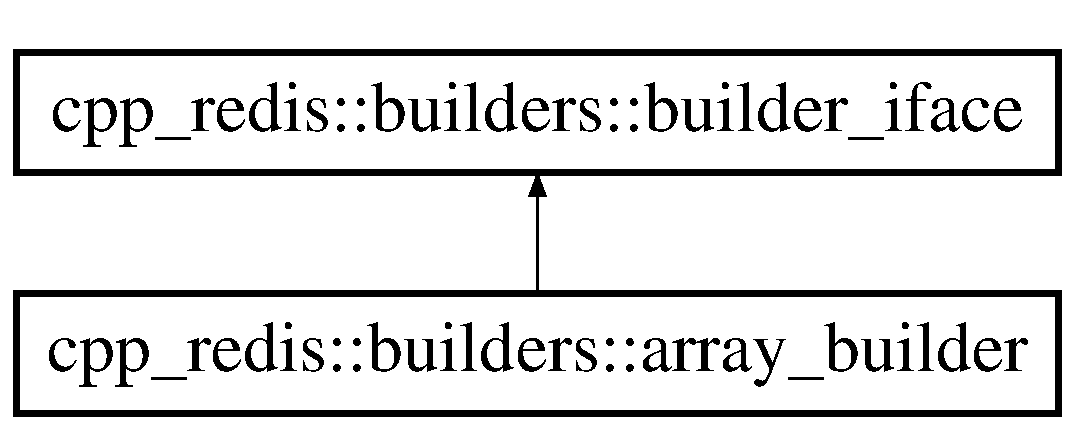
\includegraphics[height=2.000000cm]{classcpp__redis_1_1builders_1_1array__builder}
\end{center}
\end{figure}
\subsection*{Public Member Functions}
\begin{DoxyCompactItemize}
\item 
\mbox{\Hypertarget{classcpp__redis_1_1builders_1_1array__builder_a4beae33a547d3d7efc112659411a23a3}\label{classcpp__redis_1_1builders_1_1array__builder_a4beae33a547d3d7efc112659411a23a3}} 
\hyperlink{classcpp__redis_1_1builders_1_1array__builder_a4beae33a547d3d7efc112659411a23a3}{array\+\_\+builder} (void)
\begin{DoxyCompactList}\small\item\em ctor \end{DoxyCompactList}\item 
\mbox{\Hypertarget{classcpp__redis_1_1builders_1_1array__builder_ae6a0cd0743b6b0a21f9c3d44fd31ac17}\label{classcpp__redis_1_1builders_1_1array__builder_ae6a0cd0743b6b0a21f9c3d44fd31ac17}} 
\hyperlink{classcpp__redis_1_1builders_1_1array__builder_ae6a0cd0743b6b0a21f9c3d44fd31ac17}{$\sim$array\+\_\+builder} (void)=default
\begin{DoxyCompactList}\small\item\em dtor \end{DoxyCompactList}\item 
\mbox{\Hypertarget{classcpp__redis_1_1builders_1_1array__builder_aa0e5fe9a587b277a473d66b7e6db9548}\label{classcpp__redis_1_1builders_1_1array__builder_aa0e5fe9a587b277a473d66b7e6db9548}} 
\hyperlink{classcpp__redis_1_1builders_1_1array__builder_aa0e5fe9a587b277a473d66b7e6db9548}{array\+\_\+builder} (const \hyperlink{classcpp__redis_1_1builders_1_1array__builder}{array\+\_\+builder} \&)=delete
\begin{DoxyCompactList}\small\item\em copy ctor \end{DoxyCompactList}\item 
\mbox{\Hypertarget{classcpp__redis_1_1builders_1_1array__builder_aaa1df845df7a007cf73f95f73e800c2c}\label{classcpp__redis_1_1builders_1_1array__builder_aaa1df845df7a007cf73f95f73e800c2c}} 
\hyperlink{classcpp__redis_1_1builders_1_1array__builder}{array\+\_\+builder} \& \hyperlink{classcpp__redis_1_1builders_1_1array__builder_aaa1df845df7a007cf73f95f73e800c2c}{operator=} (const \hyperlink{classcpp__redis_1_1builders_1_1array__builder}{array\+\_\+builder} \&)=delete
\begin{DoxyCompactList}\small\item\em assignment operator \end{DoxyCompactList}\item 
\hyperlink{classcpp__redis_1_1builders_1_1builder__iface}{builder\+\_\+iface} \& \hyperlink{classcpp__redis_1_1builders_1_1array__builder_a043357d0ef70406adef4df78c8d5307f}{operator$<$$<$} (std\+::string \&data)
\item 
bool \hyperlink{classcpp__redis_1_1builders_1_1array__builder_a524f2cb943dde1246dea1b7057e6351e}{reply\+\_\+ready} (void) const
\item 
\hyperlink{classcpp__redis_1_1reply}{reply} \hyperlink{classcpp__redis_1_1builders_1_1array__builder_ac5c805ad87b357a9578c5a0d479109b3}{get\+\_\+reply} (void) const
\end{DoxyCompactItemize}


\subsection{Detailed Description}
builder to build redis array replies 

\subsection{Member Function Documentation}
\mbox{\Hypertarget{classcpp__redis_1_1builders_1_1array__builder_ac5c805ad87b357a9578c5a0d479109b3}\label{classcpp__redis_1_1builders_1_1array__builder_ac5c805ad87b357a9578c5a0d479109b3}} 
\index{cpp\+\_\+redis\+::builders\+::array\+\_\+builder@{cpp\+\_\+redis\+::builders\+::array\+\_\+builder}!get\+\_\+reply@{get\+\_\+reply}}
\index{get\+\_\+reply@{get\+\_\+reply}!cpp\+\_\+redis\+::builders\+::array\+\_\+builder@{cpp\+\_\+redis\+::builders\+::array\+\_\+builder}}
\subsubsection{\texorpdfstring{get\+\_\+reply()}{get\_reply()}}
{\footnotesize\ttfamily \hyperlink{classcpp__redis_1_1reply}{reply} cpp\+\_\+redis\+::builders\+::array\+\_\+builder\+::get\+\_\+reply (\begin{DoxyParamCaption}\item[{void}]{ }\end{DoxyParamCaption}) const\hspace{0.3cm}{\ttfamily [virtual]}}

\begin{DoxyReturn}{Returns}
reply object 
\end{DoxyReturn}


Implements \hyperlink{classcpp__redis_1_1builders_1_1builder__iface_afd2ff2c2371c2a486116543b638b9413}{cpp\+\_\+redis\+::builders\+::builder\+\_\+iface}.

\mbox{\Hypertarget{classcpp__redis_1_1builders_1_1array__builder_a043357d0ef70406adef4df78c8d5307f}\label{classcpp__redis_1_1builders_1_1array__builder_a043357d0ef70406adef4df78c8d5307f}} 
\index{cpp\+\_\+redis\+::builders\+::array\+\_\+builder@{cpp\+\_\+redis\+::builders\+::array\+\_\+builder}!operator$<$$<$@{operator$<$$<$}}
\index{operator$<$$<$@{operator$<$$<$}!cpp\+\_\+redis\+::builders\+::array\+\_\+builder@{cpp\+\_\+redis\+::builders\+::array\+\_\+builder}}
\subsubsection{\texorpdfstring{operator$<$$<$()}{operator<<()}}
{\footnotesize\ttfamily \hyperlink{classcpp__redis_1_1builders_1_1builder__iface}{builder\+\_\+iface}\& cpp\+\_\+redis\+::builders\+::array\+\_\+builder\+::operator$<$$<$ (\begin{DoxyParamCaption}\item[{std\+::string \&}]{data }\end{DoxyParamCaption})\hspace{0.3cm}{\ttfamily [virtual]}}

take data as parameter which is consumed to build the reply every bytes used to build the reply must be removed from the buffer passed as parameter


\begin{DoxyParams}{Parameters}
{\em data} & data to be consumed \\
\hline
\end{DoxyParams}
\begin{DoxyReturn}{Returns}
current instance 
\end{DoxyReturn}


Implements \hyperlink{classcpp__redis_1_1builders_1_1builder__iface_a9892bbc9c887c31c2742dad4476e2fa6}{cpp\+\_\+redis\+::builders\+::builder\+\_\+iface}.

\mbox{\Hypertarget{classcpp__redis_1_1builders_1_1array__builder_a524f2cb943dde1246dea1b7057e6351e}\label{classcpp__redis_1_1builders_1_1array__builder_a524f2cb943dde1246dea1b7057e6351e}} 
\index{cpp\+\_\+redis\+::builders\+::array\+\_\+builder@{cpp\+\_\+redis\+::builders\+::array\+\_\+builder}!reply\+\_\+ready@{reply\+\_\+ready}}
\index{reply\+\_\+ready@{reply\+\_\+ready}!cpp\+\_\+redis\+::builders\+::array\+\_\+builder@{cpp\+\_\+redis\+::builders\+::array\+\_\+builder}}
\subsubsection{\texorpdfstring{reply\+\_\+ready()}{reply\_ready()}}
{\footnotesize\ttfamily bool cpp\+\_\+redis\+::builders\+::array\+\_\+builder\+::reply\+\_\+ready (\begin{DoxyParamCaption}\item[{void}]{ }\end{DoxyParamCaption}) const\hspace{0.3cm}{\ttfamily [virtual]}}

\begin{DoxyReturn}{Returns}
whether the reply could be built 
\end{DoxyReturn}


Implements \hyperlink{classcpp__redis_1_1builders_1_1builder__iface_a40db9a31d4ea1771777e74146d31e12d}{cpp\+\_\+redis\+::builders\+::builder\+\_\+iface}.



The documentation for this class was generated from the following file\+:\begin{DoxyCompactItemize}
\item 
includes/cpp\+\_\+redis/builders/array\+\_\+builder.\+hpp\end{DoxyCompactItemize}

\hypertarget{structcpp__redis_1_1helpers_1_1back}{}\section{cpp\+\_\+redis\+:\+:helpers\+:\+:back$<$ T, Args $>$ Struct Template Reference}
\label{structcpp__redis_1_1helpers_1_1back}\index{cpp\+\_\+redis\+::helpers\+::back$<$ T, Args $>$@{cpp\+\_\+redis\+::helpers\+::back$<$ T, Args $>$}}


{\ttfamily \#include $<$variadic\+\_\+template.\+hpp$>$}

\subsection*{Public Types}
\begin{DoxyCompactItemize}
\item 
using \hyperlink{structcpp__redis_1_1helpers_1_1back_a83f1d0c03ffc82ff8ab7243c3c858195}{type} = typename \hyperlink{structcpp__redis_1_1helpers_1_1back}{back}$<$ Args... $>$\+::\hyperlink{structcpp__redis_1_1helpers_1_1back_a83f1d0c03ffc82ff8ab7243c3c858195}{type}
\end{DoxyCompactItemize}


\subsection{Detailed Description}
\subsubsection*{template$<$typename T, typename... Args$>$\newline
struct cpp\+\_\+redis\+::helpers\+::back$<$ T, Args $>$}

type traits to return last element of a variadic list 

\subsection{Member Typedef Documentation}
\mbox{\Hypertarget{structcpp__redis_1_1helpers_1_1back_a83f1d0c03ffc82ff8ab7243c3c858195}\label{structcpp__redis_1_1helpers_1_1back_a83f1d0c03ffc82ff8ab7243c3c858195}} 
\index{cpp\+\_\+redis\+::helpers\+::back@{cpp\+\_\+redis\+::helpers\+::back}!type@{type}}
\index{type@{type}!cpp\+\_\+redis\+::helpers\+::back@{cpp\+\_\+redis\+::helpers\+::back}}
\subsubsection{\texorpdfstring{type}{type}}
{\footnotesize\ttfamily template$<$typename T , typename... Args$>$ \\
using \hyperlink{structcpp__redis_1_1helpers_1_1back}{cpp\+\_\+redis\+::helpers\+::back}$<$ T, Args $>$\+::\hyperlink{structcpp__redis_1_1helpers_1_1back_a83f1d0c03ffc82ff8ab7243c3c858195}{type} =  typename \hyperlink{structcpp__redis_1_1helpers_1_1back}{back}$<$Args...$>$\+::\hyperlink{structcpp__redis_1_1helpers_1_1back_a83f1d0c03ffc82ff8ab7243c3c858195}{type}}

last type of variadic list 

The documentation for this struct was generated from the following file\+:\begin{DoxyCompactItemize}
\item 
includes/cpp\+\_\+redis/helpers/variadic\+\_\+template.\+hpp\end{DoxyCompactItemize}

\hypertarget{structcpp__redis_1_1helpers_1_1back_3_01_t_01_4}{}\section{cpp\+\_\+redis\+:\+:helpers\+:\+:back$<$ T $>$ Struct Template Reference}
\label{structcpp__redis_1_1helpers_1_1back_3_01_t_01_4}\index{cpp\+\_\+redis\+::helpers\+::back$<$ T $>$@{cpp\+\_\+redis\+::helpers\+::back$<$ T $>$}}


{\ttfamily \#include $<$variadic\+\_\+template.\+hpp$>$}

\subsection*{Public Types}
\begin{DoxyCompactItemize}
\item 
using \hyperlink{structcpp__redis_1_1helpers_1_1back_3_01_t_01_4_a87d10cfacd8ca29b083dc5688e77f87c}{type} = T
\end{DoxyCompactItemize}


\subsection{Detailed Description}
\subsubsection*{template$<$typename T$>$\newline
struct cpp\+\_\+redis\+::helpers\+::back$<$ T $>$}

type traits to return last element of a variadic list 

\subsection{Member Typedef Documentation}
\mbox{\Hypertarget{structcpp__redis_1_1helpers_1_1back_3_01_t_01_4_a87d10cfacd8ca29b083dc5688e77f87c}\label{structcpp__redis_1_1helpers_1_1back_3_01_t_01_4_a87d10cfacd8ca29b083dc5688e77f87c}} 
\index{cpp\+\_\+redis\+::helpers\+::back$<$ T $>$@{cpp\+\_\+redis\+::helpers\+::back$<$ T $>$}!type@{type}}
\index{type@{type}!cpp\+\_\+redis\+::helpers\+::back$<$ T $>$@{cpp\+\_\+redis\+::helpers\+::back$<$ T $>$}}
\subsubsection{\texorpdfstring{type}{type}}
{\footnotesize\ttfamily template$<$typename T $>$ \\
using \hyperlink{structcpp__redis_1_1helpers_1_1back}{cpp\+\_\+redis\+::helpers\+::back}$<$ T $>$\+::\hyperlink{structcpp__redis_1_1helpers_1_1back_3_01_t_01_4_a87d10cfacd8ca29b083dc5688e77f87c}{type} =  T}

templated type 

The documentation for this struct was generated from the following file\+:\begin{DoxyCompactItemize}
\item 
includes/cpp\+\_\+redis/helpers/variadic\+\_\+template.\+hpp\end{DoxyCompactItemize}

\hypertarget{classcpp__redis_1_1builders_1_1builder__iface}{}\section{cpp\+\_\+redis\+:\+:builders\+:\+:builder\+\_\+iface Class Reference}
\label{classcpp__redis_1_1builders_1_1builder__iface}\index{cpp\+\_\+redis\+::builders\+::builder\+\_\+iface@{cpp\+\_\+redis\+::builders\+::builder\+\_\+iface}}


{\ttfamily \#include $<$builder\+\_\+iface.\+hpp$>$}

Inheritance diagram for cpp\+\_\+redis\+:\+:builders\+:\+:builder\+\_\+iface\+:\begin{figure}[H]
\begin{center}
\leavevmode
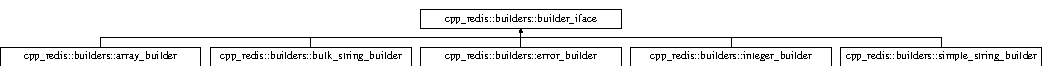
\includegraphics[height=0.888889cm]{classcpp__redis_1_1builders_1_1builder__iface}
\end{center}
\end{figure}
\subsection*{Public Member Functions}
\begin{DoxyCompactItemize}
\item 
virtual \mbox{\hyperlink{classcpp__redis_1_1builders_1_1builder__iface}{builder\+\_\+iface}} \& \mbox{\hyperlink{classcpp__redis_1_1builders_1_1builder__iface_a9892bbc9c887c31c2742dad4476e2fa6}{operator$<$$<$}} (std\+::string \&data)=0
\item 
virtual bool \mbox{\hyperlink{classcpp__redis_1_1builders_1_1builder__iface_a40db9a31d4ea1771777e74146d31e12d}{reply\+\_\+ready}} (void) const =0
\item 
virtual \mbox{\hyperlink{classcpp__redis_1_1reply}{reply}} \mbox{\hyperlink{classcpp__redis_1_1builders_1_1builder__iface_afd2ff2c2371c2a486116543b638b9413}{get\+\_\+reply}} (void) const =0
\end{DoxyCompactItemize}


\subsection{Detailed Description}
interface inherited by all builders 

\subsection{Member Function Documentation}
\mbox{\Hypertarget{classcpp__redis_1_1builders_1_1builder__iface_afd2ff2c2371c2a486116543b638b9413}\label{classcpp__redis_1_1builders_1_1builder__iface_afd2ff2c2371c2a486116543b638b9413}} 
\index{cpp\+\_\+redis\+::builders\+::builder\+\_\+iface@{cpp\+\_\+redis\+::builders\+::builder\+\_\+iface}!get\+\_\+reply@{get\+\_\+reply}}
\index{get\+\_\+reply@{get\+\_\+reply}!cpp\+\_\+redis\+::builders\+::builder\+\_\+iface@{cpp\+\_\+redis\+::builders\+::builder\+\_\+iface}}
\subsubsection{\texorpdfstring{get\+\_\+reply()}{get\_reply()}}
{\footnotesize\ttfamily virtual \mbox{\hyperlink{classcpp__redis_1_1reply}{reply}} cpp\+\_\+redis\+::builders\+::builder\+\_\+iface\+::get\+\_\+reply (\begin{DoxyParamCaption}\item[{void}]{ }\end{DoxyParamCaption}) const\hspace{0.3cm}{\ttfamily [pure virtual]}}

\begin{DoxyReturn}{Returns}
reply object 
\end{DoxyReturn}


Implemented in \mbox{\hyperlink{classcpp__redis_1_1builders_1_1integer__builder_a25221763ba6f8b740458c673945208e0}{cpp\+\_\+redis\+::builders\+::integer\+\_\+builder}}, \mbox{\hyperlink{classcpp__redis_1_1builders_1_1simple__string__builder_a24ad0968d7d02172a65cf8982c540d51}{cpp\+\_\+redis\+::builders\+::simple\+\_\+string\+\_\+builder}}, \mbox{\hyperlink{classcpp__redis_1_1builders_1_1array__builder_ac5c805ad87b357a9578c5a0d479109b3}{cpp\+\_\+redis\+::builders\+::array\+\_\+builder}}, \mbox{\hyperlink{classcpp__redis_1_1builders_1_1bulk__string__builder_a56d6d3089107a1bccd63f6a5267c16cb}{cpp\+\_\+redis\+::builders\+::bulk\+\_\+string\+\_\+builder}}, and \mbox{\hyperlink{classcpp__redis_1_1builders_1_1error__builder_ae2b68b7daad4d71b6780e47bdcc1e32b}{cpp\+\_\+redis\+::builders\+::error\+\_\+builder}}.

\mbox{\Hypertarget{classcpp__redis_1_1builders_1_1builder__iface_a9892bbc9c887c31c2742dad4476e2fa6}\label{classcpp__redis_1_1builders_1_1builder__iface_a9892bbc9c887c31c2742dad4476e2fa6}} 
\index{cpp\+\_\+redis\+::builders\+::builder\+\_\+iface@{cpp\+\_\+redis\+::builders\+::builder\+\_\+iface}!operator$<$$<$@{operator$<$$<$}}
\index{operator$<$$<$@{operator$<$$<$}!cpp\+\_\+redis\+::builders\+::builder\+\_\+iface@{cpp\+\_\+redis\+::builders\+::builder\+\_\+iface}}
\subsubsection{\texorpdfstring{operator$<$$<$()}{operator<<()}}
{\footnotesize\ttfamily virtual \mbox{\hyperlink{classcpp__redis_1_1builders_1_1builder__iface}{builder\+\_\+iface}}\& cpp\+\_\+redis\+::builders\+::builder\+\_\+iface\+::operator$<$$<$ (\begin{DoxyParamCaption}\item[{std\+::string \&}]{data }\end{DoxyParamCaption})\hspace{0.3cm}{\ttfamily [pure virtual]}}

take data as parameter which is consumed to build the reply every bytes used to build the reply must be removed from the buffer passed as parameter


\begin{DoxyParams}{Parameters}
{\em data} & data to be consumed \\
\hline
\end{DoxyParams}
\begin{DoxyReturn}{Returns}
current instance 
\end{DoxyReturn}


Implemented in \mbox{\hyperlink{classcpp__redis_1_1builders_1_1integer__builder_ae29f074134f7269db7f947b0fcbe312e}{cpp\+\_\+redis\+::builders\+::integer\+\_\+builder}}, \mbox{\hyperlink{classcpp__redis_1_1builders_1_1simple__string__builder_a159bb512f0427c4a988742f7cd01035e}{cpp\+\_\+redis\+::builders\+::simple\+\_\+string\+\_\+builder}}, \mbox{\hyperlink{classcpp__redis_1_1builders_1_1array__builder_a043357d0ef70406adef4df78c8d5307f}{cpp\+\_\+redis\+::builders\+::array\+\_\+builder}}, \mbox{\hyperlink{classcpp__redis_1_1builders_1_1bulk__string__builder_a43000357f87212f657aafe279a92b541}{cpp\+\_\+redis\+::builders\+::bulk\+\_\+string\+\_\+builder}}, and \mbox{\hyperlink{classcpp__redis_1_1builders_1_1error__builder_af5ac542be148d6f8500de79fa3164798}{cpp\+\_\+redis\+::builders\+::error\+\_\+builder}}.

\mbox{\Hypertarget{classcpp__redis_1_1builders_1_1builder__iface_a40db9a31d4ea1771777e74146d31e12d}\label{classcpp__redis_1_1builders_1_1builder__iface_a40db9a31d4ea1771777e74146d31e12d}} 
\index{cpp\+\_\+redis\+::builders\+::builder\+\_\+iface@{cpp\+\_\+redis\+::builders\+::builder\+\_\+iface}!reply\+\_\+ready@{reply\+\_\+ready}}
\index{reply\+\_\+ready@{reply\+\_\+ready}!cpp\+\_\+redis\+::builders\+::builder\+\_\+iface@{cpp\+\_\+redis\+::builders\+::builder\+\_\+iface}}
\subsubsection{\texorpdfstring{reply\+\_\+ready()}{reply\_ready()}}
{\footnotesize\ttfamily virtual bool cpp\+\_\+redis\+::builders\+::builder\+\_\+iface\+::reply\+\_\+ready (\begin{DoxyParamCaption}\item[{void}]{ }\end{DoxyParamCaption}) const\hspace{0.3cm}{\ttfamily [pure virtual]}}

\begin{DoxyReturn}{Returns}
whether the reply could be built 
\end{DoxyReturn}


Implemented in \mbox{\hyperlink{classcpp__redis_1_1builders_1_1integer__builder_a4893dc36d06d75094bb4fe3fbc826966}{cpp\+\_\+redis\+::builders\+::integer\+\_\+builder}}, \mbox{\hyperlink{classcpp__redis_1_1builders_1_1simple__string__builder_ad586164caf02b3022b91789cac23a72d}{cpp\+\_\+redis\+::builders\+::simple\+\_\+string\+\_\+builder}}, \mbox{\hyperlink{classcpp__redis_1_1builders_1_1array__builder_a524f2cb943dde1246dea1b7057e6351e}{cpp\+\_\+redis\+::builders\+::array\+\_\+builder}}, \mbox{\hyperlink{classcpp__redis_1_1builders_1_1bulk__string__builder_a4d80d8dfe305e35aca8b4ec84c56fbea}{cpp\+\_\+redis\+::builders\+::bulk\+\_\+string\+\_\+builder}}, and \mbox{\hyperlink{classcpp__redis_1_1builders_1_1error__builder_af3d67647f012d0a7378684e2f8258a6d}{cpp\+\_\+redis\+::builders\+::error\+\_\+builder}}.



The documentation for this class was generated from the following file\+:\begin{DoxyCompactItemize}
\item 
includes/cpp\+\_\+redis/builders/builder\+\_\+iface.\+hpp\end{DoxyCompactItemize}

\hypertarget{classcpp__redis_1_1builders_1_1bulk__string__builder}{}\section{cpp\+\_\+redis\+:\+:builders\+:\+:bulk\+\_\+string\+\_\+builder Class Reference}
\label{classcpp__redis_1_1builders_1_1bulk__string__builder}\index{cpp\+\_\+redis\+::builders\+::bulk\+\_\+string\+\_\+builder@{cpp\+\_\+redis\+::builders\+::bulk\+\_\+string\+\_\+builder}}


{\ttfamily \#include $<$bulk\+\_\+string\+\_\+builder.\+hpp$>$}

Inheritance diagram for cpp\+\_\+redis\+:\+:builders\+:\+:bulk\+\_\+string\+\_\+builder\+:\begin{figure}[H]
\begin{center}
\leavevmode
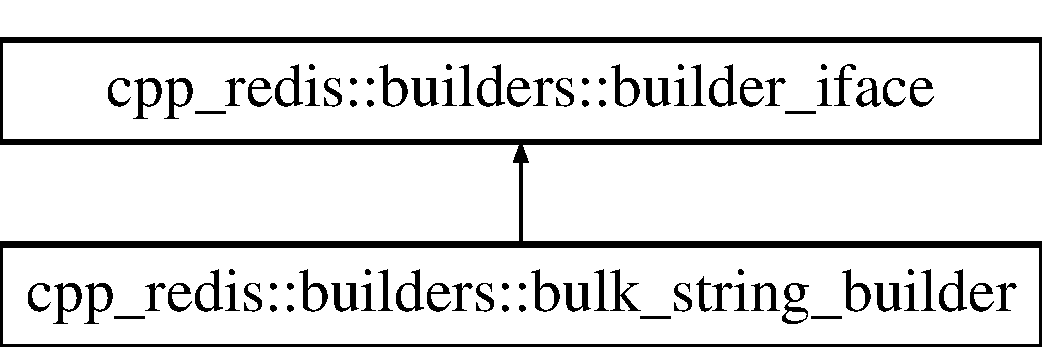
\includegraphics[height=2.000000cm]{classcpp__redis_1_1builders_1_1bulk__string__builder}
\end{center}
\end{figure}
\subsection*{Public Member Functions}
\begin{DoxyCompactItemize}
\item 
\hyperlink{classcpp__redis_1_1builders_1_1bulk__string__builder_a1c0bee3cd6fbafc782cfe93c0b650451}{bulk\+\_\+string\+\_\+builder} (void)
\begin{DoxyCompactList}\small\item\em ctor \end{DoxyCompactList}\item 
\hyperlink{classcpp__redis_1_1builders_1_1bulk__string__builder_a88c7142bab456f70da9f9a6252e2affb}{$\sim$bulk\+\_\+string\+\_\+builder} (void)=default
\begin{DoxyCompactList}\small\item\em dtor \end{DoxyCompactList}\item 
\hyperlink{classcpp__redis_1_1builders_1_1bulk__string__builder_ac3bd10f8972fa1856b6e7b7262ecd98f}{bulk\+\_\+string\+\_\+builder} (const \hyperlink{classcpp__redis_1_1builders_1_1bulk__string__builder}{bulk\+\_\+string\+\_\+builder} \&)=delete
\begin{DoxyCompactList}\small\item\em copy ctor \end{DoxyCompactList}\item 
\hyperlink{classcpp__redis_1_1builders_1_1bulk__string__builder}{bulk\+\_\+string\+\_\+builder} \& \hyperlink{classcpp__redis_1_1builders_1_1bulk__string__builder_a972355e0910faa9e3daf4f5c67c3e581}{operator=} (const \hyperlink{classcpp__redis_1_1builders_1_1bulk__string__builder}{bulk\+\_\+string\+\_\+builder} \&)=delete
\begin{DoxyCompactList}\small\item\em assignment operator \end{DoxyCompactList}\item 
\hyperlink{classcpp__redis_1_1builders_1_1builder__iface}{builder\+\_\+iface} \& \hyperlink{classcpp__redis_1_1builders_1_1bulk__string__builder_a43000357f87212f657aafe279a92b541}{operator$<$$<$} (std\+::string \&data)
\item 
bool \hyperlink{classcpp__redis_1_1builders_1_1bulk__string__builder_a4d80d8dfe305e35aca8b4ec84c56fbea}{reply\+\_\+ready} (void) const
\item 
\hyperlink{classcpp__redis_1_1reply}{reply} \hyperlink{classcpp__redis_1_1builders_1_1bulk__string__builder_a56d6d3089107a1bccd63f6a5267c16cb}{get\+\_\+reply} (void) const
\item 
const std\+::string \& \hyperlink{classcpp__redis_1_1builders_1_1bulk__string__builder_a6b3e70acab5c115609db774becbcc571}{get\+\_\+bulk\+\_\+string} (void) const
\item 
bool \hyperlink{classcpp__redis_1_1builders_1_1bulk__string__builder_a2a6ab893dbe5ad2433df18ce62ca6211}{is\+\_\+null} (void) const
\end{DoxyCompactItemize}
\subsection*{Private Member Functions}
\begin{DoxyCompactItemize}
\item 
void \hyperlink{classcpp__redis_1_1builders_1_1bulk__string__builder_a9f3622a786d17cded1bcdb99c5c3ec72}{build\+\_\+reply} (void)
\item 
bool \hyperlink{classcpp__redis_1_1builders_1_1bulk__string__builder_a5bfc13e5c3a03b73e0c0700143075797}{fetch\+\_\+size} (std\+::string \&str)
\item 
void \hyperlink{classcpp__redis_1_1builders_1_1bulk__string__builder_a0ab6e537f621fd8df0d70663920eddc7}{fetch\+\_\+str} (std\+::string \&str)
\end{DoxyCompactItemize}
\subsection*{Private Attributes}
\begin{DoxyCompactItemize}
\item 
\hyperlink{classcpp__redis_1_1builders_1_1integer__builder}{integer\+\_\+builder} \hyperlink{classcpp__redis_1_1builders_1_1bulk__string__builder_a915d9ed7510d3da74acfba316bb6552a}{m\+\_\+int\+\_\+builder}
\item 
int \hyperlink{classcpp__redis_1_1builders_1_1bulk__string__builder_afac58a56edceb0ed8b5581fc53907f58}{m\+\_\+str\+\_\+size}
\item 
std\+::string \hyperlink{classcpp__redis_1_1builders_1_1bulk__string__builder_a98a8ab86c8a6d9e6918389ca894853d3}{m\+\_\+str}
\item 
bool \hyperlink{classcpp__redis_1_1builders_1_1bulk__string__builder_af55ddd50b4d654eb41a153c77ebca8c0}{m\+\_\+is\+\_\+null}
\item 
bool \hyperlink{classcpp__redis_1_1builders_1_1bulk__string__builder_a98dfcef106c6e96e920da82773fcfb85}{m\+\_\+reply\+\_\+ready}
\item 
\hyperlink{classcpp__redis_1_1reply}{reply} \hyperlink{classcpp__redis_1_1builders_1_1bulk__string__builder_af83fb520f2a964124a95e6ba1d87c651}{m\+\_\+reply}
\end{DoxyCompactItemize}


\subsection{Detailed Description}
builder to build redis bulk string replies 

\subsection{Constructor \& Destructor Documentation}
\mbox{\Hypertarget{classcpp__redis_1_1builders_1_1bulk__string__builder_a1c0bee3cd6fbafc782cfe93c0b650451}\label{classcpp__redis_1_1builders_1_1bulk__string__builder_a1c0bee3cd6fbafc782cfe93c0b650451}} 
\index{cpp\+\_\+redis\+::builders\+::bulk\+\_\+string\+\_\+builder@{cpp\+\_\+redis\+::builders\+::bulk\+\_\+string\+\_\+builder}!bulk\+\_\+string\+\_\+builder@{bulk\+\_\+string\+\_\+builder}}
\index{bulk\+\_\+string\+\_\+builder@{bulk\+\_\+string\+\_\+builder}!cpp\+\_\+redis\+::builders\+::bulk\+\_\+string\+\_\+builder@{cpp\+\_\+redis\+::builders\+::bulk\+\_\+string\+\_\+builder}}
\subsubsection{\texorpdfstring{bulk\+\_\+string\+\_\+builder()}{bulk\_string\_builder()}\hspace{0.1cm}{\footnotesize\ttfamily [1/2]}}
{\footnotesize\ttfamily cpp\+\_\+redis\+::builders\+::bulk\+\_\+string\+\_\+builder\+::bulk\+\_\+string\+\_\+builder (\begin{DoxyParamCaption}\item[{void}]{ }\end{DoxyParamCaption})}



ctor 

\mbox{\Hypertarget{classcpp__redis_1_1builders_1_1bulk__string__builder_a88c7142bab456f70da9f9a6252e2affb}\label{classcpp__redis_1_1builders_1_1bulk__string__builder_a88c7142bab456f70da9f9a6252e2affb}} 
\index{cpp\+\_\+redis\+::builders\+::bulk\+\_\+string\+\_\+builder@{cpp\+\_\+redis\+::builders\+::bulk\+\_\+string\+\_\+builder}!````~bulk\+\_\+string\+\_\+builder@{$\sim$bulk\+\_\+string\+\_\+builder}}
\index{````~bulk\+\_\+string\+\_\+builder@{$\sim$bulk\+\_\+string\+\_\+builder}!cpp\+\_\+redis\+::builders\+::bulk\+\_\+string\+\_\+builder@{cpp\+\_\+redis\+::builders\+::bulk\+\_\+string\+\_\+builder}}
\subsubsection{\texorpdfstring{$\sim$bulk\+\_\+string\+\_\+builder()}{~bulk\_string\_builder()}}
{\footnotesize\ttfamily cpp\+\_\+redis\+::builders\+::bulk\+\_\+string\+\_\+builder\+::$\sim$bulk\+\_\+string\+\_\+builder (\begin{DoxyParamCaption}\item[{void}]{ }\end{DoxyParamCaption})\hspace{0.3cm}{\ttfamily [default]}}



dtor 

\mbox{\Hypertarget{classcpp__redis_1_1builders_1_1bulk__string__builder_ac3bd10f8972fa1856b6e7b7262ecd98f}\label{classcpp__redis_1_1builders_1_1bulk__string__builder_ac3bd10f8972fa1856b6e7b7262ecd98f}} 
\index{cpp\+\_\+redis\+::builders\+::bulk\+\_\+string\+\_\+builder@{cpp\+\_\+redis\+::builders\+::bulk\+\_\+string\+\_\+builder}!bulk\+\_\+string\+\_\+builder@{bulk\+\_\+string\+\_\+builder}}
\index{bulk\+\_\+string\+\_\+builder@{bulk\+\_\+string\+\_\+builder}!cpp\+\_\+redis\+::builders\+::bulk\+\_\+string\+\_\+builder@{cpp\+\_\+redis\+::builders\+::bulk\+\_\+string\+\_\+builder}}
\subsubsection{\texorpdfstring{bulk\+\_\+string\+\_\+builder()}{bulk\_string\_builder()}\hspace{0.1cm}{\footnotesize\ttfamily [2/2]}}
{\footnotesize\ttfamily cpp\+\_\+redis\+::builders\+::bulk\+\_\+string\+\_\+builder\+::bulk\+\_\+string\+\_\+builder (\begin{DoxyParamCaption}\item[{const \hyperlink{classcpp__redis_1_1builders_1_1bulk__string__builder}{bulk\+\_\+string\+\_\+builder} \&}]{ }\end{DoxyParamCaption})\hspace{0.3cm}{\ttfamily [delete]}}



copy ctor 



\subsection{Member Function Documentation}
\mbox{\Hypertarget{classcpp__redis_1_1builders_1_1bulk__string__builder_a9f3622a786d17cded1bcdb99c5c3ec72}\label{classcpp__redis_1_1builders_1_1bulk__string__builder_a9f3622a786d17cded1bcdb99c5c3ec72}} 
\index{cpp\+\_\+redis\+::builders\+::bulk\+\_\+string\+\_\+builder@{cpp\+\_\+redis\+::builders\+::bulk\+\_\+string\+\_\+builder}!build\+\_\+reply@{build\+\_\+reply}}
\index{build\+\_\+reply@{build\+\_\+reply}!cpp\+\_\+redis\+::builders\+::bulk\+\_\+string\+\_\+builder@{cpp\+\_\+redis\+::builders\+::bulk\+\_\+string\+\_\+builder}}
\subsubsection{\texorpdfstring{build\+\_\+reply()}{build\_reply()}}
{\footnotesize\ttfamily void cpp\+\_\+redis\+::builders\+::bulk\+\_\+string\+\_\+builder\+::build\+\_\+reply (\begin{DoxyParamCaption}\item[{void}]{ }\end{DoxyParamCaption})\hspace{0.3cm}{\ttfamily [private]}}

\mbox{\Hypertarget{classcpp__redis_1_1builders_1_1bulk__string__builder_a5bfc13e5c3a03b73e0c0700143075797}\label{classcpp__redis_1_1builders_1_1bulk__string__builder_a5bfc13e5c3a03b73e0c0700143075797}} 
\index{cpp\+\_\+redis\+::builders\+::bulk\+\_\+string\+\_\+builder@{cpp\+\_\+redis\+::builders\+::bulk\+\_\+string\+\_\+builder}!fetch\+\_\+size@{fetch\+\_\+size}}
\index{fetch\+\_\+size@{fetch\+\_\+size}!cpp\+\_\+redis\+::builders\+::bulk\+\_\+string\+\_\+builder@{cpp\+\_\+redis\+::builders\+::bulk\+\_\+string\+\_\+builder}}
\subsubsection{\texorpdfstring{fetch\+\_\+size()}{fetch\_size()}}
{\footnotesize\ttfamily bool cpp\+\_\+redis\+::builders\+::bulk\+\_\+string\+\_\+builder\+::fetch\+\_\+size (\begin{DoxyParamCaption}\item[{std\+::string \&}]{str }\end{DoxyParamCaption})\hspace{0.3cm}{\ttfamily [private]}}

\mbox{\Hypertarget{classcpp__redis_1_1builders_1_1bulk__string__builder_a0ab6e537f621fd8df0d70663920eddc7}\label{classcpp__redis_1_1builders_1_1bulk__string__builder_a0ab6e537f621fd8df0d70663920eddc7}} 
\index{cpp\+\_\+redis\+::builders\+::bulk\+\_\+string\+\_\+builder@{cpp\+\_\+redis\+::builders\+::bulk\+\_\+string\+\_\+builder}!fetch\+\_\+str@{fetch\+\_\+str}}
\index{fetch\+\_\+str@{fetch\+\_\+str}!cpp\+\_\+redis\+::builders\+::bulk\+\_\+string\+\_\+builder@{cpp\+\_\+redis\+::builders\+::bulk\+\_\+string\+\_\+builder}}
\subsubsection{\texorpdfstring{fetch\+\_\+str()}{fetch\_str()}}
{\footnotesize\ttfamily void cpp\+\_\+redis\+::builders\+::bulk\+\_\+string\+\_\+builder\+::fetch\+\_\+str (\begin{DoxyParamCaption}\item[{std\+::string \&}]{str }\end{DoxyParamCaption})\hspace{0.3cm}{\ttfamily [private]}}

\mbox{\Hypertarget{classcpp__redis_1_1builders_1_1bulk__string__builder_a6b3e70acab5c115609db774becbcc571}\label{classcpp__redis_1_1builders_1_1bulk__string__builder_a6b3e70acab5c115609db774becbcc571}} 
\index{cpp\+\_\+redis\+::builders\+::bulk\+\_\+string\+\_\+builder@{cpp\+\_\+redis\+::builders\+::bulk\+\_\+string\+\_\+builder}!get\+\_\+bulk\+\_\+string@{get\+\_\+bulk\+\_\+string}}
\index{get\+\_\+bulk\+\_\+string@{get\+\_\+bulk\+\_\+string}!cpp\+\_\+redis\+::builders\+::bulk\+\_\+string\+\_\+builder@{cpp\+\_\+redis\+::builders\+::bulk\+\_\+string\+\_\+builder}}
\subsubsection{\texorpdfstring{get\+\_\+bulk\+\_\+string()}{get\_bulk\_string()}}
{\footnotesize\ttfamily const std\+::string\& cpp\+\_\+redis\+::builders\+::bulk\+\_\+string\+\_\+builder\+::get\+\_\+bulk\+\_\+string (\begin{DoxyParamCaption}\item[{void}]{ }\end{DoxyParamCaption}) const}

\begin{DoxyReturn}{Returns}
the parsed bulk string 
\end{DoxyReturn}
\mbox{\Hypertarget{classcpp__redis_1_1builders_1_1bulk__string__builder_a56d6d3089107a1bccd63f6a5267c16cb}\label{classcpp__redis_1_1builders_1_1bulk__string__builder_a56d6d3089107a1bccd63f6a5267c16cb}} 
\index{cpp\+\_\+redis\+::builders\+::bulk\+\_\+string\+\_\+builder@{cpp\+\_\+redis\+::builders\+::bulk\+\_\+string\+\_\+builder}!get\+\_\+reply@{get\+\_\+reply}}
\index{get\+\_\+reply@{get\+\_\+reply}!cpp\+\_\+redis\+::builders\+::bulk\+\_\+string\+\_\+builder@{cpp\+\_\+redis\+::builders\+::bulk\+\_\+string\+\_\+builder}}
\subsubsection{\texorpdfstring{get\+\_\+reply()}{get\_reply()}}
{\footnotesize\ttfamily \hyperlink{classcpp__redis_1_1reply}{reply} cpp\+\_\+redis\+::builders\+::bulk\+\_\+string\+\_\+builder\+::get\+\_\+reply (\begin{DoxyParamCaption}\item[{void}]{ }\end{DoxyParamCaption}) const\hspace{0.3cm}{\ttfamily [virtual]}}

\begin{DoxyReturn}{Returns}
reply object 
\end{DoxyReturn}


Implements \hyperlink{classcpp__redis_1_1builders_1_1builder__iface_afd2ff2c2371c2a486116543b638b9413}{cpp\+\_\+redis\+::builders\+::builder\+\_\+iface}.

\mbox{\Hypertarget{classcpp__redis_1_1builders_1_1bulk__string__builder_a2a6ab893dbe5ad2433df18ce62ca6211}\label{classcpp__redis_1_1builders_1_1bulk__string__builder_a2a6ab893dbe5ad2433df18ce62ca6211}} 
\index{cpp\+\_\+redis\+::builders\+::bulk\+\_\+string\+\_\+builder@{cpp\+\_\+redis\+::builders\+::bulk\+\_\+string\+\_\+builder}!is\+\_\+null@{is\+\_\+null}}
\index{is\+\_\+null@{is\+\_\+null}!cpp\+\_\+redis\+::builders\+::bulk\+\_\+string\+\_\+builder@{cpp\+\_\+redis\+::builders\+::bulk\+\_\+string\+\_\+builder}}
\subsubsection{\texorpdfstring{is\+\_\+null()}{is\_null()}}
{\footnotesize\ttfamily bool cpp\+\_\+redis\+::builders\+::bulk\+\_\+string\+\_\+builder\+::is\+\_\+null (\begin{DoxyParamCaption}\item[{void}]{ }\end{DoxyParamCaption}) const}

\begin{DoxyReturn}{Returns}
whether the bulk string is null 
\end{DoxyReturn}
\mbox{\Hypertarget{classcpp__redis_1_1builders_1_1bulk__string__builder_a43000357f87212f657aafe279a92b541}\label{classcpp__redis_1_1builders_1_1bulk__string__builder_a43000357f87212f657aafe279a92b541}} 
\index{cpp\+\_\+redis\+::builders\+::bulk\+\_\+string\+\_\+builder@{cpp\+\_\+redis\+::builders\+::bulk\+\_\+string\+\_\+builder}!operator$<$$<$@{operator$<$$<$}}
\index{operator$<$$<$@{operator$<$$<$}!cpp\+\_\+redis\+::builders\+::bulk\+\_\+string\+\_\+builder@{cpp\+\_\+redis\+::builders\+::bulk\+\_\+string\+\_\+builder}}
\subsubsection{\texorpdfstring{operator$<$$<$()}{operator<<()}}
{\footnotesize\ttfamily \hyperlink{classcpp__redis_1_1builders_1_1builder__iface}{builder\+\_\+iface}\& cpp\+\_\+redis\+::builders\+::bulk\+\_\+string\+\_\+builder\+::operator$<$$<$ (\begin{DoxyParamCaption}\item[{std\+::string \&}]{data }\end{DoxyParamCaption})\hspace{0.3cm}{\ttfamily [virtual]}}

take data as parameter which is consumed to build the reply every bytes used to build the reply must be removed from the buffer passed as parameter


\begin{DoxyParams}{Parameters}
{\em data} & data to be consumed \\
\hline
\end{DoxyParams}
\begin{DoxyReturn}{Returns}
current instance 
\end{DoxyReturn}


Implements \hyperlink{classcpp__redis_1_1builders_1_1builder__iface_a9892bbc9c887c31c2742dad4476e2fa6}{cpp\+\_\+redis\+::builders\+::builder\+\_\+iface}.

\mbox{\Hypertarget{classcpp__redis_1_1builders_1_1bulk__string__builder_a972355e0910faa9e3daf4f5c67c3e581}\label{classcpp__redis_1_1builders_1_1bulk__string__builder_a972355e0910faa9e3daf4f5c67c3e581}} 
\index{cpp\+\_\+redis\+::builders\+::bulk\+\_\+string\+\_\+builder@{cpp\+\_\+redis\+::builders\+::bulk\+\_\+string\+\_\+builder}!operator=@{operator=}}
\index{operator=@{operator=}!cpp\+\_\+redis\+::builders\+::bulk\+\_\+string\+\_\+builder@{cpp\+\_\+redis\+::builders\+::bulk\+\_\+string\+\_\+builder}}
\subsubsection{\texorpdfstring{operator=()}{operator=()}}
{\footnotesize\ttfamily \hyperlink{classcpp__redis_1_1builders_1_1bulk__string__builder}{bulk\+\_\+string\+\_\+builder}\& cpp\+\_\+redis\+::builders\+::bulk\+\_\+string\+\_\+builder\+::operator= (\begin{DoxyParamCaption}\item[{const \hyperlink{classcpp__redis_1_1builders_1_1bulk__string__builder}{bulk\+\_\+string\+\_\+builder} \&}]{ }\end{DoxyParamCaption})\hspace{0.3cm}{\ttfamily [delete]}}



assignment operator 

\mbox{\Hypertarget{classcpp__redis_1_1builders_1_1bulk__string__builder_a4d80d8dfe305e35aca8b4ec84c56fbea}\label{classcpp__redis_1_1builders_1_1bulk__string__builder_a4d80d8dfe305e35aca8b4ec84c56fbea}} 
\index{cpp\+\_\+redis\+::builders\+::bulk\+\_\+string\+\_\+builder@{cpp\+\_\+redis\+::builders\+::bulk\+\_\+string\+\_\+builder}!reply\+\_\+ready@{reply\+\_\+ready}}
\index{reply\+\_\+ready@{reply\+\_\+ready}!cpp\+\_\+redis\+::builders\+::bulk\+\_\+string\+\_\+builder@{cpp\+\_\+redis\+::builders\+::bulk\+\_\+string\+\_\+builder}}
\subsubsection{\texorpdfstring{reply\+\_\+ready()}{reply\_ready()}}
{\footnotesize\ttfamily bool cpp\+\_\+redis\+::builders\+::bulk\+\_\+string\+\_\+builder\+::reply\+\_\+ready (\begin{DoxyParamCaption}\item[{void}]{ }\end{DoxyParamCaption}) const\hspace{0.3cm}{\ttfamily [virtual]}}

\begin{DoxyReturn}{Returns}
whether the reply could be built 
\end{DoxyReturn}


Implements \hyperlink{classcpp__redis_1_1builders_1_1builder__iface_a40db9a31d4ea1771777e74146d31e12d}{cpp\+\_\+redis\+::builders\+::builder\+\_\+iface}.



\subsection{Member Data Documentation}
\mbox{\Hypertarget{classcpp__redis_1_1builders_1_1bulk__string__builder_a915d9ed7510d3da74acfba316bb6552a}\label{classcpp__redis_1_1builders_1_1bulk__string__builder_a915d9ed7510d3da74acfba316bb6552a}} 
\index{cpp\+\_\+redis\+::builders\+::bulk\+\_\+string\+\_\+builder@{cpp\+\_\+redis\+::builders\+::bulk\+\_\+string\+\_\+builder}!m\+\_\+int\+\_\+builder@{m\+\_\+int\+\_\+builder}}
\index{m\+\_\+int\+\_\+builder@{m\+\_\+int\+\_\+builder}!cpp\+\_\+redis\+::builders\+::bulk\+\_\+string\+\_\+builder@{cpp\+\_\+redis\+::builders\+::bulk\+\_\+string\+\_\+builder}}
\subsubsection{\texorpdfstring{m\+\_\+int\+\_\+builder}{m\_int\_builder}}
{\footnotesize\ttfamily \hyperlink{classcpp__redis_1_1builders_1_1integer__builder}{integer\+\_\+builder} cpp\+\_\+redis\+::builders\+::bulk\+\_\+string\+\_\+builder\+::m\+\_\+int\+\_\+builder\hspace{0.3cm}{\ttfamily [private]}}

builder used to get bulk string size \mbox{\Hypertarget{classcpp__redis_1_1builders_1_1bulk__string__builder_af55ddd50b4d654eb41a153c77ebca8c0}\label{classcpp__redis_1_1builders_1_1bulk__string__builder_af55ddd50b4d654eb41a153c77ebca8c0}} 
\index{cpp\+\_\+redis\+::builders\+::bulk\+\_\+string\+\_\+builder@{cpp\+\_\+redis\+::builders\+::bulk\+\_\+string\+\_\+builder}!m\+\_\+is\+\_\+null@{m\+\_\+is\+\_\+null}}
\index{m\+\_\+is\+\_\+null@{m\+\_\+is\+\_\+null}!cpp\+\_\+redis\+::builders\+::bulk\+\_\+string\+\_\+builder@{cpp\+\_\+redis\+::builders\+::bulk\+\_\+string\+\_\+builder}}
\subsubsection{\texorpdfstring{m\+\_\+is\+\_\+null}{m\_is\_null}}
{\footnotesize\ttfamily bool cpp\+\_\+redis\+::builders\+::bulk\+\_\+string\+\_\+builder\+::m\+\_\+is\+\_\+null\hspace{0.3cm}{\ttfamily [private]}}

whether the bulk string is null \mbox{\Hypertarget{classcpp__redis_1_1builders_1_1bulk__string__builder_af83fb520f2a964124a95e6ba1d87c651}\label{classcpp__redis_1_1builders_1_1bulk__string__builder_af83fb520f2a964124a95e6ba1d87c651}} 
\index{cpp\+\_\+redis\+::builders\+::bulk\+\_\+string\+\_\+builder@{cpp\+\_\+redis\+::builders\+::bulk\+\_\+string\+\_\+builder}!m\+\_\+reply@{m\+\_\+reply}}
\index{m\+\_\+reply@{m\+\_\+reply}!cpp\+\_\+redis\+::builders\+::bulk\+\_\+string\+\_\+builder@{cpp\+\_\+redis\+::builders\+::bulk\+\_\+string\+\_\+builder}}
\subsubsection{\texorpdfstring{m\+\_\+reply}{m\_reply}}
{\footnotesize\ttfamily \hyperlink{classcpp__redis_1_1reply}{reply} cpp\+\_\+redis\+::builders\+::bulk\+\_\+string\+\_\+builder\+::m\+\_\+reply\hspace{0.3cm}{\ttfamily [private]}}

reply to be built \mbox{\Hypertarget{classcpp__redis_1_1builders_1_1bulk__string__builder_a98dfcef106c6e96e920da82773fcfb85}\label{classcpp__redis_1_1builders_1_1bulk__string__builder_a98dfcef106c6e96e920da82773fcfb85}} 
\index{cpp\+\_\+redis\+::builders\+::bulk\+\_\+string\+\_\+builder@{cpp\+\_\+redis\+::builders\+::bulk\+\_\+string\+\_\+builder}!m\+\_\+reply\+\_\+ready@{m\+\_\+reply\+\_\+ready}}
\index{m\+\_\+reply\+\_\+ready@{m\+\_\+reply\+\_\+ready}!cpp\+\_\+redis\+::builders\+::bulk\+\_\+string\+\_\+builder@{cpp\+\_\+redis\+::builders\+::bulk\+\_\+string\+\_\+builder}}
\subsubsection{\texorpdfstring{m\+\_\+reply\+\_\+ready}{m\_reply\_ready}}
{\footnotesize\ttfamily bool cpp\+\_\+redis\+::builders\+::bulk\+\_\+string\+\_\+builder\+::m\+\_\+reply\+\_\+ready\hspace{0.3cm}{\ttfamily [private]}}

whether the reply is ready or not \mbox{\Hypertarget{classcpp__redis_1_1builders_1_1bulk__string__builder_a98a8ab86c8a6d9e6918389ca894853d3}\label{classcpp__redis_1_1builders_1_1bulk__string__builder_a98a8ab86c8a6d9e6918389ca894853d3}} 
\index{cpp\+\_\+redis\+::builders\+::bulk\+\_\+string\+\_\+builder@{cpp\+\_\+redis\+::builders\+::bulk\+\_\+string\+\_\+builder}!m\+\_\+str@{m\+\_\+str}}
\index{m\+\_\+str@{m\+\_\+str}!cpp\+\_\+redis\+::builders\+::bulk\+\_\+string\+\_\+builder@{cpp\+\_\+redis\+::builders\+::bulk\+\_\+string\+\_\+builder}}
\subsubsection{\texorpdfstring{m\+\_\+str}{m\_str}}
{\footnotesize\ttfamily std\+::string cpp\+\_\+redis\+::builders\+::bulk\+\_\+string\+\_\+builder\+::m\+\_\+str\hspace{0.3cm}{\ttfamily [private]}}

bulk string \mbox{\Hypertarget{classcpp__redis_1_1builders_1_1bulk__string__builder_afac58a56edceb0ed8b5581fc53907f58}\label{classcpp__redis_1_1builders_1_1bulk__string__builder_afac58a56edceb0ed8b5581fc53907f58}} 
\index{cpp\+\_\+redis\+::builders\+::bulk\+\_\+string\+\_\+builder@{cpp\+\_\+redis\+::builders\+::bulk\+\_\+string\+\_\+builder}!m\+\_\+str\+\_\+size@{m\+\_\+str\+\_\+size}}
\index{m\+\_\+str\+\_\+size@{m\+\_\+str\+\_\+size}!cpp\+\_\+redis\+::builders\+::bulk\+\_\+string\+\_\+builder@{cpp\+\_\+redis\+::builders\+::bulk\+\_\+string\+\_\+builder}}
\subsubsection{\texorpdfstring{m\+\_\+str\+\_\+size}{m\_str\_size}}
{\footnotesize\ttfamily int cpp\+\_\+redis\+::builders\+::bulk\+\_\+string\+\_\+builder\+::m\+\_\+str\+\_\+size\hspace{0.3cm}{\ttfamily [private]}}

bulk string size 

The documentation for this class was generated from the following file\+:\begin{DoxyCompactItemize}
\item 
includes/cpp\+\_\+redis/builders/\hyperlink{bulk__string__builder_8hpp}{bulk\+\_\+string\+\_\+builder.\+hpp}\end{DoxyCompactItemize}

\hypertarget{classcpp__redis_1_1client}{}\section{cpp\+\_\+redis\+:\+:client Class Reference}
\label{classcpp__redis_1_1client}\index{cpp\+\_\+redis\+::client@{cpp\+\_\+redis\+::client}}
\subsection*{Public Types}
\begin{DoxyCompactItemize}
\item 
enum \hyperlink{classcpp__redis_1_1client_a388877b01b4e045cddb138e70a68e000}{client\+\_\+type} \{ {\bfseries normal}, 
{\bfseries master}, 
{\bfseries pubsub}, 
{\bfseries slave}
 \}
\item 
enum \hyperlink{classcpp__redis_1_1client_a2512bd48dd45391249a69bd720c1e4da}{connect\+\_\+state} \{ \newline
{\bfseries dropped}, 
{\bfseries start}, 
{\bfseries sleeping}, 
{\bfseries ok}, 
\newline
{\bfseries failed}, 
{\bfseries lookup\+\_\+failed}, 
{\bfseries stopped}
 \}
\item 
typedef std\+::function$<$ void(const std\+::string \&host, std\+::size\+\_\+t port, \hyperlink{classcpp__redis_1_1client_a2512bd48dd45391249a69bd720c1e4da}{connect\+\_\+state} status)$>$ \hyperlink{classcpp__redis_1_1client_a4bb592b64ededde5a6fcf8111ca2548f}{connect\+\_\+callback\+\_\+t}
\item 
typedef std\+::function$<$ void(\hyperlink{classcpp__redis_1_1reply}{reply} \&)$>$ \hyperlink{classcpp__redis_1_1client_a061a1140d36d2eaeda82b09a0bb3f9f2}{reply\+\_\+callback\+\_\+t}
\end{DoxyCompactItemize}
\subsection*{Public Member Functions}
\begin{DoxyCompactItemize}
\item 
\mbox{\Hypertarget{classcpp__redis_1_1client_a80354f41d084dfc3a41df581c803b792}\label{classcpp__redis_1_1client_a80354f41d084dfc3a41df581c803b792}} 
\hyperlink{classcpp__redis_1_1client_a80354f41d084dfc3a41df581c803b792}{client} (void)
\begin{DoxyCompactList}\small\item\em ctor \end{DoxyCompactList}\item 
\hyperlink{classcpp__redis_1_1client_ae879c3a6829a2da9d03f80c1ec4b8d9b}{client} (const std\+::shared\+\_\+ptr$<$ \hyperlink{classcpp__redis_1_1network_1_1tcp__client__iface}{network\+::tcp\+\_\+client\+\_\+iface} $>$ \&tcp\+\_\+client)
\item 
\mbox{\Hypertarget{classcpp__redis_1_1client_aca7030c8bd6856f10314b2862d1bae79}\label{classcpp__redis_1_1client_aca7030c8bd6856f10314b2862d1bae79}} 
\hyperlink{classcpp__redis_1_1client_aca7030c8bd6856f10314b2862d1bae79}{$\sim$client} (void)
\begin{DoxyCompactList}\small\item\em dtor \end{DoxyCompactList}\item 
\mbox{\Hypertarget{classcpp__redis_1_1client_ab938aeb2a144629fd269594e4af08168}\label{classcpp__redis_1_1client_ab938aeb2a144629fd269594e4af08168}} 
\hyperlink{classcpp__redis_1_1client_ab938aeb2a144629fd269594e4af08168}{client} (const \hyperlink{classcpp__redis_1_1client}{client} \&)=delete
\begin{DoxyCompactList}\small\item\em copy ctor \end{DoxyCompactList}\item 
\mbox{\Hypertarget{classcpp__redis_1_1client_afdab99b1752e759ab3ce9477f2cb092d}\label{classcpp__redis_1_1client_afdab99b1752e759ab3ce9477f2cb092d}} 
\hyperlink{classcpp__redis_1_1client}{client} \& \hyperlink{classcpp__redis_1_1client_afdab99b1752e759ab3ce9477f2cb092d}{operator=} (const \hyperlink{classcpp__redis_1_1client}{client} \&)=delete
\begin{DoxyCompactList}\small\item\em assignment operator \end{DoxyCompactList}\item 
void \hyperlink{classcpp__redis_1_1client_adda8b3e7b4f9c80ac052753b39178dd5}{connect} (const std\+::string \&host=\char`\"{}127.\+0.\+0.\+1\char`\"{}, std\+::size\+\_\+t port=6379, const \hyperlink{classcpp__redis_1_1client_a4bb592b64ededde5a6fcf8111ca2548f}{connect\+\_\+callback\+\_\+t} \&connect\+\_\+callback=nullptr, std\+::uint32\+\_\+t timeout\+\_\+msecs=0, std\+::int32\+\_\+t max\+\_\+reconnects=0, std\+::uint32\+\_\+t reconnect\+\_\+interval\+\_\+msecs=0)
\item 
void \hyperlink{classcpp__redis_1_1client_a15bcb0885129480543482a7da52af892}{connect} (const std\+::string \&name, const \hyperlink{classcpp__redis_1_1client_a4bb592b64ededde5a6fcf8111ca2548f}{connect\+\_\+callback\+\_\+t} \&connect\+\_\+callback=nullptr, std\+::uint32\+\_\+t timeout\+\_\+msecs=0, std\+::int32\+\_\+t max\+\_\+reconnects=0, std\+::uint32\+\_\+t reconnect\+\_\+interval\+\_\+msecs=0)
\item 
bool \hyperlink{classcpp__redis_1_1client_ad3608dec2c2bfabf2c621ce14f4db37a}{is\+\_\+connected} (void) const
\item 
void \hyperlink{classcpp__redis_1_1client_a292252b61bcfdf9ad3854b54b7fe2740}{disconnect} (bool wait\+\_\+for\+\_\+removal=false)
\item 
bool \hyperlink{classcpp__redis_1_1client_af03ca1aec6416ab35e6aea93c74d89d1}{is\+\_\+reconnecting} (void) const
\item 
void \hyperlink{classcpp__redis_1_1client_adb605a877f65b8f54725576b45aeeca6}{cancel\+\_\+reconnect} (void)
\item 
\hyperlink{classcpp__redis_1_1client}{client} \& \hyperlink{classcpp__redis_1_1client_a490ef812b666e6d845fcacc808b87bc1}{send} (const std\+::vector$<$ std\+::string $>$ \&redis\+\_\+cmd, const \hyperlink{classcpp__redis_1_1client_a061a1140d36d2eaeda82b09a0bb3f9f2}{reply\+\_\+callback\+\_\+t} \&callback)
\item 
std\+::future$<$ \hyperlink{classcpp__redis_1_1reply}{reply} $>$ \hyperlink{classcpp__redis_1_1client_ad6216d6587d50694c16d68e8e182b0be}{send} (const std\+::vector$<$ std\+::string $>$ \&redis\+\_\+cmd)
\item 
\hyperlink{classcpp__redis_1_1client}{client} \& \hyperlink{classcpp__redis_1_1client_a36a48d61a4900e88fd67795ca59cbea3}{commit} (void)
\item 
\hyperlink{classcpp__redis_1_1client}{client} \& \hyperlink{classcpp__redis_1_1client_a23c8a27ee691c52713411ae91e1391fb}{sync\+\_\+commit} (void)
\item 
{\footnotesize template$<$class Rep , class Period $>$ }\\\hyperlink{classcpp__redis_1_1client}{client} \& \hyperlink{classcpp__redis_1_1client_a79a24c8367cb1229fd2c4c38d0f82533}{sync\+\_\+commit} (const std\+::chrono\+::duration$<$ Rep, Period $>$ \&timeout)
\item 
void \hyperlink{classcpp__redis_1_1client_a7050eb52856decad9ab2060a139f4b48}{add\+\_\+sentinel} (const std\+::string \&host, std\+::size\+\_\+t port)
\item 
const \hyperlink{classcpp__redis_1_1sentinel}{sentinel} \& \hyperlink{classcpp__redis_1_1client_a9f94860dad26bca4e860a56ca8aefe36}{get\+\_\+sentinel} (void) const
\item 
\hyperlink{classcpp__redis_1_1sentinel}{sentinel} \& \hyperlink{classcpp__redis_1_1client_a9457cea98f061ce6071f897ba8605813}{get\+\_\+sentinel} (void)
\item 
void \hyperlink{classcpp__redis_1_1client_a68cd15d1cc30302237e3a400e2ac43f5}{clear\+\_\+sentinels} (void)
\item 
\mbox{\Hypertarget{classcpp__redis_1_1client_ad60647638d8758103e98894457652b84}\label{classcpp__redis_1_1client_ad60647638d8758103e98894457652b84}} 
\hyperlink{classcpp__redis_1_1client}{client} \& {\bfseries append} (const std\+::string \&key, const std\+::string \&value, const \hyperlink{classcpp__redis_1_1client_a061a1140d36d2eaeda82b09a0bb3f9f2}{reply\+\_\+callback\+\_\+t} \&reply\+\_\+callback)
\item 
\mbox{\Hypertarget{classcpp__redis_1_1client_a3e50dddad0b4c9eca58d970bdc4e78da}\label{classcpp__redis_1_1client_a3e50dddad0b4c9eca58d970bdc4e78da}} 
std\+::future$<$ \hyperlink{classcpp__redis_1_1reply}{reply} $>$ {\bfseries append} (const std\+::string \&key, const std\+::string \&value)
\item 
\mbox{\Hypertarget{classcpp__redis_1_1client_a3ee834ca9c0810d2eafcf04de9dc0670}\label{classcpp__redis_1_1client_a3ee834ca9c0810d2eafcf04de9dc0670}} 
\hyperlink{classcpp__redis_1_1client}{client} \& {\bfseries auth} (const std\+::string \&password, const \hyperlink{classcpp__redis_1_1client_a061a1140d36d2eaeda82b09a0bb3f9f2}{reply\+\_\+callback\+\_\+t} \&reply\+\_\+callback)
\item 
\mbox{\Hypertarget{classcpp__redis_1_1client_a899b98d4d6da0ffdf8780933fe088fd1}\label{classcpp__redis_1_1client_a899b98d4d6da0ffdf8780933fe088fd1}} 
std\+::future$<$ \hyperlink{classcpp__redis_1_1reply}{reply} $>$ {\bfseries auth} (const std\+::string \&password)
\item 
\mbox{\Hypertarget{classcpp__redis_1_1client_a9873619c2c1ff820fde17e27ade096c8}\label{classcpp__redis_1_1client_a9873619c2c1ff820fde17e27ade096c8}} 
\hyperlink{classcpp__redis_1_1client}{client} \& {\bfseries bgrewriteaof} (const \hyperlink{classcpp__redis_1_1client_a061a1140d36d2eaeda82b09a0bb3f9f2}{reply\+\_\+callback\+\_\+t} \&reply\+\_\+callback)
\item 
\mbox{\Hypertarget{classcpp__redis_1_1client_a82959607f4cbe9dac195d27621a9cc64}\label{classcpp__redis_1_1client_a82959607f4cbe9dac195d27621a9cc64}} 
std\+::future$<$ \hyperlink{classcpp__redis_1_1reply}{reply} $>$ {\bfseries bgrewriteaof} ()
\item 
\mbox{\Hypertarget{classcpp__redis_1_1client_a102a4f3572072a5bc26681082ad16a2b}\label{classcpp__redis_1_1client_a102a4f3572072a5bc26681082ad16a2b}} 
\hyperlink{classcpp__redis_1_1client}{client} \& {\bfseries bgsave} (const \hyperlink{classcpp__redis_1_1client_a061a1140d36d2eaeda82b09a0bb3f9f2}{reply\+\_\+callback\+\_\+t} \&reply\+\_\+callback)
\item 
\mbox{\Hypertarget{classcpp__redis_1_1client_a632ef40c52f46eb4948768006adfead5}\label{classcpp__redis_1_1client_a632ef40c52f46eb4948768006adfead5}} 
std\+::future$<$ \hyperlink{classcpp__redis_1_1reply}{reply} $>$ {\bfseries bgsave} ()
\item 
\mbox{\Hypertarget{classcpp__redis_1_1client_aa6c9c15d8676a1cee3d8409ab898a049}\label{classcpp__redis_1_1client_aa6c9c15d8676a1cee3d8409ab898a049}} 
\hyperlink{classcpp__redis_1_1client}{client} \& {\bfseries bitcount} (const std\+::string \&key, const \hyperlink{classcpp__redis_1_1client_a061a1140d36d2eaeda82b09a0bb3f9f2}{reply\+\_\+callback\+\_\+t} \&reply\+\_\+callback)
\item 
\mbox{\Hypertarget{classcpp__redis_1_1client_ac667b96661726874bc237c84de1ddd89}\label{classcpp__redis_1_1client_ac667b96661726874bc237c84de1ddd89}} 
std\+::future$<$ \hyperlink{classcpp__redis_1_1reply}{reply} $>$ {\bfseries bitcount} (const std\+::string \&key)
\item 
\mbox{\Hypertarget{classcpp__redis_1_1client_ac631a06c8b69a2f1b4de3aabc19d68e2}\label{classcpp__redis_1_1client_ac631a06c8b69a2f1b4de3aabc19d68e2}} 
\hyperlink{classcpp__redis_1_1client}{client} \& {\bfseries bitcount} (const std\+::string \&key, int start, int end, const \hyperlink{classcpp__redis_1_1client_a061a1140d36d2eaeda82b09a0bb3f9f2}{reply\+\_\+callback\+\_\+t} \&reply\+\_\+callback)
\item 
\mbox{\Hypertarget{classcpp__redis_1_1client_af2d2dc1c19d735e84d8e2725fb98dbda}\label{classcpp__redis_1_1client_af2d2dc1c19d735e84d8e2725fb98dbda}} 
std\+::future$<$ \hyperlink{classcpp__redis_1_1reply}{reply} $>$ {\bfseries bitcount} (const std\+::string \&key, int start, int end)
\item 
\mbox{\Hypertarget{classcpp__redis_1_1client_a9289b0f474073f59509b565d93c69506}\label{classcpp__redis_1_1client_a9289b0f474073f59509b565d93c69506}} 
\hyperlink{classcpp__redis_1_1client}{client} \& {\bfseries bitop} (const std\+::string \&operation, const std\+::string \&destkey, const std\+::vector$<$ std\+::string $>$ \&keys, const \hyperlink{classcpp__redis_1_1client_a061a1140d36d2eaeda82b09a0bb3f9f2}{reply\+\_\+callback\+\_\+t} \&reply\+\_\+callback)
\item 
\mbox{\Hypertarget{classcpp__redis_1_1client_adbb955ee435dea43898ef811b31421b3}\label{classcpp__redis_1_1client_adbb955ee435dea43898ef811b31421b3}} 
std\+::future$<$ \hyperlink{classcpp__redis_1_1reply}{reply} $>$ {\bfseries bitop} (const std\+::string \&operation, const std\+::string \&destkey, const std\+::vector$<$ std\+::string $>$ \&keys)
\item 
\mbox{\Hypertarget{classcpp__redis_1_1client_adf2ef5d020a8efbf6f6eb91cde63f262}\label{classcpp__redis_1_1client_adf2ef5d020a8efbf6f6eb91cde63f262}} 
\hyperlink{classcpp__redis_1_1client}{client} \& {\bfseries bitpos} (const std\+::string \&key, int bit, const \hyperlink{classcpp__redis_1_1client_a061a1140d36d2eaeda82b09a0bb3f9f2}{reply\+\_\+callback\+\_\+t} \&reply\+\_\+callback)
\item 
\mbox{\Hypertarget{classcpp__redis_1_1client_a5be47a4b3f9a36c4fab420468d50256a}\label{classcpp__redis_1_1client_a5be47a4b3f9a36c4fab420468d50256a}} 
std\+::future$<$ \hyperlink{classcpp__redis_1_1reply}{reply} $>$ {\bfseries bitpos} (const std\+::string \&key, int bit)
\item 
\mbox{\Hypertarget{classcpp__redis_1_1client_a8f6b7958a3094c975c3ca053b263c523}\label{classcpp__redis_1_1client_a8f6b7958a3094c975c3ca053b263c523}} 
\hyperlink{classcpp__redis_1_1client}{client} \& {\bfseries bitpos} (const std\+::string \&key, int bit, int start, const \hyperlink{classcpp__redis_1_1client_a061a1140d36d2eaeda82b09a0bb3f9f2}{reply\+\_\+callback\+\_\+t} \&reply\+\_\+callback)
\item 
\mbox{\Hypertarget{classcpp__redis_1_1client_aa0ae004e45eb37ffed4d8c9f5ea35b4c}\label{classcpp__redis_1_1client_aa0ae004e45eb37ffed4d8c9f5ea35b4c}} 
std\+::future$<$ \hyperlink{classcpp__redis_1_1reply}{reply} $>$ {\bfseries bitpos} (const std\+::string \&key, int bit, int start)
\item 
\mbox{\Hypertarget{classcpp__redis_1_1client_a3655449a666a9111d3dce7e61932ab1b}\label{classcpp__redis_1_1client_a3655449a666a9111d3dce7e61932ab1b}} 
\hyperlink{classcpp__redis_1_1client}{client} \& {\bfseries bitpos} (const std\+::string \&key, int bit, int start, int end, const \hyperlink{classcpp__redis_1_1client_a061a1140d36d2eaeda82b09a0bb3f9f2}{reply\+\_\+callback\+\_\+t} \&reply\+\_\+callback)
\item 
\mbox{\Hypertarget{classcpp__redis_1_1client_a43b5121105276ccae731bb6093c80e02}\label{classcpp__redis_1_1client_a43b5121105276ccae731bb6093c80e02}} 
std\+::future$<$ \hyperlink{classcpp__redis_1_1reply}{reply} $>$ {\bfseries bitpos} (const std\+::string \&key, int bit, int start, int end)
\item 
\mbox{\Hypertarget{classcpp__redis_1_1client_a432c2677b13dc8e2a9d7afe7eade39e3}\label{classcpp__redis_1_1client_a432c2677b13dc8e2a9d7afe7eade39e3}} 
\hyperlink{classcpp__redis_1_1client}{client} \& {\bfseries blpop} (const std\+::vector$<$ std\+::string $>$ \&keys, int timeout, const \hyperlink{classcpp__redis_1_1client_a061a1140d36d2eaeda82b09a0bb3f9f2}{reply\+\_\+callback\+\_\+t} \&reply\+\_\+callback)
\item 
\mbox{\Hypertarget{classcpp__redis_1_1client_ac54c987bca4efb4bf6659b063f19d5ff}\label{classcpp__redis_1_1client_ac54c987bca4efb4bf6659b063f19d5ff}} 
std\+::future$<$ \hyperlink{classcpp__redis_1_1reply}{reply} $>$ {\bfseries blpop} (const std\+::vector$<$ std\+::string $>$ \&keys, int timeout)
\item 
\mbox{\Hypertarget{classcpp__redis_1_1client_adc565332168e31ebbd762f2cb12ad4d1}\label{classcpp__redis_1_1client_adc565332168e31ebbd762f2cb12ad4d1}} 
\hyperlink{classcpp__redis_1_1client}{client} \& {\bfseries brpop} (const std\+::vector$<$ std\+::string $>$ \&keys, int timeout, const \hyperlink{classcpp__redis_1_1client_a061a1140d36d2eaeda82b09a0bb3f9f2}{reply\+\_\+callback\+\_\+t} \&reply\+\_\+callback)
\item 
\mbox{\Hypertarget{classcpp__redis_1_1client_aa123b931c6d00027d08f0fcbde2f026e}\label{classcpp__redis_1_1client_aa123b931c6d00027d08f0fcbde2f026e}} 
std\+::future$<$ \hyperlink{classcpp__redis_1_1reply}{reply} $>$ {\bfseries brpop} (const std\+::vector$<$ std\+::string $>$ \&keys, int timeout)
\item 
\mbox{\Hypertarget{classcpp__redis_1_1client_afa7fb97bb0b30c2c78a605f48b6144e2}\label{classcpp__redis_1_1client_afa7fb97bb0b30c2c78a605f48b6144e2}} 
\hyperlink{classcpp__redis_1_1client}{client} \& {\bfseries brpoplpush} (const std\+::string \&src, const std\+::string \&dst, int timeout, const \hyperlink{classcpp__redis_1_1client_a061a1140d36d2eaeda82b09a0bb3f9f2}{reply\+\_\+callback\+\_\+t} \&reply\+\_\+callback)
\item 
\mbox{\Hypertarget{classcpp__redis_1_1client_aa30b9303ee0d59b07dd656db2426547e}\label{classcpp__redis_1_1client_aa30b9303ee0d59b07dd656db2426547e}} 
std\+::future$<$ \hyperlink{classcpp__redis_1_1reply}{reply} $>$ {\bfseries brpoplpush} (const std\+::string \&src, const std\+::string \&dst, int timeout)
\item 
{\footnotesize template$<$typename T , typename... Ts$>$ }\\\hyperlink{classcpp__redis_1_1client}{client} \& \hyperlink{classcpp__redis_1_1client_ae4090830d1710276c33ff5a74eba2e4b}{client\+\_\+kill} (const std\+::string \&host, int port, const T \&arg, const Ts \&... args)
\item 
\mbox{\Hypertarget{classcpp__redis_1_1client_a3163e1f29d65a5e7b0d4165be154fb96}\label{classcpp__redis_1_1client_a3163e1f29d65a5e7b0d4165be154fb96}} 
\hyperlink{classcpp__redis_1_1client}{client} \& {\bfseries client\+\_\+kill} (const std\+::string \&host, int port)
\item 
\mbox{\Hypertarget{classcpp__redis_1_1client_a38df8e614a5ac9533a1993b7dec7be6b}\label{classcpp__redis_1_1client_a38df8e614a5ac9533a1993b7dec7be6b}} 
{\footnotesize template$<$typename... Ts$>$ }\\\hyperlink{classcpp__redis_1_1client}{client} \& {\bfseries client\+\_\+kill} (const char $\ast$host, int port, const Ts \&... args)
\item 
\mbox{\Hypertarget{classcpp__redis_1_1client_a1e2dd6cdcdb4307ceda0f866fe0a154f}\label{classcpp__redis_1_1client_a1e2dd6cdcdb4307ceda0f866fe0a154f}} 
{\footnotesize template$<$typename T , typename... Ts$>$ }\\\hyperlink{classcpp__redis_1_1client}{client} \& {\bfseries client\+\_\+kill} (const T \&, const Ts \&...)
\item 
{\footnotesize template$<$typename T , typename... Ts$>$ }\\std\+::future$<$ \hyperlink{classcpp__redis_1_1reply}{reply} $>$ \hyperlink{classcpp__redis_1_1client_ae6f09b6c022c910b79fb90a47291f511}{client\+\_\+kill\+\_\+future} (const T, const Ts...)
\item 
\mbox{\Hypertarget{classcpp__redis_1_1client_a9c2e307ab54f42ce50bdd42e1c6a363b}\label{classcpp__redis_1_1client_a9c2e307ab54f42ce50bdd42e1c6a363b}} 
\hyperlink{classcpp__redis_1_1client}{client} \& {\bfseries client\+\_\+list} (const \hyperlink{classcpp__redis_1_1client_a061a1140d36d2eaeda82b09a0bb3f9f2}{reply\+\_\+callback\+\_\+t} \&reply\+\_\+callback)
\item 
\mbox{\Hypertarget{classcpp__redis_1_1client_a0480140cc584e6dd2a0a6fab9da10cc5}\label{classcpp__redis_1_1client_a0480140cc584e6dd2a0a6fab9da10cc5}} 
std\+::future$<$ \hyperlink{classcpp__redis_1_1reply}{reply} $>$ {\bfseries client\+\_\+list} ()
\item 
\mbox{\Hypertarget{classcpp__redis_1_1client_ac4e058eaa75eb04c7a8017a779d5015e}\label{classcpp__redis_1_1client_ac4e058eaa75eb04c7a8017a779d5015e}} 
\hyperlink{classcpp__redis_1_1client}{client} \& {\bfseries client\+\_\+getname} (const \hyperlink{classcpp__redis_1_1client_a061a1140d36d2eaeda82b09a0bb3f9f2}{reply\+\_\+callback\+\_\+t} \&reply\+\_\+callback)
\item 
\mbox{\Hypertarget{classcpp__redis_1_1client_a89068e68b418906e9e34cb9a95f7a179}\label{classcpp__redis_1_1client_a89068e68b418906e9e34cb9a95f7a179}} 
std\+::future$<$ \hyperlink{classcpp__redis_1_1reply}{reply} $>$ {\bfseries client\+\_\+getname} ()
\item 
\mbox{\Hypertarget{classcpp__redis_1_1client_acdf001d60d1d82d3f090b7c679e3183e}\label{classcpp__redis_1_1client_acdf001d60d1d82d3f090b7c679e3183e}} 
\hyperlink{classcpp__redis_1_1client}{client} \& {\bfseries client\+\_\+pause} (int timeout, const \hyperlink{classcpp__redis_1_1client_a061a1140d36d2eaeda82b09a0bb3f9f2}{reply\+\_\+callback\+\_\+t} \&reply\+\_\+callback)
\item 
\mbox{\Hypertarget{classcpp__redis_1_1client_a2c73a6f9b2e3f1a0afbaca9fddd29199}\label{classcpp__redis_1_1client_a2c73a6f9b2e3f1a0afbaca9fddd29199}} 
std\+::future$<$ \hyperlink{classcpp__redis_1_1reply}{reply} $>$ {\bfseries client\+\_\+pause} (int timeout)
\item 
\mbox{\Hypertarget{classcpp__redis_1_1client_a5e49e9bf9bb72659b33013fac751a712}\label{classcpp__redis_1_1client_a5e49e9bf9bb72659b33013fac751a712}} 
\hyperlink{classcpp__redis_1_1client}{client} \& {\bfseries client\+\_\+reply} (const std\+::string \&mode, const \hyperlink{classcpp__redis_1_1client_a061a1140d36d2eaeda82b09a0bb3f9f2}{reply\+\_\+callback\+\_\+t} \&reply\+\_\+callback)
\item 
\mbox{\Hypertarget{classcpp__redis_1_1client_a1b378de0c1805069b9bbecd4fca4091c}\label{classcpp__redis_1_1client_a1b378de0c1805069b9bbecd4fca4091c}} 
std\+::future$<$ \hyperlink{classcpp__redis_1_1reply}{reply} $>$ {\bfseries client\+\_\+reply} (const std\+::string \&mode)
\item 
\mbox{\Hypertarget{classcpp__redis_1_1client_a5c7f977196c1c00e3c732615c0d86ae7}\label{classcpp__redis_1_1client_a5c7f977196c1c00e3c732615c0d86ae7}} 
\hyperlink{classcpp__redis_1_1client}{client} \& {\bfseries client\+\_\+setname} (const std\+::string \&name, const \hyperlink{classcpp__redis_1_1client_a061a1140d36d2eaeda82b09a0bb3f9f2}{reply\+\_\+callback\+\_\+t} \&reply\+\_\+callback)
\item 
\mbox{\Hypertarget{classcpp__redis_1_1client_aa1ab41fda6b2536f652720b7720a0b63}\label{classcpp__redis_1_1client_aa1ab41fda6b2536f652720b7720a0b63}} 
std\+::future$<$ \hyperlink{classcpp__redis_1_1reply}{reply} $>$ {\bfseries client\+\_\+setname} (const std\+::string \&name)
\item 
\mbox{\Hypertarget{classcpp__redis_1_1client_ac156d5593e1800742188f0eee9016a84}\label{classcpp__redis_1_1client_ac156d5593e1800742188f0eee9016a84}} 
\hyperlink{classcpp__redis_1_1client}{client} \& {\bfseries cluster\+\_\+addslots} (const std\+::vector$<$ std\+::string $>$ \&p\+\_\+slots, const \hyperlink{classcpp__redis_1_1client_a061a1140d36d2eaeda82b09a0bb3f9f2}{reply\+\_\+callback\+\_\+t} \&reply\+\_\+callback)
\item 
\mbox{\Hypertarget{classcpp__redis_1_1client_a0e14578c1addf1de66745a8a95e66aeb}\label{classcpp__redis_1_1client_a0e14578c1addf1de66745a8a95e66aeb}} 
std\+::future$<$ \hyperlink{classcpp__redis_1_1reply}{reply} $>$ {\bfseries cluster\+\_\+addslots} (const std\+::vector$<$ std\+::string $>$ \&p\+\_\+slots)
\item 
\mbox{\Hypertarget{classcpp__redis_1_1client_a757c2a5c8e5b42ccd3930d89d739f602}\label{classcpp__redis_1_1client_a757c2a5c8e5b42ccd3930d89d739f602}} 
\hyperlink{classcpp__redis_1_1client}{client} \& {\bfseries cluster\+\_\+count\+\_\+failure\+\_\+reports} (const std\+::string \&node\+\_\+id, const \hyperlink{classcpp__redis_1_1client_a061a1140d36d2eaeda82b09a0bb3f9f2}{reply\+\_\+callback\+\_\+t} \&reply\+\_\+callback)
\item 
\mbox{\Hypertarget{classcpp__redis_1_1client_af1ff307eb9feb58b48b11bda78131a20}\label{classcpp__redis_1_1client_af1ff307eb9feb58b48b11bda78131a20}} 
std\+::future$<$ \hyperlink{classcpp__redis_1_1reply}{reply} $>$ {\bfseries cluster\+\_\+count\+\_\+failure\+\_\+reports} (const std\+::string \&node\+\_\+id)
\item 
\mbox{\Hypertarget{classcpp__redis_1_1client_a78017860625d016074d0495c24c3f9e8}\label{classcpp__redis_1_1client_a78017860625d016074d0495c24c3f9e8}} 
\hyperlink{classcpp__redis_1_1client}{client} \& {\bfseries cluster\+\_\+countkeysinslot} (const std\+::string \&slot, const \hyperlink{classcpp__redis_1_1client_a061a1140d36d2eaeda82b09a0bb3f9f2}{reply\+\_\+callback\+\_\+t} \&reply\+\_\+callback)
\item 
\mbox{\Hypertarget{classcpp__redis_1_1client_a8135eee3cfc95b061aee9b6f7271efce}\label{classcpp__redis_1_1client_a8135eee3cfc95b061aee9b6f7271efce}} 
std\+::future$<$ \hyperlink{classcpp__redis_1_1reply}{reply} $>$ {\bfseries cluster\+\_\+countkeysinslot} (const std\+::string \&slot)
\item 
\mbox{\Hypertarget{classcpp__redis_1_1client_a41f96bb9a627724570f1866d0983d7b2}\label{classcpp__redis_1_1client_a41f96bb9a627724570f1866d0983d7b2}} 
\hyperlink{classcpp__redis_1_1client}{client} \& {\bfseries cluster\+\_\+delslots} (const std\+::vector$<$ std\+::string $>$ \&p\+\_\+slots, const \hyperlink{classcpp__redis_1_1client_a061a1140d36d2eaeda82b09a0bb3f9f2}{reply\+\_\+callback\+\_\+t} \&reply\+\_\+callback)
\item 
\mbox{\Hypertarget{classcpp__redis_1_1client_a6cd07520f60ee78c4603211273adcf46}\label{classcpp__redis_1_1client_a6cd07520f60ee78c4603211273adcf46}} 
std\+::future$<$ \hyperlink{classcpp__redis_1_1reply}{reply} $>$ {\bfseries cluster\+\_\+delslots} (const std\+::vector$<$ std\+::string $>$ \&p\+\_\+slots)
\item 
\mbox{\Hypertarget{classcpp__redis_1_1client_a5afcee001e210150803a95c3d6412998}\label{classcpp__redis_1_1client_a5afcee001e210150803a95c3d6412998}} 
\hyperlink{classcpp__redis_1_1client}{client} \& {\bfseries cluster\+\_\+failover} (const \hyperlink{classcpp__redis_1_1client_a061a1140d36d2eaeda82b09a0bb3f9f2}{reply\+\_\+callback\+\_\+t} \&reply\+\_\+callback)
\item 
\mbox{\Hypertarget{classcpp__redis_1_1client_a76122bb138c12b90c78c4e511f45ef17}\label{classcpp__redis_1_1client_a76122bb138c12b90c78c4e511f45ef17}} 
std\+::future$<$ \hyperlink{classcpp__redis_1_1reply}{reply} $>$ {\bfseries cluster\+\_\+failover} ()
\item 
\mbox{\Hypertarget{classcpp__redis_1_1client_a9c95de64e422c09c2180dc69db386d06}\label{classcpp__redis_1_1client_a9c95de64e422c09c2180dc69db386d06}} 
\hyperlink{classcpp__redis_1_1client}{client} \& {\bfseries cluster\+\_\+failover} (const std\+::string \&mode, const \hyperlink{classcpp__redis_1_1client_a061a1140d36d2eaeda82b09a0bb3f9f2}{reply\+\_\+callback\+\_\+t} \&reply\+\_\+callback)
\item 
\mbox{\Hypertarget{classcpp__redis_1_1client_a06f9c7d27f961787b01a01be95f1fa29}\label{classcpp__redis_1_1client_a06f9c7d27f961787b01a01be95f1fa29}} 
std\+::future$<$ \hyperlink{classcpp__redis_1_1reply}{reply} $>$ {\bfseries cluster\+\_\+failover} (const std\+::string \&mode)
\item 
\mbox{\Hypertarget{classcpp__redis_1_1client_aea8a77acb9031fd03f8ab5dc2c09a17d}\label{classcpp__redis_1_1client_aea8a77acb9031fd03f8ab5dc2c09a17d}} 
\hyperlink{classcpp__redis_1_1client}{client} \& {\bfseries cluster\+\_\+forget} (const std\+::string \&node\+\_\+id, const \hyperlink{classcpp__redis_1_1client_a061a1140d36d2eaeda82b09a0bb3f9f2}{reply\+\_\+callback\+\_\+t} \&reply\+\_\+callback)
\item 
\mbox{\Hypertarget{classcpp__redis_1_1client_a58457400352dee764066bd9f737f667a}\label{classcpp__redis_1_1client_a58457400352dee764066bd9f737f667a}} 
std\+::future$<$ \hyperlink{classcpp__redis_1_1reply}{reply} $>$ {\bfseries cluster\+\_\+forget} (const std\+::string \&node\+\_\+id)
\item 
\mbox{\Hypertarget{classcpp__redis_1_1client_a716e31987800e3ca5483f72972fecfb0}\label{classcpp__redis_1_1client_a716e31987800e3ca5483f72972fecfb0}} 
\hyperlink{classcpp__redis_1_1client}{client} \& {\bfseries cluster\+\_\+getkeysinslot} (const std\+::string \&slot, int count, const \hyperlink{classcpp__redis_1_1client_a061a1140d36d2eaeda82b09a0bb3f9f2}{reply\+\_\+callback\+\_\+t} \&reply\+\_\+callback)
\item 
\mbox{\Hypertarget{classcpp__redis_1_1client_ad644ef5c24f3eb51de30a827753cc077}\label{classcpp__redis_1_1client_ad644ef5c24f3eb51de30a827753cc077}} 
std\+::future$<$ \hyperlink{classcpp__redis_1_1reply}{reply} $>$ {\bfseries cluster\+\_\+getkeysinslot} (const std\+::string \&slot, int count)
\item 
\mbox{\Hypertarget{classcpp__redis_1_1client_a831d52a9dc9115e817bae15db0fb18a6}\label{classcpp__redis_1_1client_a831d52a9dc9115e817bae15db0fb18a6}} 
\hyperlink{classcpp__redis_1_1client}{client} \& {\bfseries cluster\+\_\+info} (const \hyperlink{classcpp__redis_1_1client_a061a1140d36d2eaeda82b09a0bb3f9f2}{reply\+\_\+callback\+\_\+t} \&reply\+\_\+callback)
\item 
\mbox{\Hypertarget{classcpp__redis_1_1client_a993170e08c425a810fa757bd4c202d10}\label{classcpp__redis_1_1client_a993170e08c425a810fa757bd4c202d10}} 
std\+::future$<$ \hyperlink{classcpp__redis_1_1reply}{reply} $>$ {\bfseries cluster\+\_\+info} ()
\item 
\mbox{\Hypertarget{classcpp__redis_1_1client_ae0314fc2697674f4be4fca1cc5cbd4a1}\label{classcpp__redis_1_1client_ae0314fc2697674f4be4fca1cc5cbd4a1}} 
\hyperlink{classcpp__redis_1_1client}{client} \& {\bfseries cluster\+\_\+keyslot} (const std\+::string \&key, const \hyperlink{classcpp__redis_1_1client_a061a1140d36d2eaeda82b09a0bb3f9f2}{reply\+\_\+callback\+\_\+t} \&reply\+\_\+callback)
\item 
\mbox{\Hypertarget{classcpp__redis_1_1client_a5681ac2dfdacc19cde1a828d8b801df1}\label{classcpp__redis_1_1client_a5681ac2dfdacc19cde1a828d8b801df1}} 
std\+::future$<$ \hyperlink{classcpp__redis_1_1reply}{reply} $>$ {\bfseries cluster\+\_\+keyslot} (const std\+::string \&key)
\item 
\mbox{\Hypertarget{classcpp__redis_1_1client_aefc94be1dc7eb11673ba92bc8cbffdcf}\label{classcpp__redis_1_1client_aefc94be1dc7eb11673ba92bc8cbffdcf}} 
\hyperlink{classcpp__redis_1_1client}{client} \& {\bfseries cluster\+\_\+meet} (const std\+::string \&ip, int port, const \hyperlink{classcpp__redis_1_1client_a061a1140d36d2eaeda82b09a0bb3f9f2}{reply\+\_\+callback\+\_\+t} \&reply\+\_\+callback)
\item 
\mbox{\Hypertarget{classcpp__redis_1_1client_af142b166d5f88f76f5fd46e6e33c0523}\label{classcpp__redis_1_1client_af142b166d5f88f76f5fd46e6e33c0523}} 
std\+::future$<$ \hyperlink{classcpp__redis_1_1reply}{reply} $>$ {\bfseries cluster\+\_\+meet} (const std\+::string \&ip, int port)
\item 
\mbox{\Hypertarget{classcpp__redis_1_1client_a1e4cc880ce249fcad1b1f6ddd15f515f}\label{classcpp__redis_1_1client_a1e4cc880ce249fcad1b1f6ddd15f515f}} 
\hyperlink{classcpp__redis_1_1client}{client} \& {\bfseries cluster\+\_\+nodes} (const \hyperlink{classcpp__redis_1_1client_a061a1140d36d2eaeda82b09a0bb3f9f2}{reply\+\_\+callback\+\_\+t} \&reply\+\_\+callback)
\item 
\mbox{\Hypertarget{classcpp__redis_1_1client_a6e777dc7b54ecb4aff3e1c281f92dd81}\label{classcpp__redis_1_1client_a6e777dc7b54ecb4aff3e1c281f92dd81}} 
std\+::future$<$ \hyperlink{classcpp__redis_1_1reply}{reply} $>$ {\bfseries cluster\+\_\+nodes} ()
\item 
\mbox{\Hypertarget{classcpp__redis_1_1client_a65688223390e47c0400ba4a128000f89}\label{classcpp__redis_1_1client_a65688223390e47c0400ba4a128000f89}} 
\hyperlink{classcpp__redis_1_1client}{client} \& {\bfseries cluster\+\_\+replicate} (const std\+::string \&node\+\_\+id, const \hyperlink{classcpp__redis_1_1client_a061a1140d36d2eaeda82b09a0bb3f9f2}{reply\+\_\+callback\+\_\+t} \&reply\+\_\+callback)
\item 
\mbox{\Hypertarget{classcpp__redis_1_1client_a4ce5b739522aefd5ca7c8aef8c76cc61}\label{classcpp__redis_1_1client_a4ce5b739522aefd5ca7c8aef8c76cc61}} 
std\+::future$<$ \hyperlink{classcpp__redis_1_1reply}{reply} $>$ {\bfseries cluster\+\_\+replicate} (const std\+::string \&node\+\_\+id)
\item 
\mbox{\Hypertarget{classcpp__redis_1_1client_a99c86f1931c92594f2c14ac34b3d5dfd}\label{classcpp__redis_1_1client_a99c86f1931c92594f2c14ac34b3d5dfd}} 
\hyperlink{classcpp__redis_1_1client}{client} \& {\bfseries cluster\+\_\+reset} (const \hyperlink{classcpp__redis_1_1client_a061a1140d36d2eaeda82b09a0bb3f9f2}{reply\+\_\+callback\+\_\+t} \&reply\+\_\+callback)
\item 
\mbox{\Hypertarget{classcpp__redis_1_1client_a3f039634232d14d4eec6fea27784a347}\label{classcpp__redis_1_1client_a3f039634232d14d4eec6fea27784a347}} 
\hyperlink{classcpp__redis_1_1client}{client} \& {\bfseries cluster\+\_\+reset} (const std\+::string \&mode, const \hyperlink{classcpp__redis_1_1client_a061a1140d36d2eaeda82b09a0bb3f9f2}{reply\+\_\+callback\+\_\+t} \&reply\+\_\+callback)
\item 
\mbox{\Hypertarget{classcpp__redis_1_1client_ac49706b4ea17538653a6e5a77791ae31}\label{classcpp__redis_1_1client_ac49706b4ea17538653a6e5a77791ae31}} 
std\+::future$<$ \hyperlink{classcpp__redis_1_1reply}{reply} $>$ {\bfseries cluster\+\_\+reset} (const std\+::string \&mode=\char`\"{}soft\char`\"{})
\item 
\mbox{\Hypertarget{classcpp__redis_1_1client_a2860dbeb1f7acd44e72e3ad02fc16e20}\label{classcpp__redis_1_1client_a2860dbeb1f7acd44e72e3ad02fc16e20}} 
\hyperlink{classcpp__redis_1_1client}{client} \& {\bfseries cluster\+\_\+saveconfig} (const \hyperlink{classcpp__redis_1_1client_a061a1140d36d2eaeda82b09a0bb3f9f2}{reply\+\_\+callback\+\_\+t} \&reply\+\_\+callback)
\item 
\mbox{\Hypertarget{classcpp__redis_1_1client_a5b8571b48e9e56fad203a04dd50559be}\label{classcpp__redis_1_1client_a5b8571b48e9e56fad203a04dd50559be}} 
std\+::future$<$ \hyperlink{classcpp__redis_1_1reply}{reply} $>$ {\bfseries cluster\+\_\+saveconfig} ()
\item 
\mbox{\Hypertarget{classcpp__redis_1_1client_ac930f6544459b0b2476f741beb6a2508}\label{classcpp__redis_1_1client_ac930f6544459b0b2476f741beb6a2508}} 
\hyperlink{classcpp__redis_1_1client}{client} \& {\bfseries cluster\+\_\+set\+\_\+config\+\_\+epoch} (const std\+::string \&epoch, const \hyperlink{classcpp__redis_1_1client_a061a1140d36d2eaeda82b09a0bb3f9f2}{reply\+\_\+callback\+\_\+t} \&reply\+\_\+callback)
\item 
\mbox{\Hypertarget{classcpp__redis_1_1client_a0be11e04ce58a13e2e40272be1fad788}\label{classcpp__redis_1_1client_a0be11e04ce58a13e2e40272be1fad788}} 
std\+::future$<$ \hyperlink{classcpp__redis_1_1reply}{reply} $>$ {\bfseries cluster\+\_\+set\+\_\+config\+\_\+epoch} (const std\+::string \&epoch)
\item 
\mbox{\Hypertarget{classcpp__redis_1_1client_aeba14289869fe871eb9eb9c2503635a8}\label{classcpp__redis_1_1client_aeba14289869fe871eb9eb9c2503635a8}} 
\hyperlink{classcpp__redis_1_1client}{client} \& {\bfseries cluster\+\_\+setslot} (const std\+::string \&slot, const std\+::string \&mode, const \hyperlink{classcpp__redis_1_1client_a061a1140d36d2eaeda82b09a0bb3f9f2}{reply\+\_\+callback\+\_\+t} \&reply\+\_\+callback)
\item 
\mbox{\Hypertarget{classcpp__redis_1_1client_ad9b75e2c90b1b87fa93a3ac76bd1512f}\label{classcpp__redis_1_1client_ad9b75e2c90b1b87fa93a3ac76bd1512f}} 
std\+::future$<$ \hyperlink{classcpp__redis_1_1reply}{reply} $>$ {\bfseries cluster\+\_\+setslot} (const std\+::string \&slot, const std\+::string \&mode)
\item 
\mbox{\Hypertarget{classcpp__redis_1_1client_a4e87a3163d16db267136a127e5c843e2}\label{classcpp__redis_1_1client_a4e87a3163d16db267136a127e5c843e2}} 
\hyperlink{classcpp__redis_1_1client}{client} \& {\bfseries cluster\+\_\+setslot} (const std\+::string \&slot, const std\+::string \&mode, const std\+::string \&node\+\_\+id, const \hyperlink{classcpp__redis_1_1client_a061a1140d36d2eaeda82b09a0bb3f9f2}{reply\+\_\+callback\+\_\+t} \&reply\+\_\+callback)
\item 
\mbox{\Hypertarget{classcpp__redis_1_1client_a824c1234198e48badeccf4190b610e32}\label{classcpp__redis_1_1client_a824c1234198e48badeccf4190b610e32}} 
std\+::future$<$ \hyperlink{classcpp__redis_1_1reply}{reply} $>$ {\bfseries cluster\+\_\+setslot} (const std\+::string \&slot, const std\+::string \&mode, const std\+::string \&node\+\_\+id)
\item 
\mbox{\Hypertarget{classcpp__redis_1_1client_ac03fb62a9eb5abbb5248bc38fd4dfb5e}\label{classcpp__redis_1_1client_ac03fb62a9eb5abbb5248bc38fd4dfb5e}} 
\hyperlink{classcpp__redis_1_1client}{client} \& {\bfseries cluster\+\_\+slaves} (const std\+::string \&node\+\_\+id, const \hyperlink{classcpp__redis_1_1client_a061a1140d36d2eaeda82b09a0bb3f9f2}{reply\+\_\+callback\+\_\+t} \&reply\+\_\+callback)
\item 
\mbox{\Hypertarget{classcpp__redis_1_1client_afbfca7fb91f492768c7ac75677f433a2}\label{classcpp__redis_1_1client_afbfca7fb91f492768c7ac75677f433a2}} 
std\+::future$<$ \hyperlink{classcpp__redis_1_1reply}{reply} $>$ {\bfseries cluster\+\_\+slaves} (const std\+::string \&node\+\_\+id)
\item 
\mbox{\Hypertarget{classcpp__redis_1_1client_a7d0dad34ca2fe2e301b202388bb47e10}\label{classcpp__redis_1_1client_a7d0dad34ca2fe2e301b202388bb47e10}} 
\hyperlink{classcpp__redis_1_1client}{client} \& {\bfseries cluster\+\_\+slots} (const \hyperlink{classcpp__redis_1_1client_a061a1140d36d2eaeda82b09a0bb3f9f2}{reply\+\_\+callback\+\_\+t} \&reply\+\_\+callback)
\item 
\mbox{\Hypertarget{classcpp__redis_1_1client_a9dc222141ab85da05efbce7a7ff0a7d1}\label{classcpp__redis_1_1client_a9dc222141ab85da05efbce7a7ff0a7d1}} 
std\+::future$<$ \hyperlink{classcpp__redis_1_1reply}{reply} $>$ {\bfseries cluster\+\_\+slots} ()
\item 
\mbox{\Hypertarget{classcpp__redis_1_1client_accac4fab4be3f71b94fc0aa02496f6a3}\label{classcpp__redis_1_1client_accac4fab4be3f71b94fc0aa02496f6a3}} 
\hyperlink{classcpp__redis_1_1client}{client} \& {\bfseries command} (const \hyperlink{classcpp__redis_1_1client_a061a1140d36d2eaeda82b09a0bb3f9f2}{reply\+\_\+callback\+\_\+t} \&reply\+\_\+callback)
\item 
\mbox{\Hypertarget{classcpp__redis_1_1client_a93ef2e84647990d02aa67a1e22341b38}\label{classcpp__redis_1_1client_a93ef2e84647990d02aa67a1e22341b38}} 
std\+::future$<$ \hyperlink{classcpp__redis_1_1reply}{reply} $>$ {\bfseries command} ()
\item 
\mbox{\Hypertarget{classcpp__redis_1_1client_a639c7fd5c7899ba474e65513ee337bea}\label{classcpp__redis_1_1client_a639c7fd5c7899ba474e65513ee337bea}} 
\hyperlink{classcpp__redis_1_1client}{client} \& {\bfseries command\+\_\+count} (const \hyperlink{classcpp__redis_1_1client_a061a1140d36d2eaeda82b09a0bb3f9f2}{reply\+\_\+callback\+\_\+t} \&reply\+\_\+callback)
\item 
\mbox{\Hypertarget{classcpp__redis_1_1client_af0cac37a62edbd7d699b379551f1ef9a}\label{classcpp__redis_1_1client_af0cac37a62edbd7d699b379551f1ef9a}} 
std\+::future$<$ \hyperlink{classcpp__redis_1_1reply}{reply} $>$ {\bfseries command\+\_\+count} ()
\item 
\mbox{\Hypertarget{classcpp__redis_1_1client_a3d23ff98ee82a404373d75b660720926}\label{classcpp__redis_1_1client_a3d23ff98ee82a404373d75b660720926}} 
\hyperlink{classcpp__redis_1_1client}{client} \& {\bfseries command\+\_\+getkeys} (const \hyperlink{classcpp__redis_1_1client_a061a1140d36d2eaeda82b09a0bb3f9f2}{reply\+\_\+callback\+\_\+t} \&reply\+\_\+callback)
\item 
\mbox{\Hypertarget{classcpp__redis_1_1client_a18ab313316e99ab0a690540f40de80e3}\label{classcpp__redis_1_1client_a18ab313316e99ab0a690540f40de80e3}} 
std\+::future$<$ \hyperlink{classcpp__redis_1_1reply}{reply} $>$ {\bfseries command\+\_\+getkeys} ()
\item 
\mbox{\Hypertarget{classcpp__redis_1_1client_a95105c556aa5c070819bc82729d336c5}\label{classcpp__redis_1_1client_a95105c556aa5c070819bc82729d336c5}} 
\hyperlink{classcpp__redis_1_1client}{client} \& {\bfseries command\+\_\+info} (const std\+::vector$<$ std\+::string $>$ \&command\+\_\+name, const \hyperlink{classcpp__redis_1_1client_a061a1140d36d2eaeda82b09a0bb3f9f2}{reply\+\_\+callback\+\_\+t} \&reply\+\_\+callback)
\item 
\mbox{\Hypertarget{classcpp__redis_1_1client_abd02a4d296ed0c160e935cd176862334}\label{classcpp__redis_1_1client_abd02a4d296ed0c160e935cd176862334}} 
std\+::future$<$ \hyperlink{classcpp__redis_1_1reply}{reply} $>$ {\bfseries command\+\_\+info} (const std\+::vector$<$ std\+::string $>$ \&command\+\_\+name)
\item 
\mbox{\Hypertarget{classcpp__redis_1_1client_a510ede75cc6361f33a4cdd0695f7543f}\label{classcpp__redis_1_1client_a510ede75cc6361f33a4cdd0695f7543f}} 
\hyperlink{classcpp__redis_1_1client}{client} \& {\bfseries config\+\_\+get} (const std\+::string \&param, const \hyperlink{classcpp__redis_1_1client_a061a1140d36d2eaeda82b09a0bb3f9f2}{reply\+\_\+callback\+\_\+t} \&reply\+\_\+callback)
\item 
\mbox{\Hypertarget{classcpp__redis_1_1client_a221b1e414a4b1bb4eb2a7afaac0eb39d}\label{classcpp__redis_1_1client_a221b1e414a4b1bb4eb2a7afaac0eb39d}} 
std\+::future$<$ \hyperlink{classcpp__redis_1_1reply}{reply} $>$ {\bfseries config\+\_\+get} (const std\+::string \&param)
\item 
\mbox{\Hypertarget{classcpp__redis_1_1client_a8dcf862a8a0cb75f8cc986445eae81cf}\label{classcpp__redis_1_1client_a8dcf862a8a0cb75f8cc986445eae81cf}} 
\hyperlink{classcpp__redis_1_1client}{client} \& {\bfseries config\+\_\+rewrite} (const \hyperlink{classcpp__redis_1_1client_a061a1140d36d2eaeda82b09a0bb3f9f2}{reply\+\_\+callback\+\_\+t} \&reply\+\_\+callback)
\item 
\mbox{\Hypertarget{classcpp__redis_1_1client_a1a001663bd555abb70521924ec2a27f8}\label{classcpp__redis_1_1client_a1a001663bd555abb70521924ec2a27f8}} 
std\+::future$<$ \hyperlink{classcpp__redis_1_1reply}{reply} $>$ {\bfseries config\+\_\+rewrite} ()
\item 
\mbox{\Hypertarget{classcpp__redis_1_1client_a0cff7147cd982a39cc84f91243a27364}\label{classcpp__redis_1_1client_a0cff7147cd982a39cc84f91243a27364}} 
\hyperlink{classcpp__redis_1_1client}{client} \& {\bfseries config\+\_\+set} (const std\+::string \&param, const std\+::string \&val, const \hyperlink{classcpp__redis_1_1client_a061a1140d36d2eaeda82b09a0bb3f9f2}{reply\+\_\+callback\+\_\+t} \&reply\+\_\+callback)
\item 
\mbox{\Hypertarget{classcpp__redis_1_1client_a8fdeb462b43ea6f5199145696713f9b1}\label{classcpp__redis_1_1client_a8fdeb462b43ea6f5199145696713f9b1}} 
std\+::future$<$ \hyperlink{classcpp__redis_1_1reply}{reply} $>$ {\bfseries config\+\_\+set} (const std\+::string \&param, const std\+::string \&val)
\item 
\mbox{\Hypertarget{classcpp__redis_1_1client_a4b1361aa6c997b76a059c144a302b5be}\label{classcpp__redis_1_1client_a4b1361aa6c997b76a059c144a302b5be}} 
\hyperlink{classcpp__redis_1_1client}{client} \& {\bfseries config\+\_\+resetstat} (const \hyperlink{classcpp__redis_1_1client_a061a1140d36d2eaeda82b09a0bb3f9f2}{reply\+\_\+callback\+\_\+t} \&reply\+\_\+callback)
\item 
\mbox{\Hypertarget{classcpp__redis_1_1client_a775508ce5220546e46b573f95d2bcb4d}\label{classcpp__redis_1_1client_a775508ce5220546e46b573f95d2bcb4d}} 
std\+::future$<$ \hyperlink{classcpp__redis_1_1reply}{reply} $>$ {\bfseries config\+\_\+resetstat} ()
\item 
\mbox{\Hypertarget{classcpp__redis_1_1client_a87a8351f0a6927db52b4ab2a5b9192c9}\label{classcpp__redis_1_1client_a87a8351f0a6927db52b4ab2a5b9192c9}} 
\hyperlink{classcpp__redis_1_1client}{client} \& {\bfseries dbsize} (const \hyperlink{classcpp__redis_1_1client_a061a1140d36d2eaeda82b09a0bb3f9f2}{reply\+\_\+callback\+\_\+t} \&reply\+\_\+callback)
\item 
\mbox{\Hypertarget{classcpp__redis_1_1client_aa9169c3c4a8b3ec5ee7b7bc601ae8a52}\label{classcpp__redis_1_1client_aa9169c3c4a8b3ec5ee7b7bc601ae8a52}} 
std\+::future$<$ \hyperlink{classcpp__redis_1_1reply}{reply} $>$ {\bfseries dbsize} ()
\item 
\mbox{\Hypertarget{classcpp__redis_1_1client_ad96e4d369e87e858fd7a8296b5cc378e}\label{classcpp__redis_1_1client_ad96e4d369e87e858fd7a8296b5cc378e}} 
\hyperlink{classcpp__redis_1_1client}{client} \& {\bfseries debug\+\_\+object} (const std\+::string \&key, const \hyperlink{classcpp__redis_1_1client_a061a1140d36d2eaeda82b09a0bb3f9f2}{reply\+\_\+callback\+\_\+t} \&reply\+\_\+callback)
\item 
\mbox{\Hypertarget{classcpp__redis_1_1client_a9d7a2eae091f99db6b5479577de0bf99}\label{classcpp__redis_1_1client_a9d7a2eae091f99db6b5479577de0bf99}} 
std\+::future$<$ \hyperlink{classcpp__redis_1_1reply}{reply} $>$ {\bfseries debug\+\_\+object} (const std\+::string \&key)
\item 
\mbox{\Hypertarget{classcpp__redis_1_1client_ac5d06ca1072ef1a83a8843c448e4d1e3}\label{classcpp__redis_1_1client_ac5d06ca1072ef1a83a8843c448e4d1e3}} 
\hyperlink{classcpp__redis_1_1client}{client} \& {\bfseries debug\+\_\+segfault} (const \hyperlink{classcpp__redis_1_1client_a061a1140d36d2eaeda82b09a0bb3f9f2}{reply\+\_\+callback\+\_\+t} \&reply\+\_\+callback)
\item 
\mbox{\Hypertarget{classcpp__redis_1_1client_a764786e7003c538a6cf0a5d6b44d66dd}\label{classcpp__redis_1_1client_a764786e7003c538a6cf0a5d6b44d66dd}} 
std\+::future$<$ \hyperlink{classcpp__redis_1_1reply}{reply} $>$ {\bfseries debug\+\_\+segfault} ()
\item 
\mbox{\Hypertarget{classcpp__redis_1_1client_a8e09d5753d9f9ba00b1d5e8aed306189}\label{classcpp__redis_1_1client_a8e09d5753d9f9ba00b1d5e8aed306189}} 
\hyperlink{classcpp__redis_1_1client}{client} \& {\bfseries decr} (const std\+::string \&key, const \hyperlink{classcpp__redis_1_1client_a061a1140d36d2eaeda82b09a0bb3f9f2}{reply\+\_\+callback\+\_\+t} \&reply\+\_\+callback)
\item 
\mbox{\Hypertarget{classcpp__redis_1_1client_ac80abd9a238a7613294d4444bbc92907}\label{classcpp__redis_1_1client_ac80abd9a238a7613294d4444bbc92907}} 
std\+::future$<$ \hyperlink{classcpp__redis_1_1reply}{reply} $>$ {\bfseries decr} (const std\+::string \&key)
\item 
\mbox{\Hypertarget{classcpp__redis_1_1client_aaa45a662abeaa66f5a8c985cd27957c8}\label{classcpp__redis_1_1client_aaa45a662abeaa66f5a8c985cd27957c8}} 
\hyperlink{classcpp__redis_1_1client}{client} \& {\bfseries decrby} (const std\+::string \&key, int val, const \hyperlink{classcpp__redis_1_1client_a061a1140d36d2eaeda82b09a0bb3f9f2}{reply\+\_\+callback\+\_\+t} \&reply\+\_\+callback)
\item 
\mbox{\Hypertarget{classcpp__redis_1_1client_ac4fe81368d7f9cc305811d8346e60881}\label{classcpp__redis_1_1client_ac4fe81368d7f9cc305811d8346e60881}} 
std\+::future$<$ \hyperlink{classcpp__redis_1_1reply}{reply} $>$ {\bfseries decrby} (const std\+::string \&key, int val)
\item 
\mbox{\Hypertarget{classcpp__redis_1_1client_a29a5307b20d9ffe951e2ff302797a296}\label{classcpp__redis_1_1client_a29a5307b20d9ffe951e2ff302797a296}} 
\hyperlink{classcpp__redis_1_1client}{client} \& {\bfseries del} (const std\+::vector$<$ std\+::string $>$ \&key, const \hyperlink{classcpp__redis_1_1client_a061a1140d36d2eaeda82b09a0bb3f9f2}{reply\+\_\+callback\+\_\+t} \&reply\+\_\+callback)
\item 
\mbox{\Hypertarget{classcpp__redis_1_1client_a99c090de7e23accfaf3b93f4b025d2e9}\label{classcpp__redis_1_1client_a99c090de7e23accfaf3b93f4b025d2e9}} 
std\+::future$<$ \hyperlink{classcpp__redis_1_1reply}{reply} $>$ {\bfseries del} (const std\+::vector$<$ std\+::string $>$ \&key)
\item 
\mbox{\Hypertarget{classcpp__redis_1_1client_a0f5a07744750f87504f72dcf66144a24}\label{classcpp__redis_1_1client_a0f5a07744750f87504f72dcf66144a24}} 
\hyperlink{classcpp__redis_1_1client}{client} \& {\bfseries discard} (const \hyperlink{classcpp__redis_1_1client_a061a1140d36d2eaeda82b09a0bb3f9f2}{reply\+\_\+callback\+\_\+t} \&reply\+\_\+callback)
\item 
\mbox{\Hypertarget{classcpp__redis_1_1client_ab37e125f4f94bfa9455dc29f64698e47}\label{classcpp__redis_1_1client_ab37e125f4f94bfa9455dc29f64698e47}} 
std\+::future$<$ \hyperlink{classcpp__redis_1_1reply}{reply} $>$ {\bfseries discard} ()
\item 
\mbox{\Hypertarget{classcpp__redis_1_1client_aed6bb7657acdd4ea4dd0a4e7ec3eec20}\label{classcpp__redis_1_1client_aed6bb7657acdd4ea4dd0a4e7ec3eec20}} 
\hyperlink{classcpp__redis_1_1client}{client} \& {\bfseries dump} (const std\+::string \&key, const \hyperlink{classcpp__redis_1_1client_a061a1140d36d2eaeda82b09a0bb3f9f2}{reply\+\_\+callback\+\_\+t} \&reply\+\_\+callback)
\item 
\mbox{\Hypertarget{classcpp__redis_1_1client_aa25f7f2648c1a013ce079ef13e8e2f0f}\label{classcpp__redis_1_1client_aa25f7f2648c1a013ce079ef13e8e2f0f}} 
std\+::future$<$ \hyperlink{classcpp__redis_1_1reply}{reply} $>$ {\bfseries dump} (const std\+::string \&key)
\item 
\mbox{\Hypertarget{classcpp__redis_1_1client_a285d35a355052ae1757d13ecec0539e8}\label{classcpp__redis_1_1client_a285d35a355052ae1757d13ecec0539e8}} 
\hyperlink{classcpp__redis_1_1client}{client} \& {\bfseries echo} (const std\+::string \&msg, const \hyperlink{classcpp__redis_1_1client_a061a1140d36d2eaeda82b09a0bb3f9f2}{reply\+\_\+callback\+\_\+t} \&reply\+\_\+callback)
\item 
\mbox{\Hypertarget{classcpp__redis_1_1client_af0e3462a35f72aeae1527f0cb3cc8570}\label{classcpp__redis_1_1client_af0e3462a35f72aeae1527f0cb3cc8570}} 
std\+::future$<$ \hyperlink{classcpp__redis_1_1reply}{reply} $>$ {\bfseries echo} (const std\+::string \&msg)
\item 
\mbox{\Hypertarget{classcpp__redis_1_1client_aeb773d0e0cacb766a0c4c7641bd91ebf}\label{classcpp__redis_1_1client_aeb773d0e0cacb766a0c4c7641bd91ebf}} 
\hyperlink{classcpp__redis_1_1client}{client} \& {\bfseries eval} (const std\+::string \&script, int numkeys, const std\+::vector$<$ std\+::string $>$ \&keys, const std\+::vector$<$ std\+::string $>$ \&args, const \hyperlink{classcpp__redis_1_1client_a061a1140d36d2eaeda82b09a0bb3f9f2}{reply\+\_\+callback\+\_\+t} \&reply\+\_\+callback)
\item 
\mbox{\Hypertarget{classcpp__redis_1_1client_a01b328b664e5cf604150e3d0f881ff4c}\label{classcpp__redis_1_1client_a01b328b664e5cf604150e3d0f881ff4c}} 
std\+::future$<$ \hyperlink{classcpp__redis_1_1reply}{reply} $>$ {\bfseries eval} (const std\+::string \&script, int numkeys, const std\+::vector$<$ std\+::string $>$ \&keys, const std\+::vector$<$ std\+::string $>$ \&args)
\item 
\mbox{\Hypertarget{classcpp__redis_1_1client_a71cd73130b4755c9f4da3b602b09a1be}\label{classcpp__redis_1_1client_a71cd73130b4755c9f4da3b602b09a1be}} 
\hyperlink{classcpp__redis_1_1client}{client} \& {\bfseries evalsha} (const std\+::string \&sha1, int numkeys, const std\+::vector$<$ std\+::string $>$ \&keys, const std\+::vector$<$ std\+::string $>$ \&args, const \hyperlink{classcpp__redis_1_1client_a061a1140d36d2eaeda82b09a0bb3f9f2}{reply\+\_\+callback\+\_\+t} \&reply\+\_\+callback)
\item 
\mbox{\Hypertarget{classcpp__redis_1_1client_a3ab7684f292037dc3918c32549b7ad53}\label{classcpp__redis_1_1client_a3ab7684f292037dc3918c32549b7ad53}} 
std\+::future$<$ \hyperlink{classcpp__redis_1_1reply}{reply} $>$ {\bfseries evalsha} (const std\+::string \&sha1, int numkeys, const std\+::vector$<$ std\+::string $>$ \&keys, const std\+::vector$<$ std\+::string $>$ \&args)
\item 
\mbox{\Hypertarget{classcpp__redis_1_1client_a76e78829c4ee2e1484268e465fab8997}\label{classcpp__redis_1_1client_a76e78829c4ee2e1484268e465fab8997}} 
\hyperlink{classcpp__redis_1_1client}{client} \& {\bfseries exec} (const \hyperlink{classcpp__redis_1_1client_a061a1140d36d2eaeda82b09a0bb3f9f2}{reply\+\_\+callback\+\_\+t} \&reply\+\_\+callback)
\item 
\mbox{\Hypertarget{classcpp__redis_1_1client_a93c5b232ae13b5107b6aa1ea5f70b70d}\label{classcpp__redis_1_1client_a93c5b232ae13b5107b6aa1ea5f70b70d}} 
std\+::future$<$ \hyperlink{classcpp__redis_1_1reply}{reply} $>$ {\bfseries exec} ()
\item 
\mbox{\Hypertarget{classcpp__redis_1_1client_a11836c341d54a9d767cd37508bf87d73}\label{classcpp__redis_1_1client_a11836c341d54a9d767cd37508bf87d73}} 
\hyperlink{classcpp__redis_1_1client}{client} \& {\bfseries exists} (const std\+::vector$<$ std\+::string $>$ \&keys, const \hyperlink{classcpp__redis_1_1client_a061a1140d36d2eaeda82b09a0bb3f9f2}{reply\+\_\+callback\+\_\+t} \&reply\+\_\+callback)
\item 
\mbox{\Hypertarget{classcpp__redis_1_1client_a16ab72e15bd14a3fd2eb97194cea3d2d}\label{classcpp__redis_1_1client_a16ab72e15bd14a3fd2eb97194cea3d2d}} 
std\+::future$<$ \hyperlink{classcpp__redis_1_1reply}{reply} $>$ {\bfseries exists} (const std\+::vector$<$ std\+::string $>$ \&keys)
\item 
\mbox{\Hypertarget{classcpp__redis_1_1client_ab2c50e9f37a4e6a5dff059c991dbd15e}\label{classcpp__redis_1_1client_ab2c50e9f37a4e6a5dff059c991dbd15e}} 
\hyperlink{classcpp__redis_1_1client}{client} \& {\bfseries expire} (const std\+::string \&key, int seconds, const \hyperlink{classcpp__redis_1_1client_a061a1140d36d2eaeda82b09a0bb3f9f2}{reply\+\_\+callback\+\_\+t} \&reply\+\_\+callback)
\item 
\mbox{\Hypertarget{classcpp__redis_1_1client_aeb2f8b475d5adf23a25ae066e1ff45f4}\label{classcpp__redis_1_1client_aeb2f8b475d5adf23a25ae066e1ff45f4}} 
std\+::future$<$ \hyperlink{classcpp__redis_1_1reply}{reply} $>$ {\bfseries expire} (const std\+::string \&key, int seconds)
\item 
\mbox{\Hypertarget{classcpp__redis_1_1client_a7b5e1b089d68a0cb71f72fb6aecb0a63}\label{classcpp__redis_1_1client_a7b5e1b089d68a0cb71f72fb6aecb0a63}} 
\hyperlink{classcpp__redis_1_1client}{client} \& {\bfseries expireat} (const std\+::string \&key, int timestamp, const \hyperlink{classcpp__redis_1_1client_a061a1140d36d2eaeda82b09a0bb3f9f2}{reply\+\_\+callback\+\_\+t} \&reply\+\_\+callback)
\item 
\mbox{\Hypertarget{classcpp__redis_1_1client_af344a8ae784f7d4d529ea9cab276906c}\label{classcpp__redis_1_1client_af344a8ae784f7d4d529ea9cab276906c}} 
std\+::future$<$ \hyperlink{classcpp__redis_1_1reply}{reply} $>$ {\bfseries expireat} (const std\+::string \&key, int timestamp)
\item 
\mbox{\Hypertarget{classcpp__redis_1_1client_a64e5730ff850ce517709e4e7fc511309}\label{classcpp__redis_1_1client_a64e5730ff850ce517709e4e7fc511309}} 
\hyperlink{classcpp__redis_1_1client}{client} \& {\bfseries flushall} (const \hyperlink{classcpp__redis_1_1client_a061a1140d36d2eaeda82b09a0bb3f9f2}{reply\+\_\+callback\+\_\+t} \&reply\+\_\+callback)
\item 
\mbox{\Hypertarget{classcpp__redis_1_1client_a78f879507f060ba538de5db80a5e3009}\label{classcpp__redis_1_1client_a78f879507f060ba538de5db80a5e3009}} 
std\+::future$<$ \hyperlink{classcpp__redis_1_1reply}{reply} $>$ {\bfseries flushall} ()
\item 
\mbox{\Hypertarget{classcpp__redis_1_1client_a8334064cd300cb19f0760ad7c4c84673}\label{classcpp__redis_1_1client_a8334064cd300cb19f0760ad7c4c84673}} 
\hyperlink{classcpp__redis_1_1client}{client} \& {\bfseries flushdb} (const \hyperlink{classcpp__redis_1_1client_a061a1140d36d2eaeda82b09a0bb3f9f2}{reply\+\_\+callback\+\_\+t} \&reply\+\_\+callback)
\item 
\mbox{\Hypertarget{classcpp__redis_1_1client_acd8cea192338f42f601ea8fce5c8048c}\label{classcpp__redis_1_1client_acd8cea192338f42f601ea8fce5c8048c}} 
std\+::future$<$ \hyperlink{classcpp__redis_1_1reply}{reply} $>$ {\bfseries flushdb} ()
\item 
\mbox{\Hypertarget{classcpp__redis_1_1client_acb21c6730ed40799cef06315db231409}\label{classcpp__redis_1_1client_acb21c6730ed40799cef06315db231409}} 
\hyperlink{classcpp__redis_1_1client}{client} \& {\bfseries geoadd} (const std\+::string \&key, const std\+::vector$<$ std\+::tuple$<$ std\+::string, std\+::string, std\+::string $>$$>$ \&long\+\_\+lat\+\_\+memb, const \hyperlink{classcpp__redis_1_1client_a061a1140d36d2eaeda82b09a0bb3f9f2}{reply\+\_\+callback\+\_\+t} \&reply\+\_\+callback)
\item 
\mbox{\Hypertarget{classcpp__redis_1_1client_a6e4bebc3a7935bd749f2b4a6bfbb6c22}\label{classcpp__redis_1_1client_a6e4bebc3a7935bd749f2b4a6bfbb6c22}} 
std\+::future$<$ \hyperlink{classcpp__redis_1_1reply}{reply} $>$ {\bfseries geoadd} (const std\+::string \&key, const std\+::vector$<$ std\+::tuple$<$ std\+::string, std\+::string, std\+::string $>$$>$ \&long\+\_\+lat\+\_\+memb)
\item 
\mbox{\Hypertarget{classcpp__redis_1_1client_a37b20a863f276469d12dc47063d56055}\label{classcpp__redis_1_1client_a37b20a863f276469d12dc47063d56055}} 
\hyperlink{classcpp__redis_1_1client}{client} \& {\bfseries geohash} (const std\+::string \&key, const std\+::vector$<$ std\+::string $>$ \&members, const \hyperlink{classcpp__redis_1_1client_a061a1140d36d2eaeda82b09a0bb3f9f2}{reply\+\_\+callback\+\_\+t} \&reply\+\_\+callback)
\item 
\mbox{\Hypertarget{classcpp__redis_1_1client_ac421d4e696a67c1295a6b55ceaeab680}\label{classcpp__redis_1_1client_ac421d4e696a67c1295a6b55ceaeab680}} 
std\+::future$<$ \hyperlink{classcpp__redis_1_1reply}{reply} $>$ {\bfseries geohash} (const std\+::string \&key, const std\+::vector$<$ std\+::string $>$ \&members)
\item 
\mbox{\Hypertarget{classcpp__redis_1_1client_ae4bba1470cf357a8c4d1f8360a9c8b79}\label{classcpp__redis_1_1client_ae4bba1470cf357a8c4d1f8360a9c8b79}} 
\hyperlink{classcpp__redis_1_1client}{client} \& {\bfseries geopos} (const std\+::string \&key, const std\+::vector$<$ std\+::string $>$ \&members, const \hyperlink{classcpp__redis_1_1client_a061a1140d36d2eaeda82b09a0bb3f9f2}{reply\+\_\+callback\+\_\+t} \&reply\+\_\+callback)
\item 
\mbox{\Hypertarget{classcpp__redis_1_1client_a8166870c7f3b6c5152eb85a233d78368}\label{classcpp__redis_1_1client_a8166870c7f3b6c5152eb85a233d78368}} 
std\+::future$<$ \hyperlink{classcpp__redis_1_1reply}{reply} $>$ {\bfseries geopos} (const std\+::string \&key, const std\+::vector$<$ std\+::string $>$ \&members)
\item 
\mbox{\Hypertarget{classcpp__redis_1_1client_a56df27bbe73c7738854150359ba39958}\label{classcpp__redis_1_1client_a56df27bbe73c7738854150359ba39958}} 
\hyperlink{classcpp__redis_1_1client}{client} \& {\bfseries geodist} (const std\+::string \&key, const std\+::string \&member\+\_\+1, const std\+::string \&member\+\_\+2, const \hyperlink{classcpp__redis_1_1client_a061a1140d36d2eaeda82b09a0bb3f9f2}{reply\+\_\+callback\+\_\+t} \&reply\+\_\+callback)
\item 
\mbox{\Hypertarget{classcpp__redis_1_1client_ade755123f2de81995df6a66a363a0dfb}\label{classcpp__redis_1_1client_ade755123f2de81995df6a66a363a0dfb}} 
\hyperlink{classcpp__redis_1_1client}{client} \& {\bfseries geodist} (const std\+::string \&key, const std\+::string \&member\+\_\+1, const std\+::string \&member\+\_\+2, const std\+::string \&unit, const \hyperlink{classcpp__redis_1_1client_a061a1140d36d2eaeda82b09a0bb3f9f2}{reply\+\_\+callback\+\_\+t} \&reply\+\_\+callback)
\item 
\mbox{\Hypertarget{classcpp__redis_1_1client_a32c21dc5c2b8187c33e22e695c2f1555}\label{classcpp__redis_1_1client_a32c21dc5c2b8187c33e22e695c2f1555}} 
std\+::future$<$ \hyperlink{classcpp__redis_1_1reply}{reply} $>$ {\bfseries geodist} (const std\+::string \&key, const std\+::string \&member\+\_\+1, const std\+::string \&member\+\_\+2, const std\+::string \&unit=\char`\"{}m\char`\"{})
\item 
\mbox{\Hypertarget{classcpp__redis_1_1client_a1521d8c4c751d970c446aae7ccf8cc35}\label{classcpp__redis_1_1client_a1521d8c4c751d970c446aae7ccf8cc35}} 
\hyperlink{classcpp__redis_1_1client}{client} \& {\bfseries get} (const std\+::string \&key, const \hyperlink{classcpp__redis_1_1client_a061a1140d36d2eaeda82b09a0bb3f9f2}{reply\+\_\+callback\+\_\+t} \&reply\+\_\+callback)
\item 
\mbox{\Hypertarget{classcpp__redis_1_1client_af2f987e43e139b21df2138a541b766f8}\label{classcpp__redis_1_1client_af2f987e43e139b21df2138a541b766f8}} 
std\+::future$<$ \hyperlink{classcpp__redis_1_1reply}{reply} $>$ {\bfseries get} (const std\+::string \&key)
\item 
\mbox{\Hypertarget{classcpp__redis_1_1client_ad57b10f052814a2a15d4687e34d2be72}\label{classcpp__redis_1_1client_ad57b10f052814a2a15d4687e34d2be72}} 
\hyperlink{classcpp__redis_1_1client}{client} \& {\bfseries getbit} (const std\+::string \&key, int offset, const \hyperlink{classcpp__redis_1_1client_a061a1140d36d2eaeda82b09a0bb3f9f2}{reply\+\_\+callback\+\_\+t} \&reply\+\_\+callback)
\item 
\mbox{\Hypertarget{classcpp__redis_1_1client_a43caae473008353b5ddc74a8fb36298c}\label{classcpp__redis_1_1client_a43caae473008353b5ddc74a8fb36298c}} 
std\+::future$<$ \hyperlink{classcpp__redis_1_1reply}{reply} $>$ {\bfseries getbit} (const std\+::string \&key, int offset)
\item 
\mbox{\Hypertarget{classcpp__redis_1_1client_a28b3fe6983918c6fc5549f1310742df1}\label{classcpp__redis_1_1client_a28b3fe6983918c6fc5549f1310742df1}} 
\hyperlink{classcpp__redis_1_1client}{client} \& {\bfseries getrange} (const std\+::string \&key, int start, int end, const \hyperlink{classcpp__redis_1_1client_a061a1140d36d2eaeda82b09a0bb3f9f2}{reply\+\_\+callback\+\_\+t} \&reply\+\_\+callback)
\item 
\mbox{\Hypertarget{classcpp__redis_1_1client_a3a0ed59f7fc32ba22c1a9be3c02e5468}\label{classcpp__redis_1_1client_a3a0ed59f7fc32ba22c1a9be3c02e5468}} 
std\+::future$<$ \hyperlink{classcpp__redis_1_1reply}{reply} $>$ {\bfseries getrange} (const std\+::string \&key, int start, int end)
\item 
\mbox{\Hypertarget{classcpp__redis_1_1client_a124dca021c3aedd3f8cbb52263e7fec8}\label{classcpp__redis_1_1client_a124dca021c3aedd3f8cbb52263e7fec8}} 
\hyperlink{classcpp__redis_1_1client}{client} \& {\bfseries getset} (const std\+::string \&key, const std\+::string \&val, const \hyperlink{classcpp__redis_1_1client_a061a1140d36d2eaeda82b09a0bb3f9f2}{reply\+\_\+callback\+\_\+t} \&reply\+\_\+callback)
\item 
\mbox{\Hypertarget{classcpp__redis_1_1client_abcbf060105acb8b1d7b14a5102be19a0}\label{classcpp__redis_1_1client_abcbf060105acb8b1d7b14a5102be19a0}} 
std\+::future$<$ \hyperlink{classcpp__redis_1_1reply}{reply} $>$ {\bfseries getset} (const std\+::string \&key, const std\+::string \&val)
\item 
\mbox{\Hypertarget{classcpp__redis_1_1client_adc62af1a2d07d04fbf274f98f374ab47}\label{classcpp__redis_1_1client_adc62af1a2d07d04fbf274f98f374ab47}} 
\hyperlink{classcpp__redis_1_1client}{client} \& {\bfseries hdel} (const std\+::string \&key, const std\+::vector$<$ std\+::string $>$ \&fields, const \hyperlink{classcpp__redis_1_1client_a061a1140d36d2eaeda82b09a0bb3f9f2}{reply\+\_\+callback\+\_\+t} \&reply\+\_\+callback)
\item 
\mbox{\Hypertarget{classcpp__redis_1_1client_a56d4df4d31ffc56e097a8a78cb85d861}\label{classcpp__redis_1_1client_a56d4df4d31ffc56e097a8a78cb85d861}} 
std\+::future$<$ \hyperlink{classcpp__redis_1_1reply}{reply} $>$ {\bfseries hdel} (const std\+::string \&key, const std\+::vector$<$ std\+::string $>$ \&fields)
\item 
\mbox{\Hypertarget{classcpp__redis_1_1client_a36aa37c50e8b5e44e17c4f1f0d2c656e}\label{classcpp__redis_1_1client_a36aa37c50e8b5e44e17c4f1f0d2c656e}} 
\hyperlink{classcpp__redis_1_1client}{client} \& {\bfseries hexists} (const std\+::string \&key, const std\+::string \&field, const \hyperlink{classcpp__redis_1_1client_a061a1140d36d2eaeda82b09a0bb3f9f2}{reply\+\_\+callback\+\_\+t} \&reply\+\_\+callback)
\item 
\mbox{\Hypertarget{classcpp__redis_1_1client_a1fede52ba18414d75f37e776cc62b7f8}\label{classcpp__redis_1_1client_a1fede52ba18414d75f37e776cc62b7f8}} 
std\+::future$<$ \hyperlink{classcpp__redis_1_1reply}{reply} $>$ {\bfseries hexists} (const std\+::string \&key, const std\+::string \&field)
\item 
\mbox{\Hypertarget{classcpp__redis_1_1client_ac1db14da1ab3d1353ce35a1c923979e3}\label{classcpp__redis_1_1client_ac1db14da1ab3d1353ce35a1c923979e3}} 
\hyperlink{classcpp__redis_1_1client}{client} \& {\bfseries hget} (const std\+::string \&key, const std\+::string \&field, const \hyperlink{classcpp__redis_1_1client_a061a1140d36d2eaeda82b09a0bb3f9f2}{reply\+\_\+callback\+\_\+t} \&reply\+\_\+callback)
\item 
\mbox{\Hypertarget{classcpp__redis_1_1client_aa84b4c8e9391f5ed37d4c9ef977e2c85}\label{classcpp__redis_1_1client_aa84b4c8e9391f5ed37d4c9ef977e2c85}} 
std\+::future$<$ \hyperlink{classcpp__redis_1_1reply}{reply} $>$ {\bfseries hget} (const std\+::string \&key, const std\+::string \&field)
\item 
\mbox{\Hypertarget{classcpp__redis_1_1client_a8bd82cb86dad87a944c039a57bf67968}\label{classcpp__redis_1_1client_a8bd82cb86dad87a944c039a57bf67968}} 
\hyperlink{classcpp__redis_1_1client}{client} \& {\bfseries hgetall} (const std\+::string \&key, const \hyperlink{classcpp__redis_1_1client_a061a1140d36d2eaeda82b09a0bb3f9f2}{reply\+\_\+callback\+\_\+t} \&reply\+\_\+callback)
\item 
\mbox{\Hypertarget{classcpp__redis_1_1client_a44321960e02c6ee6b6b36ffc960e4257}\label{classcpp__redis_1_1client_a44321960e02c6ee6b6b36ffc960e4257}} 
std\+::future$<$ \hyperlink{classcpp__redis_1_1reply}{reply} $>$ {\bfseries hgetall} (const std\+::string \&key)
\item 
\mbox{\Hypertarget{classcpp__redis_1_1client_a517b6bdeb07edf20f5e57eb1b4942dd5}\label{classcpp__redis_1_1client_a517b6bdeb07edf20f5e57eb1b4942dd5}} 
\hyperlink{classcpp__redis_1_1client}{client} \& {\bfseries hincrby} (const std\+::string \&key, const std\+::string \&field, int incr, const \hyperlink{classcpp__redis_1_1client_a061a1140d36d2eaeda82b09a0bb3f9f2}{reply\+\_\+callback\+\_\+t} \&reply\+\_\+callback)
\item 
\mbox{\Hypertarget{classcpp__redis_1_1client_aee1f9d8b1fe77bc5bed18000a9cf8b6f}\label{classcpp__redis_1_1client_aee1f9d8b1fe77bc5bed18000a9cf8b6f}} 
std\+::future$<$ \hyperlink{classcpp__redis_1_1reply}{reply} $>$ {\bfseries hincrby} (const std\+::string \&key, const std\+::string \&field, int incr)
\item 
\mbox{\Hypertarget{classcpp__redis_1_1client_ade2a386b51e8bbd59cd7feef51bd0637}\label{classcpp__redis_1_1client_ade2a386b51e8bbd59cd7feef51bd0637}} 
\hyperlink{classcpp__redis_1_1client}{client} \& {\bfseries hincrbyfloat} (const std\+::string \&key, const std\+::string \&field, float incr, const \hyperlink{classcpp__redis_1_1client_a061a1140d36d2eaeda82b09a0bb3f9f2}{reply\+\_\+callback\+\_\+t} \&reply\+\_\+callback)
\item 
\mbox{\Hypertarget{classcpp__redis_1_1client_a6b856272a5956b3b2839c5b5749c9b97}\label{classcpp__redis_1_1client_a6b856272a5956b3b2839c5b5749c9b97}} 
std\+::future$<$ \hyperlink{classcpp__redis_1_1reply}{reply} $>$ {\bfseries hincrbyfloat} (const std\+::string \&key, const std\+::string \&field, float incr)
\item 
\mbox{\Hypertarget{classcpp__redis_1_1client_a432f322ff1818fa65208725b1be7f4d2}\label{classcpp__redis_1_1client_a432f322ff1818fa65208725b1be7f4d2}} 
\hyperlink{classcpp__redis_1_1client}{client} \& {\bfseries hkeys} (const std\+::string \&key, const \hyperlink{classcpp__redis_1_1client_a061a1140d36d2eaeda82b09a0bb3f9f2}{reply\+\_\+callback\+\_\+t} \&reply\+\_\+callback)
\item 
\mbox{\Hypertarget{classcpp__redis_1_1client_a578dade240f8fbbd6ba797bff9be18dd}\label{classcpp__redis_1_1client_a578dade240f8fbbd6ba797bff9be18dd}} 
std\+::future$<$ \hyperlink{classcpp__redis_1_1reply}{reply} $>$ {\bfseries hkeys} (const std\+::string \&key)
\item 
\mbox{\Hypertarget{classcpp__redis_1_1client_a88b88d74f77f2a59bc75b7d1fcdbd483}\label{classcpp__redis_1_1client_a88b88d74f77f2a59bc75b7d1fcdbd483}} 
\hyperlink{classcpp__redis_1_1client}{client} \& {\bfseries hlen} (const std\+::string \&key, const \hyperlink{classcpp__redis_1_1client_a061a1140d36d2eaeda82b09a0bb3f9f2}{reply\+\_\+callback\+\_\+t} \&reply\+\_\+callback)
\item 
\mbox{\Hypertarget{classcpp__redis_1_1client_a34b5783e7392f29dd26c6e114d535221}\label{classcpp__redis_1_1client_a34b5783e7392f29dd26c6e114d535221}} 
std\+::future$<$ \hyperlink{classcpp__redis_1_1reply}{reply} $>$ {\bfseries hlen} (const std\+::string \&key)
\item 
\mbox{\Hypertarget{classcpp__redis_1_1client_aac28715b6b151dd96ddb760fcc490c3c}\label{classcpp__redis_1_1client_aac28715b6b151dd96ddb760fcc490c3c}} 
\hyperlink{classcpp__redis_1_1client}{client} \& {\bfseries hmget} (const std\+::string \&key, const std\+::vector$<$ std\+::string $>$ \&fields, const \hyperlink{classcpp__redis_1_1client_a061a1140d36d2eaeda82b09a0bb3f9f2}{reply\+\_\+callback\+\_\+t} \&reply\+\_\+callback)
\item 
\mbox{\Hypertarget{classcpp__redis_1_1client_a8e3af68988204e491ada35efaaf9b247}\label{classcpp__redis_1_1client_a8e3af68988204e491ada35efaaf9b247}} 
std\+::future$<$ \hyperlink{classcpp__redis_1_1reply}{reply} $>$ {\bfseries hmget} (const std\+::string \&key, const std\+::vector$<$ std\+::string $>$ \&fields)
\item 
\mbox{\Hypertarget{classcpp__redis_1_1client_a8c5f96c6e663d89aa18baba495872cfb}\label{classcpp__redis_1_1client_a8c5f96c6e663d89aa18baba495872cfb}} 
\hyperlink{classcpp__redis_1_1client}{client} \& {\bfseries hmset} (const std\+::string \&key, const std\+::vector$<$ std\+::pair$<$ std\+::string, std\+::string $>$$>$ \&field\+\_\+val, const \hyperlink{classcpp__redis_1_1client_a061a1140d36d2eaeda82b09a0bb3f9f2}{reply\+\_\+callback\+\_\+t} \&reply\+\_\+callback)
\item 
\mbox{\Hypertarget{classcpp__redis_1_1client_acbb8d8fa40a64a155e19e49aae12f117}\label{classcpp__redis_1_1client_acbb8d8fa40a64a155e19e49aae12f117}} 
std\+::future$<$ \hyperlink{classcpp__redis_1_1reply}{reply} $>$ {\bfseries hmset} (const std\+::string \&key, const std\+::vector$<$ std\+::pair$<$ std\+::string, std\+::string $>$$>$ \&field\+\_\+val)
\item 
\mbox{\Hypertarget{classcpp__redis_1_1client_a3d5367719dc31fb3dfa49202d1e7f9ad}\label{classcpp__redis_1_1client_a3d5367719dc31fb3dfa49202d1e7f9ad}} 
\hyperlink{classcpp__redis_1_1client}{client} \& {\bfseries hset} (const std\+::string \&key, const std\+::string \&field, const std\+::string \&value, const \hyperlink{classcpp__redis_1_1client_a061a1140d36d2eaeda82b09a0bb3f9f2}{reply\+\_\+callback\+\_\+t} \&reply\+\_\+callback)
\item 
\mbox{\Hypertarget{classcpp__redis_1_1client_ae212c8371dbd9ceff386f789226eb173}\label{classcpp__redis_1_1client_ae212c8371dbd9ceff386f789226eb173}} 
std\+::future$<$ \hyperlink{classcpp__redis_1_1reply}{reply} $>$ {\bfseries hset} (const std\+::string \&key, const std\+::string \&field, const std\+::string \&value)
\item 
\mbox{\Hypertarget{classcpp__redis_1_1client_a6cf21d60012fc82075deb801a32e8d60}\label{classcpp__redis_1_1client_a6cf21d60012fc82075deb801a32e8d60}} 
\hyperlink{classcpp__redis_1_1client}{client} \& {\bfseries hsetnx} (const std\+::string \&key, const std\+::string \&field, const std\+::string \&value, const \hyperlink{classcpp__redis_1_1client_a061a1140d36d2eaeda82b09a0bb3f9f2}{reply\+\_\+callback\+\_\+t} \&reply\+\_\+callback)
\item 
\mbox{\Hypertarget{classcpp__redis_1_1client_a72b5a16cc761f51e9986bcfcf644e999}\label{classcpp__redis_1_1client_a72b5a16cc761f51e9986bcfcf644e999}} 
std\+::future$<$ \hyperlink{classcpp__redis_1_1reply}{reply} $>$ {\bfseries hsetnx} (const std\+::string \&key, const std\+::string \&field, const std\+::string \&value)
\item 
\mbox{\Hypertarget{classcpp__redis_1_1client_a5e1543cd782d3ff9d17de5e200fd038a}\label{classcpp__redis_1_1client_a5e1543cd782d3ff9d17de5e200fd038a}} 
\hyperlink{classcpp__redis_1_1client}{client} \& {\bfseries hstrlen} (const std\+::string \&key, const std\+::string \&field, const \hyperlink{classcpp__redis_1_1client_a061a1140d36d2eaeda82b09a0bb3f9f2}{reply\+\_\+callback\+\_\+t} \&reply\+\_\+callback)
\item 
\mbox{\Hypertarget{classcpp__redis_1_1client_a612c5f64a9fec6c8c2df8b113173146a}\label{classcpp__redis_1_1client_a612c5f64a9fec6c8c2df8b113173146a}} 
std\+::future$<$ \hyperlink{classcpp__redis_1_1reply}{reply} $>$ {\bfseries hstrlen} (const std\+::string \&key, const std\+::string \&field)
\item 
\mbox{\Hypertarget{classcpp__redis_1_1client_af74a8adbcd6f21178b43f3f2edddb472}\label{classcpp__redis_1_1client_af74a8adbcd6f21178b43f3f2edddb472}} 
\hyperlink{classcpp__redis_1_1client}{client} \& {\bfseries hvals} (const std\+::string \&key, const \hyperlink{classcpp__redis_1_1client_a061a1140d36d2eaeda82b09a0bb3f9f2}{reply\+\_\+callback\+\_\+t} \&reply\+\_\+callback)
\item 
\mbox{\Hypertarget{classcpp__redis_1_1client_af391940cf5b996a0682e881da446b7da}\label{classcpp__redis_1_1client_af391940cf5b996a0682e881da446b7da}} 
std\+::future$<$ \hyperlink{classcpp__redis_1_1reply}{reply} $>$ {\bfseries hvals} (const std\+::string \&key)
\item 
\mbox{\Hypertarget{classcpp__redis_1_1client_a2f9ba6c7e83451207403096b19da4faa}\label{classcpp__redis_1_1client_a2f9ba6c7e83451207403096b19da4faa}} 
\hyperlink{classcpp__redis_1_1client}{client} \& {\bfseries incr} (const std\+::string \&key, const \hyperlink{classcpp__redis_1_1client_a061a1140d36d2eaeda82b09a0bb3f9f2}{reply\+\_\+callback\+\_\+t} \&reply\+\_\+callback)
\item 
\mbox{\Hypertarget{classcpp__redis_1_1client_a36ce71119f98cdc29fb29ca33c8b1ff1}\label{classcpp__redis_1_1client_a36ce71119f98cdc29fb29ca33c8b1ff1}} 
std\+::future$<$ \hyperlink{classcpp__redis_1_1reply}{reply} $>$ {\bfseries incr} (const std\+::string \&key)
\item 
\mbox{\Hypertarget{classcpp__redis_1_1client_a7ee625ebbbfc9fb6f9821b94055e0a5c}\label{classcpp__redis_1_1client_a7ee625ebbbfc9fb6f9821b94055e0a5c}} 
\hyperlink{classcpp__redis_1_1client}{client} \& {\bfseries incrby} (const std\+::string \&key, int incr, const \hyperlink{classcpp__redis_1_1client_a061a1140d36d2eaeda82b09a0bb3f9f2}{reply\+\_\+callback\+\_\+t} \&reply\+\_\+callback)
\item 
\mbox{\Hypertarget{classcpp__redis_1_1client_ab7dbabc00708da38938bb461b195f177}\label{classcpp__redis_1_1client_ab7dbabc00708da38938bb461b195f177}} 
std\+::future$<$ \hyperlink{classcpp__redis_1_1reply}{reply} $>$ {\bfseries incrby} (const std\+::string \&key, int incr)
\item 
\mbox{\Hypertarget{classcpp__redis_1_1client_a3ae6ca0b7896748a8fe5a450550c422e}\label{classcpp__redis_1_1client_a3ae6ca0b7896748a8fe5a450550c422e}} 
\hyperlink{classcpp__redis_1_1client}{client} \& {\bfseries incrbyfloat} (const std\+::string \&key, float incr, const \hyperlink{classcpp__redis_1_1client_a061a1140d36d2eaeda82b09a0bb3f9f2}{reply\+\_\+callback\+\_\+t} \&reply\+\_\+callback)
\item 
\mbox{\Hypertarget{classcpp__redis_1_1client_a32c78234437f7f02492e3e01dd44bc43}\label{classcpp__redis_1_1client_a32c78234437f7f02492e3e01dd44bc43}} 
std\+::future$<$ \hyperlink{classcpp__redis_1_1reply}{reply} $>$ {\bfseries incrbyfloat} (const std\+::string \&key, float incr)
\item 
\mbox{\Hypertarget{classcpp__redis_1_1client_aaa98ba6f8936eaa013ca0df553199f85}\label{classcpp__redis_1_1client_aaa98ba6f8936eaa013ca0df553199f85}} 
\hyperlink{classcpp__redis_1_1client}{client} \& {\bfseries info} (const \hyperlink{classcpp__redis_1_1client_a061a1140d36d2eaeda82b09a0bb3f9f2}{reply\+\_\+callback\+\_\+t} \&reply\+\_\+callback)
\item 
\mbox{\Hypertarget{classcpp__redis_1_1client_af276159a3938c97e5318dff39a9084ae}\label{classcpp__redis_1_1client_af276159a3938c97e5318dff39a9084ae}} 
\hyperlink{classcpp__redis_1_1client}{client} \& {\bfseries info} (const std\+::string \&section, const \hyperlink{classcpp__redis_1_1client_a061a1140d36d2eaeda82b09a0bb3f9f2}{reply\+\_\+callback\+\_\+t} \&reply\+\_\+callback)
\item 
\mbox{\Hypertarget{classcpp__redis_1_1client_aa0186723d51c8b3c92979537e8ad43b9}\label{classcpp__redis_1_1client_aa0186723d51c8b3c92979537e8ad43b9}} 
std\+::future$<$ \hyperlink{classcpp__redis_1_1reply}{reply} $>$ {\bfseries info} (const std\+::string \&section=\char`\"{}default\char`\"{})
\item 
\mbox{\Hypertarget{classcpp__redis_1_1client_acb7845a206b2321e6919c2f38282c322}\label{classcpp__redis_1_1client_acb7845a206b2321e6919c2f38282c322}} 
\hyperlink{classcpp__redis_1_1client}{client} \& {\bfseries keys} (const std\+::string \&pattern, const \hyperlink{classcpp__redis_1_1client_a061a1140d36d2eaeda82b09a0bb3f9f2}{reply\+\_\+callback\+\_\+t} \&reply\+\_\+callback)
\item 
\mbox{\Hypertarget{classcpp__redis_1_1client_a1c0804cab9251acde742e725d0af6cbf}\label{classcpp__redis_1_1client_a1c0804cab9251acde742e725d0af6cbf}} 
std\+::future$<$ \hyperlink{classcpp__redis_1_1reply}{reply} $>$ {\bfseries keys} (const std\+::string \&pattern)
\item 
\mbox{\Hypertarget{classcpp__redis_1_1client_a3b25eaf2691051156748abb69e1b0317}\label{classcpp__redis_1_1client_a3b25eaf2691051156748abb69e1b0317}} 
\hyperlink{classcpp__redis_1_1client}{client} \& {\bfseries lastsave} (const \hyperlink{classcpp__redis_1_1client_a061a1140d36d2eaeda82b09a0bb3f9f2}{reply\+\_\+callback\+\_\+t} \&reply\+\_\+callback)
\item 
\mbox{\Hypertarget{classcpp__redis_1_1client_a6b550a4ecf6eb33abffd664c3124b4f9}\label{classcpp__redis_1_1client_a6b550a4ecf6eb33abffd664c3124b4f9}} 
std\+::future$<$ \hyperlink{classcpp__redis_1_1reply}{reply} $>$ {\bfseries lastsave} ()
\item 
\mbox{\Hypertarget{classcpp__redis_1_1client_afa409d5b28466837137dfb12c3554070}\label{classcpp__redis_1_1client_afa409d5b28466837137dfb12c3554070}} 
\hyperlink{classcpp__redis_1_1client}{client} \& {\bfseries lindex} (const std\+::string \&key, int index, const \hyperlink{classcpp__redis_1_1client_a061a1140d36d2eaeda82b09a0bb3f9f2}{reply\+\_\+callback\+\_\+t} \&reply\+\_\+callback)
\item 
\mbox{\Hypertarget{classcpp__redis_1_1client_a58458ef30b1fb49584395b6f8584b931}\label{classcpp__redis_1_1client_a58458ef30b1fb49584395b6f8584b931}} 
std\+::future$<$ \hyperlink{classcpp__redis_1_1reply}{reply} $>$ {\bfseries lindex} (const std\+::string \&key, int index)
\item 
\mbox{\Hypertarget{classcpp__redis_1_1client_a80799f12e6aafe07872b2bbea453db53}\label{classcpp__redis_1_1client_a80799f12e6aafe07872b2bbea453db53}} 
\hyperlink{classcpp__redis_1_1client}{client} \& {\bfseries linsert} (const std\+::string \&key, const std\+::string \&before\+\_\+after, const std\+::string \&pivot, const std\+::string \&value, const \hyperlink{classcpp__redis_1_1client_a061a1140d36d2eaeda82b09a0bb3f9f2}{reply\+\_\+callback\+\_\+t} \&reply\+\_\+callback)
\item 
\mbox{\Hypertarget{classcpp__redis_1_1client_ab8d167d78e3c956fd1ade0e2f992f46a}\label{classcpp__redis_1_1client_ab8d167d78e3c956fd1ade0e2f992f46a}} 
std\+::future$<$ \hyperlink{classcpp__redis_1_1reply}{reply} $>$ {\bfseries linsert} (const std\+::string \&key, const std\+::string \&before\+\_\+after, const std\+::string \&pivot, const std\+::string \&value)
\item 
\mbox{\Hypertarget{classcpp__redis_1_1client_a2e0a911a6bb87224896b7c33da7ac058}\label{classcpp__redis_1_1client_a2e0a911a6bb87224896b7c33da7ac058}} 
\hyperlink{classcpp__redis_1_1client}{client} \& {\bfseries llen} (const std\+::string \&key, const \hyperlink{classcpp__redis_1_1client_a061a1140d36d2eaeda82b09a0bb3f9f2}{reply\+\_\+callback\+\_\+t} \&reply\+\_\+callback)
\item 
\mbox{\Hypertarget{classcpp__redis_1_1client_a2890fccb9efd08b38195c8fb5fd1651e}\label{classcpp__redis_1_1client_a2890fccb9efd08b38195c8fb5fd1651e}} 
std\+::future$<$ \hyperlink{classcpp__redis_1_1reply}{reply} $>$ {\bfseries llen} (const std\+::string \&key)
\item 
\mbox{\Hypertarget{classcpp__redis_1_1client_ad4060807b9b9aa330ad11dedd69e80b8}\label{classcpp__redis_1_1client_ad4060807b9b9aa330ad11dedd69e80b8}} 
\hyperlink{classcpp__redis_1_1client}{client} \& {\bfseries lpop} (const std\+::string \&key, const \hyperlink{classcpp__redis_1_1client_a061a1140d36d2eaeda82b09a0bb3f9f2}{reply\+\_\+callback\+\_\+t} \&reply\+\_\+callback)
\item 
\mbox{\Hypertarget{classcpp__redis_1_1client_ab6ebbc7b2e6f43f2b5607a4b5471694e}\label{classcpp__redis_1_1client_ab6ebbc7b2e6f43f2b5607a4b5471694e}} 
std\+::future$<$ \hyperlink{classcpp__redis_1_1reply}{reply} $>$ {\bfseries lpop} (const std\+::string \&key)
\item 
\mbox{\Hypertarget{classcpp__redis_1_1client_a0dd04ea38709dd51ae5f39de62d01c70}\label{classcpp__redis_1_1client_a0dd04ea38709dd51ae5f39de62d01c70}} 
\hyperlink{classcpp__redis_1_1client}{client} \& {\bfseries lpush} (const std\+::string \&key, const std\+::vector$<$ std\+::string $>$ \&values, const \hyperlink{classcpp__redis_1_1client_a061a1140d36d2eaeda82b09a0bb3f9f2}{reply\+\_\+callback\+\_\+t} \&reply\+\_\+callback)
\item 
\mbox{\Hypertarget{classcpp__redis_1_1client_ac5859a6b63200a4a79574187a7155feb}\label{classcpp__redis_1_1client_ac5859a6b63200a4a79574187a7155feb}} 
std\+::future$<$ \hyperlink{classcpp__redis_1_1reply}{reply} $>$ {\bfseries lpush} (const std\+::string \&key, const std\+::vector$<$ std\+::string $>$ \&values)
\item 
\mbox{\Hypertarget{classcpp__redis_1_1client_ab0a9a2b92f53f774ce4e345b42a403d0}\label{classcpp__redis_1_1client_ab0a9a2b92f53f774ce4e345b42a403d0}} 
\hyperlink{classcpp__redis_1_1client}{client} \& {\bfseries lpushx} (const std\+::string \&key, const std\+::string \&value, const \hyperlink{classcpp__redis_1_1client_a061a1140d36d2eaeda82b09a0bb3f9f2}{reply\+\_\+callback\+\_\+t} \&reply\+\_\+callback)
\item 
\mbox{\Hypertarget{classcpp__redis_1_1client_af9a3e05f5bd6d4ebb3138dc09f8d0d4e}\label{classcpp__redis_1_1client_af9a3e05f5bd6d4ebb3138dc09f8d0d4e}} 
std\+::future$<$ \hyperlink{classcpp__redis_1_1reply}{reply} $>$ {\bfseries lpushx} (const std\+::string \&key, const std\+::string \&value)
\item 
\mbox{\Hypertarget{classcpp__redis_1_1client_a9e85cce8555274f7bc706a13911b4579}\label{classcpp__redis_1_1client_a9e85cce8555274f7bc706a13911b4579}} 
\hyperlink{classcpp__redis_1_1client}{client} \& {\bfseries lrange} (const std\+::string \&key, int start, int stop, const \hyperlink{classcpp__redis_1_1client_a061a1140d36d2eaeda82b09a0bb3f9f2}{reply\+\_\+callback\+\_\+t} \&reply\+\_\+callback)
\item 
\mbox{\Hypertarget{classcpp__redis_1_1client_a1e7c8d099459af438cc4ed215afef066}\label{classcpp__redis_1_1client_a1e7c8d099459af438cc4ed215afef066}} 
std\+::future$<$ \hyperlink{classcpp__redis_1_1reply}{reply} $>$ {\bfseries lrange} (const std\+::string \&key, int start, int stop)
\item 
\mbox{\Hypertarget{classcpp__redis_1_1client_a26d934d6fd06503d8727969be5ebb043}\label{classcpp__redis_1_1client_a26d934d6fd06503d8727969be5ebb043}} 
\hyperlink{classcpp__redis_1_1client}{client} \& {\bfseries lrem} (const std\+::string \&key, int count, const std\+::string \&value, const \hyperlink{classcpp__redis_1_1client_a061a1140d36d2eaeda82b09a0bb3f9f2}{reply\+\_\+callback\+\_\+t} \&reply\+\_\+callback)
\item 
\mbox{\Hypertarget{classcpp__redis_1_1client_a6581856beb86e871feb42d703cd1824a}\label{classcpp__redis_1_1client_a6581856beb86e871feb42d703cd1824a}} 
std\+::future$<$ \hyperlink{classcpp__redis_1_1reply}{reply} $>$ {\bfseries lrem} (const std\+::string \&key, int count, const std\+::string \&value)
\item 
\mbox{\Hypertarget{classcpp__redis_1_1client_a98e469104f97332c785d4c2f3d15150e}\label{classcpp__redis_1_1client_a98e469104f97332c785d4c2f3d15150e}} 
\hyperlink{classcpp__redis_1_1client}{client} \& {\bfseries lset} (const std\+::string \&key, int index, const std\+::string \&value, const \hyperlink{classcpp__redis_1_1client_a061a1140d36d2eaeda82b09a0bb3f9f2}{reply\+\_\+callback\+\_\+t} \&reply\+\_\+callback)
\item 
\mbox{\Hypertarget{classcpp__redis_1_1client_a4c0d3955450ed6bda887688c863baa72}\label{classcpp__redis_1_1client_a4c0d3955450ed6bda887688c863baa72}} 
std\+::future$<$ \hyperlink{classcpp__redis_1_1reply}{reply} $>$ {\bfseries lset} (const std\+::string \&key, int index, const std\+::string \&value)
\item 
\mbox{\Hypertarget{classcpp__redis_1_1client_af82304129513a073988583fcfa4210fe}\label{classcpp__redis_1_1client_af82304129513a073988583fcfa4210fe}} 
\hyperlink{classcpp__redis_1_1client}{client} \& {\bfseries ltrim} (const std\+::string \&key, int start, int stop, const \hyperlink{classcpp__redis_1_1client_a061a1140d36d2eaeda82b09a0bb3f9f2}{reply\+\_\+callback\+\_\+t} \&reply\+\_\+callback)
\item 
\mbox{\Hypertarget{classcpp__redis_1_1client_af14f81093a0e6e45d958e9b7a5ed9c16}\label{classcpp__redis_1_1client_af14f81093a0e6e45d958e9b7a5ed9c16}} 
std\+::future$<$ \hyperlink{classcpp__redis_1_1reply}{reply} $>$ {\bfseries ltrim} (const std\+::string \&key, int start, int stop)
\item 
\mbox{\Hypertarget{classcpp__redis_1_1client_a946b590d9a2a29ee6ae1971b9208a241}\label{classcpp__redis_1_1client_a946b590d9a2a29ee6ae1971b9208a241}} 
\hyperlink{classcpp__redis_1_1client}{client} \& {\bfseries mget} (const std\+::vector$<$ std\+::string $>$ \&keys, const \hyperlink{classcpp__redis_1_1client_a061a1140d36d2eaeda82b09a0bb3f9f2}{reply\+\_\+callback\+\_\+t} \&reply\+\_\+callback)
\item 
\mbox{\Hypertarget{classcpp__redis_1_1client_a8c08062c8414fd72d1a0b3ef4f44d89d}\label{classcpp__redis_1_1client_a8c08062c8414fd72d1a0b3ef4f44d89d}} 
std\+::future$<$ \hyperlink{classcpp__redis_1_1reply}{reply} $>$ {\bfseries mget} (const std\+::vector$<$ std\+::string $>$ \&keys)
\item 
\mbox{\Hypertarget{classcpp__redis_1_1client_acfbf3cb40c0cd532e42d725bbda9a03a}\label{classcpp__redis_1_1client_acfbf3cb40c0cd532e42d725bbda9a03a}} 
\hyperlink{classcpp__redis_1_1client}{client} \& {\bfseries migrate} (const std\+::string \&host, int port, const std\+::string \&key, const std\+::string \&dest\+\_\+db, int timeout, const \hyperlink{classcpp__redis_1_1client_a061a1140d36d2eaeda82b09a0bb3f9f2}{reply\+\_\+callback\+\_\+t} \&reply\+\_\+callback)
\item 
\mbox{\Hypertarget{classcpp__redis_1_1client_a671442669b8fe540bfc7d02c05a74207}\label{classcpp__redis_1_1client_a671442669b8fe540bfc7d02c05a74207}} 
\hyperlink{classcpp__redis_1_1client}{client} \& {\bfseries migrate} (const std\+::string \&host, int port, const std\+::string \&key, const std\+::string \&dest\+\_\+db, int timeout, bool copy, bool replace, const std\+::vector$<$ std\+::string $>$ \&keys, const \hyperlink{classcpp__redis_1_1client_a061a1140d36d2eaeda82b09a0bb3f9f2}{reply\+\_\+callback\+\_\+t} \&reply\+\_\+callback)
\item 
\mbox{\Hypertarget{classcpp__redis_1_1client_a1bbf11a4ebd3dcf12d9846946e5c3545}\label{classcpp__redis_1_1client_a1bbf11a4ebd3dcf12d9846946e5c3545}} 
std\+::future$<$ \hyperlink{classcpp__redis_1_1reply}{reply} $>$ {\bfseries migrate} (const std\+::string \&host, int port, const std\+::string \&key, const std\+::string \&dest\+\_\+db, int timeout, bool copy=false, bool replace=false, const std\+::vector$<$ std\+::string $>$ \&keys=\{\})
\item 
\mbox{\Hypertarget{classcpp__redis_1_1client_ad99627cb477d71f07fae0f88ed8ed85b}\label{classcpp__redis_1_1client_ad99627cb477d71f07fae0f88ed8ed85b}} 
\hyperlink{classcpp__redis_1_1client}{client} \& {\bfseries monitor} (const \hyperlink{classcpp__redis_1_1client_a061a1140d36d2eaeda82b09a0bb3f9f2}{reply\+\_\+callback\+\_\+t} \&reply\+\_\+callback)
\item 
\mbox{\Hypertarget{classcpp__redis_1_1client_afd727179e9ee9348ced168a9ac70cbf7}\label{classcpp__redis_1_1client_afd727179e9ee9348ced168a9ac70cbf7}} 
std\+::future$<$ \hyperlink{classcpp__redis_1_1reply}{reply} $>$ {\bfseries monitor} ()
\item 
\mbox{\Hypertarget{classcpp__redis_1_1client_ad84393d728fb69b527a1d7b009270b58}\label{classcpp__redis_1_1client_ad84393d728fb69b527a1d7b009270b58}} 
\hyperlink{classcpp__redis_1_1client}{client} \& {\bfseries move} (const std\+::string \&key, const std\+::string \&db, const \hyperlink{classcpp__redis_1_1client_a061a1140d36d2eaeda82b09a0bb3f9f2}{reply\+\_\+callback\+\_\+t} \&reply\+\_\+callback)
\item 
\mbox{\Hypertarget{classcpp__redis_1_1client_ab50d18d50ac6d0bb7b91347c3a574960}\label{classcpp__redis_1_1client_ab50d18d50ac6d0bb7b91347c3a574960}} 
std\+::future$<$ \hyperlink{classcpp__redis_1_1reply}{reply} $>$ {\bfseries move} (const std\+::string \&key, const std\+::string \&db)
\item 
\mbox{\Hypertarget{classcpp__redis_1_1client_acd9e2a69abc97bb7735425fdaebe788d}\label{classcpp__redis_1_1client_acd9e2a69abc97bb7735425fdaebe788d}} 
\hyperlink{classcpp__redis_1_1client}{client} \& {\bfseries mset} (const std\+::vector$<$ std\+::pair$<$ std\+::string, std\+::string $>$$>$ \&key\+\_\+vals, const \hyperlink{classcpp__redis_1_1client_a061a1140d36d2eaeda82b09a0bb3f9f2}{reply\+\_\+callback\+\_\+t} \&reply\+\_\+callback)
\item 
\mbox{\Hypertarget{classcpp__redis_1_1client_a369f84ea90c49095a3222d6f210410f8}\label{classcpp__redis_1_1client_a369f84ea90c49095a3222d6f210410f8}} 
std\+::future$<$ \hyperlink{classcpp__redis_1_1reply}{reply} $>$ {\bfseries mset} (const std\+::vector$<$ std\+::pair$<$ std\+::string, std\+::string $>$$>$ \&key\+\_\+vals)
\item 
\mbox{\Hypertarget{classcpp__redis_1_1client_ae04ade1f429088a437a4ea618a465a18}\label{classcpp__redis_1_1client_ae04ade1f429088a437a4ea618a465a18}} 
\hyperlink{classcpp__redis_1_1client}{client} \& {\bfseries msetnx} (const std\+::vector$<$ std\+::pair$<$ std\+::string, std\+::string $>$$>$ \&key\+\_\+vals, const \hyperlink{classcpp__redis_1_1client_a061a1140d36d2eaeda82b09a0bb3f9f2}{reply\+\_\+callback\+\_\+t} \&reply\+\_\+callback)
\item 
\mbox{\Hypertarget{classcpp__redis_1_1client_a792ed8b2d5f3a38e8b9dfaef7f814d19}\label{classcpp__redis_1_1client_a792ed8b2d5f3a38e8b9dfaef7f814d19}} 
std\+::future$<$ \hyperlink{classcpp__redis_1_1reply}{reply} $>$ {\bfseries msetnx} (const std\+::vector$<$ std\+::pair$<$ std\+::string, std\+::string $>$$>$ \&key\+\_\+vals)
\item 
\mbox{\Hypertarget{classcpp__redis_1_1client_af760234ec07174ae23d223c14df4e1bb}\label{classcpp__redis_1_1client_af760234ec07174ae23d223c14df4e1bb}} 
\hyperlink{classcpp__redis_1_1client}{client} \& {\bfseries multi} (const \hyperlink{classcpp__redis_1_1client_a061a1140d36d2eaeda82b09a0bb3f9f2}{reply\+\_\+callback\+\_\+t} \&reply\+\_\+callback)
\item 
\mbox{\Hypertarget{classcpp__redis_1_1client_afceccda0873f1a9a7c2bc795e31c8126}\label{classcpp__redis_1_1client_afceccda0873f1a9a7c2bc795e31c8126}} 
std\+::future$<$ \hyperlink{classcpp__redis_1_1reply}{reply} $>$ {\bfseries multi} ()
\item 
\mbox{\Hypertarget{classcpp__redis_1_1client_a950c545c23746a852476ec6939d6f6a5}\label{classcpp__redis_1_1client_a950c545c23746a852476ec6939d6f6a5}} 
\hyperlink{classcpp__redis_1_1client}{client} \& {\bfseries object} (const std\+::string \&subcommand, const std\+::vector$<$ std\+::string $>$ \&args, const \hyperlink{classcpp__redis_1_1client_a061a1140d36d2eaeda82b09a0bb3f9f2}{reply\+\_\+callback\+\_\+t} \&reply\+\_\+callback)
\item 
\mbox{\Hypertarget{classcpp__redis_1_1client_a6f6c1e715660f270030fd16d7d2d08bd}\label{classcpp__redis_1_1client_a6f6c1e715660f270030fd16d7d2d08bd}} 
std\+::future$<$ \hyperlink{classcpp__redis_1_1reply}{reply} $>$ {\bfseries object} (const std\+::string \&subcommand, const std\+::vector$<$ std\+::string $>$ \&args)
\item 
\mbox{\Hypertarget{classcpp__redis_1_1client_a195c2b896ac8e15c22446a235bf302d4}\label{classcpp__redis_1_1client_a195c2b896ac8e15c22446a235bf302d4}} 
\hyperlink{classcpp__redis_1_1client}{client} \& {\bfseries persist} (const std\+::string \&key, const \hyperlink{classcpp__redis_1_1client_a061a1140d36d2eaeda82b09a0bb3f9f2}{reply\+\_\+callback\+\_\+t} \&reply\+\_\+callback)
\item 
\mbox{\Hypertarget{classcpp__redis_1_1client_a9243adf2ff2989cf1cb4de4ce1be1511}\label{classcpp__redis_1_1client_a9243adf2ff2989cf1cb4de4ce1be1511}} 
std\+::future$<$ \hyperlink{classcpp__redis_1_1reply}{reply} $>$ {\bfseries persist} (const std\+::string \&key)
\item 
\mbox{\Hypertarget{classcpp__redis_1_1client_a8fc29a500492504985a714d9aaed8963}\label{classcpp__redis_1_1client_a8fc29a500492504985a714d9aaed8963}} 
\hyperlink{classcpp__redis_1_1client}{client} \& {\bfseries pexpire} (const std\+::string \&key, int milliseconds, const \hyperlink{classcpp__redis_1_1client_a061a1140d36d2eaeda82b09a0bb3f9f2}{reply\+\_\+callback\+\_\+t} \&reply\+\_\+callback)
\item 
\mbox{\Hypertarget{classcpp__redis_1_1client_aa0974d486cae342eced35d64c6e68d40}\label{classcpp__redis_1_1client_aa0974d486cae342eced35d64c6e68d40}} 
std\+::future$<$ \hyperlink{classcpp__redis_1_1reply}{reply} $>$ {\bfseries pexpire} (const std\+::string \&key, int milliseconds)
\item 
\mbox{\Hypertarget{classcpp__redis_1_1client_a7c872e32ed28a78515c1711e4cafbabf}\label{classcpp__redis_1_1client_a7c872e32ed28a78515c1711e4cafbabf}} 
\hyperlink{classcpp__redis_1_1client}{client} \& {\bfseries pexpireat} (const std\+::string \&key, int milliseconds\+\_\+timestamp, const \hyperlink{classcpp__redis_1_1client_a061a1140d36d2eaeda82b09a0bb3f9f2}{reply\+\_\+callback\+\_\+t} \&reply\+\_\+callback)
\item 
\mbox{\Hypertarget{classcpp__redis_1_1client_af7aeaf2681d57fc30c8535c8d5df1e72}\label{classcpp__redis_1_1client_af7aeaf2681d57fc30c8535c8d5df1e72}} 
std\+::future$<$ \hyperlink{classcpp__redis_1_1reply}{reply} $>$ {\bfseries pexpireat} (const std\+::string \&key, int milliseconds\+\_\+timestamp)
\item 
\mbox{\Hypertarget{classcpp__redis_1_1client_ade84308f3ef8bfc75c092388ec538469}\label{classcpp__redis_1_1client_ade84308f3ef8bfc75c092388ec538469}} 
\hyperlink{classcpp__redis_1_1client}{client} \& {\bfseries pfadd} (const std\+::string \&key, const std\+::vector$<$ std\+::string $>$ \&elements, const \hyperlink{classcpp__redis_1_1client_a061a1140d36d2eaeda82b09a0bb3f9f2}{reply\+\_\+callback\+\_\+t} \&reply\+\_\+callback)
\item 
\mbox{\Hypertarget{classcpp__redis_1_1client_ac6534e0aaf0ef3c87e312b12fd1a5a97}\label{classcpp__redis_1_1client_ac6534e0aaf0ef3c87e312b12fd1a5a97}} 
std\+::future$<$ \hyperlink{classcpp__redis_1_1reply}{reply} $>$ {\bfseries pfadd} (const std\+::string \&key, const std\+::vector$<$ std\+::string $>$ \&elements)
\item 
\mbox{\Hypertarget{classcpp__redis_1_1client_acf88e97aac689b64af0e73843811d837}\label{classcpp__redis_1_1client_acf88e97aac689b64af0e73843811d837}} 
\hyperlink{classcpp__redis_1_1client}{client} \& {\bfseries pfcount} (const std\+::vector$<$ std\+::string $>$ \&keys, const \hyperlink{classcpp__redis_1_1client_a061a1140d36d2eaeda82b09a0bb3f9f2}{reply\+\_\+callback\+\_\+t} \&reply\+\_\+callback)
\item 
\mbox{\Hypertarget{classcpp__redis_1_1client_ad357677011d10800e2595db129bfbfff}\label{classcpp__redis_1_1client_ad357677011d10800e2595db129bfbfff}} 
std\+::future$<$ \hyperlink{classcpp__redis_1_1reply}{reply} $>$ {\bfseries pfcount} (const std\+::vector$<$ std\+::string $>$ \&keys)
\item 
\mbox{\Hypertarget{classcpp__redis_1_1client_aad4f7f35b13e4d236d178ed47a499353}\label{classcpp__redis_1_1client_aad4f7f35b13e4d236d178ed47a499353}} 
\hyperlink{classcpp__redis_1_1client}{client} \& {\bfseries pfmerge} (const std\+::string \&destkey, const std\+::vector$<$ std\+::string $>$ \&sourcekeys, const \hyperlink{classcpp__redis_1_1client_a061a1140d36d2eaeda82b09a0bb3f9f2}{reply\+\_\+callback\+\_\+t} \&reply\+\_\+callback)
\item 
\mbox{\Hypertarget{classcpp__redis_1_1client_acfeb0b2a7adb65d9cb940d96b9d24478}\label{classcpp__redis_1_1client_acfeb0b2a7adb65d9cb940d96b9d24478}} 
std\+::future$<$ \hyperlink{classcpp__redis_1_1reply}{reply} $>$ {\bfseries pfmerge} (const std\+::string \&destkey, const std\+::vector$<$ std\+::string $>$ \&sourcekeys)
\item 
\mbox{\Hypertarget{classcpp__redis_1_1client_a19f0127614ca1369dcf739427079f7ec}\label{classcpp__redis_1_1client_a19f0127614ca1369dcf739427079f7ec}} 
\hyperlink{classcpp__redis_1_1client}{client} \& {\bfseries ping} (const \hyperlink{classcpp__redis_1_1client_a061a1140d36d2eaeda82b09a0bb3f9f2}{reply\+\_\+callback\+\_\+t} \&reply\+\_\+callback)
\item 
\mbox{\Hypertarget{classcpp__redis_1_1client_a5273cf454284e04f4c43e1b391170009}\label{classcpp__redis_1_1client_a5273cf454284e04f4c43e1b391170009}} 
std\+::future$<$ \hyperlink{classcpp__redis_1_1reply}{reply} $>$ {\bfseries ping} ()
\item 
\mbox{\Hypertarget{classcpp__redis_1_1client_a399c32f46d82d844b661647f64d9fb97}\label{classcpp__redis_1_1client_a399c32f46d82d844b661647f64d9fb97}} 
\hyperlink{classcpp__redis_1_1client}{client} \& {\bfseries ping} (const std\+::string \&message, const \hyperlink{classcpp__redis_1_1client_a061a1140d36d2eaeda82b09a0bb3f9f2}{reply\+\_\+callback\+\_\+t} \&reply\+\_\+callback)
\item 
\mbox{\Hypertarget{classcpp__redis_1_1client_a5efa4ecc6b105a2464b22cd873caae39}\label{classcpp__redis_1_1client_a5efa4ecc6b105a2464b22cd873caae39}} 
std\+::future$<$ \hyperlink{classcpp__redis_1_1reply}{reply} $>$ {\bfseries ping} (const std\+::string \&message)
\item 
\mbox{\Hypertarget{classcpp__redis_1_1client_a732ba849342f9d8c67111f6cb6cb198c}\label{classcpp__redis_1_1client_a732ba849342f9d8c67111f6cb6cb198c}} 
\hyperlink{classcpp__redis_1_1client}{client} \& {\bfseries psetex} (const std\+::string \&key, int milliseconds, const std\+::string \&val, const \hyperlink{classcpp__redis_1_1client_a061a1140d36d2eaeda82b09a0bb3f9f2}{reply\+\_\+callback\+\_\+t} \&reply\+\_\+callback)
\item 
\mbox{\Hypertarget{classcpp__redis_1_1client_a69712c925c1496ab9531a5fd1888ad93}\label{classcpp__redis_1_1client_a69712c925c1496ab9531a5fd1888ad93}} 
std\+::future$<$ \hyperlink{classcpp__redis_1_1reply}{reply} $>$ {\bfseries psetex} (const std\+::string \&key, int milliseconds, const std\+::string \&val)
\item 
\mbox{\Hypertarget{classcpp__redis_1_1client_a1fba121a3d6e50811448e35917badfc6}\label{classcpp__redis_1_1client_a1fba121a3d6e50811448e35917badfc6}} 
\hyperlink{classcpp__redis_1_1client}{client} \& {\bfseries publish} (const std\+::string \&channel, const std\+::string \&message, const \hyperlink{classcpp__redis_1_1client_a061a1140d36d2eaeda82b09a0bb3f9f2}{reply\+\_\+callback\+\_\+t} \&reply\+\_\+callback)
\item 
\mbox{\Hypertarget{classcpp__redis_1_1client_ad9a8434b4ca46e185bab45cf135c9ac2}\label{classcpp__redis_1_1client_ad9a8434b4ca46e185bab45cf135c9ac2}} 
std\+::future$<$ \hyperlink{classcpp__redis_1_1reply}{reply} $>$ {\bfseries publish} (const std\+::string \&channel, const std\+::string \&message)
\item 
\mbox{\Hypertarget{classcpp__redis_1_1client_a4c606e08e8787971044b76930b99f30d}\label{classcpp__redis_1_1client_a4c606e08e8787971044b76930b99f30d}} 
\hyperlink{classcpp__redis_1_1client}{client} \& {\bfseries pubsub} (const std\+::string \&subcommand, const std\+::vector$<$ std\+::string $>$ \&args, const \hyperlink{classcpp__redis_1_1client_a061a1140d36d2eaeda82b09a0bb3f9f2}{reply\+\_\+callback\+\_\+t} \&reply\+\_\+callback)
\item 
\mbox{\Hypertarget{classcpp__redis_1_1client_a9f5ae4ef589038af3f7e8304a56446e2}\label{classcpp__redis_1_1client_a9f5ae4ef589038af3f7e8304a56446e2}} 
std\+::future$<$ \hyperlink{classcpp__redis_1_1reply}{reply} $>$ {\bfseries pubsub} (const std\+::string \&subcommand, const std\+::vector$<$ std\+::string $>$ \&args)
\item 
\mbox{\Hypertarget{classcpp__redis_1_1client_a2f10778d114d8144416b09645a7c6416}\label{classcpp__redis_1_1client_a2f10778d114d8144416b09645a7c6416}} 
\hyperlink{classcpp__redis_1_1client}{client} \& {\bfseries pttl} (const std\+::string \&key, const \hyperlink{classcpp__redis_1_1client_a061a1140d36d2eaeda82b09a0bb3f9f2}{reply\+\_\+callback\+\_\+t} \&reply\+\_\+callback)
\item 
\mbox{\Hypertarget{classcpp__redis_1_1client_adf173046c5866f6a9b9cd297a79b3028}\label{classcpp__redis_1_1client_adf173046c5866f6a9b9cd297a79b3028}} 
std\+::future$<$ \hyperlink{classcpp__redis_1_1reply}{reply} $>$ {\bfseries pttl} (const std\+::string \&key)
\item 
\mbox{\Hypertarget{classcpp__redis_1_1client_a455952961bd95a22630d1bd6c6a3f7a7}\label{classcpp__redis_1_1client_a455952961bd95a22630d1bd6c6a3f7a7}} 
\hyperlink{classcpp__redis_1_1client}{client} \& {\bfseries quit} (const \hyperlink{classcpp__redis_1_1client_a061a1140d36d2eaeda82b09a0bb3f9f2}{reply\+\_\+callback\+\_\+t} \&reply\+\_\+callback)
\item 
\mbox{\Hypertarget{classcpp__redis_1_1client_a0b13beda169ce74720abf4bba2d69d68}\label{classcpp__redis_1_1client_a0b13beda169ce74720abf4bba2d69d68}} 
std\+::future$<$ \hyperlink{classcpp__redis_1_1reply}{reply} $>$ {\bfseries quit} ()
\item 
\mbox{\Hypertarget{classcpp__redis_1_1client_a7ec81f685738479307e464db273201e6}\label{classcpp__redis_1_1client_a7ec81f685738479307e464db273201e6}} 
\hyperlink{classcpp__redis_1_1client}{client} \& {\bfseries randomkey} (const \hyperlink{classcpp__redis_1_1client_a061a1140d36d2eaeda82b09a0bb3f9f2}{reply\+\_\+callback\+\_\+t} \&reply\+\_\+callback)
\item 
\mbox{\Hypertarget{classcpp__redis_1_1client_a021538472ad199d7a203a77af6aba96c}\label{classcpp__redis_1_1client_a021538472ad199d7a203a77af6aba96c}} 
std\+::future$<$ \hyperlink{classcpp__redis_1_1reply}{reply} $>$ {\bfseries randomkey} ()
\item 
\mbox{\Hypertarget{classcpp__redis_1_1client_a14353780458071311d074fd951201f93}\label{classcpp__redis_1_1client_a14353780458071311d074fd951201f93}} 
\hyperlink{classcpp__redis_1_1client}{client} \& {\bfseries readonly} (const \hyperlink{classcpp__redis_1_1client_a061a1140d36d2eaeda82b09a0bb3f9f2}{reply\+\_\+callback\+\_\+t} \&reply\+\_\+callback)
\item 
\mbox{\Hypertarget{classcpp__redis_1_1client_acbf4ef53964a7e451793c17b9ac103ee}\label{classcpp__redis_1_1client_acbf4ef53964a7e451793c17b9ac103ee}} 
std\+::future$<$ \hyperlink{classcpp__redis_1_1reply}{reply} $>$ {\bfseries readonly} ()
\item 
\mbox{\Hypertarget{classcpp__redis_1_1client_a0a9bfe5e6ec4ccbaf2b633dedc55a581}\label{classcpp__redis_1_1client_a0a9bfe5e6ec4ccbaf2b633dedc55a581}} 
\hyperlink{classcpp__redis_1_1client}{client} \& {\bfseries readwrite} (const \hyperlink{classcpp__redis_1_1client_a061a1140d36d2eaeda82b09a0bb3f9f2}{reply\+\_\+callback\+\_\+t} \&reply\+\_\+callback)
\item 
\mbox{\Hypertarget{classcpp__redis_1_1client_afc139fc098703cf5ec661fedc0552184}\label{classcpp__redis_1_1client_afc139fc098703cf5ec661fedc0552184}} 
std\+::future$<$ \hyperlink{classcpp__redis_1_1reply}{reply} $>$ {\bfseries readwrite} ()
\item 
\mbox{\Hypertarget{classcpp__redis_1_1client_abbc2bb4b988d5e3e539d65d3eb9f511f}\label{classcpp__redis_1_1client_abbc2bb4b988d5e3e539d65d3eb9f511f}} 
\hyperlink{classcpp__redis_1_1client}{client} \& {\bfseries rename} (const std\+::string \&key, const std\+::string \&newkey, const \hyperlink{classcpp__redis_1_1client_a061a1140d36d2eaeda82b09a0bb3f9f2}{reply\+\_\+callback\+\_\+t} \&reply\+\_\+callback)
\item 
\mbox{\Hypertarget{classcpp__redis_1_1client_a6a4ab4ac68aa92560569db6683bb591c}\label{classcpp__redis_1_1client_a6a4ab4ac68aa92560569db6683bb591c}} 
std\+::future$<$ \hyperlink{classcpp__redis_1_1reply}{reply} $>$ {\bfseries rename} (const std\+::string \&key, const std\+::string \&newkey)
\item 
\mbox{\Hypertarget{classcpp__redis_1_1client_a80b0abd5548ae3bfe22ed008767689c0}\label{classcpp__redis_1_1client_a80b0abd5548ae3bfe22ed008767689c0}} 
\hyperlink{classcpp__redis_1_1client}{client} \& {\bfseries renamenx} (const std\+::string \&key, const std\+::string \&newkey, const \hyperlink{classcpp__redis_1_1client_a061a1140d36d2eaeda82b09a0bb3f9f2}{reply\+\_\+callback\+\_\+t} \&reply\+\_\+callback)
\item 
\mbox{\Hypertarget{classcpp__redis_1_1client_a1b5110b73c9561e5b235317fa03ee4bb}\label{classcpp__redis_1_1client_a1b5110b73c9561e5b235317fa03ee4bb}} 
std\+::future$<$ \hyperlink{classcpp__redis_1_1reply}{reply} $>$ {\bfseries renamenx} (const std\+::string \&key, const std\+::string \&newkey)
\item 
\mbox{\Hypertarget{classcpp__redis_1_1client_a3598f781ae048b03edcdb07e8d2c0f41}\label{classcpp__redis_1_1client_a3598f781ae048b03edcdb07e8d2c0f41}} 
\hyperlink{classcpp__redis_1_1client}{client} \& {\bfseries restore} (const std\+::string \&key, int ttl, const std\+::string \&serialized\+\_\+value, const \hyperlink{classcpp__redis_1_1client_a061a1140d36d2eaeda82b09a0bb3f9f2}{reply\+\_\+callback\+\_\+t} \&reply\+\_\+callback)
\item 
\mbox{\Hypertarget{classcpp__redis_1_1client_a5b7a7d7de93268198f27cd21f63ba337}\label{classcpp__redis_1_1client_a5b7a7d7de93268198f27cd21f63ba337}} 
std\+::future$<$ \hyperlink{classcpp__redis_1_1reply}{reply} $>$ {\bfseries restore} (const std\+::string \&key, int ttl, const std\+::string \&serialized\+\_\+value)
\item 
\mbox{\Hypertarget{classcpp__redis_1_1client_a5ebff3760403ee7d031083f185792780}\label{classcpp__redis_1_1client_a5ebff3760403ee7d031083f185792780}} 
\hyperlink{classcpp__redis_1_1client}{client} \& {\bfseries restore} (const std\+::string \&key, int ttl, const std\+::string \&serialized\+\_\+value, const std\+::string \&replace, const \hyperlink{classcpp__redis_1_1client_a061a1140d36d2eaeda82b09a0bb3f9f2}{reply\+\_\+callback\+\_\+t} \&reply\+\_\+callback)
\item 
\mbox{\Hypertarget{classcpp__redis_1_1client_a15b2c81c1d5b86f3490ecfb154b29ad1}\label{classcpp__redis_1_1client_a15b2c81c1d5b86f3490ecfb154b29ad1}} 
std\+::future$<$ \hyperlink{classcpp__redis_1_1reply}{reply} $>$ {\bfseries restore} (const std\+::string \&key, int ttl, const std\+::string \&serialized\+\_\+value, const std\+::string \&replace)
\item 
\mbox{\Hypertarget{classcpp__redis_1_1client_a73bc7e0a747d437e5f9ac233a152c9bc}\label{classcpp__redis_1_1client_a73bc7e0a747d437e5f9ac233a152c9bc}} 
\hyperlink{classcpp__redis_1_1client}{client} \& {\bfseries role} (const \hyperlink{classcpp__redis_1_1client_a061a1140d36d2eaeda82b09a0bb3f9f2}{reply\+\_\+callback\+\_\+t} \&reply\+\_\+callback)
\item 
\mbox{\Hypertarget{classcpp__redis_1_1client_a34abe0819734b88704d89972b651e7ed}\label{classcpp__redis_1_1client_a34abe0819734b88704d89972b651e7ed}} 
std\+::future$<$ \hyperlink{classcpp__redis_1_1reply}{reply} $>$ {\bfseries role} ()
\item 
\mbox{\Hypertarget{classcpp__redis_1_1client_aa29c7c00278934074e3cdbf70c0bb9cc}\label{classcpp__redis_1_1client_aa29c7c00278934074e3cdbf70c0bb9cc}} 
\hyperlink{classcpp__redis_1_1client}{client} \& {\bfseries rpop} (const std\+::string \&key, const \hyperlink{classcpp__redis_1_1client_a061a1140d36d2eaeda82b09a0bb3f9f2}{reply\+\_\+callback\+\_\+t} \&reply\+\_\+callback)
\item 
\mbox{\Hypertarget{classcpp__redis_1_1client_a7a2ea6e56ce9fa430cfc44ada77d960b}\label{classcpp__redis_1_1client_a7a2ea6e56ce9fa430cfc44ada77d960b}} 
std\+::future$<$ \hyperlink{classcpp__redis_1_1reply}{reply} $>$ {\bfseries rpop} (const std\+::string \&key)
\item 
\mbox{\Hypertarget{classcpp__redis_1_1client_a1d50b5d26753768d79ebbe04f3615c7a}\label{classcpp__redis_1_1client_a1d50b5d26753768d79ebbe04f3615c7a}} 
\hyperlink{classcpp__redis_1_1client}{client} \& {\bfseries rpoplpush} (const std\+::string \&source, const std\+::string \&destination, const \hyperlink{classcpp__redis_1_1client_a061a1140d36d2eaeda82b09a0bb3f9f2}{reply\+\_\+callback\+\_\+t} \&reply\+\_\+callback)
\item 
\mbox{\Hypertarget{classcpp__redis_1_1client_a4c4fd3342f665a4d902b42b051797e51}\label{classcpp__redis_1_1client_a4c4fd3342f665a4d902b42b051797e51}} 
std\+::future$<$ \hyperlink{classcpp__redis_1_1reply}{reply} $>$ {\bfseries rpoplpush} (const std\+::string \&src, const std\+::string \&dst)
\item 
\mbox{\Hypertarget{classcpp__redis_1_1client_a925a0b8ae7864783d9e164776ca07075}\label{classcpp__redis_1_1client_a925a0b8ae7864783d9e164776ca07075}} 
\hyperlink{classcpp__redis_1_1client}{client} \& {\bfseries rpush} (const std\+::string \&key, const std\+::vector$<$ std\+::string $>$ \&values, const \hyperlink{classcpp__redis_1_1client_a061a1140d36d2eaeda82b09a0bb3f9f2}{reply\+\_\+callback\+\_\+t} \&reply\+\_\+callback)
\item 
\mbox{\Hypertarget{classcpp__redis_1_1client_a1e135e9e69a92a0b54059d5f81f9ff25}\label{classcpp__redis_1_1client_a1e135e9e69a92a0b54059d5f81f9ff25}} 
std\+::future$<$ \hyperlink{classcpp__redis_1_1reply}{reply} $>$ {\bfseries rpush} (const std\+::string \&key, const std\+::vector$<$ std\+::string $>$ \&values)
\item 
\mbox{\Hypertarget{classcpp__redis_1_1client_a051fdb76cf3d40bd7c0ea0dcb0eed36e}\label{classcpp__redis_1_1client_a051fdb76cf3d40bd7c0ea0dcb0eed36e}} 
\hyperlink{classcpp__redis_1_1client}{client} \& {\bfseries rpushx} (const std\+::string \&key, const std\+::string \&value, const \hyperlink{classcpp__redis_1_1client_a061a1140d36d2eaeda82b09a0bb3f9f2}{reply\+\_\+callback\+\_\+t} \&reply\+\_\+callback)
\item 
\mbox{\Hypertarget{classcpp__redis_1_1client_a83d512f8f44f896383d050920634489f}\label{classcpp__redis_1_1client_a83d512f8f44f896383d050920634489f}} 
std\+::future$<$ \hyperlink{classcpp__redis_1_1reply}{reply} $>$ {\bfseries rpushx} (const std\+::string \&key, const std\+::string \&value)
\item 
\mbox{\Hypertarget{classcpp__redis_1_1client_acf725ad7bc758599617ff166280f9622}\label{classcpp__redis_1_1client_acf725ad7bc758599617ff166280f9622}} 
\hyperlink{classcpp__redis_1_1client}{client} \& {\bfseries sadd} (const std\+::string \&key, const std\+::vector$<$ std\+::string $>$ \&members, const \hyperlink{classcpp__redis_1_1client_a061a1140d36d2eaeda82b09a0bb3f9f2}{reply\+\_\+callback\+\_\+t} \&reply\+\_\+callback)
\item 
\mbox{\Hypertarget{classcpp__redis_1_1client_a1a611fd2c5847d37973fed5d24f25fa1}\label{classcpp__redis_1_1client_a1a611fd2c5847d37973fed5d24f25fa1}} 
std\+::future$<$ \hyperlink{classcpp__redis_1_1reply}{reply} $>$ {\bfseries sadd} (const std\+::string \&key, const std\+::vector$<$ std\+::string $>$ \&members)
\item 
\mbox{\Hypertarget{classcpp__redis_1_1client_a01987f9fb419cfbce81872be8cd17619}\label{classcpp__redis_1_1client_a01987f9fb419cfbce81872be8cd17619}} 
\hyperlink{classcpp__redis_1_1client}{client} \& {\bfseries save} (const \hyperlink{classcpp__redis_1_1client_a061a1140d36d2eaeda82b09a0bb3f9f2}{reply\+\_\+callback\+\_\+t} \&reply\+\_\+callback)
\item 
\mbox{\Hypertarget{classcpp__redis_1_1client_a40f28e53d89e46aff3df4670736b1034}\label{classcpp__redis_1_1client_a40f28e53d89e46aff3df4670736b1034}} 
std\+::future$<$ \hyperlink{classcpp__redis_1_1reply}{reply} $>$ {\bfseries save} ()
\item 
\mbox{\Hypertarget{classcpp__redis_1_1client_a3c4a8cc50f4e2152c7c79e876bf73294}\label{classcpp__redis_1_1client_a3c4a8cc50f4e2152c7c79e876bf73294}} 
\hyperlink{classcpp__redis_1_1client}{client} \& {\bfseries scan} (int cursor, const std\+::string \&pattern, int count, const \hyperlink{classcpp__redis_1_1client_a061a1140d36d2eaeda82b09a0bb3f9f2}{reply\+\_\+callback\+\_\+t} \&reply\+\_\+callback)
\item 
\mbox{\Hypertarget{classcpp__redis_1_1client_a847910b59d8c89acf37190f1b7e384ec}\label{classcpp__redis_1_1client_a847910b59d8c89acf37190f1b7e384ec}} 
std\+::future$<$ \hyperlink{classcpp__redis_1_1reply}{reply} $>$ {\bfseries scan} (int cursor, const std\+::string \&pattern, int count)
\item 
\mbox{\Hypertarget{classcpp__redis_1_1client_a4be40b061ee915a236218e5e2fd76206}\label{classcpp__redis_1_1client_a4be40b061ee915a236218e5e2fd76206}} 
\hyperlink{classcpp__redis_1_1client}{client} \& {\bfseries scard} (const std\+::string \&key, const \hyperlink{classcpp__redis_1_1client_a061a1140d36d2eaeda82b09a0bb3f9f2}{reply\+\_\+callback\+\_\+t} \&reply\+\_\+callback)
\item 
\mbox{\Hypertarget{classcpp__redis_1_1client_a089148ca908f563e7b73649aac3bd01e}\label{classcpp__redis_1_1client_a089148ca908f563e7b73649aac3bd01e}} 
std\+::future$<$ \hyperlink{classcpp__redis_1_1reply}{reply} $>$ {\bfseries scard} (const std\+::string \&key)
\item 
\mbox{\Hypertarget{classcpp__redis_1_1client_a6e83ee14e50aef360d7246c2da63b037}\label{classcpp__redis_1_1client_a6e83ee14e50aef360d7246c2da63b037}} 
\hyperlink{classcpp__redis_1_1client}{client} \& {\bfseries script\+\_\+debug} (const std\+::string \&mode, const \hyperlink{classcpp__redis_1_1client_a061a1140d36d2eaeda82b09a0bb3f9f2}{reply\+\_\+callback\+\_\+t} \&reply\+\_\+callback)
\item 
\mbox{\Hypertarget{classcpp__redis_1_1client_a336d8dd0da70700d67bac5e71484efff}\label{classcpp__redis_1_1client_a336d8dd0da70700d67bac5e71484efff}} 
std\+::future$<$ \hyperlink{classcpp__redis_1_1reply}{reply} $>$ {\bfseries script\+\_\+debug} (const std\+::string \&mode)
\item 
\mbox{\Hypertarget{classcpp__redis_1_1client_a6fcb8af437a9ae919af745cd0a0fa313}\label{classcpp__redis_1_1client_a6fcb8af437a9ae919af745cd0a0fa313}} 
\hyperlink{classcpp__redis_1_1client}{client} \& {\bfseries script\+\_\+exists} (const std\+::vector$<$ std\+::string $>$ \&scripts, const \hyperlink{classcpp__redis_1_1client_a061a1140d36d2eaeda82b09a0bb3f9f2}{reply\+\_\+callback\+\_\+t} \&reply\+\_\+callback)
\item 
\mbox{\Hypertarget{classcpp__redis_1_1client_ab55eac91086b7746d731c8405f901016}\label{classcpp__redis_1_1client_ab55eac91086b7746d731c8405f901016}} 
std\+::future$<$ \hyperlink{classcpp__redis_1_1reply}{reply} $>$ {\bfseries script\+\_\+exists} (const std\+::vector$<$ std\+::string $>$ \&scripts)
\item 
\mbox{\Hypertarget{classcpp__redis_1_1client_a6d885c8b61bfbb74245be8d040813637}\label{classcpp__redis_1_1client_a6d885c8b61bfbb74245be8d040813637}} 
\hyperlink{classcpp__redis_1_1client}{client} \& {\bfseries script\+\_\+flush} (const \hyperlink{classcpp__redis_1_1client_a061a1140d36d2eaeda82b09a0bb3f9f2}{reply\+\_\+callback\+\_\+t} \&reply\+\_\+callback)
\item 
\mbox{\Hypertarget{classcpp__redis_1_1client_a44f5707f8487285d69737b7857c436d7}\label{classcpp__redis_1_1client_a44f5707f8487285d69737b7857c436d7}} 
std\+::future$<$ \hyperlink{classcpp__redis_1_1reply}{reply} $>$ {\bfseries script\+\_\+flush} ()
\item 
\mbox{\Hypertarget{classcpp__redis_1_1client_a65abffc1a1669931d5b6715f354b59af}\label{classcpp__redis_1_1client_a65abffc1a1669931d5b6715f354b59af}} 
\hyperlink{classcpp__redis_1_1client}{client} \& {\bfseries script\+\_\+kill} (const \hyperlink{classcpp__redis_1_1client_a061a1140d36d2eaeda82b09a0bb3f9f2}{reply\+\_\+callback\+\_\+t} \&reply\+\_\+callback)
\item 
\mbox{\Hypertarget{classcpp__redis_1_1client_a35286249f2405afa0cf412472c1067b4}\label{classcpp__redis_1_1client_a35286249f2405afa0cf412472c1067b4}} 
std\+::future$<$ \hyperlink{classcpp__redis_1_1reply}{reply} $>$ {\bfseries script\+\_\+kill} ()
\item 
\mbox{\Hypertarget{classcpp__redis_1_1client_a1c1d1b3daff14dc29c32d1ea8407efdb}\label{classcpp__redis_1_1client_a1c1d1b3daff14dc29c32d1ea8407efdb}} 
\hyperlink{classcpp__redis_1_1client}{client} \& {\bfseries script\+\_\+load} (const std\+::string \&script, const \hyperlink{classcpp__redis_1_1client_a061a1140d36d2eaeda82b09a0bb3f9f2}{reply\+\_\+callback\+\_\+t} \&reply\+\_\+callback)
\item 
\mbox{\Hypertarget{classcpp__redis_1_1client_a2c42d83c0bfcb46d41d2c205d808e6c8}\label{classcpp__redis_1_1client_a2c42d83c0bfcb46d41d2c205d808e6c8}} 
std\+::future$<$ \hyperlink{classcpp__redis_1_1reply}{reply} $>$ {\bfseries script\+\_\+load} (const std\+::string \&script)
\item 
\mbox{\Hypertarget{classcpp__redis_1_1client_a9d70980e8fc5c90f218c5fd2215bed89}\label{classcpp__redis_1_1client_a9d70980e8fc5c90f218c5fd2215bed89}} 
\hyperlink{classcpp__redis_1_1client}{client} \& {\bfseries sdiff} (const std\+::vector$<$ std\+::string $>$ \&keys, const \hyperlink{classcpp__redis_1_1client_a061a1140d36d2eaeda82b09a0bb3f9f2}{reply\+\_\+callback\+\_\+t} \&reply\+\_\+callback)
\item 
\mbox{\Hypertarget{classcpp__redis_1_1client_a93ff7c295d6147d3d452364533a19de9}\label{classcpp__redis_1_1client_a93ff7c295d6147d3d452364533a19de9}} 
std\+::future$<$ \hyperlink{classcpp__redis_1_1reply}{reply} $>$ {\bfseries sdiff} (const std\+::vector$<$ std\+::string $>$ \&keys)
\item 
\mbox{\Hypertarget{classcpp__redis_1_1client_a0f896b36f3284d66bb1679f535378bf5}\label{classcpp__redis_1_1client_a0f896b36f3284d66bb1679f535378bf5}} 
\hyperlink{classcpp__redis_1_1client}{client} \& {\bfseries sdiffstore} (const std\+::string \&destination, const std\+::vector$<$ std\+::string $>$ \&keys, const \hyperlink{classcpp__redis_1_1client_a061a1140d36d2eaeda82b09a0bb3f9f2}{reply\+\_\+callback\+\_\+t} \&reply\+\_\+callback)
\item 
\mbox{\Hypertarget{classcpp__redis_1_1client_afd4930fd767bbf14bae1f5ddfd8ee212}\label{classcpp__redis_1_1client_afd4930fd767bbf14bae1f5ddfd8ee212}} 
std\+::future$<$ \hyperlink{classcpp__redis_1_1reply}{reply} $>$ {\bfseries sdiffstore} (const std\+::string \&dst, const std\+::vector$<$ std\+::string $>$ \&keys)
\item 
\mbox{\Hypertarget{classcpp__redis_1_1client_aee37b9bd265b8db614b4d7dcfdbaa422}\label{classcpp__redis_1_1client_aee37b9bd265b8db614b4d7dcfdbaa422}} 
\hyperlink{classcpp__redis_1_1client}{client} \& {\bfseries select} (int index, const \hyperlink{classcpp__redis_1_1client_a061a1140d36d2eaeda82b09a0bb3f9f2}{reply\+\_\+callback\+\_\+t} \&reply\+\_\+callback)
\item 
\mbox{\Hypertarget{classcpp__redis_1_1client_a5eae97b05129d0571c3b871e1a786434}\label{classcpp__redis_1_1client_a5eae97b05129d0571c3b871e1a786434}} 
std\+::future$<$ \hyperlink{classcpp__redis_1_1reply}{reply} $>$ {\bfseries select} (int index)
\item 
\mbox{\Hypertarget{classcpp__redis_1_1client_a6d654139ca804e9ee2ac0d0683878ece}\label{classcpp__redis_1_1client_a6d654139ca804e9ee2ac0d0683878ece}} 
\hyperlink{classcpp__redis_1_1client}{client} \& {\bfseries set} (const std\+::string \&key, const std\+::string \&value, const \hyperlink{classcpp__redis_1_1client_a061a1140d36d2eaeda82b09a0bb3f9f2}{reply\+\_\+callback\+\_\+t} \&reply\+\_\+callback)
\item 
\mbox{\Hypertarget{classcpp__redis_1_1client_a734ba95a7e2083fe6bc2e209f94ccab6}\label{classcpp__redis_1_1client_a734ba95a7e2083fe6bc2e209f94ccab6}} 
std\+::future$<$ \hyperlink{classcpp__redis_1_1reply}{reply} $>$ {\bfseries set} (const std\+::string \&key, const std\+::string \&value)
\item 
\mbox{\Hypertarget{classcpp__redis_1_1client_aac03b242d1a0948a9eb3567624e72622}\label{classcpp__redis_1_1client_aac03b242d1a0948a9eb3567624e72622}} 
\hyperlink{classcpp__redis_1_1client}{client} \& {\bfseries set\+\_\+advanced} (const std\+::string \&key, const std\+::string \&value, const \hyperlink{classcpp__redis_1_1client_a061a1140d36d2eaeda82b09a0bb3f9f2}{reply\+\_\+callback\+\_\+t} \&reply\+\_\+callback)
\item 
\mbox{\Hypertarget{classcpp__redis_1_1client_a60db35e46bcbe36e5264ee04933162fd}\label{classcpp__redis_1_1client_a60db35e46bcbe36e5264ee04933162fd}} 
\hyperlink{classcpp__redis_1_1client}{client} \& {\bfseries set\+\_\+advanced} (const std\+::string \&key, const std\+::string \&value, bool ex, int ex\+\_\+sec, bool px, int px\+\_\+milli, bool nx, bool xx, const \hyperlink{classcpp__redis_1_1client_a061a1140d36d2eaeda82b09a0bb3f9f2}{reply\+\_\+callback\+\_\+t} \&reply\+\_\+callback)
\item 
\mbox{\Hypertarget{classcpp__redis_1_1client_a208688fdc336009701256722ef7e2a2b}\label{classcpp__redis_1_1client_a208688fdc336009701256722ef7e2a2b}} 
std\+::future$<$ \hyperlink{classcpp__redis_1_1reply}{reply} $>$ {\bfseries set\+\_\+advanced} (const std\+::string \&key, const std\+::string \&value, bool ex=false, int ex\+\_\+sec=0, bool px=false, int px\+\_\+milli=0, bool nx=false, bool xx=false)
\item 
\mbox{\Hypertarget{classcpp__redis_1_1client_a17ecd647ae2e9f11e331d1254a21e0d3}\label{classcpp__redis_1_1client_a17ecd647ae2e9f11e331d1254a21e0d3}} 
\hyperlink{classcpp__redis_1_1client}{client} \& {\bfseries setbit\+\_\+} (const std\+::string \&key, int offset, const std\+::string \&value, const \hyperlink{classcpp__redis_1_1client_a061a1140d36d2eaeda82b09a0bb3f9f2}{reply\+\_\+callback\+\_\+t} \&reply\+\_\+callback)
\item 
\mbox{\Hypertarget{classcpp__redis_1_1client_abbf3233f6c395c5d4bdf7810c80e6c05}\label{classcpp__redis_1_1client_abbf3233f6c395c5d4bdf7810c80e6c05}} 
std\+::future$<$ \hyperlink{classcpp__redis_1_1reply}{reply} $>$ {\bfseries setbit\+\_\+} (const std\+::string \&key, int offset, const std\+::string \&value)
\item 
\mbox{\Hypertarget{classcpp__redis_1_1client_a9c82e27a54dc86febda83f34142ea402}\label{classcpp__redis_1_1client_a9c82e27a54dc86febda83f34142ea402}} 
\hyperlink{classcpp__redis_1_1client}{client} \& {\bfseries setex} (const std\+::string \&key, int seconds, const std\+::string \&value, const \hyperlink{classcpp__redis_1_1client_a061a1140d36d2eaeda82b09a0bb3f9f2}{reply\+\_\+callback\+\_\+t} \&reply\+\_\+callback)
\item 
\mbox{\Hypertarget{classcpp__redis_1_1client_a14f1f1c9f50437585a8e758d1a004a67}\label{classcpp__redis_1_1client_a14f1f1c9f50437585a8e758d1a004a67}} 
std\+::future$<$ \hyperlink{classcpp__redis_1_1reply}{reply} $>$ {\bfseries setex} (const std\+::string \&key, int seconds, const std\+::string \&value)
\item 
\mbox{\Hypertarget{classcpp__redis_1_1client_ad701f8b9e3769986b1af97049b52de83}\label{classcpp__redis_1_1client_ad701f8b9e3769986b1af97049b52de83}} 
\hyperlink{classcpp__redis_1_1client}{client} \& {\bfseries setnx} (const std\+::string \&key, const std\+::string \&value, const \hyperlink{classcpp__redis_1_1client_a061a1140d36d2eaeda82b09a0bb3f9f2}{reply\+\_\+callback\+\_\+t} \&reply\+\_\+callback)
\item 
\mbox{\Hypertarget{classcpp__redis_1_1client_a1ab0db92e48716812e4b30b268ce29ea}\label{classcpp__redis_1_1client_a1ab0db92e48716812e4b30b268ce29ea}} 
std\+::future$<$ \hyperlink{classcpp__redis_1_1reply}{reply} $>$ {\bfseries setnx} (const std\+::string \&key, const std\+::string \&value)
\item 
\mbox{\Hypertarget{classcpp__redis_1_1client_a3c1a2d69d9473de409f9102b61496f47}\label{classcpp__redis_1_1client_a3c1a2d69d9473de409f9102b61496f47}} 
\hyperlink{classcpp__redis_1_1client}{client} \& {\bfseries setrange} (const std\+::string \&key, int offset, const std\+::string \&value, const \hyperlink{classcpp__redis_1_1client_a061a1140d36d2eaeda82b09a0bb3f9f2}{reply\+\_\+callback\+\_\+t} \&reply\+\_\+callback)
\item 
\mbox{\Hypertarget{classcpp__redis_1_1client_a628f79b8f8e424cdd4b70c076c21338a}\label{classcpp__redis_1_1client_a628f79b8f8e424cdd4b70c076c21338a}} 
std\+::future$<$ \hyperlink{classcpp__redis_1_1reply}{reply} $>$ {\bfseries setrange} (const std\+::string \&key, int offset, const std\+::string \&value)
\item 
\mbox{\Hypertarget{classcpp__redis_1_1client_acdb7064ddc309b1dbc6681ae559cc189}\label{classcpp__redis_1_1client_acdb7064ddc309b1dbc6681ae559cc189}} 
\hyperlink{classcpp__redis_1_1client}{client} \& {\bfseries shutdown} (const \hyperlink{classcpp__redis_1_1client_a061a1140d36d2eaeda82b09a0bb3f9f2}{reply\+\_\+callback\+\_\+t} \&reply\+\_\+callback)
\item 
\mbox{\Hypertarget{classcpp__redis_1_1client_ae457a1b446eff2e264452eb35de72d37}\label{classcpp__redis_1_1client_ae457a1b446eff2e264452eb35de72d37}} 
std\+::future$<$ \hyperlink{classcpp__redis_1_1reply}{reply} $>$ {\bfseries shutdown} ()
\item 
\mbox{\Hypertarget{classcpp__redis_1_1client_aca186e9b705a566203a47e8b29f99a28}\label{classcpp__redis_1_1client_aca186e9b705a566203a47e8b29f99a28}} 
\hyperlink{classcpp__redis_1_1client}{client} \& {\bfseries shutdown} (const std\+::string \&save, const \hyperlink{classcpp__redis_1_1client_a061a1140d36d2eaeda82b09a0bb3f9f2}{reply\+\_\+callback\+\_\+t} \&reply\+\_\+callback)
\item 
\mbox{\Hypertarget{classcpp__redis_1_1client_a8587aeb1044e85ae580cd9661ea826dc}\label{classcpp__redis_1_1client_a8587aeb1044e85ae580cd9661ea826dc}} 
std\+::future$<$ \hyperlink{classcpp__redis_1_1reply}{reply} $>$ {\bfseries shutdown} (const std\+::string \&save)
\item 
\mbox{\Hypertarget{classcpp__redis_1_1client_a67a96ae85449a4dfa6e8976666562be1}\label{classcpp__redis_1_1client_a67a96ae85449a4dfa6e8976666562be1}} 
\hyperlink{classcpp__redis_1_1client}{client} \& {\bfseries sinter} (const std\+::vector$<$ std\+::string $>$ \&keys, const \hyperlink{classcpp__redis_1_1client_a061a1140d36d2eaeda82b09a0bb3f9f2}{reply\+\_\+callback\+\_\+t} \&reply\+\_\+callback)
\item 
\mbox{\Hypertarget{classcpp__redis_1_1client_a069df07b6b3f18f5b2c215c67161c115}\label{classcpp__redis_1_1client_a069df07b6b3f18f5b2c215c67161c115}} 
std\+::future$<$ \hyperlink{classcpp__redis_1_1reply}{reply} $>$ {\bfseries sinter} (const std\+::vector$<$ std\+::string $>$ \&keys)
\item 
\mbox{\Hypertarget{classcpp__redis_1_1client_a55f1722f17eaaa255196851efb0bdb93}\label{classcpp__redis_1_1client_a55f1722f17eaaa255196851efb0bdb93}} 
\hyperlink{classcpp__redis_1_1client}{client} \& {\bfseries sinterstore} (const std\+::string \&destination, const std\+::vector$<$ std\+::string $>$ \&keys, const \hyperlink{classcpp__redis_1_1client_a061a1140d36d2eaeda82b09a0bb3f9f2}{reply\+\_\+callback\+\_\+t} \&reply\+\_\+callback)
\item 
\mbox{\Hypertarget{classcpp__redis_1_1client_aa105a26578624af221f16675c0fbfc55}\label{classcpp__redis_1_1client_aa105a26578624af221f16675c0fbfc55}} 
std\+::future$<$ \hyperlink{classcpp__redis_1_1reply}{reply} $>$ {\bfseries sinterstore} (const std\+::string \&dst, const std\+::vector$<$ std\+::string $>$ \&keys)
\item 
\mbox{\Hypertarget{classcpp__redis_1_1client_a369fb068437dfb3f63091d031174cc19}\label{classcpp__redis_1_1client_a369fb068437dfb3f63091d031174cc19}} 
\hyperlink{classcpp__redis_1_1client}{client} \& {\bfseries sismember} (const std\+::string \&key, const std\+::string \&member, const \hyperlink{classcpp__redis_1_1client_a061a1140d36d2eaeda82b09a0bb3f9f2}{reply\+\_\+callback\+\_\+t} \&reply\+\_\+callback)
\item 
\mbox{\Hypertarget{classcpp__redis_1_1client_af4ba6bfa37b81759324c726ef77acdbc}\label{classcpp__redis_1_1client_af4ba6bfa37b81759324c726ef77acdbc}} 
std\+::future$<$ \hyperlink{classcpp__redis_1_1reply}{reply} $>$ {\bfseries sismember} (const std\+::string \&key, const std\+::string \&member)
\item 
\mbox{\Hypertarget{classcpp__redis_1_1client_a5a8ff87da211196ca80a7c4badb0c378}\label{classcpp__redis_1_1client_a5a8ff87da211196ca80a7c4badb0c378}} 
\hyperlink{classcpp__redis_1_1client}{client} \& {\bfseries slaveof} (const std\+::string \&host, int port, const \hyperlink{classcpp__redis_1_1client_a061a1140d36d2eaeda82b09a0bb3f9f2}{reply\+\_\+callback\+\_\+t} \&reply\+\_\+callback)
\item 
\mbox{\Hypertarget{classcpp__redis_1_1client_a1731c94f72a209ffcba25767b8cab386}\label{classcpp__redis_1_1client_a1731c94f72a209ffcba25767b8cab386}} 
std\+::future$<$ \hyperlink{classcpp__redis_1_1reply}{reply} $>$ {\bfseries slaveof} (const std\+::string \&host, int port)
\item 
\mbox{\Hypertarget{classcpp__redis_1_1client_a2b9fce6f9d5c9ea1038a1c4b43b16a6d}\label{classcpp__redis_1_1client_a2b9fce6f9d5c9ea1038a1c4b43b16a6d}} 
\hyperlink{classcpp__redis_1_1client}{client} \& {\bfseries slowlog} (const std\+::string subcommand, const \hyperlink{classcpp__redis_1_1client_a061a1140d36d2eaeda82b09a0bb3f9f2}{reply\+\_\+callback\+\_\+t} \&reply\+\_\+callback)
\item 
\mbox{\Hypertarget{classcpp__redis_1_1client_a73f52f578ac8f266eb6e2b1f2a9cfdff}\label{classcpp__redis_1_1client_a73f52f578ac8f266eb6e2b1f2a9cfdff}} 
std\+::future$<$ \hyperlink{classcpp__redis_1_1reply}{reply} $>$ {\bfseries slowlog} (const std\+::string \&subcommand)
\item 
\mbox{\Hypertarget{classcpp__redis_1_1client_a62bc37eb1ef8a3b09ca58c091085c89b}\label{classcpp__redis_1_1client_a62bc37eb1ef8a3b09ca58c091085c89b}} 
\hyperlink{classcpp__redis_1_1client}{client} \& {\bfseries slowlog} (const std\+::string subcommand, const std\+::string \&argument, const \hyperlink{classcpp__redis_1_1client_a061a1140d36d2eaeda82b09a0bb3f9f2}{reply\+\_\+callback\+\_\+t} \&reply\+\_\+callback)
\item 
\mbox{\Hypertarget{classcpp__redis_1_1client_a4b3b0c8b11cc1e7f0bdb827eba6f7dc3}\label{classcpp__redis_1_1client_a4b3b0c8b11cc1e7f0bdb827eba6f7dc3}} 
std\+::future$<$ \hyperlink{classcpp__redis_1_1reply}{reply} $>$ {\bfseries slowlog} (const std\+::string \&subcommand, const std\+::string \&argument)
\item 
\mbox{\Hypertarget{classcpp__redis_1_1client_a83458f3cff3680410d34f263cd9f30bc}\label{classcpp__redis_1_1client_a83458f3cff3680410d34f263cd9f30bc}} 
\hyperlink{classcpp__redis_1_1client}{client} \& {\bfseries smembers} (const std\+::string \&key, const \hyperlink{classcpp__redis_1_1client_a061a1140d36d2eaeda82b09a0bb3f9f2}{reply\+\_\+callback\+\_\+t} \&reply\+\_\+callback)
\item 
\mbox{\Hypertarget{classcpp__redis_1_1client_a4cdd71bfb45eb37c593d6733ba83f09a}\label{classcpp__redis_1_1client_a4cdd71bfb45eb37c593d6733ba83f09a}} 
std\+::future$<$ \hyperlink{classcpp__redis_1_1reply}{reply} $>$ {\bfseries smembers} (const std\+::string \&key)
\item 
\mbox{\Hypertarget{classcpp__redis_1_1client_a0768130822a976cfa3e27310c7a14417}\label{classcpp__redis_1_1client_a0768130822a976cfa3e27310c7a14417}} 
\hyperlink{classcpp__redis_1_1client}{client} \& {\bfseries smove} (const std\+::string \&source, const std\+::string \&destination, const std\+::string \&member, const \hyperlink{classcpp__redis_1_1client_a061a1140d36d2eaeda82b09a0bb3f9f2}{reply\+\_\+callback\+\_\+t} \&reply\+\_\+callback)
\item 
\mbox{\Hypertarget{classcpp__redis_1_1client_a4524b915c1180a4c57ffb16f660108ba}\label{classcpp__redis_1_1client_a4524b915c1180a4c57ffb16f660108ba}} 
std\+::future$<$ \hyperlink{classcpp__redis_1_1reply}{reply} $>$ {\bfseries smove} (const std\+::string \&src, const std\+::string \&dst, const std\+::string \&member)
\item 
\mbox{\Hypertarget{classcpp__redis_1_1client_a9a59ca9396d1447ae3a8bb584449e174}\label{classcpp__redis_1_1client_a9a59ca9396d1447ae3a8bb584449e174}} 
\hyperlink{classcpp__redis_1_1client}{client} \& {\bfseries spop} (const std\+::string \&key, const \hyperlink{classcpp__redis_1_1client_a061a1140d36d2eaeda82b09a0bb3f9f2}{reply\+\_\+callback\+\_\+t} \&reply\+\_\+callback)
\item 
\mbox{\Hypertarget{classcpp__redis_1_1client_aabd8e3ddf02299eb129af8ad27555282}\label{classcpp__redis_1_1client_aabd8e3ddf02299eb129af8ad27555282}} 
std\+::future$<$ \hyperlink{classcpp__redis_1_1reply}{reply} $>$ {\bfseries spop} (const std\+::string \&key)
\item 
\mbox{\Hypertarget{classcpp__redis_1_1client_a75a34f373c405999036a1e7e476ff201}\label{classcpp__redis_1_1client_a75a34f373c405999036a1e7e476ff201}} 
\hyperlink{classcpp__redis_1_1client}{client} \& {\bfseries spop} (const std\+::string \&key, int count, const \hyperlink{classcpp__redis_1_1client_a061a1140d36d2eaeda82b09a0bb3f9f2}{reply\+\_\+callback\+\_\+t} \&reply\+\_\+callback)
\item 
\mbox{\Hypertarget{classcpp__redis_1_1client_acde89afde549cbe7ead5453fd3635081}\label{classcpp__redis_1_1client_acde89afde549cbe7ead5453fd3635081}} 
std\+::future$<$ \hyperlink{classcpp__redis_1_1reply}{reply} $>$ {\bfseries spop} (const std\+::string \&key, int count)
\item 
\mbox{\Hypertarget{classcpp__redis_1_1client_a69e771fb9562fca08cbf653f8ecb295b}\label{classcpp__redis_1_1client_a69e771fb9562fca08cbf653f8ecb295b}} 
\hyperlink{classcpp__redis_1_1client}{client} \& {\bfseries srandmember} (const std\+::string \&key, const \hyperlink{classcpp__redis_1_1client_a061a1140d36d2eaeda82b09a0bb3f9f2}{reply\+\_\+callback\+\_\+t} \&reply\+\_\+callback)
\item 
\mbox{\Hypertarget{classcpp__redis_1_1client_a2a110009cac1bb5063d468df91802395}\label{classcpp__redis_1_1client_a2a110009cac1bb5063d468df91802395}} 
std\+::future$<$ \hyperlink{classcpp__redis_1_1reply}{reply} $>$ {\bfseries srandmember} (const std\+::string \&key)
\item 
\mbox{\Hypertarget{classcpp__redis_1_1client_a59e0a8886b5f4fa177e93053b9965827}\label{classcpp__redis_1_1client_a59e0a8886b5f4fa177e93053b9965827}} 
\hyperlink{classcpp__redis_1_1client}{client} \& {\bfseries srandmember} (const std\+::string \&key, int count, const \hyperlink{classcpp__redis_1_1client_a061a1140d36d2eaeda82b09a0bb3f9f2}{reply\+\_\+callback\+\_\+t} \&reply\+\_\+callback)
\item 
\mbox{\Hypertarget{classcpp__redis_1_1client_a23913f257f58864d865d70bfe462caa4}\label{classcpp__redis_1_1client_a23913f257f58864d865d70bfe462caa4}} 
std\+::future$<$ \hyperlink{classcpp__redis_1_1reply}{reply} $>$ {\bfseries srandmember} (const std\+::string \&key, int count)
\item 
\mbox{\Hypertarget{classcpp__redis_1_1client_a020849a43f10f56941ef98716440d817}\label{classcpp__redis_1_1client_a020849a43f10f56941ef98716440d817}} 
\hyperlink{classcpp__redis_1_1client}{client} \& {\bfseries srem} (const std\+::string \&key, const std\+::vector$<$ std\+::string $>$ \&members, const \hyperlink{classcpp__redis_1_1client_a061a1140d36d2eaeda82b09a0bb3f9f2}{reply\+\_\+callback\+\_\+t} \&reply\+\_\+callback)
\item 
\mbox{\Hypertarget{classcpp__redis_1_1client_a542bc98a1968e22dfce3cd7051680b6f}\label{classcpp__redis_1_1client_a542bc98a1968e22dfce3cd7051680b6f}} 
std\+::future$<$ \hyperlink{classcpp__redis_1_1reply}{reply} $>$ {\bfseries srem} (const std\+::string \&key, const std\+::vector$<$ std\+::string $>$ \&members)
\item 
\mbox{\Hypertarget{classcpp__redis_1_1client_ab7dab44434cee5e29e2bdf3c3be1df94}\label{classcpp__redis_1_1client_ab7dab44434cee5e29e2bdf3c3be1df94}} 
\hyperlink{classcpp__redis_1_1client}{client} \& {\bfseries strlen} (const std\+::string \&key, const \hyperlink{classcpp__redis_1_1client_a061a1140d36d2eaeda82b09a0bb3f9f2}{reply\+\_\+callback\+\_\+t} \&reply\+\_\+callback)
\item 
\mbox{\Hypertarget{classcpp__redis_1_1client_a6b9f2a3a8952de874a9a6e1555c85195}\label{classcpp__redis_1_1client_a6b9f2a3a8952de874a9a6e1555c85195}} 
std\+::future$<$ \hyperlink{classcpp__redis_1_1reply}{reply} $>$ {\bfseries strlen} (const std\+::string \&key)
\item 
\mbox{\Hypertarget{classcpp__redis_1_1client_a7128cdf97d9f768b117bab5843059fe1}\label{classcpp__redis_1_1client_a7128cdf97d9f768b117bab5843059fe1}} 
\hyperlink{classcpp__redis_1_1client}{client} \& {\bfseries sunion} (const std\+::vector$<$ std\+::string $>$ \&keys, const \hyperlink{classcpp__redis_1_1client_a061a1140d36d2eaeda82b09a0bb3f9f2}{reply\+\_\+callback\+\_\+t} \&reply\+\_\+callback)
\item 
\mbox{\Hypertarget{classcpp__redis_1_1client_a7f76d091899206932d250edf3f990e94}\label{classcpp__redis_1_1client_a7f76d091899206932d250edf3f990e94}} 
std\+::future$<$ \hyperlink{classcpp__redis_1_1reply}{reply} $>$ {\bfseries sunion} (const std\+::vector$<$ std\+::string $>$ \&keys)
\item 
\mbox{\Hypertarget{classcpp__redis_1_1client_a26f38c6a8b7f03cd6ec9d5e4d121be32}\label{classcpp__redis_1_1client_a26f38c6a8b7f03cd6ec9d5e4d121be32}} 
\hyperlink{classcpp__redis_1_1client}{client} \& {\bfseries sunionstore} (const std\+::string \&destination, const std\+::vector$<$ std\+::string $>$ \&keys, const \hyperlink{classcpp__redis_1_1client_a061a1140d36d2eaeda82b09a0bb3f9f2}{reply\+\_\+callback\+\_\+t} \&reply\+\_\+callback)
\item 
\mbox{\Hypertarget{classcpp__redis_1_1client_af71da68029a24b52a5005a24c859893d}\label{classcpp__redis_1_1client_af71da68029a24b52a5005a24c859893d}} 
std\+::future$<$ \hyperlink{classcpp__redis_1_1reply}{reply} $>$ {\bfseries sunionstore} (const std\+::string \&dst, const std\+::vector$<$ std\+::string $>$ \&keys)
\item 
\mbox{\Hypertarget{classcpp__redis_1_1client_a47d8402e7fa9f7b8a021356baf83fd1f}\label{classcpp__redis_1_1client_a47d8402e7fa9f7b8a021356baf83fd1f}} 
\hyperlink{classcpp__redis_1_1client}{client} \& {\bfseries sync} (const \hyperlink{classcpp__redis_1_1client_a061a1140d36d2eaeda82b09a0bb3f9f2}{reply\+\_\+callback\+\_\+t} \&reply\+\_\+callback)
\item 
\mbox{\Hypertarget{classcpp__redis_1_1client_a09c4ffbad45c8ee8a171333ed81c8d43}\label{classcpp__redis_1_1client_a09c4ffbad45c8ee8a171333ed81c8d43}} 
std\+::future$<$ \hyperlink{classcpp__redis_1_1reply}{reply} $>$ {\bfseries sync} ()
\item 
\mbox{\Hypertarget{classcpp__redis_1_1client_aa98df57ae17365aaf0405b60f4711e92}\label{classcpp__redis_1_1client_aa98df57ae17365aaf0405b60f4711e92}} 
\hyperlink{classcpp__redis_1_1client}{client} \& {\bfseries time} (const \hyperlink{classcpp__redis_1_1client_a061a1140d36d2eaeda82b09a0bb3f9f2}{reply\+\_\+callback\+\_\+t} \&reply\+\_\+callback)
\item 
\mbox{\Hypertarget{classcpp__redis_1_1client_a7d0d5e0a02e97ad6d8733430489df321}\label{classcpp__redis_1_1client_a7d0d5e0a02e97ad6d8733430489df321}} 
std\+::future$<$ \hyperlink{classcpp__redis_1_1reply}{reply} $>$ {\bfseries time} ()
\item 
\mbox{\Hypertarget{classcpp__redis_1_1client_a667bb7a6ead9c8cdaba534033a467367}\label{classcpp__redis_1_1client_a667bb7a6ead9c8cdaba534033a467367}} 
\hyperlink{classcpp__redis_1_1client}{client} \& {\bfseries ttl} (const std\+::string \&key, const \hyperlink{classcpp__redis_1_1client_a061a1140d36d2eaeda82b09a0bb3f9f2}{reply\+\_\+callback\+\_\+t} \&reply\+\_\+callback)
\item 
\mbox{\Hypertarget{classcpp__redis_1_1client_afc4697ccb77bb16ff13c425b93ef7c1d}\label{classcpp__redis_1_1client_afc4697ccb77bb16ff13c425b93ef7c1d}} 
std\+::future$<$ \hyperlink{classcpp__redis_1_1reply}{reply} $>$ {\bfseries ttl} (const std\+::string \&key)
\item 
\mbox{\Hypertarget{classcpp__redis_1_1client_ac284ea9a5c0e95d49a675403aaf4847c}\label{classcpp__redis_1_1client_ac284ea9a5c0e95d49a675403aaf4847c}} 
\hyperlink{classcpp__redis_1_1client}{client} \& {\bfseries type} (const std\+::string \&key, const \hyperlink{classcpp__redis_1_1client_a061a1140d36d2eaeda82b09a0bb3f9f2}{reply\+\_\+callback\+\_\+t} \&reply\+\_\+callback)
\item 
\mbox{\Hypertarget{classcpp__redis_1_1client_a143f362032218fef03b3408a761b8851}\label{classcpp__redis_1_1client_a143f362032218fef03b3408a761b8851}} 
std\+::future$<$ \hyperlink{classcpp__redis_1_1reply}{reply} $>$ {\bfseries type} (const std\+::string \&key)
\item 
\mbox{\Hypertarget{classcpp__redis_1_1client_aaf19c28495b74c8c22a8d86e80a1557e}\label{classcpp__redis_1_1client_aaf19c28495b74c8c22a8d86e80a1557e}} 
\hyperlink{classcpp__redis_1_1client}{client} \& {\bfseries unwatch} (const \hyperlink{classcpp__redis_1_1client_a061a1140d36d2eaeda82b09a0bb3f9f2}{reply\+\_\+callback\+\_\+t} \&reply\+\_\+callback)
\item 
\mbox{\Hypertarget{classcpp__redis_1_1client_a006e1258d7857f2d83bd9be48945f79a}\label{classcpp__redis_1_1client_a006e1258d7857f2d83bd9be48945f79a}} 
std\+::future$<$ \hyperlink{classcpp__redis_1_1reply}{reply} $>$ {\bfseries unwatch} ()
\item 
\mbox{\Hypertarget{classcpp__redis_1_1client_ab7e11ccc1fb07ae3dce860042b96f4d9}\label{classcpp__redis_1_1client_ab7e11ccc1fb07ae3dce860042b96f4d9}} 
\hyperlink{classcpp__redis_1_1client}{client} \& {\bfseries wait} (int numslaves, int timeout, const \hyperlink{classcpp__redis_1_1client_a061a1140d36d2eaeda82b09a0bb3f9f2}{reply\+\_\+callback\+\_\+t} \&reply\+\_\+callback)
\item 
\mbox{\Hypertarget{classcpp__redis_1_1client_a4ef6f516a3dcdea1b317bb4e5e96e680}\label{classcpp__redis_1_1client_a4ef6f516a3dcdea1b317bb4e5e96e680}} 
std\+::future$<$ \hyperlink{classcpp__redis_1_1reply}{reply} $>$ {\bfseries wait} (int numslaves, int timeout)
\item 
\mbox{\Hypertarget{classcpp__redis_1_1client_a7faae4f59e4b7f5b5003dcfbbf04af89}\label{classcpp__redis_1_1client_a7faae4f59e4b7f5b5003dcfbbf04af89}} 
\hyperlink{classcpp__redis_1_1client}{client} \& {\bfseries watch} (const std\+::vector$<$ std\+::string $>$ \&keys, const \hyperlink{classcpp__redis_1_1client_a061a1140d36d2eaeda82b09a0bb3f9f2}{reply\+\_\+callback\+\_\+t} \&reply\+\_\+callback)
\item 
\mbox{\Hypertarget{classcpp__redis_1_1client_a437606353878a903033ced5cb56ed07c}\label{classcpp__redis_1_1client_a437606353878a903033ced5cb56ed07c}} 
std\+::future$<$ \hyperlink{classcpp__redis_1_1reply}{reply} $>$ {\bfseries watch} (const std\+::vector$<$ std\+::string $>$ \&keys)
\item 
\mbox{\Hypertarget{classcpp__redis_1_1client_a3440c0427f9e49c261fed178b7c1a943}\label{classcpp__redis_1_1client_a3440c0427f9e49c261fed178b7c1a943}} 
\hyperlink{classcpp__redis_1_1client}{client} \& {\bfseries zadd} (const std\+::string \&key, const std\+::vector$<$ std\+::string $>$ \&options, const std\+::multimap$<$ std\+::string, std\+::string $>$ \&score\+\_\+members, const \hyperlink{classcpp__redis_1_1client_a061a1140d36d2eaeda82b09a0bb3f9f2}{reply\+\_\+callback\+\_\+t} \&reply\+\_\+callback)
\item 
\mbox{\Hypertarget{classcpp__redis_1_1client_aa2df92b86ac0d55740fbe3548ed79443}\label{classcpp__redis_1_1client_aa2df92b86ac0d55740fbe3548ed79443}} 
std\+::future$<$ \hyperlink{classcpp__redis_1_1reply}{reply} $>$ {\bfseries zadd} (const std\+::string \&key, const std\+::vector$<$ std\+::string $>$ \&options, const std\+::multimap$<$ std\+::string, std\+::string $>$ \&score\+\_\+members)
\item 
\mbox{\Hypertarget{classcpp__redis_1_1client_a54259186a650211cc8b5fb70af1384ba}\label{classcpp__redis_1_1client_a54259186a650211cc8b5fb70af1384ba}} 
\hyperlink{classcpp__redis_1_1client}{client} \& {\bfseries zcard} (const std\+::string \&key, const \hyperlink{classcpp__redis_1_1client_a061a1140d36d2eaeda82b09a0bb3f9f2}{reply\+\_\+callback\+\_\+t} \&reply\+\_\+callback)
\item 
\mbox{\Hypertarget{classcpp__redis_1_1client_a9cfeae7394f3fa2b3ff7ec1f1c56ca1b}\label{classcpp__redis_1_1client_a9cfeae7394f3fa2b3ff7ec1f1c56ca1b}} 
std\+::future$<$ \hyperlink{classcpp__redis_1_1reply}{reply} $>$ {\bfseries zcard} (const std\+::string \&key)
\item 
\mbox{\Hypertarget{classcpp__redis_1_1client_a405463c110eb39e66163f0d936e42815}\label{classcpp__redis_1_1client_a405463c110eb39e66163f0d936e42815}} 
\hyperlink{classcpp__redis_1_1client}{client} \& {\bfseries zcount} (const std\+::string \&key, int min, int max, const \hyperlink{classcpp__redis_1_1client_a061a1140d36d2eaeda82b09a0bb3f9f2}{reply\+\_\+callback\+\_\+t} \&reply\+\_\+callback)
\item 
\mbox{\Hypertarget{classcpp__redis_1_1client_a7965bc6ab1198ca3bb5b31c10da95c34}\label{classcpp__redis_1_1client_a7965bc6ab1198ca3bb5b31c10da95c34}} 
std\+::future$<$ \hyperlink{classcpp__redis_1_1reply}{reply} $>$ {\bfseries zcount} (const std\+::string \&key, int min, int max)
\item 
\mbox{\Hypertarget{classcpp__redis_1_1client_a648afc3a38da6413e6b735d2708c3fe3}\label{classcpp__redis_1_1client_a648afc3a38da6413e6b735d2708c3fe3}} 
\hyperlink{classcpp__redis_1_1client}{client} \& {\bfseries zcount} (const std\+::string \&key, double min, double max, const \hyperlink{classcpp__redis_1_1client_a061a1140d36d2eaeda82b09a0bb3f9f2}{reply\+\_\+callback\+\_\+t} \&reply\+\_\+callback)
\item 
\mbox{\Hypertarget{classcpp__redis_1_1client_a7d3ddea81b718564c060a51575d8c127}\label{classcpp__redis_1_1client_a7d3ddea81b718564c060a51575d8c127}} 
std\+::future$<$ \hyperlink{classcpp__redis_1_1reply}{reply} $>$ {\bfseries zcount} (const std\+::string \&key, double min, double max)
\item 
\mbox{\Hypertarget{classcpp__redis_1_1client_a4638b70036c17ddd87dc204392ea7718}\label{classcpp__redis_1_1client_a4638b70036c17ddd87dc204392ea7718}} 
\hyperlink{classcpp__redis_1_1client}{client} \& {\bfseries zcount} (const std\+::string \&key, const std\+::string \&min, const std\+::string \&max, const \hyperlink{classcpp__redis_1_1client_a061a1140d36d2eaeda82b09a0bb3f9f2}{reply\+\_\+callback\+\_\+t} \&reply\+\_\+callback)
\item 
\mbox{\Hypertarget{classcpp__redis_1_1client_a94416b729f3ecd32d41450725e773590}\label{classcpp__redis_1_1client_a94416b729f3ecd32d41450725e773590}} 
std\+::future$<$ \hyperlink{classcpp__redis_1_1reply}{reply} $>$ {\bfseries zcount} (const std\+::string \&key, const std\+::string \&min, const std\+::string \&max)
\item 
\mbox{\Hypertarget{classcpp__redis_1_1client_a7852309fc3054c1bce760e4e2189205b}\label{classcpp__redis_1_1client_a7852309fc3054c1bce760e4e2189205b}} 
\hyperlink{classcpp__redis_1_1client}{client} \& {\bfseries zincrby} (const std\+::string \&key, int incr, const std\+::string \&member, const \hyperlink{classcpp__redis_1_1client_a061a1140d36d2eaeda82b09a0bb3f9f2}{reply\+\_\+callback\+\_\+t} \&reply\+\_\+callback)
\item 
\mbox{\Hypertarget{classcpp__redis_1_1client_ada07e0534d23fd0247cdc1b9a8008fe9}\label{classcpp__redis_1_1client_ada07e0534d23fd0247cdc1b9a8008fe9}} 
std\+::future$<$ \hyperlink{classcpp__redis_1_1reply}{reply} $>$ {\bfseries zincrby} (const std\+::string \&key, int incr, const std\+::string \&member)
\item 
\mbox{\Hypertarget{classcpp__redis_1_1client_abeb105281afc762ed57afce5619ef73f}\label{classcpp__redis_1_1client_abeb105281afc762ed57afce5619ef73f}} 
\hyperlink{classcpp__redis_1_1client}{client} \& {\bfseries zincrby} (const std\+::string \&key, double incr, const std\+::string \&member, const \hyperlink{classcpp__redis_1_1client_a061a1140d36d2eaeda82b09a0bb3f9f2}{reply\+\_\+callback\+\_\+t} \&reply\+\_\+callback)
\item 
\mbox{\Hypertarget{classcpp__redis_1_1client_a59164f47b17261f1a82cef5da072aa4c}\label{classcpp__redis_1_1client_a59164f47b17261f1a82cef5da072aa4c}} 
std\+::future$<$ \hyperlink{classcpp__redis_1_1reply}{reply} $>$ {\bfseries zincrby} (const std\+::string \&key, double incr, const std\+::string \&member)
\item 
\mbox{\Hypertarget{classcpp__redis_1_1client_a6f0b61b420ebc8e054c766c6f5034096}\label{classcpp__redis_1_1client_a6f0b61b420ebc8e054c766c6f5034096}} 
\hyperlink{classcpp__redis_1_1client}{client} \& {\bfseries zincrby} (const std\+::string \&key, const std\+::string \&incr, const std\+::string \&member, const \hyperlink{classcpp__redis_1_1client_a061a1140d36d2eaeda82b09a0bb3f9f2}{reply\+\_\+callback\+\_\+t} \&reply\+\_\+callback)
\item 
\mbox{\Hypertarget{classcpp__redis_1_1client_a202a2adbf6e0d127ad1c5cc301754e5b}\label{classcpp__redis_1_1client_a202a2adbf6e0d127ad1c5cc301754e5b}} 
std\+::future$<$ \hyperlink{classcpp__redis_1_1reply}{reply} $>$ {\bfseries zincrby} (const std\+::string \&key, const std\+::string \&incr, const std\+::string \&member)
\item 
\mbox{\Hypertarget{classcpp__redis_1_1client_ad4a8fef29a047724ad4e97eedfb53c62}\label{classcpp__redis_1_1client_ad4a8fef29a047724ad4e97eedfb53c62}} 
\hyperlink{classcpp__redis_1_1client}{client} \& {\bfseries zlexcount} (const std\+::string \&key, int min, int max, const \hyperlink{classcpp__redis_1_1client_a061a1140d36d2eaeda82b09a0bb3f9f2}{reply\+\_\+callback\+\_\+t} \&reply\+\_\+callback)
\item 
\mbox{\Hypertarget{classcpp__redis_1_1client_aff60a1181d93d961f6ca1903522ce899}\label{classcpp__redis_1_1client_aff60a1181d93d961f6ca1903522ce899}} 
std\+::future$<$ \hyperlink{classcpp__redis_1_1reply}{reply} $>$ {\bfseries zlexcount} (const std\+::string \&key, int min, int max)
\item 
\mbox{\Hypertarget{classcpp__redis_1_1client_aba1b2a6c750b13b1a632ebc8ca90cf60}\label{classcpp__redis_1_1client_aba1b2a6c750b13b1a632ebc8ca90cf60}} 
\hyperlink{classcpp__redis_1_1client}{client} \& {\bfseries zlexcount} (const std\+::string \&key, double min, double max, const \hyperlink{classcpp__redis_1_1client_a061a1140d36d2eaeda82b09a0bb3f9f2}{reply\+\_\+callback\+\_\+t} \&reply\+\_\+callback)
\item 
\mbox{\Hypertarget{classcpp__redis_1_1client_ab492b901c49f913d0120b87afee9458c}\label{classcpp__redis_1_1client_ab492b901c49f913d0120b87afee9458c}} 
std\+::future$<$ \hyperlink{classcpp__redis_1_1reply}{reply} $>$ {\bfseries zlexcount} (const std\+::string \&key, double min, double max)
\item 
\mbox{\Hypertarget{classcpp__redis_1_1client_a90bd86c8348ca8bfec29d66d9e5bdfc3}\label{classcpp__redis_1_1client_a90bd86c8348ca8bfec29d66d9e5bdfc3}} 
\hyperlink{classcpp__redis_1_1client}{client} \& {\bfseries zlexcount} (const std\+::string \&key, const std\+::string \&min, const std\+::string \&max, const \hyperlink{classcpp__redis_1_1client_a061a1140d36d2eaeda82b09a0bb3f9f2}{reply\+\_\+callback\+\_\+t} \&reply\+\_\+callback)
\item 
\mbox{\Hypertarget{classcpp__redis_1_1client_ace7bbf92a0ea2cac775e5bc66a0d1ea8}\label{classcpp__redis_1_1client_ace7bbf92a0ea2cac775e5bc66a0d1ea8}} 
std\+::future$<$ \hyperlink{classcpp__redis_1_1reply}{reply} $>$ {\bfseries zlexcount} (const std\+::string \&key, const std\+::string \&min, const std\+::string \&max)
\item 
\mbox{\Hypertarget{classcpp__redis_1_1client_a70025f24f20e81397868467651c804a9}\label{classcpp__redis_1_1client_a70025f24f20e81397868467651c804a9}} 
\hyperlink{classcpp__redis_1_1client}{client} \& {\bfseries zrange} (const std\+::string \&key, int start, int stop, const \hyperlink{classcpp__redis_1_1client_a061a1140d36d2eaeda82b09a0bb3f9f2}{reply\+\_\+callback\+\_\+t} \&reply\+\_\+callback)
\item 
\mbox{\Hypertarget{classcpp__redis_1_1client_a7a86805d2495c3866df9095ea71ab842}\label{classcpp__redis_1_1client_a7a86805d2495c3866df9095ea71ab842}} 
\hyperlink{classcpp__redis_1_1client}{client} \& {\bfseries zrange} (const std\+::string \&key, int start, int stop, bool withscores, const \hyperlink{classcpp__redis_1_1client_a061a1140d36d2eaeda82b09a0bb3f9f2}{reply\+\_\+callback\+\_\+t} \&reply\+\_\+callback)
\item 
\mbox{\Hypertarget{classcpp__redis_1_1client_a75f0e330b851c7bfcf373a7ef9f30cb8}\label{classcpp__redis_1_1client_a75f0e330b851c7bfcf373a7ef9f30cb8}} 
std\+::future$<$ \hyperlink{classcpp__redis_1_1reply}{reply} $>$ {\bfseries zrange} (const std\+::string \&key, int start, int stop, bool withscores=false)
\item 
\mbox{\Hypertarget{classcpp__redis_1_1client_a24f15cede24bdb482167b1ea00db3160}\label{classcpp__redis_1_1client_a24f15cede24bdb482167b1ea00db3160}} 
\hyperlink{classcpp__redis_1_1client}{client} \& {\bfseries zrange} (const std\+::string \&key, double start, double stop, const \hyperlink{classcpp__redis_1_1client_a061a1140d36d2eaeda82b09a0bb3f9f2}{reply\+\_\+callback\+\_\+t} \&reply\+\_\+callback)
\item 
\mbox{\Hypertarget{classcpp__redis_1_1client_ab37fd922b733c5fa64f7a0dc4be22efe}\label{classcpp__redis_1_1client_ab37fd922b733c5fa64f7a0dc4be22efe}} 
\hyperlink{classcpp__redis_1_1client}{client} \& {\bfseries zrange} (const std\+::string \&key, double start, double stop, bool withscores, const \hyperlink{classcpp__redis_1_1client_a061a1140d36d2eaeda82b09a0bb3f9f2}{reply\+\_\+callback\+\_\+t} \&reply\+\_\+callback)
\item 
\mbox{\Hypertarget{classcpp__redis_1_1client_a0286a2953aeaec8c23d0e292fe2fccc2}\label{classcpp__redis_1_1client_a0286a2953aeaec8c23d0e292fe2fccc2}} 
std\+::future$<$ \hyperlink{classcpp__redis_1_1reply}{reply} $>$ {\bfseries zrange} (const std\+::string \&key, double start, double stop, bool withscores=false)
\item 
\mbox{\Hypertarget{classcpp__redis_1_1client_ad24c21a0344652d821d0628c68057ecb}\label{classcpp__redis_1_1client_ad24c21a0344652d821d0628c68057ecb}} 
\hyperlink{classcpp__redis_1_1client}{client} \& {\bfseries zrange} (const std\+::string \&key, const std\+::string \&start, const std\+::string \&stop, const \hyperlink{classcpp__redis_1_1client_a061a1140d36d2eaeda82b09a0bb3f9f2}{reply\+\_\+callback\+\_\+t} \&reply\+\_\+callback)
\item 
\mbox{\Hypertarget{classcpp__redis_1_1client_a3768026508c4c2e28c600bf7be54b4a1}\label{classcpp__redis_1_1client_a3768026508c4c2e28c600bf7be54b4a1}} 
\hyperlink{classcpp__redis_1_1client}{client} \& {\bfseries zrange} (const std\+::string \&key, const std\+::string \&start, const std\+::string \&stop, bool withscores, const \hyperlink{classcpp__redis_1_1client_a061a1140d36d2eaeda82b09a0bb3f9f2}{reply\+\_\+callback\+\_\+t} \&reply\+\_\+callback)
\item 
\mbox{\Hypertarget{classcpp__redis_1_1client_aaaaf7f2d11f02bc7709be1b2a654894d}\label{classcpp__redis_1_1client_aaaaf7f2d11f02bc7709be1b2a654894d}} 
std\+::future$<$ \hyperlink{classcpp__redis_1_1reply}{reply} $>$ {\bfseries zrange} (const std\+::string \&key, const std\+::string \&start, const std\+::string \&stop, bool withscores=false)
\item 
\mbox{\Hypertarget{classcpp__redis_1_1client_a5563d5240de4bbdbf6ed5dd8cc92a67a}\label{classcpp__redis_1_1client_a5563d5240de4bbdbf6ed5dd8cc92a67a}} 
\hyperlink{classcpp__redis_1_1client}{client} \& {\bfseries zrank} (const std\+::string \&key, const std\+::string \&member, const \hyperlink{classcpp__redis_1_1client_a061a1140d36d2eaeda82b09a0bb3f9f2}{reply\+\_\+callback\+\_\+t} \&reply\+\_\+callback)
\item 
\mbox{\Hypertarget{classcpp__redis_1_1client_acf680674a3944a3baaa36f888250610e}\label{classcpp__redis_1_1client_acf680674a3944a3baaa36f888250610e}} 
std\+::future$<$ \hyperlink{classcpp__redis_1_1reply}{reply} $>$ {\bfseries zrank} (const std\+::string \&key, const std\+::string \&member)
\item 
\mbox{\Hypertarget{classcpp__redis_1_1client_ae33a0ea1127a5da870db4354fad2bd10}\label{classcpp__redis_1_1client_ae33a0ea1127a5da870db4354fad2bd10}} 
\hyperlink{classcpp__redis_1_1client}{client} \& {\bfseries zrem} (const std\+::string \&key, const std\+::vector$<$ std\+::string $>$ \&members, const \hyperlink{classcpp__redis_1_1client_a061a1140d36d2eaeda82b09a0bb3f9f2}{reply\+\_\+callback\+\_\+t} \&reply\+\_\+callback)
\item 
\mbox{\Hypertarget{classcpp__redis_1_1client_aff2e5ec7005f76869fad79c4e8bd68c8}\label{classcpp__redis_1_1client_aff2e5ec7005f76869fad79c4e8bd68c8}} 
std\+::future$<$ \hyperlink{classcpp__redis_1_1reply}{reply} $>$ {\bfseries zrem} (const std\+::string \&key, const std\+::vector$<$ std\+::string $>$ \&members)
\item 
\mbox{\Hypertarget{classcpp__redis_1_1client_aff3c4f11d504ba64a98b6bce9bf319a0}\label{classcpp__redis_1_1client_aff3c4f11d504ba64a98b6bce9bf319a0}} 
\hyperlink{classcpp__redis_1_1client}{client} \& {\bfseries zremrangebylex} (const std\+::string \&key, int min, int max, const \hyperlink{classcpp__redis_1_1client_a061a1140d36d2eaeda82b09a0bb3f9f2}{reply\+\_\+callback\+\_\+t} \&reply\+\_\+callback)
\item 
\mbox{\Hypertarget{classcpp__redis_1_1client_a9277ebc759190ce6f085a60a98ad3a7c}\label{classcpp__redis_1_1client_a9277ebc759190ce6f085a60a98ad3a7c}} 
std\+::future$<$ \hyperlink{classcpp__redis_1_1reply}{reply} $>$ {\bfseries zremrangebylex} (const std\+::string \&key, int min, int max)
\item 
\mbox{\Hypertarget{classcpp__redis_1_1client_ae03899c0520352eb6a800b9d6c12f2ae}\label{classcpp__redis_1_1client_ae03899c0520352eb6a800b9d6c12f2ae}} 
\hyperlink{classcpp__redis_1_1client}{client} \& {\bfseries zremrangebylex} (const std\+::string \&key, double min, double max, const \hyperlink{classcpp__redis_1_1client_a061a1140d36d2eaeda82b09a0bb3f9f2}{reply\+\_\+callback\+\_\+t} \&reply\+\_\+callback)
\item 
\mbox{\Hypertarget{classcpp__redis_1_1client_a6ed8333a10d5c4390f3e52f91c436264}\label{classcpp__redis_1_1client_a6ed8333a10d5c4390f3e52f91c436264}} 
std\+::future$<$ \hyperlink{classcpp__redis_1_1reply}{reply} $>$ {\bfseries zremrangebylex} (const std\+::string \&key, double min, double max)
\item 
\mbox{\Hypertarget{classcpp__redis_1_1client_a8fe114da4df2dfd2ab5240554444a294}\label{classcpp__redis_1_1client_a8fe114da4df2dfd2ab5240554444a294}} 
\hyperlink{classcpp__redis_1_1client}{client} \& {\bfseries zremrangebylex} (const std\+::string \&key, const std\+::string \&min, const std\+::string \&max, const \hyperlink{classcpp__redis_1_1client_a061a1140d36d2eaeda82b09a0bb3f9f2}{reply\+\_\+callback\+\_\+t} \&reply\+\_\+callback)
\item 
\mbox{\Hypertarget{classcpp__redis_1_1client_a1350d0df45d5b41c940d782682b41bd9}\label{classcpp__redis_1_1client_a1350d0df45d5b41c940d782682b41bd9}} 
std\+::future$<$ \hyperlink{classcpp__redis_1_1reply}{reply} $>$ {\bfseries zremrangebylex} (const std\+::string \&key, const std\+::string \&min, const std\+::string \&max)
\item 
\mbox{\Hypertarget{classcpp__redis_1_1client_af40c1e6895312c13636db9dd610ce753}\label{classcpp__redis_1_1client_af40c1e6895312c13636db9dd610ce753}} 
\hyperlink{classcpp__redis_1_1client}{client} \& {\bfseries zremrangebyrank} (const std\+::string \&key, int start, int stop, const \hyperlink{classcpp__redis_1_1client_a061a1140d36d2eaeda82b09a0bb3f9f2}{reply\+\_\+callback\+\_\+t} \&reply\+\_\+callback)
\item 
\mbox{\Hypertarget{classcpp__redis_1_1client_acc4f3b77c38c948658505ce04bbbde6d}\label{classcpp__redis_1_1client_acc4f3b77c38c948658505ce04bbbde6d}} 
std\+::future$<$ \hyperlink{classcpp__redis_1_1reply}{reply} $>$ {\bfseries zremrangebyrank} (const std\+::string \&key, int start, int stop)
\item 
\mbox{\Hypertarget{classcpp__redis_1_1client_a727a7eeae900fc82525544618deaa70b}\label{classcpp__redis_1_1client_a727a7eeae900fc82525544618deaa70b}} 
\hyperlink{classcpp__redis_1_1client}{client} \& {\bfseries zremrangebyrank} (const std\+::string \&key, double start, double stop, const \hyperlink{classcpp__redis_1_1client_a061a1140d36d2eaeda82b09a0bb3f9f2}{reply\+\_\+callback\+\_\+t} \&reply\+\_\+callback)
\item 
\mbox{\Hypertarget{classcpp__redis_1_1client_a7ad8503cfe002efb2caa36a09791125f}\label{classcpp__redis_1_1client_a7ad8503cfe002efb2caa36a09791125f}} 
std\+::future$<$ \hyperlink{classcpp__redis_1_1reply}{reply} $>$ {\bfseries zremrangebyrank} (const std\+::string \&key, double start, double stop)
\item 
\mbox{\Hypertarget{classcpp__redis_1_1client_aafca4e3ca703fff85b1b6a1c9476c958}\label{classcpp__redis_1_1client_aafca4e3ca703fff85b1b6a1c9476c958}} 
\hyperlink{classcpp__redis_1_1client}{client} \& {\bfseries zremrangebyrank} (const std\+::string \&key, const std\+::string \&start, const std\+::string \&stop, const \hyperlink{classcpp__redis_1_1client_a061a1140d36d2eaeda82b09a0bb3f9f2}{reply\+\_\+callback\+\_\+t} \&reply\+\_\+callback)
\item 
\mbox{\Hypertarget{classcpp__redis_1_1client_a2215c127cf351c43b69f62d871e7acb7}\label{classcpp__redis_1_1client_a2215c127cf351c43b69f62d871e7acb7}} 
std\+::future$<$ \hyperlink{classcpp__redis_1_1reply}{reply} $>$ {\bfseries zremrangebyrank} (const std\+::string \&key, const std\+::string \&start, const std\+::string \&stop)
\item 
\mbox{\Hypertarget{classcpp__redis_1_1client_a8de95c0d340cc58d81fe5ca9b576d5b8}\label{classcpp__redis_1_1client_a8de95c0d340cc58d81fe5ca9b576d5b8}} 
\hyperlink{classcpp__redis_1_1client}{client} \& {\bfseries zremrangebyscore} (const std\+::string \&key, int min, int max, const \hyperlink{classcpp__redis_1_1client_a061a1140d36d2eaeda82b09a0bb3f9f2}{reply\+\_\+callback\+\_\+t} \&reply\+\_\+callback)
\item 
\mbox{\Hypertarget{classcpp__redis_1_1client_a1317e67f2993b71bce596d28bce009b9}\label{classcpp__redis_1_1client_a1317e67f2993b71bce596d28bce009b9}} 
std\+::future$<$ \hyperlink{classcpp__redis_1_1reply}{reply} $>$ {\bfseries zremrangebyscore} (const std\+::string \&key, int min, int max)
\item 
\mbox{\Hypertarget{classcpp__redis_1_1client_a62354f918bcc9fd99562f1fe25dadec7}\label{classcpp__redis_1_1client_a62354f918bcc9fd99562f1fe25dadec7}} 
\hyperlink{classcpp__redis_1_1client}{client} \& {\bfseries zremrangebyscore} (const std\+::string \&key, double min, double max, const \hyperlink{classcpp__redis_1_1client_a061a1140d36d2eaeda82b09a0bb3f9f2}{reply\+\_\+callback\+\_\+t} \&reply\+\_\+callback)
\item 
\mbox{\Hypertarget{classcpp__redis_1_1client_ab40737e3dd44d39d708ab9e545f1d068}\label{classcpp__redis_1_1client_ab40737e3dd44d39d708ab9e545f1d068}} 
std\+::future$<$ \hyperlink{classcpp__redis_1_1reply}{reply} $>$ {\bfseries zremrangebyscore} (const std\+::string \&key, double min, double max)
\item 
\mbox{\Hypertarget{classcpp__redis_1_1client_a4a9c526f56dc158345f359961c9f9a7d}\label{classcpp__redis_1_1client_a4a9c526f56dc158345f359961c9f9a7d}} 
\hyperlink{classcpp__redis_1_1client}{client} \& {\bfseries zremrangebyscore} (const std\+::string \&key, const std\+::string \&min, const std\+::string \&max, const \hyperlink{classcpp__redis_1_1client_a061a1140d36d2eaeda82b09a0bb3f9f2}{reply\+\_\+callback\+\_\+t} \&reply\+\_\+callback)
\item 
\mbox{\Hypertarget{classcpp__redis_1_1client_afdef5244240e2c54c9738be66807e8f6}\label{classcpp__redis_1_1client_afdef5244240e2c54c9738be66807e8f6}} 
std\+::future$<$ \hyperlink{classcpp__redis_1_1reply}{reply} $>$ {\bfseries zremrangebyscore} (const std\+::string \&key, const std\+::string \&min, const std\+::string \&max)
\item 
\mbox{\Hypertarget{classcpp__redis_1_1client_ad408a62269d10de02605de9acec1ddc0}\label{classcpp__redis_1_1client_ad408a62269d10de02605de9acec1ddc0}} 
\hyperlink{classcpp__redis_1_1client}{client} \& {\bfseries zrevrange} (const std\+::string \&key, int start, int stop, const \hyperlink{classcpp__redis_1_1client_a061a1140d36d2eaeda82b09a0bb3f9f2}{reply\+\_\+callback\+\_\+t} \&reply\+\_\+callback)
\item 
\mbox{\Hypertarget{classcpp__redis_1_1client_a37bfbe4848350144e7899c6d1e63653b}\label{classcpp__redis_1_1client_a37bfbe4848350144e7899c6d1e63653b}} 
\hyperlink{classcpp__redis_1_1client}{client} \& {\bfseries zrevrange} (const std\+::string \&key, int start, int stop, bool withscores, const \hyperlink{classcpp__redis_1_1client_a061a1140d36d2eaeda82b09a0bb3f9f2}{reply\+\_\+callback\+\_\+t} \&reply\+\_\+callback)
\item 
\mbox{\Hypertarget{classcpp__redis_1_1client_a001bdf0f597d386202b0aab116657055}\label{classcpp__redis_1_1client_a001bdf0f597d386202b0aab116657055}} 
std\+::future$<$ \hyperlink{classcpp__redis_1_1reply}{reply} $>$ {\bfseries zrevrange} (const std\+::string \&key, int start, int stop, bool withscores=false)
\item 
\mbox{\Hypertarget{classcpp__redis_1_1client_a7b20d0dc47cf4fb40220e51408876d6d}\label{classcpp__redis_1_1client_a7b20d0dc47cf4fb40220e51408876d6d}} 
\hyperlink{classcpp__redis_1_1client}{client} \& {\bfseries zrevrange} (const std\+::string \&key, double start, double stop, const \hyperlink{classcpp__redis_1_1client_a061a1140d36d2eaeda82b09a0bb3f9f2}{reply\+\_\+callback\+\_\+t} \&reply\+\_\+callback)
\item 
\mbox{\Hypertarget{classcpp__redis_1_1client_ac03871ced545f10c9f277fd5fc20f0a0}\label{classcpp__redis_1_1client_ac03871ced545f10c9f277fd5fc20f0a0}} 
\hyperlink{classcpp__redis_1_1client}{client} \& {\bfseries zrevrange} (const std\+::string \&key, double start, double stop, bool withscores, const \hyperlink{classcpp__redis_1_1client_a061a1140d36d2eaeda82b09a0bb3f9f2}{reply\+\_\+callback\+\_\+t} \&reply\+\_\+callback)
\item 
\mbox{\Hypertarget{classcpp__redis_1_1client_a85aa18b29763edd1d93c4b463b6b3a51}\label{classcpp__redis_1_1client_a85aa18b29763edd1d93c4b463b6b3a51}} 
std\+::future$<$ \hyperlink{classcpp__redis_1_1reply}{reply} $>$ {\bfseries zrevrange} (const std\+::string \&key, double start, double stop, bool withscores=false)
\item 
\mbox{\Hypertarget{classcpp__redis_1_1client_ab72a94b6f16cb23cf39275bfc9e35385}\label{classcpp__redis_1_1client_ab72a94b6f16cb23cf39275bfc9e35385}} 
\hyperlink{classcpp__redis_1_1client}{client} \& {\bfseries zrevrange} (const std\+::string \&key, const std\+::string \&start, const std\+::string \&stop, const \hyperlink{classcpp__redis_1_1client_a061a1140d36d2eaeda82b09a0bb3f9f2}{reply\+\_\+callback\+\_\+t} \&reply\+\_\+callback)
\item 
\mbox{\Hypertarget{classcpp__redis_1_1client_ae4cef5e8cba4196287bf89375889a2e4}\label{classcpp__redis_1_1client_ae4cef5e8cba4196287bf89375889a2e4}} 
\hyperlink{classcpp__redis_1_1client}{client} \& {\bfseries zrevrange} (const std\+::string \&key, const std\+::string \&start, const std\+::string \&stop, bool withscores, const \hyperlink{classcpp__redis_1_1client_a061a1140d36d2eaeda82b09a0bb3f9f2}{reply\+\_\+callback\+\_\+t} \&reply\+\_\+callback)
\item 
\mbox{\Hypertarget{classcpp__redis_1_1client_a973fb4632a18f70bec092f3c9659045e}\label{classcpp__redis_1_1client_a973fb4632a18f70bec092f3c9659045e}} 
std\+::future$<$ \hyperlink{classcpp__redis_1_1reply}{reply} $>$ {\bfseries zrevrange} (const std\+::string \&key, const std\+::string \&start, const std\+::string \&stop, bool withscores=false)
\item 
\mbox{\Hypertarget{classcpp__redis_1_1client_a459f90ba39d9f9e90df5b756ec25db8b}\label{classcpp__redis_1_1client_a459f90ba39d9f9e90df5b756ec25db8b}} 
\hyperlink{classcpp__redis_1_1client}{client} \& {\bfseries zrevrank} (const std\+::string \&key, const std\+::string \&member, const \hyperlink{classcpp__redis_1_1client_a061a1140d36d2eaeda82b09a0bb3f9f2}{reply\+\_\+callback\+\_\+t} \&reply\+\_\+callback)
\item 
\mbox{\Hypertarget{classcpp__redis_1_1client_a9870e21048277805b5eac2ce710089a0}\label{classcpp__redis_1_1client_a9870e21048277805b5eac2ce710089a0}} 
std\+::future$<$ \hyperlink{classcpp__redis_1_1reply}{reply} $>$ {\bfseries zrevrank} (const std\+::string \&key, const std\+::string \&member)
\item 
\mbox{\Hypertarget{classcpp__redis_1_1client_a5e0a18243dee60595c82fc4a630f6d86}\label{classcpp__redis_1_1client_a5e0a18243dee60595c82fc4a630f6d86}} 
\hyperlink{classcpp__redis_1_1client}{client} \& {\bfseries zscore} (const std\+::string \&key, const std\+::string \&member, const \hyperlink{classcpp__redis_1_1client_a061a1140d36d2eaeda82b09a0bb3f9f2}{reply\+\_\+callback\+\_\+t} \&reply\+\_\+callback)
\item 
\mbox{\Hypertarget{classcpp__redis_1_1client_a72b20e861696db3e4dd5a4af96a1b427}\label{classcpp__redis_1_1client_a72b20e861696db3e4dd5a4af96a1b427}} 
std\+::future$<$ \hyperlink{classcpp__redis_1_1reply}{reply} $>$ {\bfseries zscore} (const std\+::string \&key, const std\+::string \&member)
\item 
\mbox{\Hypertarget{classcpp__redis_1_1client_ab3095cf010e10e9aa0b17a4408e6652e}\label{classcpp__redis_1_1client_ab3095cf010e10e9aa0b17a4408e6652e}} 
{\footnotesize template$<$typename T, typename... Ts$>$ }\\\hyperlink{classcpp__redis_1_1client}{client} \& {\bfseries client\+\_\+kill} (const T \&arg, const Ts \&... args)
\end{DoxyCompactItemize}


\subsection{Member Typedef Documentation}
\mbox{\Hypertarget{classcpp__redis_1_1client_a4bb592b64ededde5a6fcf8111ca2548f}\label{classcpp__redis_1_1client_a4bb592b64ededde5a6fcf8111ca2548f}} 
\index{cpp\+\_\+redis\+::client@{cpp\+\_\+redis\+::client}!connect\+\_\+callback\+\_\+t@{connect\+\_\+callback\+\_\+t}}
\index{connect\+\_\+callback\+\_\+t@{connect\+\_\+callback\+\_\+t}!cpp\+\_\+redis\+::client@{cpp\+\_\+redis\+::client}}
\subsubsection{\texorpdfstring{connect\+\_\+callback\+\_\+t}{connect\_callback\_t}}
{\footnotesize\ttfamily typedef std\+::function$<$void(const std\+::string\& host, std\+::size\+\_\+t port, \hyperlink{classcpp__redis_1_1client_a2512bd48dd45391249a69bd720c1e4da}{connect\+\_\+state} status)$>$ \hyperlink{classcpp__redis_1_1client_a4bb592b64ededde5a6fcf8111ca2548f}{cpp\+\_\+redis\+::client\+::connect\+\_\+callback\+\_\+t}}

connect handler, called whenever a new connection even occurred \mbox{\Hypertarget{classcpp__redis_1_1client_a061a1140d36d2eaeda82b09a0bb3f9f2}\label{classcpp__redis_1_1client_a061a1140d36d2eaeda82b09a0bb3f9f2}} 
\index{cpp\+\_\+redis\+::client@{cpp\+\_\+redis\+::client}!reply\+\_\+callback\+\_\+t@{reply\+\_\+callback\+\_\+t}}
\index{reply\+\_\+callback\+\_\+t@{reply\+\_\+callback\+\_\+t}!cpp\+\_\+redis\+::client@{cpp\+\_\+redis\+::client}}
\subsubsection{\texorpdfstring{reply\+\_\+callback\+\_\+t}{reply\_callback\_t}}
{\footnotesize\ttfamily typedef std\+::function$<$void(\hyperlink{classcpp__redis_1_1reply}{reply}\&)$>$ \hyperlink{classcpp__redis_1_1client_a061a1140d36d2eaeda82b09a0bb3f9f2}{cpp\+\_\+redis\+::client\+::reply\+\_\+callback\+\_\+t}}

reply callback called whenever a reply is received takes as parameter the received reply 

\subsection{Member Enumeration Documentation}
\mbox{\Hypertarget{classcpp__redis_1_1client_a388877b01b4e045cddb138e70a68e000}\label{classcpp__redis_1_1client_a388877b01b4e045cddb138e70a68e000}} 
\index{cpp\+\_\+redis\+::client@{cpp\+\_\+redis\+::client}!client\+\_\+type@{client\+\_\+type}}
\index{client\+\_\+type@{client\+\_\+type}!cpp\+\_\+redis\+::client@{cpp\+\_\+redis\+::client}}
\subsubsection{\texorpdfstring{client\+\_\+type}{client\_type}}
{\footnotesize\ttfamily enum \hyperlink{classcpp__redis_1_1client_a388877b01b4e045cddb138e70a68e000}{cpp\+\_\+redis\+::client\+::client\+\_\+type}\hspace{0.3cm}{\ttfamily [strong]}}

client type used for client kill \mbox{\Hypertarget{classcpp__redis_1_1client_a2512bd48dd45391249a69bd720c1e4da}\label{classcpp__redis_1_1client_a2512bd48dd45391249a69bd720c1e4da}} 
\index{cpp\+\_\+redis\+::client@{cpp\+\_\+redis\+::client}!connect\+\_\+state@{connect\+\_\+state}}
\index{connect\+\_\+state@{connect\+\_\+state}!cpp\+\_\+redis\+::client@{cpp\+\_\+redis\+::client}}
\subsubsection{\texorpdfstring{connect\+\_\+state}{connect\_state}}
{\footnotesize\ttfamily enum \hyperlink{classcpp__redis_1_1client_a2512bd48dd45391249a69bd720c1e4da}{cpp\+\_\+redis\+::client\+::connect\+\_\+state}\hspace{0.3cm}{\ttfamily [strong]}}

high availability (re)connection states
\begin{DoxyItemize}
\item dropped\+: connection has dropped
\item start\+: attemp of connection has started
\item sleeping\+: sleep between two attemps
\item ok\+: connected
\item failed\+: failed to connect
\item lookup failed\+: failed to retrieve master sentinel
\item stopped\+: stop to try to reconnect 
\end{DoxyItemize}

\subsection{Constructor \& Destructor Documentation}
\mbox{\Hypertarget{classcpp__redis_1_1client_ae879c3a6829a2da9d03f80c1ec4b8d9b}\label{classcpp__redis_1_1client_ae879c3a6829a2da9d03f80c1ec4b8d9b}} 
\index{cpp\+\_\+redis\+::client@{cpp\+\_\+redis\+::client}!client@{client}}
\index{client@{client}!cpp\+\_\+redis\+::client@{cpp\+\_\+redis\+::client}}
\subsubsection{\texorpdfstring{client()}{client()}}
{\footnotesize\ttfamily cpp\+\_\+redis\+::client\+::client (\begin{DoxyParamCaption}\item[{const std\+::shared\+\_\+ptr$<$ \hyperlink{classcpp__redis_1_1network_1_1tcp__client__iface}{network\+::tcp\+\_\+client\+\_\+iface} $>$ \&}]{tcp\+\_\+client }\end{DoxyParamCaption})\hspace{0.3cm}{\ttfamily [explicit]}}

custom ctor to specify custom tcp\+\_\+client


\begin{DoxyParams}{Parameters}
{\em tcp\+\_\+client} & tcp client to be used for network communications \\
\hline
\end{DoxyParams}


\subsection{Member Function Documentation}
\mbox{\Hypertarget{classcpp__redis_1_1client_a7050eb52856decad9ab2060a139f4b48}\label{classcpp__redis_1_1client_a7050eb52856decad9ab2060a139f4b48}} 
\index{cpp\+\_\+redis\+::client@{cpp\+\_\+redis\+::client}!add\+\_\+sentinel@{add\+\_\+sentinel}}
\index{add\+\_\+sentinel@{add\+\_\+sentinel}!cpp\+\_\+redis\+::client@{cpp\+\_\+redis\+::client}}
\subsubsection{\texorpdfstring{add\+\_\+sentinel()}{add\_sentinel()}}
{\footnotesize\ttfamily void cpp\+\_\+redis\+::client\+::add\+\_\+sentinel (\begin{DoxyParamCaption}\item[{const std\+::string \&}]{host,  }\item[{std\+::size\+\_\+t}]{port }\end{DoxyParamCaption})}

add a sentinel definition. Required for \hyperlink{classcpp__redis_1_1client_adda8b3e7b4f9c80ac052753b39178dd5}{connect()} or get\+\_\+master\+\_\+addr\+\_\+by\+\_\+name() when autoconnect is enabled.


\begin{DoxyParams}{Parameters}
{\em host} & sentinel host \\
\hline
{\em port} & sentinel port \\
\hline
\end{DoxyParams}
\mbox{\Hypertarget{classcpp__redis_1_1client_adb605a877f65b8f54725576b45aeeca6}\label{classcpp__redis_1_1client_adb605a877f65b8f54725576b45aeeca6}} 
\index{cpp\+\_\+redis\+::client@{cpp\+\_\+redis\+::client}!cancel\+\_\+reconnect@{cancel\+\_\+reconnect}}
\index{cancel\+\_\+reconnect@{cancel\+\_\+reconnect}!cpp\+\_\+redis\+::client@{cpp\+\_\+redis\+::client}}
\subsubsection{\texorpdfstring{cancel\+\_\+reconnect()}{cancel\_reconnect()}}
{\footnotesize\ttfamily void cpp\+\_\+redis\+::client\+::cancel\+\_\+reconnect (\begin{DoxyParamCaption}\item[{void}]{ }\end{DoxyParamCaption})}

stop any reconnect in progress \mbox{\Hypertarget{classcpp__redis_1_1client_a68cd15d1cc30302237e3a400e2ac43f5}\label{classcpp__redis_1_1client_a68cd15d1cc30302237e3a400e2ac43f5}} 
\index{cpp\+\_\+redis\+::client@{cpp\+\_\+redis\+::client}!clear\+\_\+sentinels@{clear\+\_\+sentinels}}
\index{clear\+\_\+sentinels@{clear\+\_\+sentinels}!cpp\+\_\+redis\+::client@{cpp\+\_\+redis\+::client}}
\subsubsection{\texorpdfstring{clear\+\_\+sentinels()}{clear\_sentinels()}}
{\footnotesize\ttfamily void cpp\+\_\+redis\+::client\+::clear\+\_\+sentinels (\begin{DoxyParamCaption}\item[{void}]{ }\end{DoxyParamCaption})}

clear all existing sentinels. \mbox{\Hypertarget{classcpp__redis_1_1client_ae4090830d1710276c33ff5a74eba2e4b}\label{classcpp__redis_1_1client_ae4090830d1710276c33ff5a74eba2e4b}} 
\index{cpp\+\_\+redis\+::client@{cpp\+\_\+redis\+::client}!client\+\_\+kill@{client\+\_\+kill}}
\index{client\+\_\+kill@{client\+\_\+kill}!cpp\+\_\+redis\+::client@{cpp\+\_\+redis\+::client}}
\subsubsection{\texorpdfstring{client\+\_\+kill()}{client\_kill()}}
{\footnotesize\ttfamily template$<$typename T , typename... Ts$>$ \\
\hyperlink{classcpp__redis_1_1client}{client} \& cpp\+\_\+redis\+::client\+::client\+\_\+kill (\begin{DoxyParamCaption}\item[{const std\+::string \&}]{host,  }\item[{int}]{port,  }\item[{const T \&}]{arg,  }\item[{const Ts \&...}]{args }\end{DoxyParamCaption})\hspace{0.3cm}{\ttfamily [inline]}}

If we have other type than lambda, then it\textquotesingle{}s a filter \mbox{\Hypertarget{classcpp__redis_1_1client_ae6f09b6c022c910b79fb90a47291f511}\label{classcpp__redis_1_1client_ae6f09b6c022c910b79fb90a47291f511}} 
\index{cpp\+\_\+redis\+::client@{cpp\+\_\+redis\+::client}!client\+\_\+kill\+\_\+future@{client\+\_\+kill\+\_\+future}}
\index{client\+\_\+kill\+\_\+future@{client\+\_\+kill\+\_\+future}!cpp\+\_\+redis\+::client@{cpp\+\_\+redis\+::client}}
\subsubsection{\texorpdfstring{client\+\_\+kill\+\_\+future()}{client\_kill\_future()}}
{\footnotesize\ttfamily template$<$typename T , typename... Ts$>$ \\
std\+::future$<$ \hyperlink{classcpp__redis_1_1reply}{reply} $>$ cpp\+\_\+redis\+::client\+::client\+\_\+kill\+\_\+future (\begin{DoxyParamCaption}\item[{const T}]{arg,  }\item[{const Ts...}]{args }\end{DoxyParamCaption})}

gcc 4.\+8 doesn\textquotesingle{}t handle variadic template capture arguments (appears in 4.\+9) so std\+::bind should capture all arguments because of the compiler. \mbox{\Hypertarget{classcpp__redis_1_1client_a36a48d61a4900e88fd67795ca59cbea3}\label{classcpp__redis_1_1client_a36a48d61a4900e88fd67795ca59cbea3}} 
\index{cpp\+\_\+redis\+::client@{cpp\+\_\+redis\+::client}!commit@{commit}}
\index{commit@{commit}!cpp\+\_\+redis\+::client@{cpp\+\_\+redis\+::client}}
\subsubsection{\texorpdfstring{commit()}{commit()}}
{\footnotesize\ttfamily \hyperlink{classcpp__redis_1_1client}{client}\& cpp\+\_\+redis\+::client\+::commit (\begin{DoxyParamCaption}\item[{void}]{ }\end{DoxyParamCaption})}

Sends all the commands that have been stored by calling \hyperlink{classcpp__redis_1_1client_a490ef812b666e6d845fcacc808b87bc1}{send()} since the last \hyperlink{classcpp__redis_1_1client_a36a48d61a4900e88fd67795ca59cbea3}{commit()} call to the redis server. That is, pipelining is supported in a very simple and efficient way\+: \hyperlink{classcpp__redis_1_1client_a490ef812b666e6d845fcacc808b87bc1}{client.\+send}(...).send(...).send(...).\hyperlink{classcpp__redis_1_1client_a36a48d61a4900e88fd67795ca59cbea3}{commit()} will send the 3 commands at once (instead of sending 3 network requests, one for each command, as it would have been done without pipelining). Pipelined commands are always removed from the buffer, even in the case of an error (for example, calling commit while the client is not connected, something that throws an exception). \hyperlink{classcpp__redis_1_1client_a36a48d61a4900e88fd67795ca59cbea3}{commit()} works asynchronously\+: it returns immediately after sending the queued requests and replies are processed asynchronously.

Please note that, while \hyperlink{classcpp__redis_1_1client_a36a48d61a4900e88fd67795ca59cbea3}{commit()} can safely be called from inside a reply callback, calling \hyperlink{classcpp__redis_1_1client_a23c8a27ee691c52713411ae91e1391fb}{sync\+\_\+commit()} from inside a reply callback is not permitted and will lead to undefined behavior, mostly deadlock. \mbox{\Hypertarget{classcpp__redis_1_1client_adda8b3e7b4f9c80ac052753b39178dd5}\label{classcpp__redis_1_1client_adda8b3e7b4f9c80ac052753b39178dd5}} 
\index{cpp\+\_\+redis\+::client@{cpp\+\_\+redis\+::client}!connect@{connect}}
\index{connect@{connect}!cpp\+\_\+redis\+::client@{cpp\+\_\+redis\+::client}}
\subsubsection{\texorpdfstring{connect()}{connect()}\hspace{0.1cm}{\footnotesize\ttfamily [1/2]}}
{\footnotesize\ttfamily void cpp\+\_\+redis\+::client\+::connect (\begin{DoxyParamCaption}\item[{const std\+::string \&}]{host = {\ttfamily \char`\"{}127.0.0.1\char`\"{}},  }\item[{std\+::size\+\_\+t}]{port = {\ttfamily 6379},  }\item[{const \hyperlink{classcpp__redis_1_1client_a4bb592b64ededde5a6fcf8111ca2548f}{connect\+\_\+callback\+\_\+t} \&}]{connect\+\_\+callback = {\ttfamily nullptr},  }\item[{std\+::uint32\+\_\+t}]{timeout\+\_\+msecs = {\ttfamily 0},  }\item[{std\+::int32\+\_\+t}]{max\+\_\+reconnects = {\ttfamily 0},  }\item[{std\+::uint32\+\_\+t}]{reconnect\+\_\+interval\+\_\+msecs = {\ttfamily 0} }\end{DoxyParamCaption})}

Connect to redis server


\begin{DoxyParams}{Parameters}
{\em host} & host to be connected to \\
\hline
{\em port} & port to be connected to \\
\hline
{\em connect\+\_\+callback} & connect handler to be called on connect events (may be null) \\
\hline
{\em timeout\+\_\+msecs} & maximum time to connect \\
\hline
{\em max\+\_\+reconnects} & maximum attemps of reconnection if connection dropped \\
\hline
{\em reconnect\+\_\+interval\+\_\+msecs} & time between two attemps of reconnection \\
\hline
\end{DoxyParams}
\mbox{\Hypertarget{classcpp__redis_1_1client_a15bcb0885129480543482a7da52af892}\label{classcpp__redis_1_1client_a15bcb0885129480543482a7da52af892}} 
\index{cpp\+\_\+redis\+::client@{cpp\+\_\+redis\+::client}!connect@{connect}}
\index{connect@{connect}!cpp\+\_\+redis\+::client@{cpp\+\_\+redis\+::client}}
\subsubsection{\texorpdfstring{connect()}{connect()}\hspace{0.1cm}{\footnotesize\ttfamily [2/2]}}
{\footnotesize\ttfamily void cpp\+\_\+redis\+::client\+::connect (\begin{DoxyParamCaption}\item[{const std\+::string \&}]{name,  }\item[{const \hyperlink{classcpp__redis_1_1client_a4bb592b64ededde5a6fcf8111ca2548f}{connect\+\_\+callback\+\_\+t} \&}]{connect\+\_\+callback = {\ttfamily nullptr},  }\item[{std\+::uint32\+\_\+t}]{timeout\+\_\+msecs = {\ttfamily 0},  }\item[{std\+::int32\+\_\+t}]{max\+\_\+reconnects = {\ttfamily 0},  }\item[{std\+::uint32\+\_\+t}]{reconnect\+\_\+interval\+\_\+msecs = {\ttfamily 0} }\end{DoxyParamCaption})}

Connect to redis server


\begin{DoxyParams}{Parameters}
{\em name} & sentinel name \\
\hline
{\em connect\+\_\+callback} & connect handler to be called on connect events (may be null) \\
\hline
{\em timeout\+\_\+msecs} & maximum time to connect \\
\hline
{\em max\+\_\+reconnects} & maximum attemps of reconnection if connection dropped \\
\hline
{\em reconnect\+\_\+interval\+\_\+msecs} & time between two attemps of reconnection \\
\hline
\end{DoxyParams}
\mbox{\Hypertarget{classcpp__redis_1_1client_a292252b61bcfdf9ad3854b54b7fe2740}\label{classcpp__redis_1_1client_a292252b61bcfdf9ad3854b54b7fe2740}} 
\index{cpp\+\_\+redis\+::client@{cpp\+\_\+redis\+::client}!disconnect@{disconnect}}
\index{disconnect@{disconnect}!cpp\+\_\+redis\+::client@{cpp\+\_\+redis\+::client}}
\subsubsection{\texorpdfstring{disconnect()}{disconnect()}}
{\footnotesize\ttfamily void cpp\+\_\+redis\+::client\+::disconnect (\begin{DoxyParamCaption}\item[{bool}]{wait\+\_\+for\+\_\+removal = {\ttfamily false} }\end{DoxyParamCaption})}

disconnect from redis server


\begin{DoxyParams}{Parameters}
{\em wait\+\_\+for\+\_\+removal} & when sets to true, disconnect blocks until the underlying T\+CP client has been effectively removed from the io\+\_\+service and that all the underlying callbacks have completed. \\
\hline
\end{DoxyParams}
\mbox{\Hypertarget{classcpp__redis_1_1client_a9f94860dad26bca4e860a56ca8aefe36}\label{classcpp__redis_1_1client_a9f94860dad26bca4e860a56ca8aefe36}} 
\index{cpp\+\_\+redis\+::client@{cpp\+\_\+redis\+::client}!get\+\_\+sentinel@{get\+\_\+sentinel}}
\index{get\+\_\+sentinel@{get\+\_\+sentinel}!cpp\+\_\+redis\+::client@{cpp\+\_\+redis\+::client}}
\subsubsection{\texorpdfstring{get\+\_\+sentinel()}{get\_sentinel()}\hspace{0.1cm}{\footnotesize\ttfamily [1/2]}}
{\footnotesize\ttfamily const \hyperlink{classcpp__redis_1_1sentinel}{sentinel}\& cpp\+\_\+redis\+::client\+::get\+\_\+sentinel (\begin{DoxyParamCaption}\item[{void}]{ }\end{DoxyParamCaption}) const}

retrieve sentinel for current client

\begin{DoxyReturn}{Returns}
sentinel associated to current client 
\end{DoxyReturn}
\mbox{\Hypertarget{classcpp__redis_1_1client_a9457cea98f061ce6071f897ba8605813}\label{classcpp__redis_1_1client_a9457cea98f061ce6071f897ba8605813}} 
\index{cpp\+\_\+redis\+::client@{cpp\+\_\+redis\+::client}!get\+\_\+sentinel@{get\+\_\+sentinel}}
\index{get\+\_\+sentinel@{get\+\_\+sentinel}!cpp\+\_\+redis\+::client@{cpp\+\_\+redis\+::client}}
\subsubsection{\texorpdfstring{get\+\_\+sentinel()}{get\_sentinel()}\hspace{0.1cm}{\footnotesize\ttfamily [2/2]}}
{\footnotesize\ttfamily \hyperlink{classcpp__redis_1_1sentinel}{sentinel}\& cpp\+\_\+redis\+::client\+::get\+\_\+sentinel (\begin{DoxyParamCaption}\item[{void}]{ }\end{DoxyParamCaption})}

retrieve sentinel for current client non-\/const version

\begin{DoxyReturn}{Returns}
sentinel associated to current client 
\end{DoxyReturn}
\mbox{\Hypertarget{classcpp__redis_1_1client_ad3608dec2c2bfabf2c621ce14f4db37a}\label{classcpp__redis_1_1client_ad3608dec2c2bfabf2c621ce14f4db37a}} 
\index{cpp\+\_\+redis\+::client@{cpp\+\_\+redis\+::client}!is\+\_\+connected@{is\+\_\+connected}}
\index{is\+\_\+connected@{is\+\_\+connected}!cpp\+\_\+redis\+::client@{cpp\+\_\+redis\+::client}}
\subsubsection{\texorpdfstring{is\+\_\+connected()}{is\_connected()}}
{\footnotesize\ttfamily bool cpp\+\_\+redis\+::client\+::is\+\_\+connected (\begin{DoxyParamCaption}\item[{void}]{ }\end{DoxyParamCaption}) const}

\begin{DoxyReturn}{Returns}
whether we are connected to the redis server 
\end{DoxyReturn}
\mbox{\Hypertarget{classcpp__redis_1_1client_af03ca1aec6416ab35e6aea93c74d89d1}\label{classcpp__redis_1_1client_af03ca1aec6416ab35e6aea93c74d89d1}} 
\index{cpp\+\_\+redis\+::client@{cpp\+\_\+redis\+::client}!is\+\_\+reconnecting@{is\+\_\+reconnecting}}
\index{is\+\_\+reconnecting@{is\+\_\+reconnecting}!cpp\+\_\+redis\+::client@{cpp\+\_\+redis\+::client}}
\subsubsection{\texorpdfstring{is\+\_\+reconnecting()}{is\_reconnecting()}}
{\footnotesize\ttfamily bool cpp\+\_\+redis\+::client\+::is\+\_\+reconnecting (\begin{DoxyParamCaption}\item[{void}]{ }\end{DoxyParamCaption}) const}

\begin{DoxyReturn}{Returns}
whether an attemp to reconnect is in progress 
\end{DoxyReturn}
\mbox{\Hypertarget{classcpp__redis_1_1client_a490ef812b666e6d845fcacc808b87bc1}\label{classcpp__redis_1_1client_a490ef812b666e6d845fcacc808b87bc1}} 
\index{cpp\+\_\+redis\+::client@{cpp\+\_\+redis\+::client}!send@{send}}
\index{send@{send}!cpp\+\_\+redis\+::client@{cpp\+\_\+redis\+::client}}
\subsubsection{\texorpdfstring{send()}{send()}\hspace{0.1cm}{\footnotesize\ttfamily [1/2]}}
{\footnotesize\ttfamily \hyperlink{classcpp__redis_1_1client}{client}\& cpp\+\_\+redis\+::client\+::send (\begin{DoxyParamCaption}\item[{const std\+::vector$<$ std\+::string $>$ \&}]{redis\+\_\+cmd,  }\item[{const \hyperlink{classcpp__redis_1_1client_a061a1140d36d2eaeda82b09a0bb3f9f2}{reply\+\_\+callback\+\_\+t} \&}]{callback }\end{DoxyParamCaption})}

send the given command the command is actually pipelined and only buffered, so nothing is sent to the network please call \hyperlink{classcpp__redis_1_1client_a36a48d61a4900e88fd67795ca59cbea3}{commit()} / \hyperlink{classcpp__redis_1_1client_a23c8a27ee691c52713411ae91e1391fb}{sync\+\_\+commit()} to flush the buffer


\begin{DoxyParams}{Parameters}
{\em redis\+\_\+cmd} & command to be sent \\
\hline
{\em callback} & callback to be called on received reply \\
\hline
\end{DoxyParams}
\begin{DoxyReturn}{Returns}
current instance 
\end{DoxyReturn}
\mbox{\Hypertarget{classcpp__redis_1_1client_ad6216d6587d50694c16d68e8e182b0be}\label{classcpp__redis_1_1client_ad6216d6587d50694c16d68e8e182b0be}} 
\index{cpp\+\_\+redis\+::client@{cpp\+\_\+redis\+::client}!send@{send}}
\index{send@{send}!cpp\+\_\+redis\+::client@{cpp\+\_\+redis\+::client}}
\subsubsection{\texorpdfstring{send()}{send()}\hspace{0.1cm}{\footnotesize\ttfamily [2/2]}}
{\footnotesize\ttfamily std\+::future$<$\hyperlink{classcpp__redis_1_1reply}{reply}$>$ cpp\+\_\+redis\+::client\+::send (\begin{DoxyParamCaption}\item[{const std\+::vector$<$ std\+::string $>$ \&}]{redis\+\_\+cmd }\end{DoxyParamCaption})}

same as the other send method but future based\+: does not take any callback and return an std\+:;future to handle the reply


\begin{DoxyParams}{Parameters}
{\em redis\+\_\+cmd} & command to be sent \\
\hline
\end{DoxyParams}
\begin{DoxyReturn}{Returns}
std\+::future to handler redis reply 
\end{DoxyReturn}
\mbox{\Hypertarget{classcpp__redis_1_1client_a23c8a27ee691c52713411ae91e1391fb}\label{classcpp__redis_1_1client_a23c8a27ee691c52713411ae91e1391fb}} 
\index{cpp\+\_\+redis\+::client@{cpp\+\_\+redis\+::client}!sync\+\_\+commit@{sync\+\_\+commit}}
\index{sync\+\_\+commit@{sync\+\_\+commit}!cpp\+\_\+redis\+::client@{cpp\+\_\+redis\+::client}}
\subsubsection{\texorpdfstring{sync\+\_\+commit()}{sync\_commit()}\hspace{0.1cm}{\footnotesize\ttfamily [1/2]}}
{\footnotesize\ttfamily \hyperlink{classcpp__redis_1_1client}{client}\& cpp\+\_\+redis\+::client\+::sync\+\_\+commit (\begin{DoxyParamCaption}\item[{void}]{ }\end{DoxyParamCaption})}

same as \hyperlink{classcpp__redis_1_1client_a36a48d61a4900e88fd67795ca59cbea3}{commit()}, but synchronous will block until all pending commands have been sent and that a reply has been received for each of them and all underlying callbacks completed

\begin{DoxyReturn}{Returns}
current instance 
\end{DoxyReturn}
\mbox{\Hypertarget{classcpp__redis_1_1client_a79a24c8367cb1229fd2c4c38d0f82533}\label{classcpp__redis_1_1client_a79a24c8367cb1229fd2c4c38d0f82533}} 
\index{cpp\+\_\+redis\+::client@{cpp\+\_\+redis\+::client}!sync\+\_\+commit@{sync\+\_\+commit}}
\index{sync\+\_\+commit@{sync\+\_\+commit}!cpp\+\_\+redis\+::client@{cpp\+\_\+redis\+::client}}
\subsubsection{\texorpdfstring{sync\+\_\+commit()}{sync\_commit()}\hspace{0.1cm}{\footnotesize\ttfamily [2/2]}}
{\footnotesize\ttfamily template$<$class Rep , class Period $>$ \\
\hyperlink{classcpp__redis_1_1client}{client}\& cpp\+\_\+redis\+::client\+::sync\+\_\+commit (\begin{DoxyParamCaption}\item[{const std\+::chrono\+::duration$<$ Rep, Period $>$ \&}]{timeout }\end{DoxyParamCaption})\hspace{0.3cm}{\ttfamily [inline]}}

same as sync\+\_\+commit, but with a timeout will simply block until it completes or timeout expires

\begin{DoxyReturn}{Returns}
current instance 
\end{DoxyReturn}
no need to call commit in case of reconnection the reconnection flow will do it for us 

The documentation for this class was generated from the following files\+:\begin{DoxyCompactItemize}
\item 
includes/cpp\+\_\+redis/core/client.\+hpp\item 
includes/cpp\+\_\+redis/impl/client.\+ipp\end{DoxyCompactItemize}

\hypertarget{classcpp__redis_1_1builders_1_1error__builder}{}\section{cpp\+\_\+redis\+:\+:builders\+:\+:error\+\_\+builder Class Reference}
\label{classcpp__redis_1_1builders_1_1error__builder}\index{cpp\+\_\+redis\+::builders\+::error\+\_\+builder@{cpp\+\_\+redis\+::builders\+::error\+\_\+builder}}


{\ttfamily \#include $<$error\+\_\+builder.\+hpp$>$}

Inheritance diagram for cpp\+\_\+redis\+:\+:builders\+:\+:error\+\_\+builder\+:\begin{figure}[H]
\begin{center}
\leavevmode
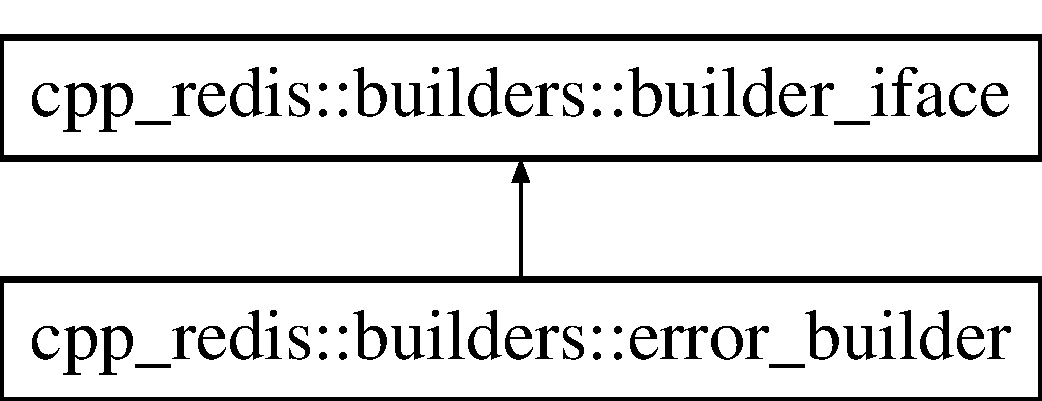
\includegraphics[height=2.000000cm]{classcpp__redis_1_1builders_1_1error__builder}
\end{center}
\end{figure}
\subsection*{Public Member Functions}
\begin{DoxyCompactItemize}
\item 
\mbox{\Hypertarget{classcpp__redis_1_1builders_1_1error__builder_abbc5e14b66702ec8b210fb1d288d2423}\label{classcpp__redis_1_1builders_1_1error__builder_abbc5e14b66702ec8b210fb1d288d2423}} 
\mbox{\hyperlink{classcpp__redis_1_1builders_1_1error__builder_abbc5e14b66702ec8b210fb1d288d2423}{error\+\_\+builder}} (void)=default
\begin{DoxyCompactList}\small\item\em ctor \end{DoxyCompactList}\item 
\mbox{\Hypertarget{classcpp__redis_1_1builders_1_1error__builder_a7650c178a457c57c2efb19e7ad256fe7}\label{classcpp__redis_1_1builders_1_1error__builder_a7650c178a457c57c2efb19e7ad256fe7}} 
\mbox{\hyperlink{classcpp__redis_1_1builders_1_1error__builder_a7650c178a457c57c2efb19e7ad256fe7}{$\sim$error\+\_\+builder}} (void)=default
\begin{DoxyCompactList}\small\item\em dtor \end{DoxyCompactList}\item 
\mbox{\Hypertarget{classcpp__redis_1_1builders_1_1error__builder_a2aee65fdc05abfacda73987e2cf60609}\label{classcpp__redis_1_1builders_1_1error__builder_a2aee65fdc05abfacda73987e2cf60609}} 
\mbox{\hyperlink{classcpp__redis_1_1builders_1_1error__builder_a2aee65fdc05abfacda73987e2cf60609}{error\+\_\+builder}} (const \mbox{\hyperlink{classcpp__redis_1_1builders_1_1error__builder}{error\+\_\+builder}} \&)=delete
\begin{DoxyCompactList}\small\item\em copy ctor \end{DoxyCompactList}\item 
\mbox{\Hypertarget{classcpp__redis_1_1builders_1_1error__builder_a0b1be51200ff84f17693ee888b03d505}\label{classcpp__redis_1_1builders_1_1error__builder_a0b1be51200ff84f17693ee888b03d505}} 
\mbox{\hyperlink{classcpp__redis_1_1builders_1_1error__builder}{error\+\_\+builder}} \& \mbox{\hyperlink{classcpp__redis_1_1builders_1_1error__builder_a0b1be51200ff84f17693ee888b03d505}{operator=}} (const \mbox{\hyperlink{classcpp__redis_1_1builders_1_1error__builder}{error\+\_\+builder}} \&)=delete
\begin{DoxyCompactList}\small\item\em assignment operator \end{DoxyCompactList}\item 
\mbox{\hyperlink{classcpp__redis_1_1builders_1_1builder__iface}{builder\+\_\+iface}} \& \mbox{\hyperlink{classcpp__redis_1_1builders_1_1error__builder_af5ac542be148d6f8500de79fa3164798}{operator$<$$<$}} (std\+::string \&data)
\item 
bool \mbox{\hyperlink{classcpp__redis_1_1builders_1_1error__builder_af3d67647f012d0a7378684e2f8258a6d}{reply\+\_\+ready}} (void) const
\item 
\mbox{\hyperlink{classcpp__redis_1_1reply}{reply}} \mbox{\hyperlink{classcpp__redis_1_1builders_1_1error__builder_ae2b68b7daad4d71b6780e47bdcc1e32b}{get\+\_\+reply}} (void) const
\item 
const std\+::string \& \mbox{\hyperlink{classcpp__redis_1_1builders_1_1error__builder_adeef989fb2f5e47e001783cfda48e341}{get\+\_\+error}} (void) const
\end{DoxyCompactItemize}


\subsection{Detailed Description}
builder to build redis error replies 

\subsection{Member Function Documentation}
\mbox{\Hypertarget{classcpp__redis_1_1builders_1_1error__builder_adeef989fb2f5e47e001783cfda48e341}\label{classcpp__redis_1_1builders_1_1error__builder_adeef989fb2f5e47e001783cfda48e341}} 
\index{cpp\+\_\+redis\+::builders\+::error\+\_\+builder@{cpp\+\_\+redis\+::builders\+::error\+\_\+builder}!get\+\_\+error@{get\+\_\+error}}
\index{get\+\_\+error@{get\+\_\+error}!cpp\+\_\+redis\+::builders\+::error\+\_\+builder@{cpp\+\_\+redis\+::builders\+::error\+\_\+builder}}
\subsubsection{\texorpdfstring{get\+\_\+error()}{get\_error()}}
{\footnotesize\ttfamily const std\+::string\& cpp\+\_\+redis\+::builders\+::error\+\_\+builder\+::get\+\_\+error (\begin{DoxyParamCaption}\item[{void}]{ }\end{DoxyParamCaption}) const}

\begin{DoxyReturn}{Returns}
the parsed error 
\end{DoxyReturn}
\mbox{\Hypertarget{classcpp__redis_1_1builders_1_1error__builder_ae2b68b7daad4d71b6780e47bdcc1e32b}\label{classcpp__redis_1_1builders_1_1error__builder_ae2b68b7daad4d71b6780e47bdcc1e32b}} 
\index{cpp\+\_\+redis\+::builders\+::error\+\_\+builder@{cpp\+\_\+redis\+::builders\+::error\+\_\+builder}!get\+\_\+reply@{get\+\_\+reply}}
\index{get\+\_\+reply@{get\+\_\+reply}!cpp\+\_\+redis\+::builders\+::error\+\_\+builder@{cpp\+\_\+redis\+::builders\+::error\+\_\+builder}}
\subsubsection{\texorpdfstring{get\+\_\+reply()}{get\_reply()}}
{\footnotesize\ttfamily \mbox{\hyperlink{classcpp__redis_1_1reply}{reply}} cpp\+\_\+redis\+::builders\+::error\+\_\+builder\+::get\+\_\+reply (\begin{DoxyParamCaption}\item[{void}]{ }\end{DoxyParamCaption}) const\hspace{0.3cm}{\ttfamily [virtual]}}

\begin{DoxyReturn}{Returns}
reply object 
\end{DoxyReturn}


Implements \mbox{\hyperlink{classcpp__redis_1_1builders_1_1builder__iface_afd2ff2c2371c2a486116543b638b9413}{cpp\+\_\+redis\+::builders\+::builder\+\_\+iface}}.

\mbox{\Hypertarget{classcpp__redis_1_1builders_1_1error__builder_af5ac542be148d6f8500de79fa3164798}\label{classcpp__redis_1_1builders_1_1error__builder_af5ac542be148d6f8500de79fa3164798}} 
\index{cpp\+\_\+redis\+::builders\+::error\+\_\+builder@{cpp\+\_\+redis\+::builders\+::error\+\_\+builder}!operator$<$$<$@{operator$<$$<$}}
\index{operator$<$$<$@{operator$<$$<$}!cpp\+\_\+redis\+::builders\+::error\+\_\+builder@{cpp\+\_\+redis\+::builders\+::error\+\_\+builder}}
\subsubsection{\texorpdfstring{operator$<$$<$()}{operator<<()}}
{\footnotesize\ttfamily \mbox{\hyperlink{classcpp__redis_1_1builders_1_1builder__iface}{builder\+\_\+iface}}\& cpp\+\_\+redis\+::builders\+::error\+\_\+builder\+::operator$<$$<$ (\begin{DoxyParamCaption}\item[{std\+::string \&}]{data }\end{DoxyParamCaption})\hspace{0.3cm}{\ttfamily [virtual]}}

take data as parameter which is consumed to build the reply every bytes used to build the reply must be removed from the buffer passed as parameter


\begin{DoxyParams}{Parameters}
{\em data} & data to be consumed \\
\hline
\end{DoxyParams}
\begin{DoxyReturn}{Returns}
current instance 
\end{DoxyReturn}


Implements \mbox{\hyperlink{classcpp__redis_1_1builders_1_1builder__iface_a9892bbc9c887c31c2742dad4476e2fa6}{cpp\+\_\+redis\+::builders\+::builder\+\_\+iface}}.

\mbox{\Hypertarget{classcpp__redis_1_1builders_1_1error__builder_af3d67647f012d0a7378684e2f8258a6d}\label{classcpp__redis_1_1builders_1_1error__builder_af3d67647f012d0a7378684e2f8258a6d}} 
\index{cpp\+\_\+redis\+::builders\+::error\+\_\+builder@{cpp\+\_\+redis\+::builders\+::error\+\_\+builder}!reply\+\_\+ready@{reply\+\_\+ready}}
\index{reply\+\_\+ready@{reply\+\_\+ready}!cpp\+\_\+redis\+::builders\+::error\+\_\+builder@{cpp\+\_\+redis\+::builders\+::error\+\_\+builder}}
\subsubsection{\texorpdfstring{reply\+\_\+ready()}{reply\_ready()}}
{\footnotesize\ttfamily bool cpp\+\_\+redis\+::builders\+::error\+\_\+builder\+::reply\+\_\+ready (\begin{DoxyParamCaption}\item[{void}]{ }\end{DoxyParamCaption}) const\hspace{0.3cm}{\ttfamily [virtual]}}

\begin{DoxyReturn}{Returns}
whether the reply could be built 
\end{DoxyReturn}


Implements \mbox{\hyperlink{classcpp__redis_1_1builders_1_1builder__iface_a40db9a31d4ea1771777e74146d31e12d}{cpp\+\_\+redis\+::builders\+::builder\+\_\+iface}}.



The documentation for this class was generated from the following file\+:\begin{DoxyCompactItemize}
\item 
includes/cpp\+\_\+redis/builders/error\+\_\+builder.\+hpp\end{DoxyCompactItemize}

\hypertarget{structcpp__redis_1_1helpers_1_1front}{}\section{cpp\+\_\+redis\+:\+:helpers\+:\+:front$<$ T, Ts $>$ Struct Template Reference}
\label{structcpp__redis_1_1helpers_1_1front}\index{cpp\+\_\+redis\+::helpers\+::front$<$ T, Ts $>$@{cpp\+\_\+redis\+::helpers\+::front$<$ T, Ts $>$}}


{\ttfamily \#include $<$variadic\+\_\+template.\+hpp$>$}

\subsection*{Public Types}
\begin{DoxyCompactItemize}
\item 
using \hyperlink{structcpp__redis_1_1helpers_1_1front_a23178392c9417cc5ada75205931d1768}{type} = T
\end{DoxyCompactItemize}


\subsection{Detailed Description}
\subsubsection*{template$<$typename T, typename... Ts$>$\newline
struct cpp\+\_\+redis\+::helpers\+::front$<$ T, Ts $>$}

type traits to return front element of a variadic list 

\subsection{Member Typedef Documentation}
\mbox{\Hypertarget{structcpp__redis_1_1helpers_1_1front_a23178392c9417cc5ada75205931d1768}\label{structcpp__redis_1_1helpers_1_1front_a23178392c9417cc5ada75205931d1768}} 
\index{cpp\+\_\+redis\+::helpers\+::front@{cpp\+\_\+redis\+::helpers\+::front}!type@{type}}
\index{type@{type}!cpp\+\_\+redis\+::helpers\+::front@{cpp\+\_\+redis\+::helpers\+::front}}
\subsubsection{\texorpdfstring{type}{type}}
{\footnotesize\ttfamily template$<$typename T , typename... Ts$>$ \\
using \hyperlink{structcpp__redis_1_1helpers_1_1front}{cpp\+\_\+redis\+::helpers\+::front}$<$ T, Ts $>$\+::\hyperlink{structcpp__redis_1_1helpers_1_1front_a23178392c9417cc5ada75205931d1768}{type} =  T}

front type of variadic list 

The documentation for this struct was generated from the following file\+:\begin{DoxyCompactItemize}
\item 
includes/cpp\+\_\+redis/helpers/variadic\+\_\+template.\+hpp\end{DoxyCompactItemize}

\hypertarget{classcpp__redis_1_1builders_1_1integer__builder}{}\section{cpp\+\_\+redis\+:\+:builders\+:\+:integer\+\_\+builder Class Reference}
\label{classcpp__redis_1_1builders_1_1integer__builder}\index{cpp\+\_\+redis\+::builders\+::integer\+\_\+builder@{cpp\+\_\+redis\+::builders\+::integer\+\_\+builder}}


{\ttfamily \#include $<$integer\+\_\+builder.\+hpp$>$}

Inheritance diagram for cpp\+\_\+redis\+:\+:builders\+:\+:integer\+\_\+builder\+:\begin{figure}[H]
\begin{center}
\leavevmode
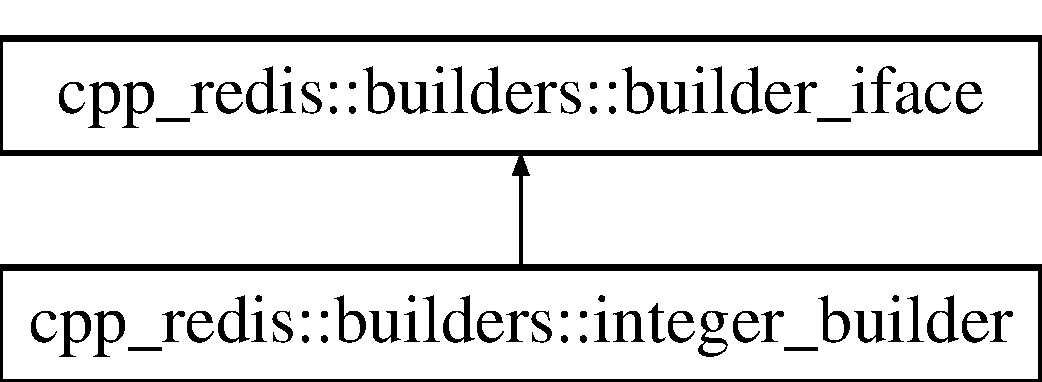
\includegraphics[height=2.000000cm]{classcpp__redis_1_1builders_1_1integer__builder}
\end{center}
\end{figure}
\subsection*{Public Member Functions}
\begin{DoxyCompactItemize}
\item 
\hyperlink{classcpp__redis_1_1builders_1_1integer__builder_a9ff2d3d27da0fb8b98fc4a0ea255fece}{integer\+\_\+builder} (void)
\begin{DoxyCompactList}\small\item\em ctor \end{DoxyCompactList}\item 
\hyperlink{classcpp__redis_1_1builders_1_1integer__builder_ab2b797dd89b1bdec50f8ccf07633162f}{$\sim$integer\+\_\+builder} (void)=default
\begin{DoxyCompactList}\small\item\em dtor \end{DoxyCompactList}\item 
\hyperlink{classcpp__redis_1_1builders_1_1integer__builder_ab451b7fe5de8cf6f618cf9be1569aa41}{integer\+\_\+builder} (const \hyperlink{classcpp__redis_1_1builders_1_1integer__builder}{integer\+\_\+builder} \&)=delete
\begin{DoxyCompactList}\small\item\em copy ctor \end{DoxyCompactList}\item 
\hyperlink{classcpp__redis_1_1builders_1_1integer__builder}{integer\+\_\+builder} \& \hyperlink{classcpp__redis_1_1builders_1_1integer__builder_a259905e8a34765d6ff9d2dd64f444b54}{operator=} (const \hyperlink{classcpp__redis_1_1builders_1_1integer__builder}{integer\+\_\+builder} \&)=delete
\begin{DoxyCompactList}\small\item\em assignment operator \end{DoxyCompactList}\item 
\hyperlink{classcpp__redis_1_1builders_1_1builder__iface}{builder\+\_\+iface} \& \hyperlink{classcpp__redis_1_1builders_1_1integer__builder_ae29f074134f7269db7f947b0fcbe312e}{operator$<$$<$} (std\+::string \&data)
\item 
bool \hyperlink{classcpp__redis_1_1builders_1_1integer__builder_a4893dc36d06d75094bb4fe3fbc826966}{reply\+\_\+ready} (void) const
\item 
\hyperlink{classcpp__redis_1_1reply}{reply} \hyperlink{classcpp__redis_1_1builders_1_1integer__builder_a25221763ba6f8b740458c673945208e0}{get\+\_\+reply} (void) const
\item 
int64\+\_\+t \hyperlink{classcpp__redis_1_1builders_1_1integer__builder_af68431c4c81242c1930b3b4feb2028e5}{get\+\_\+integer} (void) const
\end{DoxyCompactItemize}
\subsection*{Private Attributes}
\begin{DoxyCompactItemize}
\item 
int64\+\_\+t \hyperlink{classcpp__redis_1_1builders_1_1integer__builder_af3b37f54856e09f45fdd8c9f0443d8a7}{m\+\_\+nbr}
\item 
int64\+\_\+t \hyperlink{classcpp__redis_1_1builders_1_1integer__builder_ae1c6d8b48c44f022e9dea4718a4ae25f}{m\+\_\+negative\+\_\+multiplicator}
\item 
bool \hyperlink{classcpp__redis_1_1builders_1_1integer__builder_ab2e676e8e881987fe56847bf992a7a09}{m\+\_\+reply\+\_\+ready}
\item 
\hyperlink{classcpp__redis_1_1reply}{reply} \hyperlink{classcpp__redis_1_1builders_1_1integer__builder_a0c9b1dc87ca9f0cb9576283fe5482548}{m\+\_\+reply}
\end{DoxyCompactItemize}


\subsection{Detailed Description}
builder to build redis integer replies 

\subsection{Constructor \& Destructor Documentation}
\mbox{\Hypertarget{classcpp__redis_1_1builders_1_1integer__builder_a9ff2d3d27da0fb8b98fc4a0ea255fece}\label{classcpp__redis_1_1builders_1_1integer__builder_a9ff2d3d27da0fb8b98fc4a0ea255fece}} 
\index{cpp\+\_\+redis\+::builders\+::integer\+\_\+builder@{cpp\+\_\+redis\+::builders\+::integer\+\_\+builder}!integer\+\_\+builder@{integer\+\_\+builder}}
\index{integer\+\_\+builder@{integer\+\_\+builder}!cpp\+\_\+redis\+::builders\+::integer\+\_\+builder@{cpp\+\_\+redis\+::builders\+::integer\+\_\+builder}}
\subsubsection{\texorpdfstring{integer\+\_\+builder()}{integer\_builder()}\hspace{0.1cm}{\footnotesize\ttfamily [1/2]}}
{\footnotesize\ttfamily cpp\+\_\+redis\+::builders\+::integer\+\_\+builder\+::integer\+\_\+builder (\begin{DoxyParamCaption}\item[{void}]{ }\end{DoxyParamCaption})}



ctor 

\mbox{\Hypertarget{classcpp__redis_1_1builders_1_1integer__builder_ab2b797dd89b1bdec50f8ccf07633162f}\label{classcpp__redis_1_1builders_1_1integer__builder_ab2b797dd89b1bdec50f8ccf07633162f}} 
\index{cpp\+\_\+redis\+::builders\+::integer\+\_\+builder@{cpp\+\_\+redis\+::builders\+::integer\+\_\+builder}!````~integer\+\_\+builder@{$\sim$integer\+\_\+builder}}
\index{````~integer\+\_\+builder@{$\sim$integer\+\_\+builder}!cpp\+\_\+redis\+::builders\+::integer\+\_\+builder@{cpp\+\_\+redis\+::builders\+::integer\+\_\+builder}}
\subsubsection{\texorpdfstring{$\sim$integer\+\_\+builder()}{~integer\_builder()}}
{\footnotesize\ttfamily cpp\+\_\+redis\+::builders\+::integer\+\_\+builder\+::$\sim$integer\+\_\+builder (\begin{DoxyParamCaption}\item[{void}]{ }\end{DoxyParamCaption})\hspace{0.3cm}{\ttfamily [default]}}



dtor 

\mbox{\Hypertarget{classcpp__redis_1_1builders_1_1integer__builder_ab451b7fe5de8cf6f618cf9be1569aa41}\label{classcpp__redis_1_1builders_1_1integer__builder_ab451b7fe5de8cf6f618cf9be1569aa41}} 
\index{cpp\+\_\+redis\+::builders\+::integer\+\_\+builder@{cpp\+\_\+redis\+::builders\+::integer\+\_\+builder}!integer\+\_\+builder@{integer\+\_\+builder}}
\index{integer\+\_\+builder@{integer\+\_\+builder}!cpp\+\_\+redis\+::builders\+::integer\+\_\+builder@{cpp\+\_\+redis\+::builders\+::integer\+\_\+builder}}
\subsubsection{\texorpdfstring{integer\+\_\+builder()}{integer\_builder()}\hspace{0.1cm}{\footnotesize\ttfamily [2/2]}}
{\footnotesize\ttfamily cpp\+\_\+redis\+::builders\+::integer\+\_\+builder\+::integer\+\_\+builder (\begin{DoxyParamCaption}\item[{const \hyperlink{classcpp__redis_1_1builders_1_1integer__builder}{integer\+\_\+builder} \&}]{ }\end{DoxyParamCaption})\hspace{0.3cm}{\ttfamily [delete]}}



copy ctor 



\subsection{Member Function Documentation}
\mbox{\Hypertarget{classcpp__redis_1_1builders_1_1integer__builder_af68431c4c81242c1930b3b4feb2028e5}\label{classcpp__redis_1_1builders_1_1integer__builder_af68431c4c81242c1930b3b4feb2028e5}} 
\index{cpp\+\_\+redis\+::builders\+::integer\+\_\+builder@{cpp\+\_\+redis\+::builders\+::integer\+\_\+builder}!get\+\_\+integer@{get\+\_\+integer}}
\index{get\+\_\+integer@{get\+\_\+integer}!cpp\+\_\+redis\+::builders\+::integer\+\_\+builder@{cpp\+\_\+redis\+::builders\+::integer\+\_\+builder}}
\subsubsection{\texorpdfstring{get\+\_\+integer()}{get\_integer()}}
{\footnotesize\ttfamily int64\+\_\+t cpp\+\_\+redis\+::builders\+::integer\+\_\+builder\+::get\+\_\+integer (\begin{DoxyParamCaption}\item[{void}]{ }\end{DoxyParamCaption}) const}

\begin{DoxyReturn}{Returns}
the parsed integer 
\end{DoxyReturn}
\mbox{\Hypertarget{classcpp__redis_1_1builders_1_1integer__builder_a25221763ba6f8b740458c673945208e0}\label{classcpp__redis_1_1builders_1_1integer__builder_a25221763ba6f8b740458c673945208e0}} 
\index{cpp\+\_\+redis\+::builders\+::integer\+\_\+builder@{cpp\+\_\+redis\+::builders\+::integer\+\_\+builder}!get\+\_\+reply@{get\+\_\+reply}}
\index{get\+\_\+reply@{get\+\_\+reply}!cpp\+\_\+redis\+::builders\+::integer\+\_\+builder@{cpp\+\_\+redis\+::builders\+::integer\+\_\+builder}}
\subsubsection{\texorpdfstring{get\+\_\+reply()}{get\_reply()}}
{\footnotesize\ttfamily \hyperlink{classcpp__redis_1_1reply}{reply} cpp\+\_\+redis\+::builders\+::integer\+\_\+builder\+::get\+\_\+reply (\begin{DoxyParamCaption}\item[{void}]{ }\end{DoxyParamCaption}) const\hspace{0.3cm}{\ttfamily [virtual]}}

\begin{DoxyReturn}{Returns}
reply object 
\end{DoxyReturn}


Implements \hyperlink{classcpp__redis_1_1builders_1_1builder__iface_afd2ff2c2371c2a486116543b638b9413}{cpp\+\_\+redis\+::builders\+::builder\+\_\+iface}.

\mbox{\Hypertarget{classcpp__redis_1_1builders_1_1integer__builder_ae29f074134f7269db7f947b0fcbe312e}\label{classcpp__redis_1_1builders_1_1integer__builder_ae29f074134f7269db7f947b0fcbe312e}} 
\index{cpp\+\_\+redis\+::builders\+::integer\+\_\+builder@{cpp\+\_\+redis\+::builders\+::integer\+\_\+builder}!operator$<$$<$@{operator$<$$<$}}
\index{operator$<$$<$@{operator$<$$<$}!cpp\+\_\+redis\+::builders\+::integer\+\_\+builder@{cpp\+\_\+redis\+::builders\+::integer\+\_\+builder}}
\subsubsection{\texorpdfstring{operator$<$$<$()}{operator<<()}}
{\footnotesize\ttfamily \hyperlink{classcpp__redis_1_1builders_1_1builder__iface}{builder\+\_\+iface}\& cpp\+\_\+redis\+::builders\+::integer\+\_\+builder\+::operator$<$$<$ (\begin{DoxyParamCaption}\item[{std\+::string \&}]{data }\end{DoxyParamCaption})\hspace{0.3cm}{\ttfamily [virtual]}}

take data as parameter which is consumed to build the reply every bytes used to build the reply must be removed from the buffer passed as parameter


\begin{DoxyParams}{Parameters}
{\em data} & data to be consumed \\
\hline
\end{DoxyParams}
\begin{DoxyReturn}{Returns}
current instance 
\end{DoxyReturn}


Implements \hyperlink{classcpp__redis_1_1builders_1_1builder__iface_a9892bbc9c887c31c2742dad4476e2fa6}{cpp\+\_\+redis\+::builders\+::builder\+\_\+iface}.

\mbox{\Hypertarget{classcpp__redis_1_1builders_1_1integer__builder_a259905e8a34765d6ff9d2dd64f444b54}\label{classcpp__redis_1_1builders_1_1integer__builder_a259905e8a34765d6ff9d2dd64f444b54}} 
\index{cpp\+\_\+redis\+::builders\+::integer\+\_\+builder@{cpp\+\_\+redis\+::builders\+::integer\+\_\+builder}!operator=@{operator=}}
\index{operator=@{operator=}!cpp\+\_\+redis\+::builders\+::integer\+\_\+builder@{cpp\+\_\+redis\+::builders\+::integer\+\_\+builder}}
\subsubsection{\texorpdfstring{operator=()}{operator=()}}
{\footnotesize\ttfamily \hyperlink{classcpp__redis_1_1builders_1_1integer__builder}{integer\+\_\+builder}\& cpp\+\_\+redis\+::builders\+::integer\+\_\+builder\+::operator= (\begin{DoxyParamCaption}\item[{const \hyperlink{classcpp__redis_1_1builders_1_1integer__builder}{integer\+\_\+builder} \&}]{ }\end{DoxyParamCaption})\hspace{0.3cm}{\ttfamily [delete]}}



assignment operator 

\mbox{\Hypertarget{classcpp__redis_1_1builders_1_1integer__builder_a4893dc36d06d75094bb4fe3fbc826966}\label{classcpp__redis_1_1builders_1_1integer__builder_a4893dc36d06d75094bb4fe3fbc826966}} 
\index{cpp\+\_\+redis\+::builders\+::integer\+\_\+builder@{cpp\+\_\+redis\+::builders\+::integer\+\_\+builder}!reply\+\_\+ready@{reply\+\_\+ready}}
\index{reply\+\_\+ready@{reply\+\_\+ready}!cpp\+\_\+redis\+::builders\+::integer\+\_\+builder@{cpp\+\_\+redis\+::builders\+::integer\+\_\+builder}}
\subsubsection{\texorpdfstring{reply\+\_\+ready()}{reply\_ready()}}
{\footnotesize\ttfamily bool cpp\+\_\+redis\+::builders\+::integer\+\_\+builder\+::reply\+\_\+ready (\begin{DoxyParamCaption}\item[{void}]{ }\end{DoxyParamCaption}) const\hspace{0.3cm}{\ttfamily [virtual]}}

\begin{DoxyReturn}{Returns}
whether the reply could be built 
\end{DoxyReturn}


Implements \hyperlink{classcpp__redis_1_1builders_1_1builder__iface_a40db9a31d4ea1771777e74146d31e12d}{cpp\+\_\+redis\+::builders\+::builder\+\_\+iface}.



\subsection{Member Data Documentation}
\mbox{\Hypertarget{classcpp__redis_1_1builders_1_1integer__builder_af3b37f54856e09f45fdd8c9f0443d8a7}\label{classcpp__redis_1_1builders_1_1integer__builder_af3b37f54856e09f45fdd8c9f0443d8a7}} 
\index{cpp\+\_\+redis\+::builders\+::integer\+\_\+builder@{cpp\+\_\+redis\+::builders\+::integer\+\_\+builder}!m\+\_\+nbr@{m\+\_\+nbr}}
\index{m\+\_\+nbr@{m\+\_\+nbr}!cpp\+\_\+redis\+::builders\+::integer\+\_\+builder@{cpp\+\_\+redis\+::builders\+::integer\+\_\+builder}}
\subsubsection{\texorpdfstring{m\+\_\+nbr}{m\_nbr}}
{\footnotesize\ttfamily int64\+\_\+t cpp\+\_\+redis\+::builders\+::integer\+\_\+builder\+::m\+\_\+nbr\hspace{0.3cm}{\ttfamily [private]}}

parsed number \mbox{\Hypertarget{classcpp__redis_1_1builders_1_1integer__builder_ae1c6d8b48c44f022e9dea4718a4ae25f}\label{classcpp__redis_1_1builders_1_1integer__builder_ae1c6d8b48c44f022e9dea4718a4ae25f}} 
\index{cpp\+\_\+redis\+::builders\+::integer\+\_\+builder@{cpp\+\_\+redis\+::builders\+::integer\+\_\+builder}!m\+\_\+negative\+\_\+multiplicator@{m\+\_\+negative\+\_\+multiplicator}}
\index{m\+\_\+negative\+\_\+multiplicator@{m\+\_\+negative\+\_\+multiplicator}!cpp\+\_\+redis\+::builders\+::integer\+\_\+builder@{cpp\+\_\+redis\+::builders\+::integer\+\_\+builder}}
\subsubsection{\texorpdfstring{m\+\_\+negative\+\_\+multiplicator}{m\_negative\_multiplicator}}
{\footnotesize\ttfamily int64\+\_\+t cpp\+\_\+redis\+::builders\+::integer\+\_\+builder\+::m\+\_\+negative\+\_\+multiplicator\hspace{0.3cm}{\ttfamily [private]}}

-\/1 for negative number, 1 otherwise \mbox{\Hypertarget{classcpp__redis_1_1builders_1_1integer__builder_a0c9b1dc87ca9f0cb9576283fe5482548}\label{classcpp__redis_1_1builders_1_1integer__builder_a0c9b1dc87ca9f0cb9576283fe5482548}} 
\index{cpp\+\_\+redis\+::builders\+::integer\+\_\+builder@{cpp\+\_\+redis\+::builders\+::integer\+\_\+builder}!m\+\_\+reply@{m\+\_\+reply}}
\index{m\+\_\+reply@{m\+\_\+reply}!cpp\+\_\+redis\+::builders\+::integer\+\_\+builder@{cpp\+\_\+redis\+::builders\+::integer\+\_\+builder}}
\subsubsection{\texorpdfstring{m\+\_\+reply}{m\_reply}}
{\footnotesize\ttfamily \hyperlink{classcpp__redis_1_1reply}{reply} cpp\+\_\+redis\+::builders\+::integer\+\_\+builder\+::m\+\_\+reply\hspace{0.3cm}{\ttfamily [private]}}

reply to be built \mbox{\Hypertarget{classcpp__redis_1_1builders_1_1integer__builder_ab2e676e8e881987fe56847bf992a7a09}\label{classcpp__redis_1_1builders_1_1integer__builder_ab2e676e8e881987fe56847bf992a7a09}} 
\index{cpp\+\_\+redis\+::builders\+::integer\+\_\+builder@{cpp\+\_\+redis\+::builders\+::integer\+\_\+builder}!m\+\_\+reply\+\_\+ready@{m\+\_\+reply\+\_\+ready}}
\index{m\+\_\+reply\+\_\+ready@{m\+\_\+reply\+\_\+ready}!cpp\+\_\+redis\+::builders\+::integer\+\_\+builder@{cpp\+\_\+redis\+::builders\+::integer\+\_\+builder}}
\subsubsection{\texorpdfstring{m\+\_\+reply\+\_\+ready}{m\_reply\_ready}}
{\footnotesize\ttfamily bool cpp\+\_\+redis\+::builders\+::integer\+\_\+builder\+::m\+\_\+reply\+\_\+ready\hspace{0.3cm}{\ttfamily [private]}}

whether the reply is ready or not 

The documentation for this class was generated from the following file\+:\begin{DoxyCompactItemize}
\item 
includes/cpp\+\_\+redis/builders/\hyperlink{integer__builder_8hpp}{integer\+\_\+builder.\+hpp}\end{DoxyCompactItemize}

\hypertarget{structcpp__redis_1_1helpers_1_1is__different__types}{}\section{cpp\+\_\+redis\+:\+:helpers\+:\+:is\+\_\+different\+\_\+types$<$ T, Args $>$ Struct Template Reference}
\label{structcpp__redis_1_1helpers_1_1is__different__types}\index{cpp\+\_\+redis\+::helpers\+::is\+\_\+different\+\_\+types$<$ T, Args $>$@{cpp\+\_\+redis\+::helpers\+::is\+\_\+different\+\_\+types$<$ T, Args $>$}}


{\ttfamily \#include $<$variadic\+\_\+template.\+hpp$>$}

\subsection*{Static Public Attributes}
\begin{DoxyCompactItemize}
\item 
static constexpr bool \hyperlink{structcpp__redis_1_1helpers_1_1is__different__types_a07dadd8ff3c8024734f231aaf1555626}{value}
\end{DoxyCompactItemize}


\subsection{Detailed Description}
\subsubsection*{template$<$typename T, typename... Args$>$\newline
struct cpp\+\_\+redis\+::helpers\+::is\+\_\+different\+\_\+types$<$ T, Args $>$}

type traits to check if type is not present in variadic list 

\subsection{Member Data Documentation}
\mbox{\Hypertarget{structcpp__redis_1_1helpers_1_1is__different__types_a07dadd8ff3c8024734f231aaf1555626}\label{structcpp__redis_1_1helpers_1_1is__different__types_a07dadd8ff3c8024734f231aaf1555626}} 
\index{cpp\+\_\+redis\+::helpers\+::is\+\_\+different\+\_\+types@{cpp\+\_\+redis\+::helpers\+::is\+\_\+different\+\_\+types}!value@{value}}
\index{value@{value}!cpp\+\_\+redis\+::helpers\+::is\+\_\+different\+\_\+types@{cpp\+\_\+redis\+::helpers\+::is\+\_\+different\+\_\+types}}
\subsubsection{\texorpdfstring{value}{value}}
{\footnotesize\ttfamily template$<$typename T , typename... Args$>$ \\
constexpr bool \hyperlink{structcpp__redis_1_1helpers_1_1is__different__types}{cpp\+\_\+redis\+::helpers\+::is\+\_\+different\+\_\+types}$<$ T, Args $>$\+::value\hspace{0.3cm}{\ttfamily [static]}}

{\bfseries Initial value\+:}
\begin{DoxyCode}
= is\_type\_present<T, Args...>\hyperlink{structcpp__redis_1_1helpers_1_1is__different__types_a07dadd8ff3c8024734f231aaf1555626}{::value}
                                  ? false
                                  : is\_different\_types<Args...>\hyperlink{structcpp__redis_1_1helpers_1_1is__different__types_a07dadd8ff3c8024734f231aaf1555626}{::value}
\end{DoxyCode}


The documentation for this struct was generated from the following file\+:\begin{DoxyCompactItemize}
\item 
includes/cpp\+\_\+redis/helpers/\hyperlink{variadic__template_8hpp}{variadic\+\_\+template.\+hpp}\end{DoxyCompactItemize}

\hypertarget{structcpp__redis_1_1helpers_1_1is__different__types_3_01_t1_01_4}{}\section{cpp\+\_\+redis\+:\+:helpers\+:\+:is\+\_\+different\+\_\+types$<$ T1 $>$ Struct Template Reference}
\label{structcpp__redis_1_1helpers_1_1is__different__types_3_01_t1_01_4}\index{cpp\+\_\+redis\+::helpers\+::is\+\_\+different\+\_\+types$<$ T1 $>$@{cpp\+\_\+redis\+::helpers\+::is\+\_\+different\+\_\+types$<$ T1 $>$}}


{\ttfamily \#include $<$variadic\+\_\+template.\+hpp$>$}

\subsection*{Static Public Attributes}
\begin{DoxyCompactItemize}
\item 
static constexpr bool \mbox{\hyperlink{structcpp__redis_1_1helpers_1_1is__different__types_3_01_t1_01_4_ae05b9b4af6846340ac66fcf64a622397}{value}} = true
\end{DoxyCompactItemize}


\subsection{Detailed Description}
\subsubsection*{template$<$typename T1$>$\newline
struct cpp\+\_\+redis\+::helpers\+::is\+\_\+different\+\_\+types$<$ T1 $>$}

type traits to check if type is not present in variadic list 

\subsection{Member Data Documentation}
\mbox{\Hypertarget{structcpp__redis_1_1helpers_1_1is__different__types_3_01_t1_01_4_ae05b9b4af6846340ac66fcf64a622397}\label{structcpp__redis_1_1helpers_1_1is__different__types_3_01_t1_01_4_ae05b9b4af6846340ac66fcf64a622397}} 
\index{cpp\+\_\+redis\+::helpers\+::is\+\_\+different\+\_\+types$<$ T1 $>$@{cpp\+\_\+redis\+::helpers\+::is\+\_\+different\+\_\+types$<$ T1 $>$}!value@{value}}
\index{value@{value}!cpp\+\_\+redis\+::helpers\+::is\+\_\+different\+\_\+types$<$ T1 $>$@{cpp\+\_\+redis\+::helpers\+::is\+\_\+different\+\_\+types$<$ T1 $>$}}
\subsubsection{\texorpdfstring{value}{value}}
{\footnotesize\ttfamily template$<$typename T1 $>$ \\
constexpr bool \mbox{\hyperlink{structcpp__redis_1_1helpers_1_1is__different__types}{cpp\+\_\+redis\+::helpers\+::is\+\_\+different\+\_\+types}}$<$ T1 $>$\+::value = true\hspace{0.3cm}{\ttfamily [static]}}

true 

The documentation for this struct was generated from the following file\+:\begin{DoxyCompactItemize}
\item 
includes/cpp\+\_\+redis/helpers/variadic\+\_\+template.\+hpp\end{DoxyCompactItemize}

\hypertarget{structcpp__redis_1_1helpers_1_1is__type__present}{}\section{cpp\+\_\+redis\+:\+:helpers\+:\+:is\+\_\+type\+\_\+present$<$ T1, T2, Ts $>$ Struct Template Reference}
\label{structcpp__redis_1_1helpers_1_1is__type__present}\index{cpp\+\_\+redis\+::helpers\+::is\+\_\+type\+\_\+present$<$ T1, T2, Ts $>$@{cpp\+\_\+redis\+::helpers\+::is\+\_\+type\+\_\+present$<$ T1, T2, Ts $>$}}


{\ttfamily \#include $<$variadic\+\_\+template.\+hpp$>$}

\subsection*{Static Public Attributes}
\begin{DoxyCompactItemize}
\item 
static constexpr bool \hyperlink{structcpp__redis_1_1helpers_1_1is__type__present_a7b5e8d970ba974a9b58cbc440983c25c}{value}
\end{DoxyCompactItemize}


\subsection{Detailed Description}
\subsubsection*{template$<$typename T1, typename T2, typename... Ts$>$\newline
struct cpp\+\_\+redis\+::helpers\+::is\+\_\+type\+\_\+present$<$ T1, T2, Ts $>$}

type traits to check if type is present in variadic list 

\subsection{Member Data Documentation}
\mbox{\Hypertarget{structcpp__redis_1_1helpers_1_1is__type__present_a7b5e8d970ba974a9b58cbc440983c25c}\label{structcpp__redis_1_1helpers_1_1is__type__present_a7b5e8d970ba974a9b58cbc440983c25c}} 
\index{cpp\+\_\+redis\+::helpers\+::is\+\_\+type\+\_\+present@{cpp\+\_\+redis\+::helpers\+::is\+\_\+type\+\_\+present}!value@{value}}
\index{value@{value}!cpp\+\_\+redis\+::helpers\+::is\+\_\+type\+\_\+present@{cpp\+\_\+redis\+::helpers\+::is\+\_\+type\+\_\+present}}
\subsubsection{\texorpdfstring{value}{value}}
{\footnotesize\ttfamily template$<$typename T1 , typename T2 , typename... Ts$>$ \\
constexpr bool \hyperlink{structcpp__redis_1_1helpers_1_1is__type__present}{cpp\+\_\+redis\+::helpers\+::is\+\_\+type\+\_\+present}$<$ T1, T2, Ts $>$\+::value\hspace{0.3cm}{\ttfamily [static]}}

{\bfseries Initial value\+:}
\begin{DoxyCode}
= std::is\_same<T1, T2>::value
                                  ? true
                                  : is\_type\_present<T1, Ts...>\hyperlink{structcpp__redis_1_1helpers_1_1is__type__present_a7b5e8d970ba974a9b58cbc440983c25c}{::value}
\end{DoxyCode}


The documentation for this struct was generated from the following file\+:\begin{DoxyCompactItemize}
\item 
includes/cpp\+\_\+redis/helpers/\hyperlink{variadic__template_8hpp}{variadic\+\_\+template.\+hpp}\end{DoxyCompactItemize}

\hypertarget{structcpp__redis_1_1helpers_1_1is__type__present_3_01_t1_00_01_t2_01_4}{}\section{cpp\+\_\+redis\+:\+:helpers\+:\+:is\+\_\+type\+\_\+present$<$ T1, T2 $>$ Struct Template Reference}
\label{structcpp__redis_1_1helpers_1_1is__type__present_3_01_t1_00_01_t2_01_4}\index{cpp\+\_\+redis\+::helpers\+::is\+\_\+type\+\_\+present$<$ T1, T2 $>$@{cpp\+\_\+redis\+::helpers\+::is\+\_\+type\+\_\+present$<$ T1, T2 $>$}}


{\ttfamily \#include $<$variadic\+\_\+template.\+hpp$>$}

\subsection*{Static Public Attributes}
\begin{DoxyCompactItemize}
\item 
static constexpr bool \hyperlink{structcpp__redis_1_1helpers_1_1is__type__present_3_01_t1_00_01_t2_01_4_a1dbf43b76ba407caf9bfb35ffdbe55ad}{value} = std\+::is\+\_\+same$<$T1, T2$>$\+::value
\end{DoxyCompactItemize}


\subsection{Detailed Description}
\subsubsection*{template$<$typename T1, typename T2$>$\newline
struct cpp\+\_\+redis\+::helpers\+::is\+\_\+type\+\_\+present$<$ T1, T2 $>$}

type traits to check if type is present in variadic list 

\subsection{Member Data Documentation}
\mbox{\Hypertarget{structcpp__redis_1_1helpers_1_1is__type__present_3_01_t1_00_01_t2_01_4_a1dbf43b76ba407caf9bfb35ffdbe55ad}\label{structcpp__redis_1_1helpers_1_1is__type__present_3_01_t1_00_01_t2_01_4_a1dbf43b76ba407caf9bfb35ffdbe55ad}} 
\index{cpp\+\_\+redis\+::helpers\+::is\+\_\+type\+\_\+present$<$ T1, T2 $>$@{cpp\+\_\+redis\+::helpers\+::is\+\_\+type\+\_\+present$<$ T1, T2 $>$}!value@{value}}
\index{value@{value}!cpp\+\_\+redis\+::helpers\+::is\+\_\+type\+\_\+present$<$ T1, T2 $>$@{cpp\+\_\+redis\+::helpers\+::is\+\_\+type\+\_\+present$<$ T1, T2 $>$}}
\subsubsection{\texorpdfstring{value}{value}}
{\footnotesize\ttfamily template$<$typename T1 , typename T2 $>$ \\
constexpr bool \hyperlink{structcpp__redis_1_1helpers_1_1is__type__present}{cpp\+\_\+redis\+::helpers\+::is\+\_\+type\+\_\+present}$<$ T1, T2 $>$\+::value = std\+::is\+\_\+same$<$T1, T2$>$\+::value\hspace{0.3cm}{\ttfamily [static]}}

true if T1 and T2 are the same false otherwise 

The documentation for this struct was generated from the following file\+:\begin{DoxyCompactItemize}
\item 
includes/cpp\+\_\+redis/helpers/variadic\+\_\+template.\+hpp\end{DoxyCompactItemize}

\hypertarget{classcpp__redis_1_1logger}{}\section{cpp\+\_\+redis\+:\+:logger Class Reference}
\label{classcpp__redis_1_1logger}\index{cpp\+\_\+redis\+::logger@{cpp\+\_\+redis\+::logger}}


{\ttfamily \#include $<$logger.\+hpp$>$}

Inheritance diagram for cpp\+\_\+redis\+:\+:logger\+:\begin{figure}[H]
\begin{center}
\leavevmode
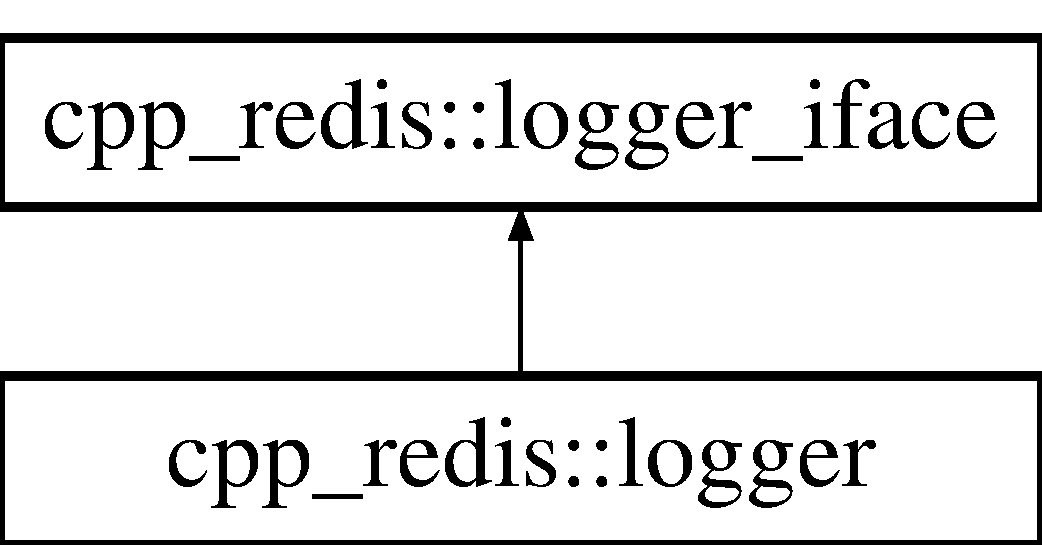
\includegraphics[height=2.000000cm]{classcpp__redis_1_1logger}
\end{center}
\end{figure}
\subsection*{Public Types}
\begin{DoxyCompactItemize}
\item 
enum \mbox{\hyperlink{classcpp__redis_1_1logger_a9493594d547e7abe71b8690be1946c7a}{log\+\_\+level}} \{ {\bfseries error} = 0, 
{\bfseries warn} = 1, 
{\bfseries info} = 2, 
{\bfseries debug} = 3
 \}
\end{DoxyCompactItemize}
\subsection*{Public Member Functions}
\begin{DoxyCompactItemize}
\item 
\mbox{\Hypertarget{classcpp__redis_1_1logger_a36b15a75690a087fca7d304852785512}\label{classcpp__redis_1_1logger_a36b15a75690a087fca7d304852785512}} 
\mbox{\hyperlink{classcpp__redis_1_1logger_a36b15a75690a087fca7d304852785512}{logger}} (\mbox{\hyperlink{classcpp__redis_1_1logger_a9493594d547e7abe71b8690be1946c7a}{log\+\_\+level}} level=log\+\_\+level\+::info)
\begin{DoxyCompactList}\small\item\em ctor \end{DoxyCompactList}\item 
\mbox{\Hypertarget{classcpp__redis_1_1logger_ab5eb02b26c96a6e5cba9a7d30669f625}\label{classcpp__redis_1_1logger_ab5eb02b26c96a6e5cba9a7d30669f625}} 
\mbox{\hyperlink{classcpp__redis_1_1logger_ab5eb02b26c96a6e5cba9a7d30669f625}{$\sim$logger}} (void)=default
\begin{DoxyCompactList}\small\item\em dtor \end{DoxyCompactList}\item 
\mbox{\Hypertarget{classcpp__redis_1_1logger_aec0854d47a13f91e09db25e745a3d722}\label{classcpp__redis_1_1logger_aec0854d47a13f91e09db25e745a3d722}} 
\mbox{\hyperlink{classcpp__redis_1_1logger_aec0854d47a13f91e09db25e745a3d722}{logger}} (const \mbox{\hyperlink{classcpp__redis_1_1logger}{logger}} \&)=default
\begin{DoxyCompactList}\small\item\em copy ctor \end{DoxyCompactList}\item 
\mbox{\Hypertarget{classcpp__redis_1_1logger_a09d012d32f35421a16ec73143adc4415}\label{classcpp__redis_1_1logger_a09d012d32f35421a16ec73143adc4415}} 
\mbox{\hyperlink{classcpp__redis_1_1logger}{logger}} \& \mbox{\hyperlink{classcpp__redis_1_1logger_a09d012d32f35421a16ec73143adc4415}{operator=}} (const \mbox{\hyperlink{classcpp__redis_1_1logger}{logger}} \&)=default
\begin{DoxyCompactList}\small\item\em assignment operator \end{DoxyCompactList}\item 
void \mbox{\hyperlink{classcpp__redis_1_1logger_a36e0908e7b05850b663a4b8b9cdbc299}{debug}} (const std\+::string \&msg, const std\+::string \&file, std\+::size\+\_\+t line)
\item 
void \mbox{\hyperlink{classcpp__redis_1_1logger_a04c741b5110946e76bb23728da6fb2ac}{info}} (const std\+::string \&msg, const std\+::string \&file, std\+::size\+\_\+t line)
\item 
void \mbox{\hyperlink{classcpp__redis_1_1logger_ae9359429428786c7b5605a1109508ae5}{warn}} (const std\+::string \&msg, const std\+::string \&file, std\+::size\+\_\+t line)
\item 
void \mbox{\hyperlink{classcpp__redis_1_1logger_aaf7f2837511f4414a4d7b7b923ebc15e}{error}} (const std\+::string \&msg, const std\+::string \&file, std\+::size\+\_\+t line)
\end{DoxyCompactItemize}


\subsection{Detailed Description}
default logger class provided by the library 

\subsection{Member Enumeration Documentation}
\mbox{\Hypertarget{classcpp__redis_1_1logger_a9493594d547e7abe71b8690be1946c7a}\label{classcpp__redis_1_1logger_a9493594d547e7abe71b8690be1946c7a}} 
\index{cpp\+\_\+redis\+::logger@{cpp\+\_\+redis\+::logger}!log\+\_\+level@{log\+\_\+level}}
\index{log\+\_\+level@{log\+\_\+level}!cpp\+\_\+redis\+::logger@{cpp\+\_\+redis\+::logger}}
\subsubsection{\texorpdfstring{log\+\_\+level}{log\_level}}
{\footnotesize\ttfamily enum \mbox{\hyperlink{classcpp__redis_1_1logger_a9493594d547e7abe71b8690be1946c7a}{cpp\+\_\+redis\+::logger\+::log\+\_\+level}}\hspace{0.3cm}{\ttfamily [strong]}}

log level 

\subsection{Member Function Documentation}
\mbox{\Hypertarget{classcpp__redis_1_1logger_a36e0908e7b05850b663a4b8b9cdbc299}\label{classcpp__redis_1_1logger_a36e0908e7b05850b663a4b8b9cdbc299}} 
\index{cpp\+\_\+redis\+::logger@{cpp\+\_\+redis\+::logger}!debug@{debug}}
\index{debug@{debug}!cpp\+\_\+redis\+::logger@{cpp\+\_\+redis\+::logger}}
\subsubsection{\texorpdfstring{debug()}{debug()}}
{\footnotesize\ttfamily void cpp\+\_\+redis\+::logger\+::debug (\begin{DoxyParamCaption}\item[{const std\+::string \&}]{msg,  }\item[{const std\+::string \&}]{file,  }\item[{std\+::size\+\_\+t}]{line }\end{DoxyParamCaption})\hspace{0.3cm}{\ttfamily [virtual]}}

debug logging


\begin{DoxyParams}{Parameters}
{\em msg} & message to be logged \\
\hline
{\em file} & file from which the message is coming \\
\hline
{\em line} & line in the file of the message \\
\hline
\end{DoxyParams}


Implements \mbox{\hyperlink{classcpp__redis_1_1logger__iface_aaace9e12cbb32d7bdd76c17180a30de7}{cpp\+\_\+redis\+::logger\+\_\+iface}}.

\mbox{\Hypertarget{classcpp__redis_1_1logger_aaf7f2837511f4414a4d7b7b923ebc15e}\label{classcpp__redis_1_1logger_aaf7f2837511f4414a4d7b7b923ebc15e}} 
\index{cpp\+\_\+redis\+::logger@{cpp\+\_\+redis\+::logger}!error@{error}}
\index{error@{error}!cpp\+\_\+redis\+::logger@{cpp\+\_\+redis\+::logger}}
\subsubsection{\texorpdfstring{error()}{error()}}
{\footnotesize\ttfamily void cpp\+\_\+redis\+::logger\+::error (\begin{DoxyParamCaption}\item[{const std\+::string \&}]{msg,  }\item[{const std\+::string \&}]{file,  }\item[{std\+::size\+\_\+t}]{line }\end{DoxyParamCaption})\hspace{0.3cm}{\ttfamily [virtual]}}

error logging


\begin{DoxyParams}{Parameters}
{\em msg} & message to be logged \\
\hline
{\em file} & file from which the message is coming \\
\hline
{\em line} & line in the file of the message \\
\hline
\end{DoxyParams}


Implements \mbox{\hyperlink{classcpp__redis_1_1logger__iface_ac8353031252c80e69e35f5f131870ddf}{cpp\+\_\+redis\+::logger\+\_\+iface}}.

\mbox{\Hypertarget{classcpp__redis_1_1logger_a04c741b5110946e76bb23728da6fb2ac}\label{classcpp__redis_1_1logger_a04c741b5110946e76bb23728da6fb2ac}} 
\index{cpp\+\_\+redis\+::logger@{cpp\+\_\+redis\+::logger}!info@{info}}
\index{info@{info}!cpp\+\_\+redis\+::logger@{cpp\+\_\+redis\+::logger}}
\subsubsection{\texorpdfstring{info()}{info()}}
{\footnotesize\ttfamily void cpp\+\_\+redis\+::logger\+::info (\begin{DoxyParamCaption}\item[{const std\+::string \&}]{msg,  }\item[{const std\+::string \&}]{file,  }\item[{std\+::size\+\_\+t}]{line }\end{DoxyParamCaption})\hspace{0.3cm}{\ttfamily [virtual]}}

info logging


\begin{DoxyParams}{Parameters}
{\em msg} & message to be logged \\
\hline
{\em file} & file from which the message is coming \\
\hline
{\em line} & line in the file of the message \\
\hline
\end{DoxyParams}


Implements \mbox{\hyperlink{classcpp__redis_1_1logger__iface_a02e62f55d7da56efa3b47f2b05931b3b}{cpp\+\_\+redis\+::logger\+\_\+iface}}.

\mbox{\Hypertarget{classcpp__redis_1_1logger_ae9359429428786c7b5605a1109508ae5}\label{classcpp__redis_1_1logger_ae9359429428786c7b5605a1109508ae5}} 
\index{cpp\+\_\+redis\+::logger@{cpp\+\_\+redis\+::logger}!warn@{warn}}
\index{warn@{warn}!cpp\+\_\+redis\+::logger@{cpp\+\_\+redis\+::logger}}
\subsubsection{\texorpdfstring{warn()}{warn()}}
{\footnotesize\ttfamily void cpp\+\_\+redis\+::logger\+::warn (\begin{DoxyParamCaption}\item[{const std\+::string \&}]{msg,  }\item[{const std\+::string \&}]{file,  }\item[{std\+::size\+\_\+t}]{line }\end{DoxyParamCaption})\hspace{0.3cm}{\ttfamily [virtual]}}

warn logging


\begin{DoxyParams}{Parameters}
{\em msg} & message to be logged \\
\hline
{\em file} & file from which the message is coming \\
\hline
{\em line} & line in the file of the message \\
\hline
\end{DoxyParams}


Implements \mbox{\hyperlink{classcpp__redis_1_1logger__iface_a0ea8e43a4f2118e77af56cd1cdb21cba}{cpp\+\_\+redis\+::logger\+\_\+iface}}.



The documentation for this class was generated from the following file\+:\begin{DoxyCompactItemize}
\item 
includes/cpp\+\_\+redis/misc/logger.\+hpp\end{DoxyCompactItemize}

\hypertarget{classcpp__redis_1_1logger__iface}{}\section{cpp\+\_\+redis\+:\+:logger\+\_\+iface Class Reference}
\label{classcpp__redis_1_1logger__iface}\index{cpp\+\_\+redis\+::logger\+\_\+iface@{cpp\+\_\+redis\+::logger\+\_\+iface}}


{\ttfamily \#include $<$logger.\+hpp$>$}

Inheritance diagram for cpp\+\_\+redis\+:\+:logger\+\_\+iface\+:\begin{figure}[H]
\begin{center}
\leavevmode
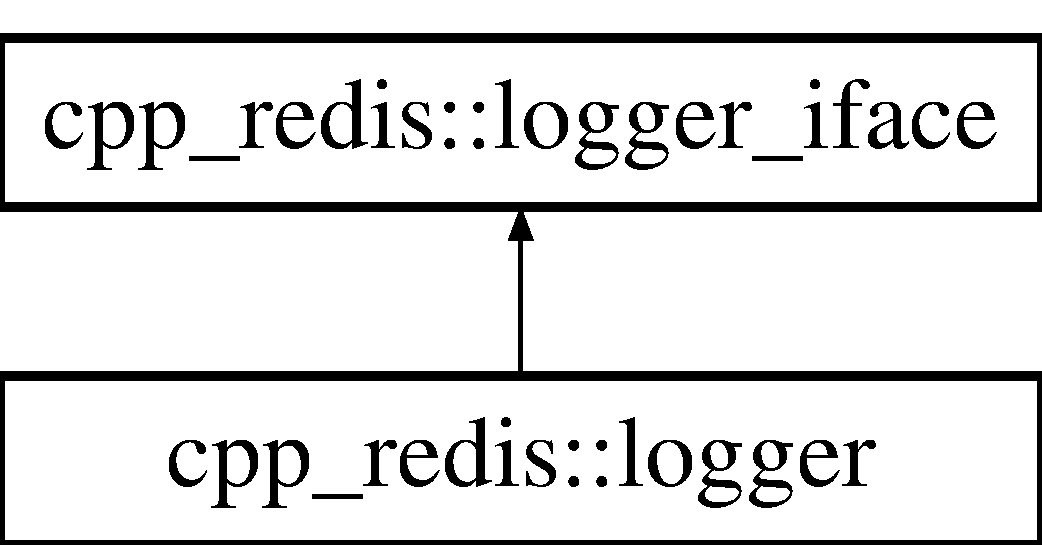
\includegraphics[height=2.000000cm]{classcpp__redis_1_1logger__iface}
\end{center}
\end{figure}
\subsection*{Public Member Functions}
\begin{DoxyCompactItemize}
\item 
\mbox{\Hypertarget{classcpp__redis_1_1logger__iface_a902e41bf0777b960b6575e7ac986147b}\label{classcpp__redis_1_1logger__iface_a902e41bf0777b960b6575e7ac986147b}} 
\mbox{\hyperlink{classcpp__redis_1_1logger__iface_a902e41bf0777b960b6575e7ac986147b}{logger\+\_\+iface}} (void)=default
\begin{DoxyCompactList}\small\item\em ctor \end{DoxyCompactList}\item 
\mbox{\Hypertarget{classcpp__redis_1_1logger__iface_ac7ed1b828afd2e6589fcdda167d34aa5}\label{classcpp__redis_1_1logger__iface_ac7ed1b828afd2e6589fcdda167d34aa5}} 
virtual \mbox{\hyperlink{classcpp__redis_1_1logger__iface_ac7ed1b828afd2e6589fcdda167d34aa5}{$\sim$logger\+\_\+iface}} (void)=default
\begin{DoxyCompactList}\small\item\em dtor \end{DoxyCompactList}\item 
\mbox{\Hypertarget{classcpp__redis_1_1logger__iface_a7f1cb271b18e40f2dde7e45028e69a84}\label{classcpp__redis_1_1logger__iface_a7f1cb271b18e40f2dde7e45028e69a84}} 
\mbox{\hyperlink{classcpp__redis_1_1logger__iface_a7f1cb271b18e40f2dde7e45028e69a84}{logger\+\_\+iface}} (const \mbox{\hyperlink{classcpp__redis_1_1logger__iface}{logger\+\_\+iface}} \&)=default
\begin{DoxyCompactList}\small\item\em copy ctor \end{DoxyCompactList}\item 
\mbox{\Hypertarget{classcpp__redis_1_1logger__iface_a04324701cb81ba6a23f73025b0b3eee0}\label{classcpp__redis_1_1logger__iface_a04324701cb81ba6a23f73025b0b3eee0}} 
\mbox{\hyperlink{classcpp__redis_1_1logger__iface}{logger\+\_\+iface}} \& \mbox{\hyperlink{classcpp__redis_1_1logger__iface_a04324701cb81ba6a23f73025b0b3eee0}{operator=}} (const \mbox{\hyperlink{classcpp__redis_1_1logger__iface}{logger\+\_\+iface}} \&)=default
\begin{DoxyCompactList}\small\item\em assignment operator \end{DoxyCompactList}\item 
virtual void \mbox{\hyperlink{classcpp__redis_1_1logger__iface_aaace9e12cbb32d7bdd76c17180a30de7}{debug}} (const std\+::string \&msg, const std\+::string \&file, std\+::size\+\_\+t line)=0
\item 
virtual void \mbox{\hyperlink{classcpp__redis_1_1logger__iface_a02e62f55d7da56efa3b47f2b05931b3b}{info}} (const std\+::string \&msg, const std\+::string \&file, std\+::size\+\_\+t line)=0
\item 
virtual void \mbox{\hyperlink{classcpp__redis_1_1logger__iface_a0ea8e43a4f2118e77af56cd1cdb21cba}{warn}} (const std\+::string \&msg, const std\+::string \&file, std\+::size\+\_\+t line)=0
\item 
virtual void \mbox{\hyperlink{classcpp__redis_1_1logger__iface_ac8353031252c80e69e35f5f131870ddf}{error}} (const std\+::string \&msg, const std\+::string \&file, std\+::size\+\_\+t line)=0
\end{DoxyCompactItemize}


\subsection{Detailed Description}
\mbox{\hyperlink{classcpp__redis_1_1logger__iface}{logger\+\_\+iface}} should be inherited by any class intended to be used for logging 

\subsection{Member Function Documentation}
\mbox{\Hypertarget{classcpp__redis_1_1logger__iface_aaace9e12cbb32d7bdd76c17180a30de7}\label{classcpp__redis_1_1logger__iface_aaace9e12cbb32d7bdd76c17180a30de7}} 
\index{cpp\+\_\+redis\+::logger\+\_\+iface@{cpp\+\_\+redis\+::logger\+\_\+iface}!debug@{debug}}
\index{debug@{debug}!cpp\+\_\+redis\+::logger\+\_\+iface@{cpp\+\_\+redis\+::logger\+\_\+iface}}
\subsubsection{\texorpdfstring{debug()}{debug()}}
{\footnotesize\ttfamily virtual void cpp\+\_\+redis\+::logger\+\_\+iface\+::debug (\begin{DoxyParamCaption}\item[{const std\+::string \&}]{msg,  }\item[{const std\+::string \&}]{file,  }\item[{std\+::size\+\_\+t}]{line }\end{DoxyParamCaption})\hspace{0.3cm}{\ttfamily [pure virtual]}}

debug logging


\begin{DoxyParams}{Parameters}
{\em msg} & message to be logged \\
\hline
{\em file} & file from which the message is coming \\
\hline
{\em line} & line in the file of the message \\
\hline
\end{DoxyParams}


Implemented in \mbox{\hyperlink{classcpp__redis_1_1logger_a36e0908e7b05850b663a4b8b9cdbc299}{cpp\+\_\+redis\+::logger}}.

\mbox{\Hypertarget{classcpp__redis_1_1logger__iface_ac8353031252c80e69e35f5f131870ddf}\label{classcpp__redis_1_1logger__iface_ac8353031252c80e69e35f5f131870ddf}} 
\index{cpp\+\_\+redis\+::logger\+\_\+iface@{cpp\+\_\+redis\+::logger\+\_\+iface}!error@{error}}
\index{error@{error}!cpp\+\_\+redis\+::logger\+\_\+iface@{cpp\+\_\+redis\+::logger\+\_\+iface}}
\subsubsection{\texorpdfstring{error()}{error()}}
{\footnotesize\ttfamily virtual void cpp\+\_\+redis\+::logger\+\_\+iface\+::error (\begin{DoxyParamCaption}\item[{const std\+::string \&}]{msg,  }\item[{const std\+::string \&}]{file,  }\item[{std\+::size\+\_\+t}]{line }\end{DoxyParamCaption})\hspace{0.3cm}{\ttfamily [pure virtual]}}

error logging


\begin{DoxyParams}{Parameters}
{\em msg} & message to be logged \\
\hline
{\em file} & file from which the message is coming \\
\hline
{\em line} & line in the file of the message \\
\hline
\end{DoxyParams}


Implemented in \mbox{\hyperlink{classcpp__redis_1_1logger_aaf7f2837511f4414a4d7b7b923ebc15e}{cpp\+\_\+redis\+::logger}}.

\mbox{\Hypertarget{classcpp__redis_1_1logger__iface_a02e62f55d7da56efa3b47f2b05931b3b}\label{classcpp__redis_1_1logger__iface_a02e62f55d7da56efa3b47f2b05931b3b}} 
\index{cpp\+\_\+redis\+::logger\+\_\+iface@{cpp\+\_\+redis\+::logger\+\_\+iface}!info@{info}}
\index{info@{info}!cpp\+\_\+redis\+::logger\+\_\+iface@{cpp\+\_\+redis\+::logger\+\_\+iface}}
\subsubsection{\texorpdfstring{info()}{info()}}
{\footnotesize\ttfamily virtual void cpp\+\_\+redis\+::logger\+\_\+iface\+::info (\begin{DoxyParamCaption}\item[{const std\+::string \&}]{msg,  }\item[{const std\+::string \&}]{file,  }\item[{std\+::size\+\_\+t}]{line }\end{DoxyParamCaption})\hspace{0.3cm}{\ttfamily [pure virtual]}}

info logging


\begin{DoxyParams}{Parameters}
{\em msg} & message to be logged \\
\hline
{\em file} & file from which the message is coming \\
\hline
{\em line} & line in the file of the message \\
\hline
\end{DoxyParams}


Implemented in \mbox{\hyperlink{classcpp__redis_1_1logger_a04c741b5110946e76bb23728da6fb2ac}{cpp\+\_\+redis\+::logger}}.

\mbox{\Hypertarget{classcpp__redis_1_1logger__iface_a0ea8e43a4f2118e77af56cd1cdb21cba}\label{classcpp__redis_1_1logger__iface_a0ea8e43a4f2118e77af56cd1cdb21cba}} 
\index{cpp\+\_\+redis\+::logger\+\_\+iface@{cpp\+\_\+redis\+::logger\+\_\+iface}!warn@{warn}}
\index{warn@{warn}!cpp\+\_\+redis\+::logger\+\_\+iface@{cpp\+\_\+redis\+::logger\+\_\+iface}}
\subsubsection{\texorpdfstring{warn()}{warn()}}
{\footnotesize\ttfamily virtual void cpp\+\_\+redis\+::logger\+\_\+iface\+::warn (\begin{DoxyParamCaption}\item[{const std\+::string \&}]{msg,  }\item[{const std\+::string \&}]{file,  }\item[{std\+::size\+\_\+t}]{line }\end{DoxyParamCaption})\hspace{0.3cm}{\ttfamily [pure virtual]}}

warn logging


\begin{DoxyParams}{Parameters}
{\em msg} & message to be logged \\
\hline
{\em file} & file from which the message is coming \\
\hline
{\em line} & line in the file of the message \\
\hline
\end{DoxyParams}


Implemented in \mbox{\hyperlink{classcpp__redis_1_1logger_ae9359429428786c7b5605a1109508ae5}{cpp\+\_\+redis\+::logger}}.



The documentation for this class was generated from the following file\+:\begin{DoxyCompactItemize}
\item 
includes/cpp\+\_\+redis/misc/logger.\+hpp\end{DoxyCompactItemize}

\hypertarget{structcpp__redis_1_1network_1_1tcp__client__iface_1_1read__request}{}\section{cpp\+\_\+redis\+:\+:network\+:\+:tcp\+\_\+client\+\_\+iface\+:\+:read\+\_\+request Struct Reference}
\label{structcpp__redis_1_1network_1_1tcp__client__iface_1_1read__request}\index{cpp\+\_\+redis\+::network\+::tcp\+\_\+client\+\_\+iface\+::read\+\_\+request@{cpp\+\_\+redis\+::network\+::tcp\+\_\+client\+\_\+iface\+::read\+\_\+request}}


{\ttfamily \#include $<$tcp\+\_\+client\+\_\+iface.\+hpp$>$}

\subsection*{Public Attributes}
\begin{DoxyCompactItemize}
\item 
std\+::size\+\_\+t \mbox{\hyperlink{structcpp__redis_1_1network_1_1tcp__client__iface_1_1read__request_a5ff8258391c9b3c8d2ce1a5c5a0304be}{size}}
\item 
\mbox{\hyperlink{classcpp__redis_1_1network_1_1tcp__client__iface_ae8bf79e8e1f1d7e359ed1c7cdc4026fc}{async\+\_\+read\+\_\+callback\+\_\+t}} \mbox{\hyperlink{structcpp__redis_1_1network_1_1tcp__client__iface_1_1read__request_a0584269b3a021d588e38948c12fa5292}{async\+\_\+read\+\_\+callback}}
\end{DoxyCompactItemize}


\subsection{Detailed Description}
structure to store read requests information 

\subsection{Member Data Documentation}
\mbox{\Hypertarget{structcpp__redis_1_1network_1_1tcp__client__iface_1_1read__request_a0584269b3a021d588e38948c12fa5292}\label{structcpp__redis_1_1network_1_1tcp__client__iface_1_1read__request_a0584269b3a021d588e38948c12fa5292}} 
\index{cpp\+\_\+redis\+::network\+::tcp\+\_\+client\+\_\+iface\+::read\+\_\+request@{cpp\+\_\+redis\+::network\+::tcp\+\_\+client\+\_\+iface\+::read\+\_\+request}!async\+\_\+read\+\_\+callback@{async\+\_\+read\+\_\+callback}}
\index{async\+\_\+read\+\_\+callback@{async\+\_\+read\+\_\+callback}!cpp\+\_\+redis\+::network\+::tcp\+\_\+client\+\_\+iface\+::read\+\_\+request@{cpp\+\_\+redis\+::network\+::tcp\+\_\+client\+\_\+iface\+::read\+\_\+request}}
\subsubsection{\texorpdfstring{async\+\_\+read\+\_\+callback}{async\_read\_callback}}
{\footnotesize\ttfamily \mbox{\hyperlink{classcpp__redis_1_1network_1_1tcp__client__iface_ae8bf79e8e1f1d7e359ed1c7cdc4026fc}{async\+\_\+read\+\_\+callback\+\_\+t}} cpp\+\_\+redis\+::network\+::tcp\+\_\+client\+\_\+iface\+::read\+\_\+request\+::async\+\_\+read\+\_\+callback}

callback to be called on operation completion \mbox{\Hypertarget{structcpp__redis_1_1network_1_1tcp__client__iface_1_1read__request_a5ff8258391c9b3c8d2ce1a5c5a0304be}\label{structcpp__redis_1_1network_1_1tcp__client__iface_1_1read__request_a5ff8258391c9b3c8d2ce1a5c5a0304be}} 
\index{cpp\+\_\+redis\+::network\+::tcp\+\_\+client\+\_\+iface\+::read\+\_\+request@{cpp\+\_\+redis\+::network\+::tcp\+\_\+client\+\_\+iface\+::read\+\_\+request}!size@{size}}
\index{size@{size}!cpp\+\_\+redis\+::network\+::tcp\+\_\+client\+\_\+iface\+::read\+\_\+request@{cpp\+\_\+redis\+::network\+::tcp\+\_\+client\+\_\+iface\+::read\+\_\+request}}
\subsubsection{\texorpdfstring{size}{size}}
{\footnotesize\ttfamily std\+::size\+\_\+t cpp\+\_\+redis\+::network\+::tcp\+\_\+client\+\_\+iface\+::read\+\_\+request\+::size}

number of bytes to read 

The documentation for this struct was generated from the following file\+:\begin{DoxyCompactItemize}
\item 
includes/cpp\+\_\+redis/network/tcp\+\_\+client\+\_\+iface.\+hpp\end{DoxyCompactItemize}

\hypertarget{structcpp__redis_1_1network_1_1tcp__client__iface_1_1read__result}{}\section{cpp\+\_\+redis\+:\+:network\+:\+:tcp\+\_\+client\+\_\+iface\+:\+:read\+\_\+result Struct Reference}
\label{structcpp__redis_1_1network_1_1tcp__client__iface_1_1read__result}\index{cpp\+\_\+redis\+::network\+::tcp\+\_\+client\+\_\+iface\+::read\+\_\+result@{cpp\+\_\+redis\+::network\+::tcp\+\_\+client\+\_\+iface\+::read\+\_\+result}}


{\ttfamily \#include $<$tcp\+\_\+client\+\_\+iface.\+hpp$>$}

\subsection*{Public Attributes}
\begin{DoxyCompactItemize}
\item 
bool \hyperlink{structcpp__redis_1_1network_1_1tcp__client__iface_1_1read__result_ab9a3a54474c382a00323ed02f4239faa}{success}
\item 
std\+::vector$<$ char $>$ \hyperlink{structcpp__redis_1_1network_1_1tcp__client__iface_1_1read__result_af8275097ebe558e7ce0f2aa29131cb05}{buffer}
\end{DoxyCompactItemize}


\subsection{Detailed Description}
structure to store read requests result 

\subsection{Member Data Documentation}
\mbox{\Hypertarget{structcpp__redis_1_1network_1_1tcp__client__iface_1_1read__result_af8275097ebe558e7ce0f2aa29131cb05}\label{structcpp__redis_1_1network_1_1tcp__client__iface_1_1read__result_af8275097ebe558e7ce0f2aa29131cb05}} 
\index{cpp\+\_\+redis\+::network\+::tcp\+\_\+client\+\_\+iface\+::read\+\_\+result@{cpp\+\_\+redis\+::network\+::tcp\+\_\+client\+\_\+iface\+::read\+\_\+result}!buffer@{buffer}}
\index{buffer@{buffer}!cpp\+\_\+redis\+::network\+::tcp\+\_\+client\+\_\+iface\+::read\+\_\+result@{cpp\+\_\+redis\+::network\+::tcp\+\_\+client\+\_\+iface\+::read\+\_\+result}}
\subsubsection{\texorpdfstring{buffer}{buffer}}
{\footnotesize\ttfamily std\+::vector$<$char$>$ cpp\+\_\+redis\+::network\+::tcp\+\_\+client\+\_\+iface\+::read\+\_\+result\+::buffer}

read bytes \mbox{\Hypertarget{structcpp__redis_1_1network_1_1tcp__client__iface_1_1read__result_ab9a3a54474c382a00323ed02f4239faa}\label{structcpp__redis_1_1network_1_1tcp__client__iface_1_1read__result_ab9a3a54474c382a00323ed02f4239faa}} 
\index{cpp\+\_\+redis\+::network\+::tcp\+\_\+client\+\_\+iface\+::read\+\_\+result@{cpp\+\_\+redis\+::network\+::tcp\+\_\+client\+\_\+iface\+::read\+\_\+result}!success@{success}}
\index{success@{success}!cpp\+\_\+redis\+::network\+::tcp\+\_\+client\+\_\+iface\+::read\+\_\+result@{cpp\+\_\+redis\+::network\+::tcp\+\_\+client\+\_\+iface\+::read\+\_\+result}}
\subsubsection{\texorpdfstring{success}{success}}
{\footnotesize\ttfamily bool cpp\+\_\+redis\+::network\+::tcp\+\_\+client\+\_\+iface\+::read\+\_\+result\+::success}

whether the operation succeeded or not 

The documentation for this struct was generated from the following file\+:\begin{DoxyCompactItemize}
\item 
includes/cpp\+\_\+redis/network/tcp\+\_\+client\+\_\+iface.\+hpp\end{DoxyCompactItemize}

\hypertarget{classcpp__redis_1_1network_1_1redis__connection}{}\section{cpp\+\_\+redis\+:\+:network\+:\+:redis\+\_\+connection Class Reference}
\label{classcpp__redis_1_1network_1_1redis__connection}\index{cpp\+\_\+redis\+::network\+::redis\+\_\+connection@{cpp\+\_\+redis\+::network\+::redis\+\_\+connection}}


{\ttfamily \#include $<$redis\+\_\+connection.\+hpp$>$}

\subsection*{Public Types}
\begin{DoxyCompactItemize}
\item 
typedef std\+::function$<$ void(\mbox{\hyperlink{classcpp__redis_1_1network_1_1redis__connection}{redis\+\_\+connection}} \&)$>$ \mbox{\hyperlink{classcpp__redis_1_1network_1_1redis__connection_aba1a229a3d36a5540a80776ed0cf9a44}{disconnection\+\_\+handler\+\_\+t}}
\item 
typedef std\+::function$<$ void(\mbox{\hyperlink{classcpp__redis_1_1network_1_1redis__connection}{redis\+\_\+connection}} \&, \mbox{\hyperlink{classcpp__redis_1_1reply}{reply}} \&)$>$ \mbox{\hyperlink{classcpp__redis_1_1network_1_1redis__connection_a40f4b55a3103b7436e34211893377245}{reply\+\_\+callback\+\_\+t}}
\end{DoxyCompactItemize}
\subsection*{Public Member Functions}
\begin{DoxyCompactItemize}
\item 
\mbox{\Hypertarget{classcpp__redis_1_1network_1_1redis__connection_aee0302e4ff9c9b5b2e7f467d869d45f7}\label{classcpp__redis_1_1network_1_1redis__connection_aee0302e4ff9c9b5b2e7f467d869d45f7}} 
\mbox{\hyperlink{classcpp__redis_1_1network_1_1redis__connection_aee0302e4ff9c9b5b2e7f467d869d45f7}{redis\+\_\+connection}} (void)
\begin{DoxyCompactList}\small\item\em ctor \end{DoxyCompactList}\item 
\mbox{\hyperlink{classcpp__redis_1_1network_1_1redis__connection_a6880cfb2e1b037fcdaa5f0a6d515b375}{redis\+\_\+connection}} (const std\+::shared\+\_\+ptr$<$ \mbox{\hyperlink{classcpp__redis_1_1network_1_1tcp__client__iface}{tcp\+\_\+client\+\_\+iface}} $>$ \&\mbox{\hyperlink{classcpp__redis_1_1network_1_1tcp__client}{tcp\+\_\+client}})
\item 
\mbox{\Hypertarget{classcpp__redis_1_1network_1_1redis__connection_a9d392191ce262eddd5570b57e07aa051}\label{classcpp__redis_1_1network_1_1redis__connection_a9d392191ce262eddd5570b57e07aa051}} 
\mbox{\hyperlink{classcpp__redis_1_1network_1_1redis__connection_a9d392191ce262eddd5570b57e07aa051}{$\sim$redis\+\_\+connection}} (void)
\begin{DoxyCompactList}\small\item\em dtor \end{DoxyCompactList}\item 
\mbox{\Hypertarget{classcpp__redis_1_1network_1_1redis__connection_a2bdd38bbfd5d97aeca8e433465c4d621}\label{classcpp__redis_1_1network_1_1redis__connection_a2bdd38bbfd5d97aeca8e433465c4d621}} 
\mbox{\hyperlink{classcpp__redis_1_1network_1_1redis__connection_a2bdd38bbfd5d97aeca8e433465c4d621}{redis\+\_\+connection}} (const \mbox{\hyperlink{classcpp__redis_1_1network_1_1redis__connection}{redis\+\_\+connection}} \&)=delete
\begin{DoxyCompactList}\small\item\em copy ctor \end{DoxyCompactList}\item 
\mbox{\Hypertarget{classcpp__redis_1_1network_1_1redis__connection_a54a4c28ad1b9e9f3bac2854fddf4e30d}\label{classcpp__redis_1_1network_1_1redis__connection_a54a4c28ad1b9e9f3bac2854fddf4e30d}} 
\mbox{\hyperlink{classcpp__redis_1_1network_1_1redis__connection}{redis\+\_\+connection}} \& \mbox{\hyperlink{classcpp__redis_1_1network_1_1redis__connection_a54a4c28ad1b9e9f3bac2854fddf4e30d}{operator=}} (const \mbox{\hyperlink{classcpp__redis_1_1network_1_1redis__connection}{redis\+\_\+connection}} \&)=delete
\begin{DoxyCompactList}\small\item\em assignment operator \end{DoxyCompactList}\item 
void \mbox{\hyperlink{classcpp__redis_1_1network_1_1redis__connection_af105573e46eadbc34a9f5907832df19f}{connect}} (const std\+::string \&host=\char`\"{}127.\+0.\+0.\+1\char`\"{}, std\+::size\+\_\+t port=6379, const \mbox{\hyperlink{classcpp__redis_1_1network_1_1redis__connection_aba1a229a3d36a5540a80776ed0cf9a44}{disconnection\+\_\+handler\+\_\+t}} \&disconnection\+\_\+handler=nullptr, const \mbox{\hyperlink{classcpp__redis_1_1network_1_1redis__connection_a40f4b55a3103b7436e34211893377245}{reply\+\_\+callback\+\_\+t}} \&reply\+\_\+callback=nullptr, std\+::uint32\+\_\+t timeout\+\_\+msecs=0)
\item 
void \mbox{\hyperlink{classcpp__redis_1_1network_1_1redis__connection_a614a01ce8abd69b44f3d072423d2e696}{disconnect}} (bool wait\+\_\+for\+\_\+removal=false)
\item 
bool \mbox{\hyperlink{classcpp__redis_1_1network_1_1redis__connection_ad3d96826e2e67fb3fed23280237d4d9c}{is\+\_\+connected}} (void) const
\item 
\mbox{\hyperlink{classcpp__redis_1_1network_1_1redis__connection}{redis\+\_\+connection}} \& \mbox{\hyperlink{classcpp__redis_1_1network_1_1redis__connection_a98c163ce431e85e46e139211564b7b3f}{send}} (const std\+::vector$<$ std\+::string $>$ \&redis\+\_\+cmd)
\item 
\mbox{\hyperlink{classcpp__redis_1_1network_1_1redis__connection}{redis\+\_\+connection}} \& \mbox{\hyperlink{classcpp__redis_1_1network_1_1redis__connection_a8e6980d40139877c16e995051b780d60}{commit}} (void)
\end{DoxyCompactItemize}


\subsection{Detailed Description}
tcp connection wrapper handling redis protocol 

\subsection{Member Typedef Documentation}
\mbox{\Hypertarget{classcpp__redis_1_1network_1_1redis__connection_aba1a229a3d36a5540a80776ed0cf9a44}\label{classcpp__redis_1_1network_1_1redis__connection_aba1a229a3d36a5540a80776ed0cf9a44}} 
\index{cpp\+\_\+redis\+::network\+::redis\+\_\+connection@{cpp\+\_\+redis\+::network\+::redis\+\_\+connection}!disconnection\+\_\+handler\+\_\+t@{disconnection\+\_\+handler\+\_\+t}}
\index{disconnection\+\_\+handler\+\_\+t@{disconnection\+\_\+handler\+\_\+t}!cpp\+\_\+redis\+::network\+::redis\+\_\+connection@{cpp\+\_\+redis\+::network\+::redis\+\_\+connection}}
\subsubsection{\texorpdfstring{disconnection\+\_\+handler\+\_\+t}{disconnection\_handler\_t}}
{\footnotesize\ttfamily typedef std\+::function$<$void(\mbox{\hyperlink{classcpp__redis_1_1network_1_1redis__connection}{redis\+\_\+connection}}\&)$>$ \mbox{\hyperlink{classcpp__redis_1_1network_1_1redis__connection_aba1a229a3d36a5540a80776ed0cf9a44}{cpp\+\_\+redis\+::network\+::redis\+\_\+connection\+::disconnection\+\_\+handler\+\_\+t}}}

disconnection handler takes as parameter the instance of the \mbox{\hyperlink{classcpp__redis_1_1network_1_1redis__connection}{redis\+\_\+connection}} \mbox{\Hypertarget{classcpp__redis_1_1network_1_1redis__connection_a40f4b55a3103b7436e34211893377245}\label{classcpp__redis_1_1network_1_1redis__connection_a40f4b55a3103b7436e34211893377245}} 
\index{cpp\+\_\+redis\+::network\+::redis\+\_\+connection@{cpp\+\_\+redis\+::network\+::redis\+\_\+connection}!reply\+\_\+callback\+\_\+t@{reply\+\_\+callback\+\_\+t}}
\index{reply\+\_\+callback\+\_\+t@{reply\+\_\+callback\+\_\+t}!cpp\+\_\+redis\+::network\+::redis\+\_\+connection@{cpp\+\_\+redis\+::network\+::redis\+\_\+connection}}
\subsubsection{\texorpdfstring{reply\+\_\+callback\+\_\+t}{reply\_callback\_t}}
{\footnotesize\ttfamily typedef std\+::function$<$void(\mbox{\hyperlink{classcpp__redis_1_1network_1_1redis__connection}{redis\+\_\+connection}}\&, \mbox{\hyperlink{classcpp__redis_1_1reply}{reply}}\&)$>$ \mbox{\hyperlink{classcpp__redis_1_1network_1_1redis__connection_a40f4b55a3103b7436e34211893377245}{cpp\+\_\+redis\+::network\+::redis\+\_\+connection\+::reply\+\_\+callback\+\_\+t}}}

reply handler takes as parameter the instance of the \mbox{\hyperlink{classcpp__redis_1_1network_1_1redis__connection}{redis\+\_\+connection}} and the built reply 

\subsection{Constructor \& Destructor Documentation}
\mbox{\Hypertarget{classcpp__redis_1_1network_1_1redis__connection_a6880cfb2e1b037fcdaa5f0a6d515b375}\label{classcpp__redis_1_1network_1_1redis__connection_a6880cfb2e1b037fcdaa5f0a6d515b375}} 
\index{cpp\+\_\+redis\+::network\+::redis\+\_\+connection@{cpp\+\_\+redis\+::network\+::redis\+\_\+connection}!redis\+\_\+connection@{redis\+\_\+connection}}
\index{redis\+\_\+connection@{redis\+\_\+connection}!cpp\+\_\+redis\+::network\+::redis\+\_\+connection@{cpp\+\_\+redis\+::network\+::redis\+\_\+connection}}
\subsubsection{\texorpdfstring{redis\+\_\+connection()}{redis\_connection()}}
{\footnotesize\ttfamily cpp\+\_\+redis\+::network\+::redis\+\_\+connection\+::redis\+\_\+connection (\begin{DoxyParamCaption}\item[{const std\+::shared\+\_\+ptr$<$ \mbox{\hyperlink{classcpp__redis_1_1network_1_1tcp__client__iface}{tcp\+\_\+client\+\_\+iface}} $>$ \&}]{tcp\+\_\+client }\end{DoxyParamCaption})\hspace{0.3cm}{\ttfamily [explicit]}}

ctor allowing to specify custom tcp client (default ctor uses the default tacopie tcp client)


\begin{DoxyParams}{Parameters}
{\em \mbox{\hyperlink{classcpp__redis_1_1network_1_1tcp__client}{tcp\+\_\+client}}} & tcp client to be used for network communications \\
\hline
\end{DoxyParams}


\subsection{Member Function Documentation}
\mbox{\Hypertarget{classcpp__redis_1_1network_1_1redis__connection_a8e6980d40139877c16e995051b780d60}\label{classcpp__redis_1_1network_1_1redis__connection_a8e6980d40139877c16e995051b780d60}} 
\index{cpp\+\_\+redis\+::network\+::redis\+\_\+connection@{cpp\+\_\+redis\+::network\+::redis\+\_\+connection}!commit@{commit}}
\index{commit@{commit}!cpp\+\_\+redis\+::network\+::redis\+\_\+connection@{cpp\+\_\+redis\+::network\+::redis\+\_\+connection}}
\subsubsection{\texorpdfstring{commit()}{commit()}}
{\footnotesize\ttfamily \mbox{\hyperlink{classcpp__redis_1_1network_1_1redis__connection}{redis\+\_\+connection}}\& cpp\+\_\+redis\+::network\+::redis\+\_\+connection\+::commit (\begin{DoxyParamCaption}\item[{void}]{ }\end{DoxyParamCaption})}

commit pipelined transaction that is, send to the network all commands pipelined by calling \mbox{\hyperlink{classcpp__redis_1_1network_1_1redis__connection_a98c163ce431e85e46e139211564b7b3f}{send()}}

\begin{DoxyReturn}{Returns}
current instance 
\end{DoxyReturn}
\mbox{\Hypertarget{classcpp__redis_1_1network_1_1redis__connection_af105573e46eadbc34a9f5907832df19f}\label{classcpp__redis_1_1network_1_1redis__connection_af105573e46eadbc34a9f5907832df19f}} 
\index{cpp\+\_\+redis\+::network\+::redis\+\_\+connection@{cpp\+\_\+redis\+::network\+::redis\+\_\+connection}!connect@{connect}}
\index{connect@{connect}!cpp\+\_\+redis\+::network\+::redis\+\_\+connection@{cpp\+\_\+redis\+::network\+::redis\+\_\+connection}}
\subsubsection{\texorpdfstring{connect()}{connect()}}
{\footnotesize\ttfamily void cpp\+\_\+redis\+::network\+::redis\+\_\+connection\+::connect (\begin{DoxyParamCaption}\item[{const std\+::string \&}]{host = {\ttfamily \char`\"{}127.0.0.1\char`\"{}},  }\item[{std\+::size\+\_\+t}]{port = {\ttfamily 6379},  }\item[{const \mbox{\hyperlink{classcpp__redis_1_1network_1_1redis__connection_aba1a229a3d36a5540a80776ed0cf9a44}{disconnection\+\_\+handler\+\_\+t}} \&}]{disconnection\+\_\+handler = {\ttfamily nullptr},  }\item[{const \mbox{\hyperlink{classcpp__redis_1_1network_1_1redis__connection_a40f4b55a3103b7436e34211893377245}{reply\+\_\+callback\+\_\+t}} \&}]{reply\+\_\+callback = {\ttfamily nullptr},  }\item[{std\+::uint32\+\_\+t}]{timeout\+\_\+msecs = {\ttfamily 0} }\end{DoxyParamCaption})}

connect to the given host and port, and set both disconnection and reply callbacks


\begin{DoxyParams}{Parameters}
{\em host} & host to be connected to \\
\hline
{\em port} & port to be connected to \\
\hline
{\em disconnection\+\_\+handler} & handler to be called in case of disconnection \\
\hline
{\em reply\+\_\+callback} & handler to be called once a reply is ready \\
\hline
{\em timeout\+\_\+msecs} & max time to connect (in ms) \\
\hline
\end{DoxyParams}
\mbox{\Hypertarget{classcpp__redis_1_1network_1_1redis__connection_a614a01ce8abd69b44f3d072423d2e696}\label{classcpp__redis_1_1network_1_1redis__connection_a614a01ce8abd69b44f3d072423d2e696}} 
\index{cpp\+\_\+redis\+::network\+::redis\+\_\+connection@{cpp\+\_\+redis\+::network\+::redis\+\_\+connection}!disconnect@{disconnect}}
\index{disconnect@{disconnect}!cpp\+\_\+redis\+::network\+::redis\+\_\+connection@{cpp\+\_\+redis\+::network\+::redis\+\_\+connection}}
\subsubsection{\texorpdfstring{disconnect()}{disconnect()}}
{\footnotesize\ttfamily void cpp\+\_\+redis\+::network\+::redis\+\_\+connection\+::disconnect (\begin{DoxyParamCaption}\item[{bool}]{wait\+\_\+for\+\_\+removal = {\ttfamily false} }\end{DoxyParamCaption})}

disconnect from redis server


\begin{DoxyParams}{Parameters}
{\em wait\+\_\+for\+\_\+removal} & when sets to true, disconnect blocks until the underlying T\+CP client has been effectively removed from the io\+\_\+service and that all the underlying callbacks have completed. \\
\hline
\end{DoxyParams}
\mbox{\Hypertarget{classcpp__redis_1_1network_1_1redis__connection_ad3d96826e2e67fb3fed23280237d4d9c}\label{classcpp__redis_1_1network_1_1redis__connection_ad3d96826e2e67fb3fed23280237d4d9c}} 
\index{cpp\+\_\+redis\+::network\+::redis\+\_\+connection@{cpp\+\_\+redis\+::network\+::redis\+\_\+connection}!is\+\_\+connected@{is\+\_\+connected}}
\index{is\+\_\+connected@{is\+\_\+connected}!cpp\+\_\+redis\+::network\+::redis\+\_\+connection@{cpp\+\_\+redis\+::network\+::redis\+\_\+connection}}
\subsubsection{\texorpdfstring{is\+\_\+connected()}{is\_connected()}}
{\footnotesize\ttfamily bool cpp\+\_\+redis\+::network\+::redis\+\_\+connection\+::is\+\_\+connected (\begin{DoxyParamCaption}\item[{void}]{ }\end{DoxyParamCaption}) const}

\begin{DoxyReturn}{Returns}
whether we are connected to the redis server or not 
\end{DoxyReturn}
\mbox{\Hypertarget{classcpp__redis_1_1network_1_1redis__connection_a98c163ce431e85e46e139211564b7b3f}\label{classcpp__redis_1_1network_1_1redis__connection_a98c163ce431e85e46e139211564b7b3f}} 
\index{cpp\+\_\+redis\+::network\+::redis\+\_\+connection@{cpp\+\_\+redis\+::network\+::redis\+\_\+connection}!send@{send}}
\index{send@{send}!cpp\+\_\+redis\+::network\+::redis\+\_\+connection@{cpp\+\_\+redis\+::network\+::redis\+\_\+connection}}
\subsubsection{\texorpdfstring{send()}{send()}}
{\footnotesize\ttfamily \mbox{\hyperlink{classcpp__redis_1_1network_1_1redis__connection}{redis\+\_\+connection}}\& cpp\+\_\+redis\+::network\+::redis\+\_\+connection\+::send (\begin{DoxyParamCaption}\item[{const std\+::vector$<$ std\+::string $>$ \&}]{redis\+\_\+cmd }\end{DoxyParamCaption})}

send the given command the command is actually pipelined and only buffered, so nothing is sent to the network please call \mbox{\hyperlink{classcpp__redis_1_1network_1_1redis__connection_a8e6980d40139877c16e995051b780d60}{commit()}} to flush the buffer


\begin{DoxyParams}{Parameters}
{\em redis\+\_\+cmd} & command to be sent \\
\hline
\end{DoxyParams}
\begin{DoxyReturn}{Returns}
current instance 
\end{DoxyReturn}


The documentation for this class was generated from the following file\+:\begin{DoxyCompactItemize}
\item 
includes/cpp\+\_\+redis/network/redis\+\_\+connection.\+hpp\end{DoxyCompactItemize}

\hypertarget{classcpp__redis_1_1redis__error}{}\section{cpp\+\_\+redis\+:\+:redis\+\_\+error Class Reference}
\label{classcpp__redis_1_1redis__error}\index{cpp\+\_\+redis\+::redis\+\_\+error@{cpp\+\_\+redis\+::redis\+\_\+error}}


{\ttfamily \#include $<$error.\+hpp$>$}

Inheritance diagram for cpp\+\_\+redis\+:\+:redis\+\_\+error\+:\begin{figure}[H]
\begin{center}
\leavevmode
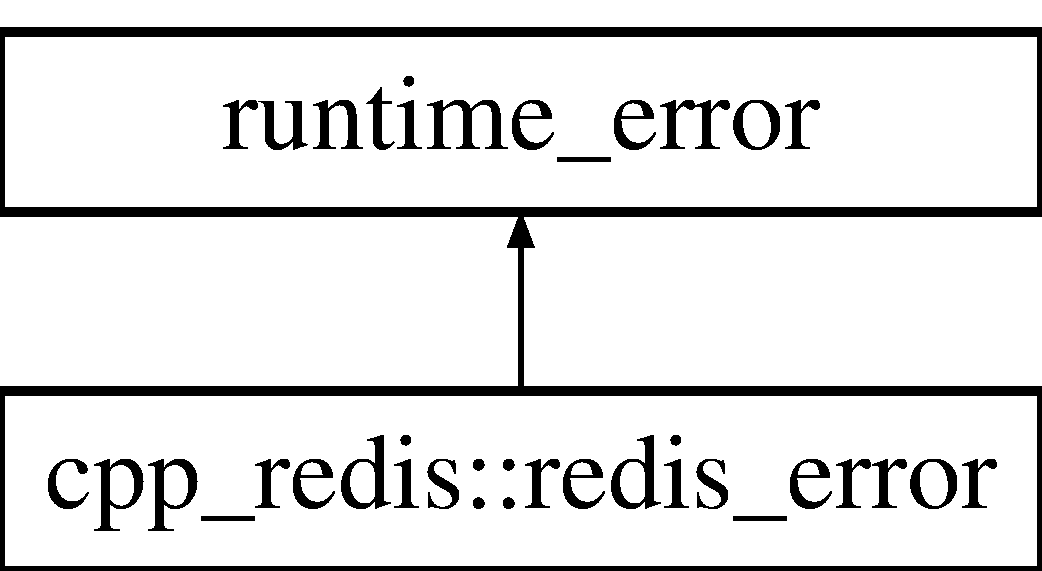
\includegraphics[height=2.000000cm]{classcpp__redis_1_1redis__error}
\end{center}
\end{figure}
\subsection*{Public Member Functions}
\begin{DoxyCompactItemize}
\item 
\hyperlink{classcpp__redis_1_1redis__error_a1445e654b3936c7f5aa1c298bcf24966}{redis\+\_\+error} (const std\+::string \&err)
\begin{DoxyCompactList}\small\item\em ctor (string) \end{DoxyCompactList}\item 
\hyperlink{classcpp__redis_1_1redis__error_a0ced25483119c2318b1a5a69cac1919f}{redis\+\_\+error} (const char $\ast$err)
\begin{DoxyCompactList}\small\item\em ctor(char$\ast$) \end{DoxyCompactList}\end{DoxyCompactItemize}


\subsection{Detailed Description}
specialized runtime\+\_\+error used for \hyperlink{namespacecpp__redis}{cpp\+\_\+redis} error 

\subsection{Constructor \& Destructor Documentation}
\mbox{\Hypertarget{classcpp__redis_1_1redis__error_a1445e654b3936c7f5aa1c298bcf24966}\label{classcpp__redis_1_1redis__error_a1445e654b3936c7f5aa1c298bcf24966}} 
\index{cpp\+\_\+redis\+::redis\+\_\+error@{cpp\+\_\+redis\+::redis\+\_\+error}!redis\+\_\+error@{redis\+\_\+error}}
\index{redis\+\_\+error@{redis\+\_\+error}!cpp\+\_\+redis\+::redis\+\_\+error@{cpp\+\_\+redis\+::redis\+\_\+error}}
\subsubsection{\texorpdfstring{redis\+\_\+error()}{redis\_error()}\hspace{0.1cm}{\footnotesize\ttfamily [1/2]}}
{\footnotesize\ttfamily cpp\+\_\+redis\+::redis\+\_\+error\+::redis\+\_\+error (\begin{DoxyParamCaption}\item[{const std\+::string \&}]{err }\end{DoxyParamCaption})\hspace{0.3cm}{\ttfamily [inline]}, {\ttfamily [explicit]}}



ctor (string) 

\mbox{\Hypertarget{classcpp__redis_1_1redis__error_a0ced25483119c2318b1a5a69cac1919f}\label{classcpp__redis_1_1redis__error_a0ced25483119c2318b1a5a69cac1919f}} 
\index{cpp\+\_\+redis\+::redis\+\_\+error@{cpp\+\_\+redis\+::redis\+\_\+error}!redis\+\_\+error@{redis\+\_\+error}}
\index{redis\+\_\+error@{redis\+\_\+error}!cpp\+\_\+redis\+::redis\+\_\+error@{cpp\+\_\+redis\+::redis\+\_\+error}}
\subsubsection{\texorpdfstring{redis\+\_\+error()}{redis\_error()}\hspace{0.1cm}{\footnotesize\ttfamily [2/2]}}
{\footnotesize\ttfamily cpp\+\_\+redis\+::redis\+\_\+error\+::redis\+\_\+error (\begin{DoxyParamCaption}\item[{const char $\ast$}]{err }\end{DoxyParamCaption})\hspace{0.3cm}{\ttfamily [inline]}, {\ttfamily [explicit]}}



ctor(char$\ast$) 



The documentation for this class was generated from the following file\+:\begin{DoxyCompactItemize}
\item 
includes/cpp\+\_\+redis/misc/\hyperlink{error_8hpp}{error.\+hpp}\end{DoxyCompactItemize}

\hypertarget{classcpp__redis_1_1reply}{}\section{cpp\+\_\+redis\+:\+:reply Class Reference}
\label{classcpp__redis_1_1reply}\index{cpp\+\_\+redis\+::reply@{cpp\+\_\+redis\+::reply}}


{\ttfamily \#include $<$reply.\+hpp$>$}

\subsection*{Public Types}
\begin{DoxyCompactItemize}
\item 
enum \hyperlink{classcpp__redis_1_1reply_acc272b2a52164cac1d110c619a0b25bd}{type} \{ \newline
{\bfseries error} = \+\_\+\+\_\+\+C\+P\+P\+\_\+\+R\+E\+D\+I\+S\+\_\+\+R\+E\+P\+L\+Y\+\_\+\+E\+RR, 
{\bfseries bulk\+\_\+string} = \+\_\+\+\_\+\+C\+P\+P\+\_\+\+R\+E\+D\+I\+S\+\_\+\+R\+E\+P\+L\+Y\+\_\+\+B\+U\+LK, 
{\bfseries simple\+\_\+string} = \+\_\+\+\_\+\+C\+P\+P\+\_\+\+R\+E\+D\+I\+S\+\_\+\+R\+E\+P\+L\+Y\+\_\+\+S\+I\+M\+P\+LE, 
{\bfseries null} = \+\_\+\+\_\+\+C\+P\+P\+\_\+\+R\+E\+D\+I\+S\+\_\+\+R\+E\+P\+L\+Y\+\_\+\+N\+U\+LL, 
\newline
{\bfseries integer} = \+\_\+\+\_\+\+C\+P\+P\+\_\+\+R\+E\+D\+I\+S\+\_\+\+R\+E\+P\+L\+Y\+\_\+\+I\+NT, 
{\bfseries array} = \+\_\+\+\_\+\+C\+P\+P\+\_\+\+R\+E\+D\+I\+S\+\_\+\+R\+E\+P\+L\+Y\+\_\+\+A\+R\+R\+AY
 \}
\item 
enum \hyperlink{classcpp__redis_1_1reply_ac192ba4cb8f2bb6e7cb465edf755328b}{string\+\_\+type} \{ {\bfseries error} = \+\_\+\+\_\+\+C\+P\+P\+\_\+\+R\+E\+D\+I\+S\+\_\+\+R\+E\+P\+L\+Y\+\_\+\+E\+RR, 
{\bfseries bulk\+\_\+string} = \+\_\+\+\_\+\+C\+P\+P\+\_\+\+R\+E\+D\+I\+S\+\_\+\+R\+E\+P\+L\+Y\+\_\+\+B\+U\+LK, 
{\bfseries simple\+\_\+string} = \+\_\+\+\_\+\+C\+P\+P\+\_\+\+R\+E\+D\+I\+S\+\_\+\+R\+E\+P\+L\+Y\+\_\+\+S\+I\+M\+P\+LE
 \}
\end{DoxyCompactItemize}
\subsection*{Public Member Functions}
\begin{DoxyCompactItemize}
\item 
\hyperlink{classcpp__redis_1_1reply_a8d0b1f8a18b5c7c3ce79784604dba6cc}{reply} (void)
\item 
\hyperlink{classcpp__redis_1_1reply_a58fb2a051a001f1c3dcf2cd957441dbc}{reply} (const std\+::string \&value, \hyperlink{classcpp__redis_1_1reply_ac192ba4cb8f2bb6e7cb465edf755328b}{string\+\_\+type} reply\+\_\+type)
\item 
\hyperlink{classcpp__redis_1_1reply_a6200b9fa76196e75fb18aa07e47391f0}{reply} (int64\+\_\+t value)
\item 
\hyperlink{classcpp__redis_1_1reply_af3e08b6b795978757a05a1ac4bb08c68}{reply} (const std\+::vector$<$ \hyperlink{classcpp__redis_1_1reply}{reply} $>$ \&rows)
\item 
\mbox{\Hypertarget{classcpp__redis_1_1reply_a1acfe6cbc763368cc2a9eef25afffe35}\label{classcpp__redis_1_1reply_a1acfe6cbc763368cc2a9eef25afffe35}} 
\hyperlink{classcpp__redis_1_1reply_a1acfe6cbc763368cc2a9eef25afffe35}{$\sim$reply} (void)=default
\begin{DoxyCompactList}\small\item\em dtor \end{DoxyCompactList}\item 
\mbox{\Hypertarget{classcpp__redis_1_1reply_a247955712c519daffcf740ae163e69bb}\label{classcpp__redis_1_1reply_a247955712c519daffcf740ae163e69bb}} 
\hyperlink{classcpp__redis_1_1reply_a247955712c519daffcf740ae163e69bb}{reply} (const \hyperlink{classcpp__redis_1_1reply}{reply} \&)=default
\begin{DoxyCompactList}\small\item\em copy ctor \end{DoxyCompactList}\item 
\mbox{\Hypertarget{classcpp__redis_1_1reply_a3482157af73f4a60a6386f057e484e5b}\label{classcpp__redis_1_1reply_a3482157af73f4a60a6386f057e484e5b}} 
\hyperlink{classcpp__redis_1_1reply}{reply} \& \hyperlink{classcpp__redis_1_1reply_a3482157af73f4a60a6386f057e484e5b}{operator=} (const \hyperlink{classcpp__redis_1_1reply}{reply} \&)=default
\begin{DoxyCompactList}\small\item\em assignment operator \end{DoxyCompactList}\item 
bool \hyperlink{classcpp__redis_1_1reply_a3a94881a46125d281cb36191c4b7d19a}{is\+\_\+array} (void) const
\item 
bool \hyperlink{classcpp__redis_1_1reply_a7072729490fdbad26ddeb02df8002147}{is\+\_\+string} (void) const
\item 
bool \hyperlink{classcpp__redis_1_1reply_aeb92f6f84d226239e9800893ab6062ca}{is\+\_\+simple\+\_\+string} (void) const
\item 
bool \hyperlink{classcpp__redis_1_1reply_ab1f4e57a33fb438ab165a65f2d31ca8d}{is\+\_\+bulk\+\_\+string} (void) const
\item 
bool \hyperlink{classcpp__redis_1_1reply_af61ba1b5a0617c0036fb69e7ad5ee159}{is\+\_\+error} (void) const
\item 
bool \hyperlink{classcpp__redis_1_1reply_a75216234d6aafd8f81025b22bdbb4440}{is\+\_\+integer} (void) const
\item 
bool \hyperlink{classcpp__redis_1_1reply_ac9a967c09aad1cdc7ec3459a330ab274}{is\+\_\+null} (void) const
\item 
bool \hyperlink{classcpp__redis_1_1reply_a1270c4197e0ce79df996565f44011ac0}{ok} (void) const
\item 
bool \hyperlink{classcpp__redis_1_1reply_a17e261cc8e7686bb2126d7df9223611a}{ko} (void) const
\item 
\hyperlink{classcpp__redis_1_1reply_a74ef4651c068bfc68436f7e3c7a9a2e6}{operator bool} (void) const
\item 
const std\+::string \& \hyperlink{classcpp__redis_1_1reply_a8e4d3fe1636627fdee6361705a2b1c1e}{error} (void) const
\item 
const std\+::vector$<$ \hyperlink{classcpp__redis_1_1reply}{reply} $>$ \& \hyperlink{classcpp__redis_1_1reply_af4ead6a79c9e531912c35267d5212776}{as\+\_\+array} (void) const
\item 
const std\+::string \& \hyperlink{classcpp__redis_1_1reply_a5fdd9c1d3bb3b9ece6098f8b83a32597}{as\+\_\+string} (void) const
\item 
int64\+\_\+t \hyperlink{classcpp__redis_1_1reply_a5f54d0dada956bca564ff2d7bde866ea}{as\+\_\+integer} (void) const
\item 
void \hyperlink{classcpp__redis_1_1reply_a2489d293128b2d567663a9d7fbbbc33e}{set} (void)
\item 
void \hyperlink{classcpp__redis_1_1reply_a9306dcc36a6a009a2b0f4923735f6349}{set} (const std\+::string \&value, \hyperlink{classcpp__redis_1_1reply_ac192ba4cb8f2bb6e7cb465edf755328b}{string\+\_\+type} reply\+\_\+type)
\item 
void \hyperlink{classcpp__redis_1_1reply_a2443bd6d4fb35279db198ba876e1ad34}{set} (int64\+\_\+t value)
\item 
void \hyperlink{classcpp__redis_1_1reply_ab64ee3720832e60ed47b91fd5b3045bd}{set} (const std\+::vector$<$ \hyperlink{classcpp__redis_1_1reply}{reply} $>$ \&rows)
\item 
\hyperlink{classcpp__redis_1_1reply}{reply} \& \hyperlink{classcpp__redis_1_1reply_a4f2a05711b5db6b53108cb9eec4e19be}{operator$<$$<$} (const \hyperlink{classcpp__redis_1_1reply}{reply} \&\hyperlink{classcpp__redis_1_1reply}{reply})
\item 
\hyperlink{classcpp__redis_1_1reply_acc272b2a52164cac1d110c619a0b25bd}{type} \hyperlink{classcpp__redis_1_1reply_ab196726881aea799186228d49a2283ba}{get\+\_\+type} (void) const
\end{DoxyCompactItemize}


\subsection{Detailed Description}
\hyperlink{classcpp__redis_1_1reply}{cpp\+\_\+redis\+::reply} is the class that wraps Redis server replies. That is, \hyperlink{classcpp__redis_1_1reply}{cpp\+\_\+redis\+::reply} objects are passed as parameters of commands callbacks and contain the server\textquotesingle{}s response. 

\subsection{Member Enumeration Documentation}
\mbox{\Hypertarget{classcpp__redis_1_1reply_ac192ba4cb8f2bb6e7cb465edf755328b}\label{classcpp__redis_1_1reply_ac192ba4cb8f2bb6e7cb465edf755328b}} 
\index{cpp\+\_\+redis\+::reply@{cpp\+\_\+redis\+::reply}!string\+\_\+type@{string\+\_\+type}}
\index{string\+\_\+type@{string\+\_\+type}!cpp\+\_\+redis\+::reply@{cpp\+\_\+redis\+::reply}}
\subsubsection{\texorpdfstring{string\+\_\+type}{string\_type}}
{\footnotesize\ttfamily enum \hyperlink{classcpp__redis_1_1reply_ac192ba4cb8f2bb6e7cb465edf755328b}{cpp\+\_\+redis\+::reply\+::string\+\_\+type}\hspace{0.3cm}{\ttfamily [strong]}}

specific type of replies for string-\/based replies \mbox{\Hypertarget{classcpp__redis_1_1reply_acc272b2a52164cac1d110c619a0b25bd}\label{classcpp__redis_1_1reply_acc272b2a52164cac1d110c619a0b25bd}} 
\index{cpp\+\_\+redis\+::reply@{cpp\+\_\+redis\+::reply}!type@{type}}
\index{type@{type}!cpp\+\_\+redis\+::reply@{cpp\+\_\+redis\+::reply}}
\subsubsection{\texorpdfstring{type}{type}}
{\footnotesize\ttfamily enum \hyperlink{classcpp__redis_1_1reply_acc272b2a52164cac1d110c619a0b25bd}{cpp\+\_\+redis\+::reply\+::type}\hspace{0.3cm}{\ttfamily [strong]}}

type of reply, baed on redis server standard replies 

\subsection{Constructor \& Destructor Documentation}
\mbox{\Hypertarget{classcpp__redis_1_1reply_a8d0b1f8a18b5c7c3ce79784604dba6cc}\label{classcpp__redis_1_1reply_a8d0b1f8a18b5c7c3ce79784604dba6cc}} 
\index{cpp\+\_\+redis\+::reply@{cpp\+\_\+redis\+::reply}!reply@{reply}}
\index{reply@{reply}!cpp\+\_\+redis\+::reply@{cpp\+\_\+redis\+::reply}}
\subsubsection{\texorpdfstring{reply()}{reply()}\hspace{0.1cm}{\footnotesize\ttfamily [1/4]}}
{\footnotesize\ttfamily cpp\+\_\+redis\+::reply\+::reply (\begin{DoxyParamCaption}\item[{void}]{ }\end{DoxyParamCaption})}

default ctor (set a null reply) \mbox{\Hypertarget{classcpp__redis_1_1reply_a58fb2a051a001f1c3dcf2cd957441dbc}\label{classcpp__redis_1_1reply_a58fb2a051a001f1c3dcf2cd957441dbc}} 
\index{cpp\+\_\+redis\+::reply@{cpp\+\_\+redis\+::reply}!reply@{reply}}
\index{reply@{reply}!cpp\+\_\+redis\+::reply@{cpp\+\_\+redis\+::reply}}
\subsubsection{\texorpdfstring{reply()}{reply()}\hspace{0.1cm}{\footnotesize\ttfamily [2/4]}}
{\footnotesize\ttfamily cpp\+\_\+redis\+::reply\+::reply (\begin{DoxyParamCaption}\item[{const std\+::string \&}]{value,  }\item[{\hyperlink{classcpp__redis_1_1reply_ac192ba4cb8f2bb6e7cb465edf755328b}{string\+\_\+type}}]{reply\+\_\+type }\end{DoxyParamCaption})}

ctor for string values


\begin{DoxyParams}{Parameters}
{\em value} & string value \\
\hline
{\em reply\+\_\+type} & of string reply \\
\hline
\end{DoxyParams}
\mbox{\Hypertarget{classcpp__redis_1_1reply_a6200b9fa76196e75fb18aa07e47391f0}\label{classcpp__redis_1_1reply_a6200b9fa76196e75fb18aa07e47391f0}} 
\index{cpp\+\_\+redis\+::reply@{cpp\+\_\+redis\+::reply}!reply@{reply}}
\index{reply@{reply}!cpp\+\_\+redis\+::reply@{cpp\+\_\+redis\+::reply}}
\subsubsection{\texorpdfstring{reply()}{reply()}\hspace{0.1cm}{\footnotesize\ttfamily [3/4]}}
{\footnotesize\ttfamily cpp\+\_\+redis\+::reply\+::reply (\begin{DoxyParamCaption}\item[{int64\+\_\+t}]{value }\end{DoxyParamCaption})}

ctor for int values


\begin{DoxyParams}{Parameters}
{\em value} & integer value \\
\hline
\end{DoxyParams}
\mbox{\Hypertarget{classcpp__redis_1_1reply_af3e08b6b795978757a05a1ac4bb08c68}\label{classcpp__redis_1_1reply_af3e08b6b795978757a05a1ac4bb08c68}} 
\index{cpp\+\_\+redis\+::reply@{cpp\+\_\+redis\+::reply}!reply@{reply}}
\index{reply@{reply}!cpp\+\_\+redis\+::reply@{cpp\+\_\+redis\+::reply}}
\subsubsection{\texorpdfstring{reply()}{reply()}\hspace{0.1cm}{\footnotesize\ttfamily [4/4]}}
{\footnotesize\ttfamily cpp\+\_\+redis\+::reply\+::reply (\begin{DoxyParamCaption}\item[{const std\+::vector$<$ \hyperlink{classcpp__redis_1_1reply}{reply} $>$ \&}]{rows }\end{DoxyParamCaption})}

ctor for array values


\begin{DoxyParams}{Parameters}
{\em rows} & array reply \\
\hline
\end{DoxyParams}
\begin{DoxyReturn}{Returns}
current instance 
\end{DoxyReturn}


\subsection{Member Function Documentation}
\mbox{\Hypertarget{classcpp__redis_1_1reply_af4ead6a79c9e531912c35267d5212776}\label{classcpp__redis_1_1reply_af4ead6a79c9e531912c35267d5212776}} 
\index{cpp\+\_\+redis\+::reply@{cpp\+\_\+redis\+::reply}!as\+\_\+array@{as\+\_\+array}}
\index{as\+\_\+array@{as\+\_\+array}!cpp\+\_\+redis\+::reply@{cpp\+\_\+redis\+::reply}}
\subsubsection{\texorpdfstring{as\+\_\+array()}{as\_array()}}
{\footnotesize\ttfamily const std\+::vector$<$\hyperlink{classcpp__redis_1_1reply}{reply}$>$\& cpp\+\_\+redis\+::reply\+::as\+\_\+array (\begin{DoxyParamCaption}\item[{void}]{ }\end{DoxyParamCaption}) const}

\begin{DoxyReturn}{Returns}
the underlying array 
\end{DoxyReturn}
\mbox{\Hypertarget{classcpp__redis_1_1reply_a5f54d0dada956bca564ff2d7bde866ea}\label{classcpp__redis_1_1reply_a5f54d0dada956bca564ff2d7bde866ea}} 
\index{cpp\+\_\+redis\+::reply@{cpp\+\_\+redis\+::reply}!as\+\_\+integer@{as\+\_\+integer}}
\index{as\+\_\+integer@{as\+\_\+integer}!cpp\+\_\+redis\+::reply@{cpp\+\_\+redis\+::reply}}
\subsubsection{\texorpdfstring{as\+\_\+integer()}{as\_integer()}}
{\footnotesize\ttfamily int64\+\_\+t cpp\+\_\+redis\+::reply\+::as\+\_\+integer (\begin{DoxyParamCaption}\item[{void}]{ }\end{DoxyParamCaption}) const}

\begin{DoxyReturn}{Returns}
the underlying integer 
\end{DoxyReturn}
\mbox{\Hypertarget{classcpp__redis_1_1reply_a5fdd9c1d3bb3b9ece6098f8b83a32597}\label{classcpp__redis_1_1reply_a5fdd9c1d3bb3b9ece6098f8b83a32597}} 
\index{cpp\+\_\+redis\+::reply@{cpp\+\_\+redis\+::reply}!as\+\_\+string@{as\+\_\+string}}
\index{as\+\_\+string@{as\+\_\+string}!cpp\+\_\+redis\+::reply@{cpp\+\_\+redis\+::reply}}
\subsubsection{\texorpdfstring{as\+\_\+string()}{as\_string()}}
{\footnotesize\ttfamily const std\+::string\& cpp\+\_\+redis\+::reply\+::as\+\_\+string (\begin{DoxyParamCaption}\item[{void}]{ }\end{DoxyParamCaption}) const}

\begin{DoxyReturn}{Returns}
the underlying string 
\end{DoxyReturn}
\mbox{\Hypertarget{classcpp__redis_1_1reply_a8e4d3fe1636627fdee6361705a2b1c1e}\label{classcpp__redis_1_1reply_a8e4d3fe1636627fdee6361705a2b1c1e}} 
\index{cpp\+\_\+redis\+::reply@{cpp\+\_\+redis\+::reply}!error@{error}}
\index{error@{error}!cpp\+\_\+redis\+::reply@{cpp\+\_\+redis\+::reply}}
\subsubsection{\texorpdfstring{error()}{error()}}
{\footnotesize\ttfamily const std\+::string\& cpp\+\_\+redis\+::reply\+::error (\begin{DoxyParamCaption}\item[{void}]{ }\end{DoxyParamCaption}) const}

\begin{DoxyReturn}{Returns}
the underlying error 
\end{DoxyReturn}
\mbox{\Hypertarget{classcpp__redis_1_1reply_ab196726881aea799186228d49a2283ba}\label{classcpp__redis_1_1reply_ab196726881aea799186228d49a2283ba}} 
\index{cpp\+\_\+redis\+::reply@{cpp\+\_\+redis\+::reply}!get\+\_\+type@{get\+\_\+type}}
\index{get\+\_\+type@{get\+\_\+type}!cpp\+\_\+redis\+::reply@{cpp\+\_\+redis\+::reply}}
\subsubsection{\texorpdfstring{get\+\_\+type()}{get\_type()}}
{\footnotesize\ttfamily \hyperlink{classcpp__redis_1_1reply_acc272b2a52164cac1d110c619a0b25bd}{type} cpp\+\_\+redis\+::reply\+::get\+\_\+type (\begin{DoxyParamCaption}\item[{void}]{ }\end{DoxyParamCaption}) const}

\begin{DoxyReturn}{Returns}
reply type 
\end{DoxyReturn}
\mbox{\Hypertarget{classcpp__redis_1_1reply_a3a94881a46125d281cb36191c4b7d19a}\label{classcpp__redis_1_1reply_a3a94881a46125d281cb36191c4b7d19a}} 
\index{cpp\+\_\+redis\+::reply@{cpp\+\_\+redis\+::reply}!is\+\_\+array@{is\+\_\+array}}
\index{is\+\_\+array@{is\+\_\+array}!cpp\+\_\+redis\+::reply@{cpp\+\_\+redis\+::reply}}
\subsubsection{\texorpdfstring{is\+\_\+array()}{is\_array()}}
{\footnotesize\ttfamily bool cpp\+\_\+redis\+::reply\+::is\+\_\+array (\begin{DoxyParamCaption}\item[{void}]{ }\end{DoxyParamCaption}) const}

\begin{DoxyReturn}{Returns}
whether the reply is an array 
\end{DoxyReturn}
\mbox{\Hypertarget{classcpp__redis_1_1reply_ab1f4e57a33fb438ab165a65f2d31ca8d}\label{classcpp__redis_1_1reply_ab1f4e57a33fb438ab165a65f2d31ca8d}} 
\index{cpp\+\_\+redis\+::reply@{cpp\+\_\+redis\+::reply}!is\+\_\+bulk\+\_\+string@{is\+\_\+bulk\+\_\+string}}
\index{is\+\_\+bulk\+\_\+string@{is\+\_\+bulk\+\_\+string}!cpp\+\_\+redis\+::reply@{cpp\+\_\+redis\+::reply}}
\subsubsection{\texorpdfstring{is\+\_\+bulk\+\_\+string()}{is\_bulk\_string()}}
{\footnotesize\ttfamily bool cpp\+\_\+redis\+::reply\+::is\+\_\+bulk\+\_\+string (\begin{DoxyParamCaption}\item[{void}]{ }\end{DoxyParamCaption}) const}

\begin{DoxyReturn}{Returns}
whether the reply is a bulk string 
\end{DoxyReturn}
\mbox{\Hypertarget{classcpp__redis_1_1reply_af61ba1b5a0617c0036fb69e7ad5ee159}\label{classcpp__redis_1_1reply_af61ba1b5a0617c0036fb69e7ad5ee159}} 
\index{cpp\+\_\+redis\+::reply@{cpp\+\_\+redis\+::reply}!is\+\_\+error@{is\+\_\+error}}
\index{is\+\_\+error@{is\+\_\+error}!cpp\+\_\+redis\+::reply@{cpp\+\_\+redis\+::reply}}
\subsubsection{\texorpdfstring{is\+\_\+error()}{is\_error()}}
{\footnotesize\ttfamily bool cpp\+\_\+redis\+::reply\+::is\+\_\+error (\begin{DoxyParamCaption}\item[{void}]{ }\end{DoxyParamCaption}) const}

\begin{DoxyReturn}{Returns}
whether the reply is an error 
\end{DoxyReturn}
\mbox{\Hypertarget{classcpp__redis_1_1reply_a75216234d6aafd8f81025b22bdbb4440}\label{classcpp__redis_1_1reply_a75216234d6aafd8f81025b22bdbb4440}} 
\index{cpp\+\_\+redis\+::reply@{cpp\+\_\+redis\+::reply}!is\+\_\+integer@{is\+\_\+integer}}
\index{is\+\_\+integer@{is\+\_\+integer}!cpp\+\_\+redis\+::reply@{cpp\+\_\+redis\+::reply}}
\subsubsection{\texorpdfstring{is\+\_\+integer()}{is\_integer()}}
{\footnotesize\ttfamily bool cpp\+\_\+redis\+::reply\+::is\+\_\+integer (\begin{DoxyParamCaption}\item[{void}]{ }\end{DoxyParamCaption}) const}

\begin{DoxyReturn}{Returns}
whether the reply is an integer 
\end{DoxyReturn}
\mbox{\Hypertarget{classcpp__redis_1_1reply_ac9a967c09aad1cdc7ec3459a330ab274}\label{classcpp__redis_1_1reply_ac9a967c09aad1cdc7ec3459a330ab274}} 
\index{cpp\+\_\+redis\+::reply@{cpp\+\_\+redis\+::reply}!is\+\_\+null@{is\+\_\+null}}
\index{is\+\_\+null@{is\+\_\+null}!cpp\+\_\+redis\+::reply@{cpp\+\_\+redis\+::reply}}
\subsubsection{\texorpdfstring{is\+\_\+null()}{is\_null()}}
{\footnotesize\ttfamily bool cpp\+\_\+redis\+::reply\+::is\+\_\+null (\begin{DoxyParamCaption}\item[{void}]{ }\end{DoxyParamCaption}) const}

\begin{DoxyReturn}{Returns}
whether the reply is null 
\end{DoxyReturn}
\mbox{\Hypertarget{classcpp__redis_1_1reply_aeb92f6f84d226239e9800893ab6062ca}\label{classcpp__redis_1_1reply_aeb92f6f84d226239e9800893ab6062ca}} 
\index{cpp\+\_\+redis\+::reply@{cpp\+\_\+redis\+::reply}!is\+\_\+simple\+\_\+string@{is\+\_\+simple\+\_\+string}}
\index{is\+\_\+simple\+\_\+string@{is\+\_\+simple\+\_\+string}!cpp\+\_\+redis\+::reply@{cpp\+\_\+redis\+::reply}}
\subsubsection{\texorpdfstring{is\+\_\+simple\+\_\+string()}{is\_simple\_string()}}
{\footnotesize\ttfamily bool cpp\+\_\+redis\+::reply\+::is\+\_\+simple\+\_\+string (\begin{DoxyParamCaption}\item[{void}]{ }\end{DoxyParamCaption}) const}

\begin{DoxyReturn}{Returns}
whether the reply is a simple string 
\end{DoxyReturn}
\mbox{\Hypertarget{classcpp__redis_1_1reply_a7072729490fdbad26ddeb02df8002147}\label{classcpp__redis_1_1reply_a7072729490fdbad26ddeb02df8002147}} 
\index{cpp\+\_\+redis\+::reply@{cpp\+\_\+redis\+::reply}!is\+\_\+string@{is\+\_\+string}}
\index{is\+\_\+string@{is\+\_\+string}!cpp\+\_\+redis\+::reply@{cpp\+\_\+redis\+::reply}}
\subsubsection{\texorpdfstring{is\+\_\+string()}{is\_string()}}
{\footnotesize\ttfamily bool cpp\+\_\+redis\+::reply\+::is\+\_\+string (\begin{DoxyParamCaption}\item[{void}]{ }\end{DoxyParamCaption}) const}

\begin{DoxyReturn}{Returns}
whether the reply is a string (simple, bulk, error) 
\end{DoxyReturn}
\mbox{\Hypertarget{classcpp__redis_1_1reply_a17e261cc8e7686bb2126d7df9223611a}\label{classcpp__redis_1_1reply_a17e261cc8e7686bb2126d7df9223611a}} 
\index{cpp\+\_\+redis\+::reply@{cpp\+\_\+redis\+::reply}!ko@{ko}}
\index{ko@{ko}!cpp\+\_\+redis\+::reply@{cpp\+\_\+redis\+::reply}}
\subsubsection{\texorpdfstring{ko()}{ko()}}
{\footnotesize\ttfamily bool cpp\+\_\+redis\+::reply\+::ko (\begin{DoxyParamCaption}\item[{void}]{ }\end{DoxyParamCaption}) const}

\begin{DoxyReturn}{Returns}
true if function is an error 
\end{DoxyReturn}
\mbox{\Hypertarget{classcpp__redis_1_1reply_a1270c4197e0ce79df996565f44011ac0}\label{classcpp__redis_1_1reply_a1270c4197e0ce79df996565f44011ac0}} 
\index{cpp\+\_\+redis\+::reply@{cpp\+\_\+redis\+::reply}!ok@{ok}}
\index{ok@{ok}!cpp\+\_\+redis\+::reply@{cpp\+\_\+redis\+::reply}}
\subsubsection{\texorpdfstring{ok()}{ok()}}
{\footnotesize\ttfamily bool cpp\+\_\+redis\+::reply\+::ok (\begin{DoxyParamCaption}\item[{void}]{ }\end{DoxyParamCaption}) const}

\begin{DoxyReturn}{Returns}
true if function is not an error 
\end{DoxyReturn}
\mbox{\Hypertarget{classcpp__redis_1_1reply_a74ef4651c068bfc68436f7e3c7a9a2e6}\label{classcpp__redis_1_1reply_a74ef4651c068bfc68436f7e3c7a9a2e6}} 
\index{cpp\+\_\+redis\+::reply@{cpp\+\_\+redis\+::reply}!operator bool@{operator bool}}
\index{operator bool@{operator bool}!cpp\+\_\+redis\+::reply@{cpp\+\_\+redis\+::reply}}
\subsubsection{\texorpdfstring{operator bool()}{operator bool()}}
{\footnotesize\ttfamily cpp\+\_\+redis\+::reply\+::operator bool (\begin{DoxyParamCaption}\item[{void}]{ }\end{DoxyParamCaption}) const}

convenience implicit conversion, same as !is\+\_\+null() / \hyperlink{classcpp__redis_1_1reply_a1270c4197e0ce79df996565f44011ac0}{ok()} \mbox{\Hypertarget{classcpp__redis_1_1reply_a4f2a05711b5db6b53108cb9eec4e19be}\label{classcpp__redis_1_1reply_a4f2a05711b5db6b53108cb9eec4e19be}} 
\index{cpp\+\_\+redis\+::reply@{cpp\+\_\+redis\+::reply}!operator$<$$<$@{operator$<$$<$}}
\index{operator$<$$<$@{operator$<$$<$}!cpp\+\_\+redis\+::reply@{cpp\+\_\+redis\+::reply}}
\subsubsection{\texorpdfstring{operator$<$$<$()}{operator<<()}}
{\footnotesize\ttfamily \hyperlink{classcpp__redis_1_1reply}{reply}\& cpp\+\_\+redis\+::reply\+::operator$<$$<$ (\begin{DoxyParamCaption}\item[{const \hyperlink{classcpp__redis_1_1reply}{reply} \&}]{reply }\end{DoxyParamCaption})}

for array replies, add a new row to the reply


\begin{DoxyParams}{Parameters}
{\em reply} & new row to be appended \\
\hline
\end{DoxyParams}
\begin{DoxyReturn}{Returns}
current instance 
\end{DoxyReturn}
\mbox{\Hypertarget{classcpp__redis_1_1reply_a2489d293128b2d567663a9d7fbbbc33e}\label{classcpp__redis_1_1reply_a2489d293128b2d567663a9d7fbbbc33e}} 
\index{cpp\+\_\+redis\+::reply@{cpp\+\_\+redis\+::reply}!set@{set}}
\index{set@{set}!cpp\+\_\+redis\+::reply@{cpp\+\_\+redis\+::reply}}
\subsubsection{\texorpdfstring{set()}{set()}\hspace{0.1cm}{\footnotesize\ttfamily [1/4]}}
{\footnotesize\ttfamily void cpp\+\_\+redis\+::reply\+::set (\begin{DoxyParamCaption}\item[{void}]{ }\end{DoxyParamCaption})}

set reply as null \mbox{\Hypertarget{classcpp__redis_1_1reply_a9306dcc36a6a009a2b0f4923735f6349}\label{classcpp__redis_1_1reply_a9306dcc36a6a009a2b0f4923735f6349}} 
\index{cpp\+\_\+redis\+::reply@{cpp\+\_\+redis\+::reply}!set@{set}}
\index{set@{set}!cpp\+\_\+redis\+::reply@{cpp\+\_\+redis\+::reply}}
\subsubsection{\texorpdfstring{set()}{set()}\hspace{0.1cm}{\footnotesize\ttfamily [2/4]}}
{\footnotesize\ttfamily void cpp\+\_\+redis\+::reply\+::set (\begin{DoxyParamCaption}\item[{const std\+::string \&}]{value,  }\item[{\hyperlink{classcpp__redis_1_1reply_ac192ba4cb8f2bb6e7cb465edf755328b}{string\+\_\+type}}]{reply\+\_\+type }\end{DoxyParamCaption})}

set a string reply


\begin{DoxyParams}{Parameters}
{\em value} & string value \\
\hline
{\em reply\+\_\+type} & of string reply \\
\hline
\end{DoxyParams}
\mbox{\Hypertarget{classcpp__redis_1_1reply_a2443bd6d4fb35279db198ba876e1ad34}\label{classcpp__redis_1_1reply_a2443bd6d4fb35279db198ba876e1ad34}} 
\index{cpp\+\_\+redis\+::reply@{cpp\+\_\+redis\+::reply}!set@{set}}
\index{set@{set}!cpp\+\_\+redis\+::reply@{cpp\+\_\+redis\+::reply}}
\subsubsection{\texorpdfstring{set()}{set()}\hspace{0.1cm}{\footnotesize\ttfamily [3/4]}}
{\footnotesize\ttfamily void cpp\+\_\+redis\+::reply\+::set (\begin{DoxyParamCaption}\item[{int64\+\_\+t}]{value }\end{DoxyParamCaption})}

set an integer reply


\begin{DoxyParams}{Parameters}
{\em value} & integer value \\
\hline
\end{DoxyParams}
\mbox{\Hypertarget{classcpp__redis_1_1reply_ab64ee3720832e60ed47b91fd5b3045bd}\label{classcpp__redis_1_1reply_ab64ee3720832e60ed47b91fd5b3045bd}} 
\index{cpp\+\_\+redis\+::reply@{cpp\+\_\+redis\+::reply}!set@{set}}
\index{set@{set}!cpp\+\_\+redis\+::reply@{cpp\+\_\+redis\+::reply}}
\subsubsection{\texorpdfstring{set()}{set()}\hspace{0.1cm}{\footnotesize\ttfamily [4/4]}}
{\footnotesize\ttfamily void cpp\+\_\+redis\+::reply\+::set (\begin{DoxyParamCaption}\item[{const std\+::vector$<$ \hyperlink{classcpp__redis_1_1reply}{reply} $>$ \&}]{rows }\end{DoxyParamCaption})}

set an array reply


\begin{DoxyParams}{Parameters}
{\em rows} & array reply \\
\hline
\end{DoxyParams}


The documentation for this class was generated from the following file\+:\begin{DoxyCompactItemize}
\item 
includes/cpp\+\_\+redis/core/reply.\+hpp\end{DoxyCompactItemize}

\hypertarget{classcpp__redis_1_1builders_1_1reply__builder}{}\section{cpp\+\_\+redis\+:\+:builders\+:\+:reply\+\_\+builder Class Reference}
\label{classcpp__redis_1_1builders_1_1reply__builder}\index{cpp\+\_\+redis\+::builders\+::reply\+\_\+builder@{cpp\+\_\+redis\+::builders\+::reply\+\_\+builder}}


{\ttfamily \#include $<$reply\+\_\+builder.\+hpp$>$}

\subsection*{Public Member Functions}
\begin{DoxyCompactItemize}
\item 
\hyperlink{classcpp__redis_1_1builders_1_1reply__builder_accbe07b853ad26338abf18f7975f616f}{reply\+\_\+builder} (void)
\begin{DoxyCompactList}\small\item\em ctor \end{DoxyCompactList}\item 
\hyperlink{classcpp__redis_1_1builders_1_1reply__builder_ac2df7e1ed2f67e01090ad45926c9af1e}{$\sim$reply\+\_\+builder} (void)=default
\begin{DoxyCompactList}\small\item\em dtor \end{DoxyCompactList}\item 
\hyperlink{classcpp__redis_1_1builders_1_1reply__builder_acfffbe0b66c7f9da0f1772b2b7fbdc17}{reply\+\_\+builder} (const \hyperlink{classcpp__redis_1_1builders_1_1reply__builder}{reply\+\_\+builder} \&)=delete
\begin{DoxyCompactList}\small\item\em copy ctor \end{DoxyCompactList}\item 
\hyperlink{classcpp__redis_1_1builders_1_1reply__builder}{reply\+\_\+builder} \& \hyperlink{classcpp__redis_1_1builders_1_1reply__builder_a445ca388e241fe95b522890fee8c14ca}{operator=} (const \hyperlink{classcpp__redis_1_1builders_1_1reply__builder}{reply\+\_\+builder} \&)=delete
\begin{DoxyCompactList}\small\item\em assignment operator \end{DoxyCompactList}\item 
\hyperlink{classcpp__redis_1_1builders_1_1reply__builder}{reply\+\_\+builder} \& \hyperlink{classcpp__redis_1_1builders_1_1reply__builder_a5f675e309a7a6002d582293c6410c967}{operator$<$$<$} (const std\+::string \&data)
\item 
void \hyperlink{classcpp__redis_1_1builders_1_1reply__builder_a71c0c93754b0bffb9c84c86ac3096bc4}{operator$>$$>$} (\hyperlink{classcpp__redis_1_1reply}{reply} \&\hyperlink{classcpp__redis_1_1reply}{reply})
\item 
const \hyperlink{classcpp__redis_1_1reply}{reply} \& \hyperlink{classcpp__redis_1_1builders_1_1reply__builder_ac37b532920ace20e24a40ea1c61940fe}{get\+\_\+front} (void) const
\item 
void \hyperlink{classcpp__redis_1_1builders_1_1reply__builder_a0b5fb8dd4fc87c508e0a45647bc86b16}{pop\+\_\+front} (void)
\item 
bool \hyperlink{classcpp__redis_1_1builders_1_1reply__builder_af7d8e764ab591390cd1eae8801cd691c}{reply\+\_\+available} (void) const
\end{DoxyCompactItemize}
\subsection*{Private Member Functions}
\begin{DoxyCompactItemize}
\item 
bool \hyperlink{classcpp__redis_1_1builders_1_1reply__builder_a81321518ad4fdf0d3feda5a2501a7827}{build\+\_\+reply} (void)
\end{DoxyCompactItemize}
\subsection*{Private Attributes}
\begin{DoxyCompactItemize}
\item 
std\+::string \hyperlink{classcpp__redis_1_1builders_1_1reply__builder_acc009138118b7d19511a52aa676ec7e6}{m\+\_\+buffer}
\item 
std\+::unique\+\_\+ptr$<$ \hyperlink{classcpp__redis_1_1builders_1_1builder__iface}{builder\+\_\+iface} $>$ \hyperlink{classcpp__redis_1_1builders_1_1reply__builder_a9f1994cfa23b943243d8261662155adb}{m\+\_\+builder}
\item 
std\+::deque$<$ \hyperlink{classcpp__redis_1_1reply}{reply} $>$ \hyperlink{classcpp__redis_1_1builders_1_1reply__builder_ae70f793556e3c67750226816560d7207}{m\+\_\+available\+\_\+replies}
\end{DoxyCompactItemize}


\subsection{Detailed Description}
class coordinating the several builders and the builder factory to build all the replies returned by redis server 

\subsection{Constructor \& Destructor Documentation}
\mbox{\Hypertarget{classcpp__redis_1_1builders_1_1reply__builder_accbe07b853ad26338abf18f7975f616f}\label{classcpp__redis_1_1builders_1_1reply__builder_accbe07b853ad26338abf18f7975f616f}} 
\index{cpp\+\_\+redis\+::builders\+::reply\+\_\+builder@{cpp\+\_\+redis\+::builders\+::reply\+\_\+builder}!reply\+\_\+builder@{reply\+\_\+builder}}
\index{reply\+\_\+builder@{reply\+\_\+builder}!cpp\+\_\+redis\+::builders\+::reply\+\_\+builder@{cpp\+\_\+redis\+::builders\+::reply\+\_\+builder}}
\subsubsection{\texorpdfstring{reply\+\_\+builder()}{reply\_builder()}\hspace{0.1cm}{\footnotesize\ttfamily [1/2]}}
{\footnotesize\ttfamily cpp\+\_\+redis\+::builders\+::reply\+\_\+builder\+::reply\+\_\+builder (\begin{DoxyParamCaption}\item[{void}]{ }\end{DoxyParamCaption})}



ctor 

\mbox{\Hypertarget{classcpp__redis_1_1builders_1_1reply__builder_ac2df7e1ed2f67e01090ad45926c9af1e}\label{classcpp__redis_1_1builders_1_1reply__builder_ac2df7e1ed2f67e01090ad45926c9af1e}} 
\index{cpp\+\_\+redis\+::builders\+::reply\+\_\+builder@{cpp\+\_\+redis\+::builders\+::reply\+\_\+builder}!````~reply\+\_\+builder@{$\sim$reply\+\_\+builder}}
\index{````~reply\+\_\+builder@{$\sim$reply\+\_\+builder}!cpp\+\_\+redis\+::builders\+::reply\+\_\+builder@{cpp\+\_\+redis\+::builders\+::reply\+\_\+builder}}
\subsubsection{\texorpdfstring{$\sim$reply\+\_\+builder()}{~reply\_builder()}}
{\footnotesize\ttfamily cpp\+\_\+redis\+::builders\+::reply\+\_\+builder\+::$\sim$reply\+\_\+builder (\begin{DoxyParamCaption}\item[{void}]{ }\end{DoxyParamCaption})\hspace{0.3cm}{\ttfamily [default]}}



dtor 

\mbox{\Hypertarget{classcpp__redis_1_1builders_1_1reply__builder_acfffbe0b66c7f9da0f1772b2b7fbdc17}\label{classcpp__redis_1_1builders_1_1reply__builder_acfffbe0b66c7f9da0f1772b2b7fbdc17}} 
\index{cpp\+\_\+redis\+::builders\+::reply\+\_\+builder@{cpp\+\_\+redis\+::builders\+::reply\+\_\+builder}!reply\+\_\+builder@{reply\+\_\+builder}}
\index{reply\+\_\+builder@{reply\+\_\+builder}!cpp\+\_\+redis\+::builders\+::reply\+\_\+builder@{cpp\+\_\+redis\+::builders\+::reply\+\_\+builder}}
\subsubsection{\texorpdfstring{reply\+\_\+builder()}{reply\_builder()}\hspace{0.1cm}{\footnotesize\ttfamily [2/2]}}
{\footnotesize\ttfamily cpp\+\_\+redis\+::builders\+::reply\+\_\+builder\+::reply\+\_\+builder (\begin{DoxyParamCaption}\item[{const \hyperlink{classcpp__redis_1_1builders_1_1reply__builder}{reply\+\_\+builder} \&}]{ }\end{DoxyParamCaption})\hspace{0.3cm}{\ttfamily [delete]}}



copy ctor 



\subsection{Member Function Documentation}
\mbox{\Hypertarget{classcpp__redis_1_1builders_1_1reply__builder_a81321518ad4fdf0d3feda5a2501a7827}\label{classcpp__redis_1_1builders_1_1reply__builder_a81321518ad4fdf0d3feda5a2501a7827}} 
\index{cpp\+\_\+redis\+::builders\+::reply\+\_\+builder@{cpp\+\_\+redis\+::builders\+::reply\+\_\+builder}!build\+\_\+reply@{build\+\_\+reply}}
\index{build\+\_\+reply@{build\+\_\+reply}!cpp\+\_\+redis\+::builders\+::reply\+\_\+builder@{cpp\+\_\+redis\+::builders\+::reply\+\_\+builder}}
\subsubsection{\texorpdfstring{build\+\_\+reply()}{build\_reply()}}
{\footnotesize\ttfamily bool cpp\+\_\+redis\+::builders\+::reply\+\_\+builder\+::build\+\_\+reply (\begin{DoxyParamCaption}\item[{void}]{ }\end{DoxyParamCaption})\hspace{0.3cm}{\ttfamily [private]}}

build reply using m\+\_\+buffer content

\begin{DoxyReturn}{Returns}
whether the reply has been fully built or not 
\end{DoxyReturn}
\mbox{\Hypertarget{classcpp__redis_1_1builders_1_1reply__builder_ac37b532920ace20e24a40ea1c61940fe}\label{classcpp__redis_1_1builders_1_1reply__builder_ac37b532920ace20e24a40ea1c61940fe}} 
\index{cpp\+\_\+redis\+::builders\+::reply\+\_\+builder@{cpp\+\_\+redis\+::builders\+::reply\+\_\+builder}!get\+\_\+front@{get\+\_\+front}}
\index{get\+\_\+front@{get\+\_\+front}!cpp\+\_\+redis\+::builders\+::reply\+\_\+builder@{cpp\+\_\+redis\+::builders\+::reply\+\_\+builder}}
\subsubsection{\texorpdfstring{get\+\_\+front()}{get\_front()}}
{\footnotesize\ttfamily const \hyperlink{classcpp__redis_1_1reply}{reply}\& cpp\+\_\+redis\+::builders\+::reply\+\_\+builder\+::get\+\_\+front (\begin{DoxyParamCaption}\item[{void}]{ }\end{DoxyParamCaption}) const}

\begin{DoxyReturn}{Returns}
the first available reply 
\end{DoxyReturn}
\mbox{\Hypertarget{classcpp__redis_1_1builders_1_1reply__builder_a5f675e309a7a6002d582293c6410c967}\label{classcpp__redis_1_1builders_1_1reply__builder_a5f675e309a7a6002d582293c6410c967}} 
\index{cpp\+\_\+redis\+::builders\+::reply\+\_\+builder@{cpp\+\_\+redis\+::builders\+::reply\+\_\+builder}!operator$<$$<$@{operator$<$$<$}}
\index{operator$<$$<$@{operator$<$$<$}!cpp\+\_\+redis\+::builders\+::reply\+\_\+builder@{cpp\+\_\+redis\+::builders\+::reply\+\_\+builder}}
\subsubsection{\texorpdfstring{operator$<$$<$()}{operator<<()}}
{\footnotesize\ttfamily \hyperlink{classcpp__redis_1_1builders_1_1reply__builder}{reply\+\_\+builder}\& cpp\+\_\+redis\+::builders\+::reply\+\_\+builder\+::operator$<$$<$ (\begin{DoxyParamCaption}\item[{const std\+::string \&}]{data }\end{DoxyParamCaption})}

add data to reply builder data is used to build replies that can be retrieved with get\+\_\+front later on if reply\+\_\+available returns true


\begin{DoxyParams}{Parameters}
{\em data} & data to be used for building replies \\
\hline
\end{DoxyParams}
\begin{DoxyReturn}{Returns}
current instance 
\end{DoxyReturn}
\mbox{\Hypertarget{classcpp__redis_1_1builders_1_1reply__builder_a445ca388e241fe95b522890fee8c14ca}\label{classcpp__redis_1_1builders_1_1reply__builder_a445ca388e241fe95b522890fee8c14ca}} 
\index{cpp\+\_\+redis\+::builders\+::reply\+\_\+builder@{cpp\+\_\+redis\+::builders\+::reply\+\_\+builder}!operator=@{operator=}}
\index{operator=@{operator=}!cpp\+\_\+redis\+::builders\+::reply\+\_\+builder@{cpp\+\_\+redis\+::builders\+::reply\+\_\+builder}}
\subsubsection{\texorpdfstring{operator=()}{operator=()}}
{\footnotesize\ttfamily \hyperlink{classcpp__redis_1_1builders_1_1reply__builder}{reply\+\_\+builder}\& cpp\+\_\+redis\+::builders\+::reply\+\_\+builder\+::operator= (\begin{DoxyParamCaption}\item[{const \hyperlink{classcpp__redis_1_1builders_1_1reply__builder}{reply\+\_\+builder} \&}]{ }\end{DoxyParamCaption})\hspace{0.3cm}{\ttfamily [delete]}}



assignment operator 

\mbox{\Hypertarget{classcpp__redis_1_1builders_1_1reply__builder_a71c0c93754b0bffb9c84c86ac3096bc4}\label{classcpp__redis_1_1builders_1_1reply__builder_a71c0c93754b0bffb9c84c86ac3096bc4}} 
\index{cpp\+\_\+redis\+::builders\+::reply\+\_\+builder@{cpp\+\_\+redis\+::builders\+::reply\+\_\+builder}!operator$>$$>$@{operator$>$$>$}}
\index{operator$>$$>$@{operator$>$$>$}!cpp\+\_\+redis\+::builders\+::reply\+\_\+builder@{cpp\+\_\+redis\+::builders\+::reply\+\_\+builder}}
\subsubsection{\texorpdfstring{operator$>$$>$()}{operator>>()}}
{\footnotesize\ttfamily void cpp\+\_\+redis\+::builders\+::reply\+\_\+builder\+::operator$>$$>$ (\begin{DoxyParamCaption}\item[{\hyperlink{classcpp__redis_1_1reply}{reply} \&}]{reply }\end{DoxyParamCaption})}

similar as get\+\_\+front, store reply in the passed parameter


\begin{DoxyParams}{Parameters}
{\em reply} & reference to the reply object where to store the first available reply \\
\hline
\end{DoxyParams}
\mbox{\Hypertarget{classcpp__redis_1_1builders_1_1reply__builder_a0b5fb8dd4fc87c508e0a45647bc86b16}\label{classcpp__redis_1_1builders_1_1reply__builder_a0b5fb8dd4fc87c508e0a45647bc86b16}} 
\index{cpp\+\_\+redis\+::builders\+::reply\+\_\+builder@{cpp\+\_\+redis\+::builders\+::reply\+\_\+builder}!pop\+\_\+front@{pop\+\_\+front}}
\index{pop\+\_\+front@{pop\+\_\+front}!cpp\+\_\+redis\+::builders\+::reply\+\_\+builder@{cpp\+\_\+redis\+::builders\+::reply\+\_\+builder}}
\subsubsection{\texorpdfstring{pop\+\_\+front()}{pop\_front()}}
{\footnotesize\ttfamily void cpp\+\_\+redis\+::builders\+::reply\+\_\+builder\+::pop\+\_\+front (\begin{DoxyParamCaption}\item[{void}]{ }\end{DoxyParamCaption})}

pop the first available reply \mbox{\Hypertarget{classcpp__redis_1_1builders_1_1reply__builder_af7d8e764ab591390cd1eae8801cd691c}\label{classcpp__redis_1_1builders_1_1reply__builder_af7d8e764ab591390cd1eae8801cd691c}} 
\index{cpp\+\_\+redis\+::builders\+::reply\+\_\+builder@{cpp\+\_\+redis\+::builders\+::reply\+\_\+builder}!reply\+\_\+available@{reply\+\_\+available}}
\index{reply\+\_\+available@{reply\+\_\+available}!cpp\+\_\+redis\+::builders\+::reply\+\_\+builder@{cpp\+\_\+redis\+::builders\+::reply\+\_\+builder}}
\subsubsection{\texorpdfstring{reply\+\_\+available()}{reply\_available()}}
{\footnotesize\ttfamily bool cpp\+\_\+redis\+::builders\+::reply\+\_\+builder\+::reply\+\_\+available (\begin{DoxyParamCaption}\item[{void}]{ }\end{DoxyParamCaption}) const}

\begin{DoxyReturn}{Returns}
whether a reply is available 
\end{DoxyReturn}


\subsection{Member Data Documentation}
\mbox{\Hypertarget{classcpp__redis_1_1builders_1_1reply__builder_ae70f793556e3c67750226816560d7207}\label{classcpp__redis_1_1builders_1_1reply__builder_ae70f793556e3c67750226816560d7207}} 
\index{cpp\+\_\+redis\+::builders\+::reply\+\_\+builder@{cpp\+\_\+redis\+::builders\+::reply\+\_\+builder}!m\+\_\+available\+\_\+replies@{m\+\_\+available\+\_\+replies}}
\index{m\+\_\+available\+\_\+replies@{m\+\_\+available\+\_\+replies}!cpp\+\_\+redis\+::builders\+::reply\+\_\+builder@{cpp\+\_\+redis\+::builders\+::reply\+\_\+builder}}
\subsubsection{\texorpdfstring{m\+\_\+available\+\_\+replies}{m\_available\_replies}}
{\footnotesize\ttfamily std\+::deque$<$\hyperlink{classcpp__redis_1_1reply}{reply}$>$ cpp\+\_\+redis\+::builders\+::reply\+\_\+builder\+::m\+\_\+available\+\_\+replies\hspace{0.3cm}{\ttfamily [private]}}

queue of available (built) replies \mbox{\Hypertarget{classcpp__redis_1_1builders_1_1reply__builder_acc009138118b7d19511a52aa676ec7e6}\label{classcpp__redis_1_1builders_1_1reply__builder_acc009138118b7d19511a52aa676ec7e6}} 
\index{cpp\+\_\+redis\+::builders\+::reply\+\_\+builder@{cpp\+\_\+redis\+::builders\+::reply\+\_\+builder}!m\+\_\+buffer@{m\+\_\+buffer}}
\index{m\+\_\+buffer@{m\+\_\+buffer}!cpp\+\_\+redis\+::builders\+::reply\+\_\+builder@{cpp\+\_\+redis\+::builders\+::reply\+\_\+builder}}
\subsubsection{\texorpdfstring{m\+\_\+buffer}{m\_buffer}}
{\footnotesize\ttfamily std\+::string cpp\+\_\+redis\+::builders\+::reply\+\_\+builder\+::m\+\_\+buffer\hspace{0.3cm}{\ttfamily [private]}}

buffer to be used to build data \mbox{\Hypertarget{classcpp__redis_1_1builders_1_1reply__builder_a9f1994cfa23b943243d8261662155adb}\label{classcpp__redis_1_1builders_1_1reply__builder_a9f1994cfa23b943243d8261662155adb}} 
\index{cpp\+\_\+redis\+::builders\+::reply\+\_\+builder@{cpp\+\_\+redis\+::builders\+::reply\+\_\+builder}!m\+\_\+builder@{m\+\_\+builder}}
\index{m\+\_\+builder@{m\+\_\+builder}!cpp\+\_\+redis\+::builders\+::reply\+\_\+builder@{cpp\+\_\+redis\+::builders\+::reply\+\_\+builder}}
\subsubsection{\texorpdfstring{m\+\_\+builder}{m\_builder}}
{\footnotesize\ttfamily std\+::unique\+\_\+ptr$<$\hyperlink{classcpp__redis_1_1builders_1_1builder__iface}{builder\+\_\+iface}$>$ cpp\+\_\+redis\+::builders\+::reply\+\_\+builder\+::m\+\_\+builder\hspace{0.3cm}{\ttfamily [private]}}

current builder used to build current reply 

The documentation for this class was generated from the following file\+:\begin{DoxyCompactItemize}
\item 
includes/cpp\+\_\+redis/builders/\hyperlink{reply__builder_8hpp}{reply\+\_\+builder.\+hpp}\end{DoxyCompactItemize}

\hypertarget{classcpp__redis_1_1sentinel}{}\section{cpp\+\_\+redis\+:\+:sentinel Class Reference}
\label{classcpp__redis_1_1sentinel}\index{cpp\+\_\+redis\+::sentinel@{cpp\+\_\+redis\+::sentinel}}


{\ttfamily \#include $<$sentinel.\+hpp$>$}

\subsection*{Classes}
\begin{DoxyCompactItemize}
\item 
class \hyperlink{classcpp__redis_1_1sentinel_1_1sentinel__def}{sentinel\+\_\+def}
\end{DoxyCompactItemize}
\subsection*{Public Types}
\begin{DoxyCompactItemize}
\item 
typedef std\+::function$<$ void(\hyperlink{classcpp__redis_1_1reply}{reply} \&)$>$ \hyperlink{classcpp__redis_1_1sentinel_ae1a150ff8787208c47414397a061c9a7}{reply\+\_\+callback\+\_\+t}
\item 
typedef std\+::function$<$ void(\hyperlink{classcpp__redis_1_1sentinel}{sentinel} \&)$>$ \hyperlink{classcpp__redis_1_1sentinel_a923e06b5b700c16dffec8a01d2fa9aa4}{sentinel\+\_\+disconnect\+\_\+handler\+\_\+t}
\end{DoxyCompactItemize}
\subsection*{Public Member Functions}
\begin{DoxyCompactItemize}
\item 
\hyperlink{classcpp__redis_1_1sentinel_a2ea5a80a9139d5192706988521a2ae34}{sentinel} (void)
\begin{DoxyCompactList}\small\item\em ctor \& dtor \end{DoxyCompactList}\item 
\hyperlink{classcpp__redis_1_1sentinel_af53665f5834dfe5861a6310318ae5169}{sentinel} (const std\+::shared\+\_\+ptr$<$ \hyperlink{classcpp__redis_1_1network_1_1tcp__client__iface}{network\+::tcp\+\_\+client\+\_\+iface} $>$ \&tcp\+\_\+client)
\item 
\hyperlink{classcpp__redis_1_1sentinel_af8535e89714db8ddcd7e74337ee5385a}{$\sim$sentinel} (void)
\begin{DoxyCompactList}\small\item\em dtor \end{DoxyCompactList}\item 
\hyperlink{classcpp__redis_1_1sentinel_a4c3b68f6e930b2e9723816bb8bed5a8f}{sentinel} (const \hyperlink{classcpp__redis_1_1sentinel}{sentinel} \&)=delete
\begin{DoxyCompactList}\small\item\em copy ctor \end{DoxyCompactList}\item 
\hyperlink{classcpp__redis_1_1sentinel}{sentinel} \& \hyperlink{classcpp__redis_1_1sentinel_a06b8d049160e3990cdac3158aaf160a6}{operator=} (const \hyperlink{classcpp__redis_1_1sentinel}{sentinel} \&)=delete
\begin{DoxyCompactList}\small\item\em assignment operator \end{DoxyCompactList}\item 
\hyperlink{classcpp__redis_1_1sentinel}{sentinel} \& \hyperlink{classcpp__redis_1_1sentinel_a0df522dbd7debda4e73f616a62d6f5ee}{send} (const std\+::vector$<$ std\+::string $>$ \&sentinel\+\_\+cmd, const \hyperlink{classcpp__redis_1_1sentinel_ae1a150ff8787208c47414397a061c9a7}{reply\+\_\+callback\+\_\+t} \&callback=nullptr)
\item 
\hyperlink{classcpp__redis_1_1sentinel}{sentinel} \& \hyperlink{classcpp__redis_1_1sentinel_ad4f85d486499f82225b244f85091b31e}{commit} (void)
\item 
\hyperlink{classcpp__redis_1_1sentinel}{sentinel} \& \hyperlink{classcpp__redis_1_1sentinel_a8e4d231ac89510c337fe97fe9e642785}{sync\+\_\+commit} (void)
\item 
{\footnotesize template$<$class Rep , class Period $>$ }\\\hyperlink{classcpp__redis_1_1sentinel}{sentinel} \& \hyperlink{classcpp__redis_1_1sentinel_afbaa0b80266f70ad98c0bf8f28c533ab}{sync\+\_\+commit} (const std\+::chrono\+::duration$<$ Rep, Period $>$ \&timeout)
\item 
\hyperlink{classcpp__redis_1_1sentinel}{sentinel} \& \hyperlink{classcpp__redis_1_1sentinel_a548dad45711dc2e7da7e0803d5a74a2e}{add\+\_\+sentinel} (const std\+::string \&host, std\+::size\+\_\+t port)
\item 
void \hyperlink{classcpp__redis_1_1sentinel_ac36640b3f392970c72f5a513a2d61ac7}{clear\+\_\+sentinels} (void)
\item 
void \hyperlink{classcpp__redis_1_1sentinel_af607d8c5a20ada35daad251f1b1b2f68}{disconnect} (bool wait\+\_\+for\+\_\+removal=false)
\item 
bool \hyperlink{classcpp__redis_1_1sentinel_aa98a0593e6e7c04d8d0dd1f292cdce47}{is\+\_\+connected} (void)
\item 
void \hyperlink{classcpp__redis_1_1sentinel_ad10e26012984341c82dd4c6a7ef2253b}{connect\+\_\+sentinel} (std\+::uint32\+\_\+t timeout\+\_\+msecs=0, const \hyperlink{classcpp__redis_1_1sentinel_a923e06b5b700c16dffec8a01d2fa9aa4}{sentinel\+\_\+disconnect\+\_\+handler\+\_\+t} \&disconnect\+\_\+handler=nullptr)
\item 
void \hyperlink{classcpp__redis_1_1sentinel_a1dfba8240daf7cfa7502f57957cffbda}{connect} (const std\+::string \&host, std\+::size\+\_\+t port, const \hyperlink{classcpp__redis_1_1sentinel_a923e06b5b700c16dffec8a01d2fa9aa4}{sentinel\+\_\+disconnect\+\_\+handler\+\_\+t} \&disconnect\+\_\+handler=nullptr, std\+::uint32\+\_\+t timeout\+\_\+msecs=0)
\item 
bool \hyperlink{classcpp__redis_1_1sentinel_a2886493b40b00dfafdd3b22dfe28e0c3}{get\+\_\+master\+\_\+addr\+\_\+by\+\_\+name} (const std\+::string \&name, std\+::string \&host, std\+::size\+\_\+t \&port, bool autoconnect=true)
\item 
\hyperlink{classcpp__redis_1_1sentinel}{sentinel} \& \hyperlink{classcpp__redis_1_1sentinel_aaed03955e468d9f7c3df37376ecafc3a}{ckquorum} (const std\+::string \&name, const \hyperlink{classcpp__redis_1_1sentinel_ae1a150ff8787208c47414397a061c9a7}{reply\+\_\+callback\+\_\+t} \&reply\+\_\+callback=nullptr)
\item 
\hyperlink{classcpp__redis_1_1sentinel}{sentinel} \& \hyperlink{classcpp__redis_1_1sentinel_abd4ee07b5a17ca15b74d25702687e53a}{failover} (const std\+::string \&name, const \hyperlink{classcpp__redis_1_1sentinel_ae1a150ff8787208c47414397a061c9a7}{reply\+\_\+callback\+\_\+t} \&reply\+\_\+callback=nullptr)
\item 
\hyperlink{classcpp__redis_1_1sentinel}{sentinel} \& \hyperlink{classcpp__redis_1_1sentinel_ab3c3a6822ebd512217280b0ca1a0f29f}{flushconfig} (const \hyperlink{classcpp__redis_1_1sentinel_ae1a150ff8787208c47414397a061c9a7}{reply\+\_\+callback\+\_\+t} \&reply\+\_\+callback=nullptr)
\item 
\hyperlink{classcpp__redis_1_1sentinel}{sentinel} \& \hyperlink{classcpp__redis_1_1sentinel_a3d08fbc6ae90b93613f0b3c56a6bf1fe}{master} (const std\+::string \&name, const \hyperlink{classcpp__redis_1_1sentinel_ae1a150ff8787208c47414397a061c9a7}{reply\+\_\+callback\+\_\+t} \&reply\+\_\+callback=nullptr)
\item 
\hyperlink{classcpp__redis_1_1sentinel}{sentinel} \& \hyperlink{classcpp__redis_1_1sentinel_aed4cacf43432630eb2934ce8b8dec104}{masters} (const \hyperlink{classcpp__redis_1_1sentinel_ae1a150ff8787208c47414397a061c9a7}{reply\+\_\+callback\+\_\+t} \&reply\+\_\+callback=nullptr)
\item 
\hyperlink{classcpp__redis_1_1sentinel}{sentinel} \& \hyperlink{classcpp__redis_1_1sentinel_ad4ae72b60a5a03977cda0d3e1f4ee48d}{monitor} (const std\+::string \&name, const std\+::string \&ip, std\+::size\+\_\+t port, std\+::size\+\_\+t quorum, const \hyperlink{classcpp__redis_1_1sentinel_ae1a150ff8787208c47414397a061c9a7}{reply\+\_\+callback\+\_\+t} \&reply\+\_\+callback=nullptr)
\item 
\hyperlink{classcpp__redis_1_1sentinel}{sentinel} \& \hyperlink{classcpp__redis_1_1sentinel_aba0190b2773d4d1f8d5e4c5aac22ce19}{ping} (const \hyperlink{classcpp__redis_1_1sentinel_ae1a150ff8787208c47414397a061c9a7}{reply\+\_\+callback\+\_\+t} \&reply\+\_\+callback=nullptr)
\item 
\hyperlink{classcpp__redis_1_1sentinel}{sentinel} \& \hyperlink{classcpp__redis_1_1sentinel_aee344f7f63bc02d13cb9dce08d48d5d9}{remove} (const std\+::string \&name, const \hyperlink{classcpp__redis_1_1sentinel_ae1a150ff8787208c47414397a061c9a7}{reply\+\_\+callback\+\_\+t} \&reply\+\_\+callback=nullptr)
\item 
\hyperlink{classcpp__redis_1_1sentinel}{sentinel} \& \hyperlink{classcpp__redis_1_1sentinel_a11d5f170474aa881df3b6f3cbbde3569}{reset} (const std\+::string \&pattern, const \hyperlink{classcpp__redis_1_1sentinel_ae1a150ff8787208c47414397a061c9a7}{reply\+\_\+callback\+\_\+t} \&reply\+\_\+callback=nullptr)
\item 
\hyperlink{classcpp__redis_1_1sentinel}{sentinel} \& \hyperlink{classcpp__redis_1_1sentinel_a38436712626f27867ecff225eed87a7f}{sentinels} (const std\+::string \&name, const \hyperlink{classcpp__redis_1_1sentinel_ae1a150ff8787208c47414397a061c9a7}{reply\+\_\+callback\+\_\+t} \&reply\+\_\+callback=nullptr)
\item 
\hyperlink{classcpp__redis_1_1sentinel}{sentinel} \& \hyperlink{classcpp__redis_1_1sentinel_a1579c9c9b8ac3cded0a7d70e709e5e1b}{set} (const std\+::string \&name, const std\+::string \&option, const std\+::string \&value, const \hyperlink{classcpp__redis_1_1sentinel_ae1a150ff8787208c47414397a061c9a7}{reply\+\_\+callback\+\_\+t} \&reply\+\_\+callback=nullptr)
\item 
\hyperlink{classcpp__redis_1_1sentinel}{sentinel} \& \hyperlink{classcpp__redis_1_1sentinel_aa4b19659807388d276764f9a79132d00}{slaves} (const std\+::string \&name, const \hyperlink{classcpp__redis_1_1sentinel_ae1a150ff8787208c47414397a061c9a7}{reply\+\_\+callback\+\_\+t} \&reply\+\_\+callback=nullptr)
\end{DoxyCompactItemize}
\subsection*{Private Member Functions}
\begin{DoxyCompactItemize}
\item 
void \hyperlink{classcpp__redis_1_1sentinel_af18d66cd6f5fc4408800fe16201cf9c8}{connection\+\_\+receive\+\_\+handler} (\hyperlink{classcpp__redis_1_1network_1_1redis__connection}{network\+::redis\+\_\+connection} \&connection, \hyperlink{classcpp__redis_1_1reply}{reply} \&\hyperlink{classcpp__redis_1_1reply}{reply})
\item 
void \hyperlink{classcpp__redis_1_1sentinel_a2b082c15a48316ae5e8b3ab301796e37}{connection\+\_\+disconnect\+\_\+handler} (\hyperlink{classcpp__redis_1_1network_1_1redis__connection}{network\+::redis\+\_\+connection} \&connection)
\item 
void \hyperlink{classcpp__redis_1_1sentinel_aa4721cc3a0b946fa54bb5d321b057a12}{call\+\_\+disconnect\+\_\+handler} (void)
\item 
void \hyperlink{classcpp__redis_1_1sentinel_a4f5364cf618fefe34ced591d698f5caf}{clear\+\_\+callbacks} (void)
\item 
void \hyperlink{classcpp__redis_1_1sentinel_ad27b6a3558e6d3a634df11dca80154df}{try\+\_\+commit} (void)
\end{DoxyCompactItemize}
\subsection*{Private Attributes}
\begin{DoxyCompactItemize}
\item 
std\+::vector$<$ \hyperlink{classcpp__redis_1_1sentinel_1_1sentinel__def}{sentinel\+\_\+def} $>$ \hyperlink{classcpp__redis_1_1sentinel_a3eea36960df4e9f8f7ef54c42a91e349}{m\+\_\+sentinels}
\item 
\hyperlink{classcpp__redis_1_1network_1_1redis__connection}{network\+::redis\+\_\+connection} \hyperlink{classcpp__redis_1_1sentinel_a2b5ba539516b144bcb83c0180bd392a4}{m\+\_\+client}
\item 
std\+::queue$<$ \hyperlink{classcpp__redis_1_1sentinel_ae1a150ff8787208c47414397a061c9a7}{reply\+\_\+callback\+\_\+t} $>$ \hyperlink{classcpp__redis_1_1sentinel_a12ce1c0a082ffdd718f0cc1d41d2339f}{m\+\_\+callbacks}
\item 
\hyperlink{classcpp__redis_1_1sentinel_a923e06b5b700c16dffec8a01d2fa9aa4}{sentinel\+\_\+disconnect\+\_\+handler\+\_\+t} \hyperlink{classcpp__redis_1_1sentinel_a02cf2496d322c407020962fcf0dccf53}{m\+\_\+disconnect\+\_\+handler}
\item 
std\+::mutex \hyperlink{classcpp__redis_1_1sentinel_a65f034fd5c96887ffa36383dd264b250}{m\+\_\+callbacks\+\_\+mutex}
\item 
std\+::condition\+\_\+variable \hyperlink{classcpp__redis_1_1sentinel_a069c52d386173818d4c0656b242107dd}{m\+\_\+sync\+\_\+condvar}
\item 
std\+::atomic$<$ unsigned int $>$ \hyperlink{classcpp__redis_1_1sentinel_ad2d1eeb81b039048af1cec7a25cda135}{m\+\_\+callbacks\+\_\+running} = A\+T\+O\+M\+I\+C\+\_\+\+V\+A\+R\+\_\+\+I\+N\+IT(0)
\end{DoxyCompactItemize}


\subsection{Member Typedef Documentation}
\mbox{\Hypertarget{classcpp__redis_1_1sentinel_ae1a150ff8787208c47414397a061c9a7}\label{classcpp__redis_1_1sentinel_ae1a150ff8787208c47414397a061c9a7}} 
\index{cpp\+\_\+redis\+::sentinel@{cpp\+\_\+redis\+::sentinel}!reply\+\_\+callback\+\_\+t@{reply\+\_\+callback\+\_\+t}}
\index{reply\+\_\+callback\+\_\+t@{reply\+\_\+callback\+\_\+t}!cpp\+\_\+redis\+::sentinel@{cpp\+\_\+redis\+::sentinel}}
\subsubsection{\texorpdfstring{reply\+\_\+callback\+\_\+t}{reply\_callback\_t}}
{\footnotesize\ttfamily typedef std\+::function$<$void(\hyperlink{classcpp__redis_1_1reply}{reply}\&)$>$ \hyperlink{classcpp__redis_1_1sentinel_ae1a150ff8787208c47414397a061c9a7}{cpp\+\_\+redis\+::sentinel\+::reply\+\_\+callback\+\_\+t}}

callback to be called whenever a reply has been received \mbox{\Hypertarget{classcpp__redis_1_1sentinel_a923e06b5b700c16dffec8a01d2fa9aa4}\label{classcpp__redis_1_1sentinel_a923e06b5b700c16dffec8a01d2fa9aa4}} 
\index{cpp\+\_\+redis\+::sentinel@{cpp\+\_\+redis\+::sentinel}!sentinel\+\_\+disconnect\+\_\+handler\+\_\+t@{sentinel\+\_\+disconnect\+\_\+handler\+\_\+t}}
\index{sentinel\+\_\+disconnect\+\_\+handler\+\_\+t@{sentinel\+\_\+disconnect\+\_\+handler\+\_\+t}!cpp\+\_\+redis\+::sentinel@{cpp\+\_\+redis\+::sentinel}}
\subsubsection{\texorpdfstring{sentinel\+\_\+disconnect\+\_\+handler\+\_\+t}{sentinel\_disconnect\_handler\_t}}
{\footnotesize\ttfamily typedef std\+::function$<$void(\hyperlink{classcpp__redis_1_1sentinel}{sentinel}\&)$>$ \hyperlink{classcpp__redis_1_1sentinel_a923e06b5b700c16dffec8a01d2fa9aa4}{cpp\+\_\+redis\+::sentinel\+::sentinel\+\_\+disconnect\+\_\+handler\+\_\+t}}

handlers called whenever disconnection occurred function takes the sentinel current instance as parameter 

\subsection{Constructor \& Destructor Documentation}
\mbox{\Hypertarget{classcpp__redis_1_1sentinel_a2ea5a80a9139d5192706988521a2ae34}\label{classcpp__redis_1_1sentinel_a2ea5a80a9139d5192706988521a2ae34}} 
\index{cpp\+\_\+redis\+::sentinel@{cpp\+\_\+redis\+::sentinel}!sentinel@{sentinel}}
\index{sentinel@{sentinel}!cpp\+\_\+redis\+::sentinel@{cpp\+\_\+redis\+::sentinel}}
\subsubsection{\texorpdfstring{sentinel()}{sentinel()}\hspace{0.1cm}{\footnotesize\ttfamily [1/3]}}
{\footnotesize\ttfamily cpp\+\_\+redis\+::sentinel\+::sentinel (\begin{DoxyParamCaption}\item[{void}]{ }\end{DoxyParamCaption})}



ctor \& dtor 

default ctor \mbox{\Hypertarget{classcpp__redis_1_1sentinel_af53665f5834dfe5861a6310318ae5169}\label{classcpp__redis_1_1sentinel_af53665f5834dfe5861a6310318ae5169}} 
\index{cpp\+\_\+redis\+::sentinel@{cpp\+\_\+redis\+::sentinel}!sentinel@{sentinel}}
\index{sentinel@{sentinel}!cpp\+\_\+redis\+::sentinel@{cpp\+\_\+redis\+::sentinel}}
\subsubsection{\texorpdfstring{sentinel()}{sentinel()}\hspace{0.1cm}{\footnotesize\ttfamily [2/3]}}
{\footnotesize\ttfamily cpp\+\_\+redis\+::sentinel\+::sentinel (\begin{DoxyParamCaption}\item[{const std\+::shared\+\_\+ptr$<$ \hyperlink{classcpp__redis_1_1network_1_1tcp__client__iface}{network\+::tcp\+\_\+client\+\_\+iface} $>$ \&}]{tcp\+\_\+client }\end{DoxyParamCaption})\hspace{0.3cm}{\ttfamily [explicit]}}

custom ctor to specify custom tcp\+\_\+client


\begin{DoxyParams}{Parameters}
{\em tcp\+\_\+client} & tcp client to be used for network communications \\
\hline
\end{DoxyParams}
\mbox{\Hypertarget{classcpp__redis_1_1sentinel_af8535e89714db8ddcd7e74337ee5385a}\label{classcpp__redis_1_1sentinel_af8535e89714db8ddcd7e74337ee5385a}} 
\index{cpp\+\_\+redis\+::sentinel@{cpp\+\_\+redis\+::sentinel}!````~sentinel@{$\sim$sentinel}}
\index{````~sentinel@{$\sim$sentinel}!cpp\+\_\+redis\+::sentinel@{cpp\+\_\+redis\+::sentinel}}
\subsubsection{\texorpdfstring{$\sim$sentinel()}{~sentinel()}}
{\footnotesize\ttfamily cpp\+\_\+redis\+::sentinel\+::$\sim$sentinel (\begin{DoxyParamCaption}\item[{void}]{ }\end{DoxyParamCaption})}



dtor 

\mbox{\Hypertarget{classcpp__redis_1_1sentinel_a4c3b68f6e930b2e9723816bb8bed5a8f}\label{classcpp__redis_1_1sentinel_a4c3b68f6e930b2e9723816bb8bed5a8f}} 
\index{cpp\+\_\+redis\+::sentinel@{cpp\+\_\+redis\+::sentinel}!sentinel@{sentinel}}
\index{sentinel@{sentinel}!cpp\+\_\+redis\+::sentinel@{cpp\+\_\+redis\+::sentinel}}
\subsubsection{\texorpdfstring{sentinel()}{sentinel()}\hspace{0.1cm}{\footnotesize\ttfamily [3/3]}}
{\footnotesize\ttfamily cpp\+\_\+redis\+::sentinel\+::sentinel (\begin{DoxyParamCaption}\item[{const \hyperlink{classcpp__redis_1_1sentinel}{sentinel} \&}]{ }\end{DoxyParamCaption})\hspace{0.3cm}{\ttfamily [delete]}}



copy ctor 



\subsection{Member Function Documentation}
\mbox{\Hypertarget{classcpp__redis_1_1sentinel_a548dad45711dc2e7da7e0803d5a74a2e}\label{classcpp__redis_1_1sentinel_a548dad45711dc2e7da7e0803d5a74a2e}} 
\index{cpp\+\_\+redis\+::sentinel@{cpp\+\_\+redis\+::sentinel}!add\+\_\+sentinel@{add\+\_\+sentinel}}
\index{add\+\_\+sentinel@{add\+\_\+sentinel}!cpp\+\_\+redis\+::sentinel@{cpp\+\_\+redis\+::sentinel}}
\subsubsection{\texorpdfstring{add\+\_\+sentinel()}{add\_sentinel()}}
{\footnotesize\ttfamily \hyperlink{classcpp__redis_1_1sentinel}{sentinel}\& cpp\+\_\+redis\+::sentinel\+::add\+\_\+sentinel (\begin{DoxyParamCaption}\item[{const std\+::string \&}]{host,  }\item[{std\+::size\+\_\+t}]{port }\end{DoxyParamCaption})}

add a sentinel definition. Required for \hyperlink{classcpp__redis_1_1sentinel_a1dfba8240daf7cfa7502f57957cffbda}{connect()} or \hyperlink{classcpp__redis_1_1sentinel_a2886493b40b00dfafdd3b22dfe28e0c3}{get\+\_\+master\+\_\+addr\+\_\+by\+\_\+name()} when autoconnect is enabled.


\begin{DoxyParams}{Parameters}
{\em host} & sentinel host \\
\hline
{\em port} & sentinel port \\
\hline
\end{DoxyParams}
\begin{DoxyReturn}{Returns}
current instance 
\end{DoxyReturn}
\mbox{\Hypertarget{classcpp__redis_1_1sentinel_aa4721cc3a0b946fa54bb5d321b057a12}\label{classcpp__redis_1_1sentinel_aa4721cc3a0b946fa54bb5d321b057a12}} 
\index{cpp\+\_\+redis\+::sentinel@{cpp\+\_\+redis\+::sentinel}!call\+\_\+disconnect\+\_\+handler@{call\+\_\+disconnect\+\_\+handler}}
\index{call\+\_\+disconnect\+\_\+handler@{call\+\_\+disconnect\+\_\+handler}!cpp\+\_\+redis\+::sentinel@{cpp\+\_\+redis\+::sentinel}}
\subsubsection{\texorpdfstring{call\+\_\+disconnect\+\_\+handler()}{call\_disconnect\_handler()}}
{\footnotesize\ttfamily void cpp\+\_\+redis\+::sentinel\+::call\+\_\+disconnect\+\_\+handler (\begin{DoxyParamCaption}\item[{void}]{ }\end{DoxyParamCaption})\hspace{0.3cm}{\ttfamily [private]}}

Call the user-\/defined disconnection handler \mbox{\Hypertarget{classcpp__redis_1_1sentinel_aaed03955e468d9f7c3df37376ecafc3a}\label{classcpp__redis_1_1sentinel_aaed03955e468d9f7c3df37376ecafc3a}} 
\index{cpp\+\_\+redis\+::sentinel@{cpp\+\_\+redis\+::sentinel}!ckquorum@{ckquorum}}
\index{ckquorum@{ckquorum}!cpp\+\_\+redis\+::sentinel@{cpp\+\_\+redis\+::sentinel}}
\subsubsection{\texorpdfstring{ckquorum()}{ckquorum()}}
{\footnotesize\ttfamily \hyperlink{classcpp__redis_1_1sentinel}{sentinel}\& cpp\+\_\+redis\+::sentinel\+::ckquorum (\begin{DoxyParamCaption}\item[{const std\+::string \&}]{name,  }\item[{const \hyperlink{classcpp__redis_1_1sentinel_ae1a150ff8787208c47414397a061c9a7}{reply\+\_\+callback\+\_\+t} \&}]{reply\+\_\+callback = {\ttfamily nullptr} }\end{DoxyParamCaption})}

\mbox{\Hypertarget{classcpp__redis_1_1sentinel_a4f5364cf618fefe34ced591d698f5caf}\label{classcpp__redis_1_1sentinel_a4f5364cf618fefe34ced591d698f5caf}} 
\index{cpp\+\_\+redis\+::sentinel@{cpp\+\_\+redis\+::sentinel}!clear\+\_\+callbacks@{clear\+\_\+callbacks}}
\index{clear\+\_\+callbacks@{clear\+\_\+callbacks}!cpp\+\_\+redis\+::sentinel@{cpp\+\_\+redis\+::sentinel}}
\subsubsection{\texorpdfstring{clear\+\_\+callbacks()}{clear\_callbacks()}}
{\footnotesize\ttfamily void cpp\+\_\+redis\+::sentinel\+::clear\+\_\+callbacks (\begin{DoxyParamCaption}\item[{void}]{ }\end{DoxyParamCaption})\hspace{0.3cm}{\ttfamily [private]}}

reset the queue of pending callbacks \mbox{\Hypertarget{classcpp__redis_1_1sentinel_ac36640b3f392970c72f5a513a2d61ac7}\label{classcpp__redis_1_1sentinel_ac36640b3f392970c72f5a513a2d61ac7}} 
\index{cpp\+\_\+redis\+::sentinel@{cpp\+\_\+redis\+::sentinel}!clear\+\_\+sentinels@{clear\+\_\+sentinels}}
\index{clear\+\_\+sentinels@{clear\+\_\+sentinels}!cpp\+\_\+redis\+::sentinel@{cpp\+\_\+redis\+::sentinel}}
\subsubsection{\texorpdfstring{clear\+\_\+sentinels()}{clear\_sentinels()}}
{\footnotesize\ttfamily void cpp\+\_\+redis\+::sentinel\+::clear\+\_\+sentinels (\begin{DoxyParamCaption}\item[{void}]{ }\end{DoxyParamCaption})}

clear all existing sentinels. \mbox{\Hypertarget{classcpp__redis_1_1sentinel_ad4f85d486499f82225b244f85091b31e}\label{classcpp__redis_1_1sentinel_ad4f85d486499f82225b244f85091b31e}} 
\index{cpp\+\_\+redis\+::sentinel@{cpp\+\_\+redis\+::sentinel}!commit@{commit}}
\index{commit@{commit}!cpp\+\_\+redis\+::sentinel@{cpp\+\_\+redis\+::sentinel}}
\subsubsection{\texorpdfstring{commit()}{commit()}}
{\footnotesize\ttfamily \hyperlink{classcpp__redis_1_1sentinel}{sentinel}\& cpp\+\_\+redis\+::sentinel\+::commit (\begin{DoxyParamCaption}\item[{void}]{ }\end{DoxyParamCaption})}

commit pipelined transaction that is, send to the network all commands pipelined by calling \hyperlink{classcpp__redis_1_1sentinel_a0df522dbd7debda4e73f616a62d6f5ee}{send()}

\begin{DoxyReturn}{Returns}
current instance 
\end{DoxyReturn}
\mbox{\Hypertarget{classcpp__redis_1_1sentinel_a1dfba8240daf7cfa7502f57957cffbda}\label{classcpp__redis_1_1sentinel_a1dfba8240daf7cfa7502f57957cffbda}} 
\index{cpp\+\_\+redis\+::sentinel@{cpp\+\_\+redis\+::sentinel}!connect@{connect}}
\index{connect@{connect}!cpp\+\_\+redis\+::sentinel@{cpp\+\_\+redis\+::sentinel}}
\subsubsection{\texorpdfstring{connect()}{connect()}}
{\footnotesize\ttfamily void cpp\+\_\+redis\+::sentinel\+::connect (\begin{DoxyParamCaption}\item[{const std\+::string \&}]{host,  }\item[{std\+::size\+\_\+t}]{port,  }\item[{const \hyperlink{classcpp__redis_1_1sentinel_a923e06b5b700c16dffec8a01d2fa9aa4}{sentinel\+\_\+disconnect\+\_\+handler\+\_\+t} \&}]{disconnect\+\_\+handler = {\ttfamily nullptr},  }\item[{std\+::uint32\+\_\+t}]{timeout\+\_\+msecs = {\ttfamily 0} }\end{DoxyParamCaption})}

Connect to named sentinel


\begin{DoxyParams}{Parameters}
{\em host} & host to be connected to \\
\hline
{\em port} & port to be connected to \\
\hline
{\em timeout\+\_\+msecs} & maximum time to connect \\
\hline
{\em disconnect\+\_\+handler} & handler to be called whenever disconnection occurs \\
\hline
\end{DoxyParams}
\mbox{\Hypertarget{classcpp__redis_1_1sentinel_ad10e26012984341c82dd4c6a7ef2253b}\label{classcpp__redis_1_1sentinel_ad10e26012984341c82dd4c6a7ef2253b}} 
\index{cpp\+\_\+redis\+::sentinel@{cpp\+\_\+redis\+::sentinel}!connect\+\_\+sentinel@{connect\+\_\+sentinel}}
\index{connect\+\_\+sentinel@{connect\+\_\+sentinel}!cpp\+\_\+redis\+::sentinel@{cpp\+\_\+redis\+::sentinel}}
\subsubsection{\texorpdfstring{connect\+\_\+sentinel()}{connect\_sentinel()}}
{\footnotesize\ttfamily void cpp\+\_\+redis\+::sentinel\+::connect\+\_\+sentinel (\begin{DoxyParamCaption}\item[{std\+::uint32\+\_\+t}]{timeout\+\_\+msecs = {\ttfamily 0},  }\item[{const \hyperlink{classcpp__redis_1_1sentinel_a923e06b5b700c16dffec8a01d2fa9aa4}{sentinel\+\_\+disconnect\+\_\+handler\+\_\+t} \&}]{disconnect\+\_\+handler = {\ttfamily nullptr} }\end{DoxyParamCaption})}

Connect to 1st active sentinel we find. Requires \hyperlink{classcpp__redis_1_1sentinel_a548dad45711dc2e7da7e0803d5a74a2e}{add\+\_\+sentinel()} to be called first


\begin{DoxyParams}{Parameters}
{\em timeout\+\_\+msecs} & maximum time to connect \\
\hline
{\em disconnect\+\_\+handler} & handler to be called whenever disconnection occurs \\
\hline
\end{DoxyParams}
\mbox{\Hypertarget{classcpp__redis_1_1sentinel_a2b082c15a48316ae5e8b3ab301796e37}\label{classcpp__redis_1_1sentinel_a2b082c15a48316ae5e8b3ab301796e37}} 
\index{cpp\+\_\+redis\+::sentinel@{cpp\+\_\+redis\+::sentinel}!connection\+\_\+disconnect\+\_\+handler@{connection\+\_\+disconnect\+\_\+handler}}
\index{connection\+\_\+disconnect\+\_\+handler@{connection\+\_\+disconnect\+\_\+handler}!cpp\+\_\+redis\+::sentinel@{cpp\+\_\+redis\+::sentinel}}
\subsubsection{\texorpdfstring{connection\+\_\+disconnect\+\_\+handler()}{connection\_disconnect\_handler()}}
{\footnotesize\ttfamily void cpp\+\_\+redis\+::sentinel\+::connection\+\_\+disconnect\+\_\+handler (\begin{DoxyParamCaption}\item[{\hyperlink{classcpp__redis_1_1network_1_1redis__connection}{network\+::redis\+\_\+connection} \&}]{connection }\end{DoxyParamCaption})\hspace{0.3cm}{\ttfamily [private]}}

redis\+\_\+connection disconnection handler, triggered whenever a disconnection occured


\begin{DoxyParams}{Parameters}
{\em connection} & redis\+\_\+connection instance \\
\hline
\end{DoxyParams}
\mbox{\Hypertarget{classcpp__redis_1_1sentinel_af18d66cd6f5fc4408800fe16201cf9c8}\label{classcpp__redis_1_1sentinel_af18d66cd6f5fc4408800fe16201cf9c8}} 
\index{cpp\+\_\+redis\+::sentinel@{cpp\+\_\+redis\+::sentinel}!connection\+\_\+receive\+\_\+handler@{connection\+\_\+receive\+\_\+handler}}
\index{connection\+\_\+receive\+\_\+handler@{connection\+\_\+receive\+\_\+handler}!cpp\+\_\+redis\+::sentinel@{cpp\+\_\+redis\+::sentinel}}
\subsubsection{\texorpdfstring{connection\+\_\+receive\+\_\+handler()}{connection\_receive\_handler()}}
{\footnotesize\ttfamily void cpp\+\_\+redis\+::sentinel\+::connection\+\_\+receive\+\_\+handler (\begin{DoxyParamCaption}\item[{\hyperlink{classcpp__redis_1_1network_1_1redis__connection}{network\+::redis\+\_\+connection} \&}]{connection,  }\item[{\hyperlink{classcpp__redis_1_1reply}{reply} \&}]{reply }\end{DoxyParamCaption})\hspace{0.3cm}{\ttfamily [private]}}

redis connection receive handler, triggered whenever a reply has been read by the redis connection


\begin{DoxyParams}{Parameters}
{\em connection} & redis\+\_\+connection instance \\
\hline
{\em reply} & parsed reply \\
\hline
\end{DoxyParams}
\mbox{\Hypertarget{classcpp__redis_1_1sentinel_af607d8c5a20ada35daad251f1b1b2f68}\label{classcpp__redis_1_1sentinel_af607d8c5a20ada35daad251f1b1b2f68}} 
\index{cpp\+\_\+redis\+::sentinel@{cpp\+\_\+redis\+::sentinel}!disconnect@{disconnect}}
\index{disconnect@{disconnect}!cpp\+\_\+redis\+::sentinel@{cpp\+\_\+redis\+::sentinel}}
\subsubsection{\texorpdfstring{disconnect()}{disconnect()}}
{\footnotesize\ttfamily void cpp\+\_\+redis\+::sentinel\+::disconnect (\begin{DoxyParamCaption}\item[{bool}]{wait\+\_\+for\+\_\+removal = {\ttfamily false} }\end{DoxyParamCaption})}

disconnect from redis server


\begin{DoxyParams}{Parameters}
{\em wait\+\_\+for\+\_\+removal} & when sets to true, disconnect blocks until the underlying T\+CP client has been effectively removed from the io\+\_\+service and that all the underlying callbacks have completed. \\
\hline
\end{DoxyParams}
\mbox{\Hypertarget{classcpp__redis_1_1sentinel_abd4ee07b5a17ca15b74d25702687e53a}\label{classcpp__redis_1_1sentinel_abd4ee07b5a17ca15b74d25702687e53a}} 
\index{cpp\+\_\+redis\+::sentinel@{cpp\+\_\+redis\+::sentinel}!failover@{failover}}
\index{failover@{failover}!cpp\+\_\+redis\+::sentinel@{cpp\+\_\+redis\+::sentinel}}
\subsubsection{\texorpdfstring{failover()}{failover()}}
{\footnotesize\ttfamily \hyperlink{classcpp__redis_1_1sentinel}{sentinel}\& cpp\+\_\+redis\+::sentinel\+::failover (\begin{DoxyParamCaption}\item[{const std\+::string \&}]{name,  }\item[{const \hyperlink{classcpp__redis_1_1sentinel_ae1a150ff8787208c47414397a061c9a7}{reply\+\_\+callback\+\_\+t} \&}]{reply\+\_\+callback = {\ttfamily nullptr} }\end{DoxyParamCaption})}

\mbox{\Hypertarget{classcpp__redis_1_1sentinel_ab3c3a6822ebd512217280b0ca1a0f29f}\label{classcpp__redis_1_1sentinel_ab3c3a6822ebd512217280b0ca1a0f29f}} 
\index{cpp\+\_\+redis\+::sentinel@{cpp\+\_\+redis\+::sentinel}!flushconfig@{flushconfig}}
\index{flushconfig@{flushconfig}!cpp\+\_\+redis\+::sentinel@{cpp\+\_\+redis\+::sentinel}}
\subsubsection{\texorpdfstring{flushconfig()}{flushconfig()}}
{\footnotesize\ttfamily \hyperlink{classcpp__redis_1_1sentinel}{sentinel}\& cpp\+\_\+redis\+::sentinel\+::flushconfig (\begin{DoxyParamCaption}\item[{const \hyperlink{classcpp__redis_1_1sentinel_ae1a150ff8787208c47414397a061c9a7}{reply\+\_\+callback\+\_\+t} \&}]{reply\+\_\+callback = {\ttfamily nullptr} }\end{DoxyParamCaption})}

\mbox{\Hypertarget{classcpp__redis_1_1sentinel_a2886493b40b00dfafdd3b22dfe28e0c3}\label{classcpp__redis_1_1sentinel_a2886493b40b00dfafdd3b22dfe28e0c3}} 
\index{cpp\+\_\+redis\+::sentinel@{cpp\+\_\+redis\+::sentinel}!get\+\_\+master\+\_\+addr\+\_\+by\+\_\+name@{get\+\_\+master\+\_\+addr\+\_\+by\+\_\+name}}
\index{get\+\_\+master\+\_\+addr\+\_\+by\+\_\+name@{get\+\_\+master\+\_\+addr\+\_\+by\+\_\+name}!cpp\+\_\+redis\+::sentinel@{cpp\+\_\+redis\+::sentinel}}
\subsubsection{\texorpdfstring{get\+\_\+master\+\_\+addr\+\_\+by\+\_\+name()}{get\_master\_addr\_by\_name()}}
{\footnotesize\ttfamily bool cpp\+\_\+redis\+::sentinel\+::get\+\_\+master\+\_\+addr\+\_\+by\+\_\+name (\begin{DoxyParamCaption}\item[{const std\+::string \&}]{name,  }\item[{std\+::string \&}]{host,  }\item[{std\+::size\+\_\+t \&}]{port,  }\item[{bool}]{autoconnect = {\ttfamily true} }\end{DoxyParamCaption})}

Used to find the current redis master by asking one or more sentinels. Use high availablity. Handles \hyperlink{classcpp__redis_1_1sentinel_a1dfba8240daf7cfa7502f57957cffbda}{connect()} and \hyperlink{classcpp__redis_1_1sentinel_af607d8c5a20ada35daad251f1b1b2f68}{disconnect()} automatically when autoconnect=true This method is synchronous. No need to call \hyperlink{classcpp__redis_1_1sentinel_a8e4d231ac89510c337fe97fe9e642785}{sync\+\_\+commit()} or process a reply callback. Call \hyperlink{classcpp__redis_1_1sentinel_a548dad45711dc2e7da7e0803d5a74a2e}{add\+\_\+sentinel()} before using when autoconnect==true


\begin{DoxyParams}{Parameters}
{\em name} & sentinel name \\
\hline
{\em host} & sentinel host \\
\hline
{\em port} & sentinel port \\
\hline
{\em autoconnect} & autoconnect we loop through and connect/disconnect as necessary to sentinels that were added using \hyperlink{classcpp__redis_1_1sentinel_a548dad45711dc2e7da7e0803d5a74a2e}{add\+\_\+sentinel()}. Otherwise we rely on the call to connect to a sentinel before calling this method. \\
\hline
\end{DoxyParams}
\begin{DoxyReturn}{Returns}
true if a master was found and fills in host and port output parameters, false otherwise 
\end{DoxyReturn}
\mbox{\Hypertarget{classcpp__redis_1_1sentinel_aa98a0593e6e7c04d8d0dd1f292cdce47}\label{classcpp__redis_1_1sentinel_aa98a0593e6e7c04d8d0dd1f292cdce47}} 
\index{cpp\+\_\+redis\+::sentinel@{cpp\+\_\+redis\+::sentinel}!is\+\_\+connected@{is\+\_\+connected}}
\index{is\+\_\+connected@{is\+\_\+connected}!cpp\+\_\+redis\+::sentinel@{cpp\+\_\+redis\+::sentinel}}
\subsubsection{\texorpdfstring{is\+\_\+connected()}{is\_connected()}}
{\footnotesize\ttfamily bool cpp\+\_\+redis\+::sentinel\+::is\+\_\+connected (\begin{DoxyParamCaption}\item[{void}]{ }\end{DoxyParamCaption})}

\begin{DoxyReturn}{Returns}
whether we are connected to the redis server or not 
\end{DoxyReturn}
\mbox{\Hypertarget{classcpp__redis_1_1sentinel_a3d08fbc6ae90b93613f0b3c56a6bf1fe}\label{classcpp__redis_1_1sentinel_a3d08fbc6ae90b93613f0b3c56a6bf1fe}} 
\index{cpp\+\_\+redis\+::sentinel@{cpp\+\_\+redis\+::sentinel}!master@{master}}
\index{master@{master}!cpp\+\_\+redis\+::sentinel@{cpp\+\_\+redis\+::sentinel}}
\subsubsection{\texorpdfstring{master()}{master()}}
{\footnotesize\ttfamily \hyperlink{classcpp__redis_1_1sentinel}{sentinel}\& cpp\+\_\+redis\+::sentinel\+::master (\begin{DoxyParamCaption}\item[{const std\+::string \&}]{name,  }\item[{const \hyperlink{classcpp__redis_1_1sentinel_ae1a150ff8787208c47414397a061c9a7}{reply\+\_\+callback\+\_\+t} \&}]{reply\+\_\+callback = {\ttfamily nullptr} }\end{DoxyParamCaption})}

\mbox{\Hypertarget{classcpp__redis_1_1sentinel_aed4cacf43432630eb2934ce8b8dec104}\label{classcpp__redis_1_1sentinel_aed4cacf43432630eb2934ce8b8dec104}} 
\index{cpp\+\_\+redis\+::sentinel@{cpp\+\_\+redis\+::sentinel}!masters@{masters}}
\index{masters@{masters}!cpp\+\_\+redis\+::sentinel@{cpp\+\_\+redis\+::sentinel}}
\subsubsection{\texorpdfstring{masters()}{masters()}}
{\footnotesize\ttfamily \hyperlink{classcpp__redis_1_1sentinel}{sentinel}\& cpp\+\_\+redis\+::sentinel\+::masters (\begin{DoxyParamCaption}\item[{const \hyperlink{classcpp__redis_1_1sentinel_ae1a150ff8787208c47414397a061c9a7}{reply\+\_\+callback\+\_\+t} \&}]{reply\+\_\+callback = {\ttfamily nullptr} }\end{DoxyParamCaption})}

\mbox{\Hypertarget{classcpp__redis_1_1sentinel_ad4ae72b60a5a03977cda0d3e1f4ee48d}\label{classcpp__redis_1_1sentinel_ad4ae72b60a5a03977cda0d3e1f4ee48d}} 
\index{cpp\+\_\+redis\+::sentinel@{cpp\+\_\+redis\+::sentinel}!monitor@{monitor}}
\index{monitor@{monitor}!cpp\+\_\+redis\+::sentinel@{cpp\+\_\+redis\+::sentinel}}
\subsubsection{\texorpdfstring{monitor()}{monitor()}}
{\footnotesize\ttfamily \hyperlink{classcpp__redis_1_1sentinel}{sentinel}\& cpp\+\_\+redis\+::sentinel\+::monitor (\begin{DoxyParamCaption}\item[{const std\+::string \&}]{name,  }\item[{const std\+::string \&}]{ip,  }\item[{std\+::size\+\_\+t}]{port,  }\item[{std\+::size\+\_\+t}]{quorum,  }\item[{const \hyperlink{classcpp__redis_1_1sentinel_ae1a150ff8787208c47414397a061c9a7}{reply\+\_\+callback\+\_\+t} \&}]{reply\+\_\+callback = {\ttfamily nullptr} }\end{DoxyParamCaption})}

\mbox{\Hypertarget{classcpp__redis_1_1sentinel_a06b8d049160e3990cdac3158aaf160a6}\label{classcpp__redis_1_1sentinel_a06b8d049160e3990cdac3158aaf160a6}} 
\index{cpp\+\_\+redis\+::sentinel@{cpp\+\_\+redis\+::sentinel}!operator=@{operator=}}
\index{operator=@{operator=}!cpp\+\_\+redis\+::sentinel@{cpp\+\_\+redis\+::sentinel}}
\subsubsection{\texorpdfstring{operator=()}{operator=()}}
{\footnotesize\ttfamily \hyperlink{classcpp__redis_1_1sentinel}{sentinel}\& cpp\+\_\+redis\+::sentinel\+::operator= (\begin{DoxyParamCaption}\item[{const \hyperlink{classcpp__redis_1_1sentinel}{sentinel} \&}]{ }\end{DoxyParamCaption})\hspace{0.3cm}{\ttfamily [delete]}}



assignment operator 

\mbox{\Hypertarget{classcpp__redis_1_1sentinel_aba0190b2773d4d1f8d5e4c5aac22ce19}\label{classcpp__redis_1_1sentinel_aba0190b2773d4d1f8d5e4c5aac22ce19}} 
\index{cpp\+\_\+redis\+::sentinel@{cpp\+\_\+redis\+::sentinel}!ping@{ping}}
\index{ping@{ping}!cpp\+\_\+redis\+::sentinel@{cpp\+\_\+redis\+::sentinel}}
\subsubsection{\texorpdfstring{ping()}{ping()}}
{\footnotesize\ttfamily \hyperlink{classcpp__redis_1_1sentinel}{sentinel}\& cpp\+\_\+redis\+::sentinel\+::ping (\begin{DoxyParamCaption}\item[{const \hyperlink{classcpp__redis_1_1sentinel_ae1a150ff8787208c47414397a061c9a7}{reply\+\_\+callback\+\_\+t} \&}]{reply\+\_\+callback = {\ttfamily nullptr} }\end{DoxyParamCaption})}

\mbox{\Hypertarget{classcpp__redis_1_1sentinel_aee344f7f63bc02d13cb9dce08d48d5d9}\label{classcpp__redis_1_1sentinel_aee344f7f63bc02d13cb9dce08d48d5d9}} 
\index{cpp\+\_\+redis\+::sentinel@{cpp\+\_\+redis\+::sentinel}!remove@{remove}}
\index{remove@{remove}!cpp\+\_\+redis\+::sentinel@{cpp\+\_\+redis\+::sentinel}}
\subsubsection{\texorpdfstring{remove()}{remove()}}
{\footnotesize\ttfamily \hyperlink{classcpp__redis_1_1sentinel}{sentinel}\& cpp\+\_\+redis\+::sentinel\+::remove (\begin{DoxyParamCaption}\item[{const std\+::string \&}]{name,  }\item[{const \hyperlink{classcpp__redis_1_1sentinel_ae1a150ff8787208c47414397a061c9a7}{reply\+\_\+callback\+\_\+t} \&}]{reply\+\_\+callback = {\ttfamily nullptr} }\end{DoxyParamCaption})}

\mbox{\Hypertarget{classcpp__redis_1_1sentinel_a11d5f170474aa881df3b6f3cbbde3569}\label{classcpp__redis_1_1sentinel_a11d5f170474aa881df3b6f3cbbde3569}} 
\index{cpp\+\_\+redis\+::sentinel@{cpp\+\_\+redis\+::sentinel}!reset@{reset}}
\index{reset@{reset}!cpp\+\_\+redis\+::sentinel@{cpp\+\_\+redis\+::sentinel}}
\subsubsection{\texorpdfstring{reset()}{reset()}}
{\footnotesize\ttfamily \hyperlink{classcpp__redis_1_1sentinel}{sentinel}\& cpp\+\_\+redis\+::sentinel\+::reset (\begin{DoxyParamCaption}\item[{const std\+::string \&}]{pattern,  }\item[{const \hyperlink{classcpp__redis_1_1sentinel_ae1a150ff8787208c47414397a061c9a7}{reply\+\_\+callback\+\_\+t} \&}]{reply\+\_\+callback = {\ttfamily nullptr} }\end{DoxyParamCaption})}

\mbox{\Hypertarget{classcpp__redis_1_1sentinel_a0df522dbd7debda4e73f616a62d6f5ee}\label{classcpp__redis_1_1sentinel_a0df522dbd7debda4e73f616a62d6f5ee}} 
\index{cpp\+\_\+redis\+::sentinel@{cpp\+\_\+redis\+::sentinel}!send@{send}}
\index{send@{send}!cpp\+\_\+redis\+::sentinel@{cpp\+\_\+redis\+::sentinel}}
\subsubsection{\texorpdfstring{send()}{send()}}
{\footnotesize\ttfamily \hyperlink{classcpp__redis_1_1sentinel}{sentinel}\& cpp\+\_\+redis\+::sentinel\+::send (\begin{DoxyParamCaption}\item[{const std\+::vector$<$ std\+::string $>$ \&}]{sentinel\+\_\+cmd,  }\item[{const \hyperlink{classcpp__redis_1_1sentinel_ae1a150ff8787208c47414397a061c9a7}{reply\+\_\+callback\+\_\+t} \&}]{callback = {\ttfamily nullptr} }\end{DoxyParamCaption})}

send the given command the command is actually pipelined and only buffered, so nothing is sent to the network please call \hyperlink{classcpp__redis_1_1sentinel_ad4f85d486499f82225b244f85091b31e}{commit()} to flush the buffer


\begin{DoxyParams}{Parameters}
{\em sentinel\+\_\+cmd} & command to be sent \\
\hline
{\em callback} & callback to be called when reply is received for this command \\
\hline
\end{DoxyParams}
\begin{DoxyReturn}{Returns}
current instance 
\end{DoxyReturn}
\mbox{\Hypertarget{classcpp__redis_1_1sentinel_a38436712626f27867ecff225eed87a7f}\label{classcpp__redis_1_1sentinel_a38436712626f27867ecff225eed87a7f}} 
\index{cpp\+\_\+redis\+::sentinel@{cpp\+\_\+redis\+::sentinel}!sentinels@{sentinels}}
\index{sentinels@{sentinels}!cpp\+\_\+redis\+::sentinel@{cpp\+\_\+redis\+::sentinel}}
\subsubsection{\texorpdfstring{sentinels()}{sentinels()}}
{\footnotesize\ttfamily \hyperlink{classcpp__redis_1_1sentinel}{sentinel}\& cpp\+\_\+redis\+::sentinel\+::sentinels (\begin{DoxyParamCaption}\item[{const std\+::string \&}]{name,  }\item[{const \hyperlink{classcpp__redis_1_1sentinel_ae1a150ff8787208c47414397a061c9a7}{reply\+\_\+callback\+\_\+t} \&}]{reply\+\_\+callback = {\ttfamily nullptr} }\end{DoxyParamCaption})}

\mbox{\Hypertarget{classcpp__redis_1_1sentinel_a1579c9c9b8ac3cded0a7d70e709e5e1b}\label{classcpp__redis_1_1sentinel_a1579c9c9b8ac3cded0a7d70e709e5e1b}} 
\index{cpp\+\_\+redis\+::sentinel@{cpp\+\_\+redis\+::sentinel}!set@{set}}
\index{set@{set}!cpp\+\_\+redis\+::sentinel@{cpp\+\_\+redis\+::sentinel}}
\subsubsection{\texorpdfstring{set()}{set()}}
{\footnotesize\ttfamily \hyperlink{classcpp__redis_1_1sentinel}{sentinel}\& cpp\+\_\+redis\+::sentinel\+::set (\begin{DoxyParamCaption}\item[{const std\+::string \&}]{name,  }\item[{const std\+::string \&}]{option,  }\item[{const std\+::string \&}]{value,  }\item[{const \hyperlink{classcpp__redis_1_1sentinel_ae1a150ff8787208c47414397a061c9a7}{reply\+\_\+callback\+\_\+t} \&}]{reply\+\_\+callback = {\ttfamily nullptr} }\end{DoxyParamCaption})}

\mbox{\Hypertarget{classcpp__redis_1_1sentinel_aa4b19659807388d276764f9a79132d00}\label{classcpp__redis_1_1sentinel_aa4b19659807388d276764f9a79132d00}} 
\index{cpp\+\_\+redis\+::sentinel@{cpp\+\_\+redis\+::sentinel}!slaves@{slaves}}
\index{slaves@{slaves}!cpp\+\_\+redis\+::sentinel@{cpp\+\_\+redis\+::sentinel}}
\subsubsection{\texorpdfstring{slaves()}{slaves()}}
{\footnotesize\ttfamily \hyperlink{classcpp__redis_1_1sentinel}{sentinel}\& cpp\+\_\+redis\+::sentinel\+::slaves (\begin{DoxyParamCaption}\item[{const std\+::string \&}]{name,  }\item[{const \hyperlink{classcpp__redis_1_1sentinel_ae1a150ff8787208c47414397a061c9a7}{reply\+\_\+callback\+\_\+t} \&}]{reply\+\_\+callback = {\ttfamily nullptr} }\end{DoxyParamCaption})}

\mbox{\Hypertarget{classcpp__redis_1_1sentinel_a8e4d231ac89510c337fe97fe9e642785}\label{classcpp__redis_1_1sentinel_a8e4d231ac89510c337fe97fe9e642785}} 
\index{cpp\+\_\+redis\+::sentinel@{cpp\+\_\+redis\+::sentinel}!sync\+\_\+commit@{sync\+\_\+commit}}
\index{sync\+\_\+commit@{sync\+\_\+commit}!cpp\+\_\+redis\+::sentinel@{cpp\+\_\+redis\+::sentinel}}
\subsubsection{\texorpdfstring{sync\+\_\+commit()}{sync\_commit()}\hspace{0.1cm}{\footnotesize\ttfamily [1/2]}}
{\footnotesize\ttfamily \hyperlink{classcpp__redis_1_1sentinel}{sentinel}\& cpp\+\_\+redis\+::sentinel\+::sync\+\_\+commit (\begin{DoxyParamCaption}\item[{void}]{ }\end{DoxyParamCaption})}

same as \hyperlink{classcpp__redis_1_1sentinel_ad4f85d486499f82225b244f85091b31e}{commit()}, but synchronous will block until all pending commands have been sent and that a reply has been received for each of them and all underlying callbacks completed

\begin{DoxyReturn}{Returns}
current instance 
\end{DoxyReturn}
\mbox{\Hypertarget{classcpp__redis_1_1sentinel_afbaa0b80266f70ad98c0bf8f28c533ab}\label{classcpp__redis_1_1sentinel_afbaa0b80266f70ad98c0bf8f28c533ab}} 
\index{cpp\+\_\+redis\+::sentinel@{cpp\+\_\+redis\+::sentinel}!sync\+\_\+commit@{sync\+\_\+commit}}
\index{sync\+\_\+commit@{sync\+\_\+commit}!cpp\+\_\+redis\+::sentinel@{cpp\+\_\+redis\+::sentinel}}
\subsubsection{\texorpdfstring{sync\+\_\+commit()}{sync\_commit()}\hspace{0.1cm}{\footnotesize\ttfamily [2/2]}}
{\footnotesize\ttfamily template$<$class Rep , class Period $>$ \\
\hyperlink{classcpp__redis_1_1sentinel}{sentinel}\& cpp\+\_\+redis\+::sentinel\+::sync\+\_\+commit (\begin{DoxyParamCaption}\item[{const std\+::chrono\+::duration$<$ Rep, Period $>$ \&}]{timeout }\end{DoxyParamCaption})\hspace{0.3cm}{\ttfamily [inline]}}

same as sync\+\_\+commit, but with a timeout will simply block until it completes or timeout expires

\begin{DoxyReturn}{Returns}
current instance 
\end{DoxyReturn}
\mbox{\Hypertarget{classcpp__redis_1_1sentinel_ad27b6a3558e6d3a634df11dca80154df}\label{classcpp__redis_1_1sentinel_ad27b6a3558e6d3a634df11dca80154df}} 
\index{cpp\+\_\+redis\+::sentinel@{cpp\+\_\+redis\+::sentinel}!try\+\_\+commit@{try\+\_\+commit}}
\index{try\+\_\+commit@{try\+\_\+commit}!cpp\+\_\+redis\+::sentinel@{cpp\+\_\+redis\+::sentinel}}
\subsubsection{\texorpdfstring{try\+\_\+commit()}{try\_commit()}}
{\footnotesize\ttfamily void cpp\+\_\+redis\+::sentinel\+::try\+\_\+commit (\begin{DoxyParamCaption}\item[{void}]{ }\end{DoxyParamCaption})\hspace{0.3cm}{\ttfamily [private]}}

try to commit the pending pipelined if client is disconnected, will throw an exception and clear all pending callbacks (call \hyperlink{classcpp__redis_1_1sentinel_a4f5364cf618fefe34ced591d698f5caf}{clear\+\_\+callbacks()}) 

\subsection{Member Data Documentation}
\mbox{\Hypertarget{classcpp__redis_1_1sentinel_a12ce1c0a082ffdd718f0cc1d41d2339f}\label{classcpp__redis_1_1sentinel_a12ce1c0a082ffdd718f0cc1d41d2339f}} 
\index{cpp\+\_\+redis\+::sentinel@{cpp\+\_\+redis\+::sentinel}!m\+\_\+callbacks@{m\+\_\+callbacks}}
\index{m\+\_\+callbacks@{m\+\_\+callbacks}!cpp\+\_\+redis\+::sentinel@{cpp\+\_\+redis\+::sentinel}}
\subsubsection{\texorpdfstring{m\+\_\+callbacks}{m\_callbacks}}
{\footnotesize\ttfamily std\+::queue$<$\hyperlink{classcpp__redis_1_1sentinel_ae1a150ff8787208c47414397a061c9a7}{reply\+\_\+callback\+\_\+t}$>$ cpp\+\_\+redis\+::sentinel\+::m\+\_\+callbacks\hspace{0.3cm}{\ttfamily [private]}}

queue of callback to process \mbox{\Hypertarget{classcpp__redis_1_1sentinel_a65f034fd5c96887ffa36383dd264b250}\label{classcpp__redis_1_1sentinel_a65f034fd5c96887ffa36383dd264b250}} 
\index{cpp\+\_\+redis\+::sentinel@{cpp\+\_\+redis\+::sentinel}!m\+\_\+callbacks\+\_\+mutex@{m\+\_\+callbacks\+\_\+mutex}}
\index{m\+\_\+callbacks\+\_\+mutex@{m\+\_\+callbacks\+\_\+mutex}!cpp\+\_\+redis\+::sentinel@{cpp\+\_\+redis\+::sentinel}}
\subsubsection{\texorpdfstring{m\+\_\+callbacks\+\_\+mutex}{m\_callbacks\_mutex}}
{\footnotesize\ttfamily std\+::mutex cpp\+\_\+redis\+::sentinel\+::m\+\_\+callbacks\+\_\+mutex\hspace{0.3cm}{\ttfamily [private]}}

callbacks thread safety \mbox{\Hypertarget{classcpp__redis_1_1sentinel_ad2d1eeb81b039048af1cec7a25cda135}\label{classcpp__redis_1_1sentinel_ad2d1eeb81b039048af1cec7a25cda135}} 
\index{cpp\+\_\+redis\+::sentinel@{cpp\+\_\+redis\+::sentinel}!m\+\_\+callbacks\+\_\+running@{m\+\_\+callbacks\+\_\+running}}
\index{m\+\_\+callbacks\+\_\+running@{m\+\_\+callbacks\+\_\+running}!cpp\+\_\+redis\+::sentinel@{cpp\+\_\+redis\+::sentinel}}
\subsubsection{\texorpdfstring{m\+\_\+callbacks\+\_\+running}{m\_callbacks\_running}}
{\footnotesize\ttfamily std\+::atomic$<$unsigned int$>$ cpp\+\_\+redis\+::sentinel\+::m\+\_\+callbacks\+\_\+running = A\+T\+O\+M\+I\+C\+\_\+\+V\+A\+R\+\_\+\+I\+N\+IT(0)\hspace{0.3cm}{\ttfamily [private]}}

number of callbacks currently being running \mbox{\Hypertarget{classcpp__redis_1_1sentinel_a2b5ba539516b144bcb83c0180bd392a4}\label{classcpp__redis_1_1sentinel_a2b5ba539516b144bcb83c0180bd392a4}} 
\index{cpp\+\_\+redis\+::sentinel@{cpp\+\_\+redis\+::sentinel}!m\+\_\+client@{m\+\_\+client}}
\index{m\+\_\+client@{m\+\_\+client}!cpp\+\_\+redis\+::sentinel@{cpp\+\_\+redis\+::sentinel}}
\subsubsection{\texorpdfstring{m\+\_\+client}{m\_client}}
{\footnotesize\ttfamily \hyperlink{classcpp__redis_1_1network_1_1redis__connection}{network\+::redis\+\_\+connection} cpp\+\_\+redis\+::sentinel\+::m\+\_\+client\hspace{0.3cm}{\ttfamily [private]}}

tcp client for redis sentinel connection \mbox{\Hypertarget{classcpp__redis_1_1sentinel_a02cf2496d322c407020962fcf0dccf53}\label{classcpp__redis_1_1sentinel_a02cf2496d322c407020962fcf0dccf53}} 
\index{cpp\+\_\+redis\+::sentinel@{cpp\+\_\+redis\+::sentinel}!m\+\_\+disconnect\+\_\+handler@{m\+\_\+disconnect\+\_\+handler}}
\index{m\+\_\+disconnect\+\_\+handler@{m\+\_\+disconnect\+\_\+handler}!cpp\+\_\+redis\+::sentinel@{cpp\+\_\+redis\+::sentinel}}
\subsubsection{\texorpdfstring{m\+\_\+disconnect\+\_\+handler}{m\_disconnect\_handler}}
{\footnotesize\ttfamily \hyperlink{classcpp__redis_1_1sentinel_a923e06b5b700c16dffec8a01d2fa9aa4}{sentinel\+\_\+disconnect\+\_\+handler\+\_\+t} cpp\+\_\+redis\+::sentinel\+::m\+\_\+disconnect\+\_\+handler\hspace{0.3cm}{\ttfamily [private]}}

user defined disconnection handler to be called on disconnection \mbox{\Hypertarget{classcpp__redis_1_1sentinel_a3eea36960df4e9f8f7ef54c42a91e349}\label{classcpp__redis_1_1sentinel_a3eea36960df4e9f8f7ef54c42a91e349}} 
\index{cpp\+\_\+redis\+::sentinel@{cpp\+\_\+redis\+::sentinel}!m\+\_\+sentinels@{m\+\_\+sentinels}}
\index{m\+\_\+sentinels@{m\+\_\+sentinels}!cpp\+\_\+redis\+::sentinel@{cpp\+\_\+redis\+::sentinel}}
\subsubsection{\texorpdfstring{m\+\_\+sentinels}{m\_sentinels}}
{\footnotesize\ttfamily std\+::vector$<$\hyperlink{classcpp__redis_1_1sentinel_1_1sentinel__def}{sentinel\+\_\+def}$>$ cpp\+\_\+redis\+::sentinel\+::m\+\_\+sentinels\hspace{0.3cm}{\ttfamily [private]}}

A pool of 1 or more sentinels we ask to determine which redis server is the master. \mbox{\Hypertarget{classcpp__redis_1_1sentinel_a069c52d386173818d4c0656b242107dd}\label{classcpp__redis_1_1sentinel_a069c52d386173818d4c0656b242107dd}} 
\index{cpp\+\_\+redis\+::sentinel@{cpp\+\_\+redis\+::sentinel}!m\+\_\+sync\+\_\+condvar@{m\+\_\+sync\+\_\+condvar}}
\index{m\+\_\+sync\+\_\+condvar@{m\+\_\+sync\+\_\+condvar}!cpp\+\_\+redis\+::sentinel@{cpp\+\_\+redis\+::sentinel}}
\subsubsection{\texorpdfstring{m\+\_\+sync\+\_\+condvar}{m\_sync\_condvar}}
{\footnotesize\ttfamily std\+::condition\+\_\+variable cpp\+\_\+redis\+::sentinel\+::m\+\_\+sync\+\_\+condvar\hspace{0.3cm}{\ttfamily [private]}}

condvar for callbacks updates 

The documentation for this class was generated from the following file\+:\begin{DoxyCompactItemize}
\item 
includes/cpp\+\_\+redis/core/\hyperlink{sentinel_8hpp}{sentinel.\+hpp}\end{DoxyCompactItemize}

\hypertarget{classcpp__redis_1_1builders_1_1simple__string__builder}{}\section{cpp\+\_\+redis\+:\+:builders\+:\+:simple\+\_\+string\+\_\+builder Class Reference}
\label{classcpp__redis_1_1builders_1_1simple__string__builder}\index{cpp\+\_\+redis\+::builders\+::simple\+\_\+string\+\_\+builder@{cpp\+\_\+redis\+::builders\+::simple\+\_\+string\+\_\+builder}}


{\ttfamily \#include $<$simple\+\_\+string\+\_\+builder.\+hpp$>$}

Inheritance diagram for cpp\+\_\+redis\+:\+:builders\+:\+:simple\+\_\+string\+\_\+builder\+:\begin{figure}[H]
\begin{center}
\leavevmode
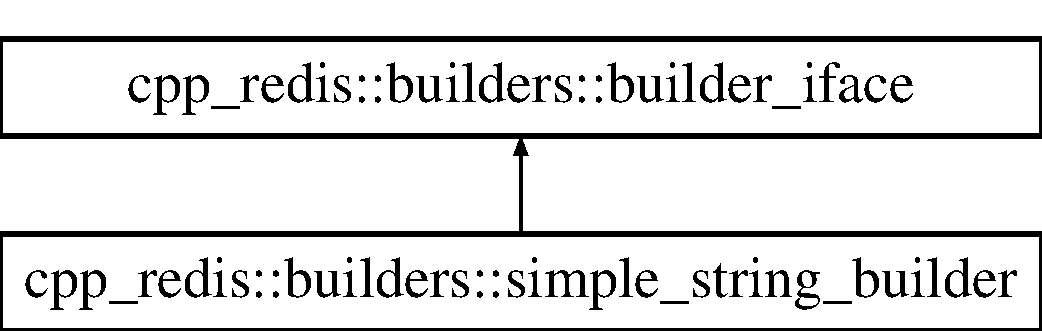
\includegraphics[height=2.000000cm]{classcpp__redis_1_1builders_1_1simple__string__builder}
\end{center}
\end{figure}
\subsection*{Public Member Functions}
\begin{DoxyCompactItemize}
\item 
\hyperlink{classcpp__redis_1_1builders_1_1simple__string__builder_a51fcb7777a78cbd3599aae8896e4d06a}{simple\+\_\+string\+\_\+builder} (void)
\begin{DoxyCompactList}\small\item\em ctor \end{DoxyCompactList}\item 
\hyperlink{classcpp__redis_1_1builders_1_1simple__string__builder_a7b4f012c532535801f9d5fddbb01d675}{$\sim$simple\+\_\+string\+\_\+builder} (void)=default
\begin{DoxyCompactList}\small\item\em dtor \end{DoxyCompactList}\item 
\hyperlink{classcpp__redis_1_1builders_1_1simple__string__builder_a0a17d659e654ee1190c635d3b3093235}{simple\+\_\+string\+\_\+builder} (const \hyperlink{classcpp__redis_1_1builders_1_1simple__string__builder}{simple\+\_\+string\+\_\+builder} \&)=delete
\begin{DoxyCompactList}\small\item\em copy ctor \end{DoxyCompactList}\item 
\hyperlink{classcpp__redis_1_1builders_1_1simple__string__builder}{simple\+\_\+string\+\_\+builder} \& \hyperlink{classcpp__redis_1_1builders_1_1simple__string__builder_afc86dd3148ef0094d08b4282f7cb597d}{operator=} (const \hyperlink{classcpp__redis_1_1builders_1_1simple__string__builder}{simple\+\_\+string\+\_\+builder} \&)=delete
\begin{DoxyCompactList}\small\item\em assignment operator \end{DoxyCompactList}\item 
\hyperlink{classcpp__redis_1_1builders_1_1builder__iface}{builder\+\_\+iface} \& \hyperlink{classcpp__redis_1_1builders_1_1simple__string__builder_a159bb512f0427c4a988742f7cd01035e}{operator$<$$<$} (std\+::string \&data)
\item 
bool \hyperlink{classcpp__redis_1_1builders_1_1simple__string__builder_ad586164caf02b3022b91789cac23a72d}{reply\+\_\+ready} (void) const
\item 
\hyperlink{classcpp__redis_1_1reply}{reply} \hyperlink{classcpp__redis_1_1builders_1_1simple__string__builder_a24ad0968d7d02172a65cf8982c540d51}{get\+\_\+reply} (void) const
\item 
const std\+::string \& \hyperlink{classcpp__redis_1_1builders_1_1simple__string__builder_a539ba8a9234269e57471f1973adc58c2}{get\+\_\+simple\+\_\+string} (void) const
\end{DoxyCompactItemize}
\subsection*{Private Attributes}
\begin{DoxyCompactItemize}
\item 
std\+::string \hyperlink{classcpp__redis_1_1builders_1_1simple__string__builder_acf61d3d6bec2cc33279f4e6ee4cd6f80}{m\+\_\+str}
\item 
bool \hyperlink{classcpp__redis_1_1builders_1_1simple__string__builder_aaf2076e8d2d7154ddc1433aff77a5013}{m\+\_\+reply\+\_\+ready}
\item 
\hyperlink{classcpp__redis_1_1reply}{reply} \hyperlink{classcpp__redis_1_1builders_1_1simple__string__builder_a8a9ee04b09475ab079db623f1d887757}{m\+\_\+reply}
\end{DoxyCompactItemize}


\subsection{Detailed Description}
builder to build redis simplestring replies 

\subsection{Constructor \& Destructor Documentation}
\mbox{\Hypertarget{classcpp__redis_1_1builders_1_1simple__string__builder_a51fcb7777a78cbd3599aae8896e4d06a}\label{classcpp__redis_1_1builders_1_1simple__string__builder_a51fcb7777a78cbd3599aae8896e4d06a}} 
\index{cpp\+\_\+redis\+::builders\+::simple\+\_\+string\+\_\+builder@{cpp\+\_\+redis\+::builders\+::simple\+\_\+string\+\_\+builder}!simple\+\_\+string\+\_\+builder@{simple\+\_\+string\+\_\+builder}}
\index{simple\+\_\+string\+\_\+builder@{simple\+\_\+string\+\_\+builder}!cpp\+\_\+redis\+::builders\+::simple\+\_\+string\+\_\+builder@{cpp\+\_\+redis\+::builders\+::simple\+\_\+string\+\_\+builder}}
\subsubsection{\texorpdfstring{simple\+\_\+string\+\_\+builder()}{simple\_string\_builder()}\hspace{0.1cm}{\footnotesize\ttfamily [1/2]}}
{\footnotesize\ttfamily cpp\+\_\+redis\+::builders\+::simple\+\_\+string\+\_\+builder\+::simple\+\_\+string\+\_\+builder (\begin{DoxyParamCaption}\item[{void}]{ }\end{DoxyParamCaption})}



ctor 

\mbox{\Hypertarget{classcpp__redis_1_1builders_1_1simple__string__builder_a7b4f012c532535801f9d5fddbb01d675}\label{classcpp__redis_1_1builders_1_1simple__string__builder_a7b4f012c532535801f9d5fddbb01d675}} 
\index{cpp\+\_\+redis\+::builders\+::simple\+\_\+string\+\_\+builder@{cpp\+\_\+redis\+::builders\+::simple\+\_\+string\+\_\+builder}!````~simple\+\_\+string\+\_\+builder@{$\sim$simple\+\_\+string\+\_\+builder}}
\index{````~simple\+\_\+string\+\_\+builder@{$\sim$simple\+\_\+string\+\_\+builder}!cpp\+\_\+redis\+::builders\+::simple\+\_\+string\+\_\+builder@{cpp\+\_\+redis\+::builders\+::simple\+\_\+string\+\_\+builder}}
\subsubsection{\texorpdfstring{$\sim$simple\+\_\+string\+\_\+builder()}{~simple\_string\_builder()}}
{\footnotesize\ttfamily cpp\+\_\+redis\+::builders\+::simple\+\_\+string\+\_\+builder\+::$\sim$simple\+\_\+string\+\_\+builder (\begin{DoxyParamCaption}\item[{void}]{ }\end{DoxyParamCaption})\hspace{0.3cm}{\ttfamily [default]}}



dtor 

\mbox{\Hypertarget{classcpp__redis_1_1builders_1_1simple__string__builder_a0a17d659e654ee1190c635d3b3093235}\label{classcpp__redis_1_1builders_1_1simple__string__builder_a0a17d659e654ee1190c635d3b3093235}} 
\index{cpp\+\_\+redis\+::builders\+::simple\+\_\+string\+\_\+builder@{cpp\+\_\+redis\+::builders\+::simple\+\_\+string\+\_\+builder}!simple\+\_\+string\+\_\+builder@{simple\+\_\+string\+\_\+builder}}
\index{simple\+\_\+string\+\_\+builder@{simple\+\_\+string\+\_\+builder}!cpp\+\_\+redis\+::builders\+::simple\+\_\+string\+\_\+builder@{cpp\+\_\+redis\+::builders\+::simple\+\_\+string\+\_\+builder}}
\subsubsection{\texorpdfstring{simple\+\_\+string\+\_\+builder()}{simple\_string\_builder()}\hspace{0.1cm}{\footnotesize\ttfamily [2/2]}}
{\footnotesize\ttfamily cpp\+\_\+redis\+::builders\+::simple\+\_\+string\+\_\+builder\+::simple\+\_\+string\+\_\+builder (\begin{DoxyParamCaption}\item[{const \hyperlink{classcpp__redis_1_1builders_1_1simple__string__builder}{simple\+\_\+string\+\_\+builder} \&}]{ }\end{DoxyParamCaption})\hspace{0.3cm}{\ttfamily [delete]}}



copy ctor 



\subsection{Member Function Documentation}
\mbox{\Hypertarget{classcpp__redis_1_1builders_1_1simple__string__builder_a24ad0968d7d02172a65cf8982c540d51}\label{classcpp__redis_1_1builders_1_1simple__string__builder_a24ad0968d7d02172a65cf8982c540d51}} 
\index{cpp\+\_\+redis\+::builders\+::simple\+\_\+string\+\_\+builder@{cpp\+\_\+redis\+::builders\+::simple\+\_\+string\+\_\+builder}!get\+\_\+reply@{get\+\_\+reply}}
\index{get\+\_\+reply@{get\+\_\+reply}!cpp\+\_\+redis\+::builders\+::simple\+\_\+string\+\_\+builder@{cpp\+\_\+redis\+::builders\+::simple\+\_\+string\+\_\+builder}}
\subsubsection{\texorpdfstring{get\+\_\+reply()}{get\_reply()}}
{\footnotesize\ttfamily \hyperlink{classcpp__redis_1_1reply}{reply} cpp\+\_\+redis\+::builders\+::simple\+\_\+string\+\_\+builder\+::get\+\_\+reply (\begin{DoxyParamCaption}\item[{void}]{ }\end{DoxyParamCaption}) const\hspace{0.3cm}{\ttfamily [virtual]}}

\begin{DoxyReturn}{Returns}
reply object 
\end{DoxyReturn}


Implements \hyperlink{classcpp__redis_1_1builders_1_1builder__iface_afd2ff2c2371c2a486116543b638b9413}{cpp\+\_\+redis\+::builders\+::builder\+\_\+iface}.

\mbox{\Hypertarget{classcpp__redis_1_1builders_1_1simple__string__builder_a539ba8a9234269e57471f1973adc58c2}\label{classcpp__redis_1_1builders_1_1simple__string__builder_a539ba8a9234269e57471f1973adc58c2}} 
\index{cpp\+\_\+redis\+::builders\+::simple\+\_\+string\+\_\+builder@{cpp\+\_\+redis\+::builders\+::simple\+\_\+string\+\_\+builder}!get\+\_\+simple\+\_\+string@{get\+\_\+simple\+\_\+string}}
\index{get\+\_\+simple\+\_\+string@{get\+\_\+simple\+\_\+string}!cpp\+\_\+redis\+::builders\+::simple\+\_\+string\+\_\+builder@{cpp\+\_\+redis\+::builders\+::simple\+\_\+string\+\_\+builder}}
\subsubsection{\texorpdfstring{get\+\_\+simple\+\_\+string()}{get\_simple\_string()}}
{\footnotesize\ttfamily const std\+::string\& cpp\+\_\+redis\+::builders\+::simple\+\_\+string\+\_\+builder\+::get\+\_\+simple\+\_\+string (\begin{DoxyParamCaption}\item[{void}]{ }\end{DoxyParamCaption}) const}

\begin{DoxyReturn}{Returns}
the parsed simple string 
\end{DoxyReturn}
\mbox{\Hypertarget{classcpp__redis_1_1builders_1_1simple__string__builder_a159bb512f0427c4a988742f7cd01035e}\label{classcpp__redis_1_1builders_1_1simple__string__builder_a159bb512f0427c4a988742f7cd01035e}} 
\index{cpp\+\_\+redis\+::builders\+::simple\+\_\+string\+\_\+builder@{cpp\+\_\+redis\+::builders\+::simple\+\_\+string\+\_\+builder}!operator$<$$<$@{operator$<$$<$}}
\index{operator$<$$<$@{operator$<$$<$}!cpp\+\_\+redis\+::builders\+::simple\+\_\+string\+\_\+builder@{cpp\+\_\+redis\+::builders\+::simple\+\_\+string\+\_\+builder}}
\subsubsection{\texorpdfstring{operator$<$$<$()}{operator<<()}}
{\footnotesize\ttfamily \hyperlink{classcpp__redis_1_1builders_1_1builder__iface}{builder\+\_\+iface}\& cpp\+\_\+redis\+::builders\+::simple\+\_\+string\+\_\+builder\+::operator$<$$<$ (\begin{DoxyParamCaption}\item[{std\+::string \&}]{data }\end{DoxyParamCaption})\hspace{0.3cm}{\ttfamily [virtual]}}

take data as parameter which is consumed to build the reply every bytes used to build the reply must be removed from the buffer passed as parameter


\begin{DoxyParams}{Parameters}
{\em data} & data to be consumed \\
\hline
\end{DoxyParams}
\begin{DoxyReturn}{Returns}
current instance 
\end{DoxyReturn}


Implements \hyperlink{classcpp__redis_1_1builders_1_1builder__iface_a9892bbc9c887c31c2742dad4476e2fa6}{cpp\+\_\+redis\+::builders\+::builder\+\_\+iface}.

\mbox{\Hypertarget{classcpp__redis_1_1builders_1_1simple__string__builder_afc86dd3148ef0094d08b4282f7cb597d}\label{classcpp__redis_1_1builders_1_1simple__string__builder_afc86dd3148ef0094d08b4282f7cb597d}} 
\index{cpp\+\_\+redis\+::builders\+::simple\+\_\+string\+\_\+builder@{cpp\+\_\+redis\+::builders\+::simple\+\_\+string\+\_\+builder}!operator=@{operator=}}
\index{operator=@{operator=}!cpp\+\_\+redis\+::builders\+::simple\+\_\+string\+\_\+builder@{cpp\+\_\+redis\+::builders\+::simple\+\_\+string\+\_\+builder}}
\subsubsection{\texorpdfstring{operator=()}{operator=()}}
{\footnotesize\ttfamily \hyperlink{classcpp__redis_1_1builders_1_1simple__string__builder}{simple\+\_\+string\+\_\+builder}\& cpp\+\_\+redis\+::builders\+::simple\+\_\+string\+\_\+builder\+::operator= (\begin{DoxyParamCaption}\item[{const \hyperlink{classcpp__redis_1_1builders_1_1simple__string__builder}{simple\+\_\+string\+\_\+builder} \&}]{ }\end{DoxyParamCaption})\hspace{0.3cm}{\ttfamily [delete]}}



assignment operator 

\mbox{\Hypertarget{classcpp__redis_1_1builders_1_1simple__string__builder_ad586164caf02b3022b91789cac23a72d}\label{classcpp__redis_1_1builders_1_1simple__string__builder_ad586164caf02b3022b91789cac23a72d}} 
\index{cpp\+\_\+redis\+::builders\+::simple\+\_\+string\+\_\+builder@{cpp\+\_\+redis\+::builders\+::simple\+\_\+string\+\_\+builder}!reply\+\_\+ready@{reply\+\_\+ready}}
\index{reply\+\_\+ready@{reply\+\_\+ready}!cpp\+\_\+redis\+::builders\+::simple\+\_\+string\+\_\+builder@{cpp\+\_\+redis\+::builders\+::simple\+\_\+string\+\_\+builder}}
\subsubsection{\texorpdfstring{reply\+\_\+ready()}{reply\_ready()}}
{\footnotesize\ttfamily bool cpp\+\_\+redis\+::builders\+::simple\+\_\+string\+\_\+builder\+::reply\+\_\+ready (\begin{DoxyParamCaption}\item[{void}]{ }\end{DoxyParamCaption}) const\hspace{0.3cm}{\ttfamily [virtual]}}

\begin{DoxyReturn}{Returns}
whether the reply could be built 
\end{DoxyReturn}


Implements \hyperlink{classcpp__redis_1_1builders_1_1builder__iface_a40db9a31d4ea1771777e74146d31e12d}{cpp\+\_\+redis\+::builders\+::builder\+\_\+iface}.



\subsection{Member Data Documentation}
\mbox{\Hypertarget{classcpp__redis_1_1builders_1_1simple__string__builder_a8a9ee04b09475ab079db623f1d887757}\label{classcpp__redis_1_1builders_1_1simple__string__builder_a8a9ee04b09475ab079db623f1d887757}} 
\index{cpp\+\_\+redis\+::builders\+::simple\+\_\+string\+\_\+builder@{cpp\+\_\+redis\+::builders\+::simple\+\_\+string\+\_\+builder}!m\+\_\+reply@{m\+\_\+reply}}
\index{m\+\_\+reply@{m\+\_\+reply}!cpp\+\_\+redis\+::builders\+::simple\+\_\+string\+\_\+builder@{cpp\+\_\+redis\+::builders\+::simple\+\_\+string\+\_\+builder}}
\subsubsection{\texorpdfstring{m\+\_\+reply}{m\_reply}}
{\footnotesize\ttfamily \hyperlink{classcpp__redis_1_1reply}{reply} cpp\+\_\+redis\+::builders\+::simple\+\_\+string\+\_\+builder\+::m\+\_\+reply\hspace{0.3cm}{\ttfamily [private]}}

reply to be built \mbox{\Hypertarget{classcpp__redis_1_1builders_1_1simple__string__builder_aaf2076e8d2d7154ddc1433aff77a5013}\label{classcpp__redis_1_1builders_1_1simple__string__builder_aaf2076e8d2d7154ddc1433aff77a5013}} 
\index{cpp\+\_\+redis\+::builders\+::simple\+\_\+string\+\_\+builder@{cpp\+\_\+redis\+::builders\+::simple\+\_\+string\+\_\+builder}!m\+\_\+reply\+\_\+ready@{m\+\_\+reply\+\_\+ready}}
\index{m\+\_\+reply\+\_\+ready@{m\+\_\+reply\+\_\+ready}!cpp\+\_\+redis\+::builders\+::simple\+\_\+string\+\_\+builder@{cpp\+\_\+redis\+::builders\+::simple\+\_\+string\+\_\+builder}}
\subsubsection{\texorpdfstring{m\+\_\+reply\+\_\+ready}{m\_reply\_ready}}
{\footnotesize\ttfamily bool cpp\+\_\+redis\+::builders\+::simple\+\_\+string\+\_\+builder\+::m\+\_\+reply\+\_\+ready\hspace{0.3cm}{\ttfamily [private]}}

whether the reply is ready or not \mbox{\Hypertarget{classcpp__redis_1_1builders_1_1simple__string__builder_acf61d3d6bec2cc33279f4e6ee4cd6f80}\label{classcpp__redis_1_1builders_1_1simple__string__builder_acf61d3d6bec2cc33279f4e6ee4cd6f80}} 
\index{cpp\+\_\+redis\+::builders\+::simple\+\_\+string\+\_\+builder@{cpp\+\_\+redis\+::builders\+::simple\+\_\+string\+\_\+builder}!m\+\_\+str@{m\+\_\+str}}
\index{m\+\_\+str@{m\+\_\+str}!cpp\+\_\+redis\+::builders\+::simple\+\_\+string\+\_\+builder@{cpp\+\_\+redis\+::builders\+::simple\+\_\+string\+\_\+builder}}
\subsubsection{\texorpdfstring{m\+\_\+str}{m\_str}}
{\footnotesize\ttfamily std\+::string cpp\+\_\+redis\+::builders\+::simple\+\_\+string\+\_\+builder\+::m\+\_\+str\hspace{0.3cm}{\ttfamily [private]}}

parsed simple string 

The documentation for this class was generated from the following file\+:\begin{DoxyCompactItemize}
\item 
includes/cpp\+\_\+redis/builders/\hyperlink{simple__string__builder_8hpp}{simple\+\_\+string\+\_\+builder.\+hpp}\end{DoxyCompactItemize}

\hypertarget{classcpp__redis_1_1subscriber}{}\section{cpp\+\_\+redis\+:\+:subscriber Class Reference}
\label{classcpp__redis_1_1subscriber}\index{cpp\+\_\+redis\+::subscriber@{cpp\+\_\+redis\+::subscriber}}


{\ttfamily \#include $<$subscriber.\+hpp$>$}

\subsection*{Public Types}
\begin{DoxyCompactItemize}
\item 
enum \mbox{\hyperlink{classcpp__redis_1_1subscriber_afc976757efd9d0ac4def6935546a2338}{connect\+\_\+state}} \{ \newline
{\bfseries dropped}, 
{\bfseries start}, 
{\bfseries sleeping}, 
{\bfseries ok}, 
\newline
{\bfseries failed}, 
{\bfseries lookup\+\_\+failed}, 
{\bfseries stopped}
 \}
\item 
\mbox{\Hypertarget{classcpp__redis_1_1subscriber_a7f9e56873e5b96ad9cb2395dadae1a7a}\label{classcpp__redis_1_1subscriber_a7f9e56873e5b96ad9cb2395dadae1a7a}} 
typedef std\+::function$<$ void(const std\+::string \&host, std\+::size\+\_\+t port, \mbox{\hyperlink{classcpp__redis_1_1subscriber_afc976757efd9d0ac4def6935546a2338}{connect\+\_\+state}} status)$>$ \mbox{\hyperlink{classcpp__redis_1_1subscriber_a7f9e56873e5b96ad9cb2395dadae1a7a}{connect\+\_\+callback\+\_\+t}}
\begin{DoxyCompactList}\small\item\em connect handler, called whenever a new connection even occurred \end{DoxyCompactList}\item 
\mbox{\Hypertarget{classcpp__redis_1_1subscriber_a5533ac876d3116911b54ff0dce28f61c}\label{classcpp__redis_1_1subscriber_a5533ac876d3116911b54ff0dce28f61c}} 
typedef std\+::function$<$ void(\mbox{\hyperlink{classcpp__redis_1_1reply}{reply}} \&)$>$ \mbox{\hyperlink{classcpp__redis_1_1subscriber_a5533ac876d3116911b54ff0dce28f61c}{reply\+\_\+callback\+\_\+t}}
\begin{DoxyCompactList}\small\item\em reply callback called whenever a reply is received, takes as parameter the received reply \end{DoxyCompactList}\item 
typedef std\+::function$<$ void(const std\+::string \&, const std\+::string \&)$>$ \mbox{\hyperlink{classcpp__redis_1_1subscriber_a2ac29261280f488dab483866ae875656}{subscribe\+\_\+callback\+\_\+t}}
\item 
typedef std\+::function$<$ void(int64\+\_\+t)$>$ \mbox{\hyperlink{classcpp__redis_1_1subscriber_a19ea39dfabeb19937a9ce4c8d21781b4}{acknowledgement\+\_\+callback\+\_\+t}}
\end{DoxyCompactItemize}
\subsection*{Public Member Functions}
\begin{DoxyCompactItemize}
\item 
\mbox{\Hypertarget{classcpp__redis_1_1subscriber_a7a6cf12c6f12fbc54cd80ceaf7ac4cba}\label{classcpp__redis_1_1subscriber_a7a6cf12c6f12fbc54cd80ceaf7ac4cba}} 
\mbox{\hyperlink{classcpp__redis_1_1subscriber_a7a6cf12c6f12fbc54cd80ceaf7ac4cba}{subscriber}} ()
\begin{DoxyCompactList}\small\item\em ctor \end{DoxyCompactList}\item 
\mbox{\hyperlink{classcpp__redis_1_1subscriber_a66136601f44564842e2c67de2da199af}{subscriber}} (const std\+::shared\+\_\+ptr$<$ \mbox{\hyperlink{classcpp__redis_1_1network_1_1tcp__client__iface}{network\+::tcp\+\_\+client\+\_\+iface}} $>$ \&tcp\+\_\+client)
\item 
\mbox{\Hypertarget{classcpp__redis_1_1subscriber_a24e54cbec0cc6dcae663cf9399740fe7}\label{classcpp__redis_1_1subscriber_a24e54cbec0cc6dcae663cf9399740fe7}} 
\mbox{\hyperlink{classcpp__redis_1_1subscriber_a24e54cbec0cc6dcae663cf9399740fe7}{$\sim$subscriber}} ()
\begin{DoxyCompactList}\small\item\em dtor \end{DoxyCompactList}\item 
\mbox{\Hypertarget{classcpp__redis_1_1subscriber_af5f11532bf727eeb2d4a926bdc775cd7}\label{classcpp__redis_1_1subscriber_af5f11532bf727eeb2d4a926bdc775cd7}} 
\mbox{\hyperlink{classcpp__redis_1_1subscriber_af5f11532bf727eeb2d4a926bdc775cd7}{subscriber}} (const \mbox{\hyperlink{classcpp__redis_1_1subscriber}{subscriber}} \&)=delete
\begin{DoxyCompactList}\small\item\em copy ctor \end{DoxyCompactList}\item 
\mbox{\Hypertarget{classcpp__redis_1_1subscriber_ac60f83e6e915073bda6853baaeb39485}\label{classcpp__redis_1_1subscriber_ac60f83e6e915073bda6853baaeb39485}} 
\mbox{\hyperlink{classcpp__redis_1_1subscriber}{subscriber}} \& \mbox{\hyperlink{classcpp__redis_1_1subscriber_ac60f83e6e915073bda6853baaeb39485}{operator=}} (const \mbox{\hyperlink{classcpp__redis_1_1subscriber}{subscriber}} \&)=delete
\begin{DoxyCompactList}\small\item\em assignment operator \end{DoxyCompactList}\item 
void \mbox{\hyperlink{classcpp__redis_1_1subscriber_a6ae8134a9a9b31d6f2434ec4f6e86d3a}{connect}} (const std\+::string \&host=\char`\"{}127.\+0.\+0.\+1\char`\"{}, std\+::size\+\_\+t port=6379, const \mbox{\hyperlink{classcpp__redis_1_1subscriber_a7f9e56873e5b96ad9cb2395dadae1a7a}{connect\+\_\+callback\+\_\+t}} \&connect\+\_\+callback=nullptr, std\+::uint32\+\_\+t timeout\+\_\+msecs=0, std\+::int32\+\_\+t max\+\_\+reconnects=0, std\+::uint32\+\_\+t reconnect\+\_\+interval\+\_\+msecs=0)
\begin{DoxyCompactList}\small\item\em Connect to redis server. \end{DoxyCompactList}\item 
void \mbox{\hyperlink{classcpp__redis_1_1subscriber_a8fb77a44a1e1f0d99dec639658e2aa7e}{connect}} (const std\+::string \&m_name, const \mbox{\hyperlink{classcpp__redis_1_1subscriber_a7f9e56873e5b96ad9cb2395dadae1a7a}{connect\+\_\+callback\+\_\+t}} \&connect\+\_\+callback=nullptr, std\+::uint32\+\_\+t timeout\+\_\+msecs=0, std\+::int32\+\_\+t max\+\_\+reconnects=0, std\+::uint32\+\_\+t reconnect\+\_\+interval\+\_\+msecs=0)
\begin{DoxyCompactList}\small\item\em Connect to redis server. \end{DoxyCompactList}\item 
bool \mbox{\hyperlink{classcpp__redis_1_1subscriber_af73acfc3c1859e6b32bc9a69856e6e59}{is\+\_\+connected}} () const
\begin{DoxyCompactList}\small\item\em determines client connectivity \end{DoxyCompactList}\item 
void \mbox{\hyperlink{classcpp__redis_1_1subscriber_aad1d0c3c6edb1522eb7b1bdb64b4705d}{disconnect}} (bool wait\+\_\+for\+\_\+removal=false)
\begin{DoxyCompactList}\small\item\em disconnect from redis server \end{DoxyCompactList}\item 
bool \mbox{\hyperlink{classcpp__redis_1_1subscriber_a8df4503f738566d2acab5f080cd44b53}{is\+\_\+reconnecting}} () const
\begin{DoxyCompactList}\small\item\em determines if reconnect is in progress \end{DoxyCompactList}\item 
\mbox{\Hypertarget{classcpp__redis_1_1subscriber_ae93de179d6ea83ece59cf1a30493c3e9}\label{classcpp__redis_1_1subscriber_ae93de179d6ea83ece59cf1a30493c3e9}} 
void \mbox{\hyperlink{classcpp__redis_1_1subscriber_ae93de179d6ea83ece59cf1a30493c3e9}{cancel\+\_\+reconnect}} ()
\begin{DoxyCompactList}\small\item\em stop any reconnect in progress \end{DoxyCompactList}\item 
\mbox{\hyperlink{classcpp__redis_1_1subscriber}{subscriber}} \& \mbox{\hyperlink{classcpp__redis_1_1subscriber_a7b4564fc4dfe356b95aeae4fdb8071c9}{auth}} (const std\+::string \&password, const \mbox{\hyperlink{classcpp__redis_1_1subscriber_a5533ac876d3116911b54ff0dce28f61c}{reply\+\_\+callback\+\_\+t}} \&reply\+\_\+callback=nullptr)
\begin{DoxyCompactList}\small\item\em ability to authenticate on the redis server if necessary this method should not be called repeatedly as the storage of reply\+\_\+callback is N\+OT thread safe (only one reply callback is stored for the subscriber client) calling repeatedly \mbox{\hyperlink{classcpp__redis_1_1subscriber_a7b4564fc4dfe356b95aeae4fdb8071c9}{auth()}} is undefined concerning the execution of the associated callbacks \end{DoxyCompactList}\item 
\mbox{\hyperlink{classcpp__redis_1_1subscriber}{subscriber}} \& \mbox{\hyperlink{classcpp__redis_1_1subscriber_afee579c702182041645a3d3c55de4b9e}{subscribe}} (const std\+::string \&channel, const \mbox{\hyperlink{classcpp__redis_1_1subscriber_a2ac29261280f488dab483866ae875656}{subscribe\+\_\+callback\+\_\+t}} \&callback, const \mbox{\hyperlink{classcpp__redis_1_1subscriber_a19ea39dfabeb19937a9ce4c8d21781b4}{acknowledgement\+\_\+callback\+\_\+t}} \&acknowledgement\+\_\+callback=nullptr)
\item 
\mbox{\hyperlink{classcpp__redis_1_1subscriber}{subscriber}} \& \mbox{\hyperlink{classcpp__redis_1_1subscriber_a52605edb2a85d370680c3c9e1b84fc3b}{psubscribe}} (const std\+::string \&pattern, const \mbox{\hyperlink{classcpp__redis_1_1subscriber_a2ac29261280f488dab483866ae875656}{subscribe\+\_\+callback\+\_\+t}} \&callback, const \mbox{\hyperlink{classcpp__redis_1_1subscriber_a19ea39dfabeb19937a9ce4c8d21781b4}{acknowledgement\+\_\+callback\+\_\+t}} \&acknowledgement\+\_\+callback=nullptr)
\item 
\mbox{\hyperlink{classcpp__redis_1_1subscriber}{subscriber}} \& \mbox{\hyperlink{classcpp__redis_1_1subscriber_a08dffea41cfd5914adfa5a966e0ab292}{unsubscribe}} (const std\+::string \&channel)
\item 
\mbox{\hyperlink{classcpp__redis_1_1subscriber}{subscriber}} \& \mbox{\hyperlink{classcpp__redis_1_1subscriber_a26edc7dcf87ddc8734fac04878ca307a}{punsubscribe}} (const std\+::string \&pattern)
\item 
\mbox{\hyperlink{classcpp__redis_1_1subscriber}{subscriber}} \& \mbox{\hyperlink{classcpp__redis_1_1subscriber_af78a5542315daac42998809eeec30eef}{commit}} ()
\item 
void \mbox{\hyperlink{classcpp__redis_1_1subscriber_a2faf9e9cc9c95e3c0fed148355af84f1}{add\+\_\+sentinel}} (const std\+::string \&host, std\+::size\+\_\+t port, std\+::uint32\+\_\+t timeout\+\_\+msecs=0)
\item 
const \mbox{\hyperlink{classcpp__redis_1_1sentinel}{sentinel}} \& \mbox{\hyperlink{classcpp__redis_1_1subscriber_a0a6212dfba0513508fdc6377f83a0048}{get\+\_\+sentinel}} () const
\item 
\mbox{\hyperlink{classcpp__redis_1_1sentinel}{sentinel}} \& \mbox{\hyperlink{classcpp__redis_1_1subscriber_a4a77354e12a6ef19cad7b0f55b62033c}{get\+\_\+sentinel}} ()
\item 
void \mbox{\hyperlink{classcpp__redis_1_1subscriber_a3f8119bc43a67f8e22369aad529444ba}{clear\+\_\+sentinels}} ()
\end{DoxyCompactItemize}


\subsection{Detailed Description}
The \mbox{\hyperlink{classcpp__redis_1_1subscriber}{cpp\+\_\+redis\+::subscriber}} is meant to be used for P\+U\+B/\+S\+UB communication with the Redis server. Please do not use \mbox{\hyperlink{classcpp__redis_1_1client}{cpp\+\_\+redis\+::client}} to subscribe to some Redis channels as\+:
\begin{DoxyItemize}
\item the behavior is undefined
\item \mbox{\hyperlink{classcpp__redis_1_1client}{cpp\+\_\+redis\+::client}} is not meant for that 
\end{DoxyItemize}

\subsection{Member Typedef Documentation}
\mbox{\Hypertarget{classcpp__redis_1_1subscriber_a19ea39dfabeb19937a9ce4c8d21781b4}\label{classcpp__redis_1_1subscriber_a19ea39dfabeb19937a9ce4c8d21781b4}} 
\index{cpp\+\_\+redis\+::subscriber@{cpp\+\_\+redis\+::subscriber}!acknowledgement\+\_\+callback\+\_\+t@{acknowledgement\+\_\+callback\+\_\+t}}
\index{acknowledgement\+\_\+callback\+\_\+t@{acknowledgement\+\_\+callback\+\_\+t}!cpp\+\_\+redis\+::subscriber@{cpp\+\_\+redis\+::subscriber}}
\subsubsection{\texorpdfstring{acknowledgement\+\_\+callback\+\_\+t}{acknowledgement\_callback\_t}}
{\footnotesize\ttfamily typedef std\+::function$<$void(int64\+\_\+t)$>$ \mbox{\hyperlink{classcpp__redis_1_1subscriber_a19ea39dfabeb19937a9ce4c8d21781b4}{cpp\+\_\+redis\+::subscriber\+::acknowledgement\+\_\+callback\+\_\+t}}}

acknowledgment callback called whenever a subscribe completes takes as parameter the int returned by the redis server (usually the number of channels you are subscribed to) \mbox{\Hypertarget{classcpp__redis_1_1subscriber_a2ac29261280f488dab483866ae875656}\label{classcpp__redis_1_1subscriber_a2ac29261280f488dab483866ae875656}} 
\index{cpp\+\_\+redis\+::subscriber@{cpp\+\_\+redis\+::subscriber}!subscribe\+\_\+callback\+\_\+t@{subscribe\+\_\+callback\+\_\+t}}
\index{subscribe\+\_\+callback\+\_\+t@{subscribe\+\_\+callback\+\_\+t}!cpp\+\_\+redis\+::subscriber@{cpp\+\_\+redis\+::subscriber}}
\subsubsection{\texorpdfstring{subscribe\+\_\+callback\+\_\+t}{subscribe\_callback\_t}}
{\footnotesize\ttfamily typedef std\+::function$<$void(const std\+::string \&, const std\+::string \&)$>$ \mbox{\hyperlink{classcpp__redis_1_1subscriber_a2ac29261280f488dab483866ae875656}{cpp\+\_\+redis\+::subscriber\+::subscribe\+\_\+callback\+\_\+t}}}

subscribe callback, called whenever a new message is published on a subscribed channel takes as parameter the channel and the message 

\subsection{Member Enumeration Documentation}
\mbox{\Hypertarget{classcpp__redis_1_1subscriber_afc976757efd9d0ac4def6935546a2338}\label{classcpp__redis_1_1subscriber_afc976757efd9d0ac4def6935546a2338}} 
\index{cpp\+\_\+redis\+::subscriber@{cpp\+\_\+redis\+::subscriber}!connect\+\_\+state@{connect\+\_\+state}}
\index{connect\+\_\+state@{connect\+\_\+state}!cpp\+\_\+redis\+::subscriber@{cpp\+\_\+redis\+::subscriber}}
\subsubsection{\texorpdfstring{connect\+\_\+state}{connect\_state}}
{\footnotesize\ttfamily enum \mbox{\hyperlink{classcpp__redis_1_1subscriber_afc976757efd9d0ac4def6935546a2338}{cpp\+\_\+redis\+::subscriber\+::connect\+\_\+state}}\hspace{0.3cm}{\ttfamily [strong]}}

high availability (re)connection states
\begin{DoxyItemize}
\item dropped\+: connection has dropped
\item start\+: attempt of connection has started
\item sleeping\+: sleep between two attempts
\item ok\+: connected
\item failed\+: failed to connect
\item lookup failed\+: failed to retrieve master sentinel
\item stopped\+: stop to try to reconnect 
\end{DoxyItemize}

\subsection{Constructor \& Destructor Documentation}
\mbox{\Hypertarget{classcpp__redis_1_1subscriber_a66136601f44564842e2c67de2da199af}\label{classcpp__redis_1_1subscriber_a66136601f44564842e2c67de2da199af}} 
\index{cpp\+\_\+redis\+::subscriber@{cpp\+\_\+redis\+::subscriber}!subscriber@{subscriber}}
\index{subscriber@{subscriber}!cpp\+\_\+redis\+::subscriber@{cpp\+\_\+redis\+::subscriber}}
\subsubsection{\texorpdfstring{subscriber()}{subscriber()}}
{\footnotesize\ttfamily cpp\+\_\+redis\+::subscriber\+::subscriber (\begin{DoxyParamCaption}\item[{const std\+::shared\+\_\+ptr$<$ \mbox{\hyperlink{classcpp__redis_1_1network_1_1tcp__client__iface}{network\+::tcp\+\_\+client\+\_\+iface}} $>$ \&}]{tcp\+\_\+client }\end{DoxyParamCaption})\hspace{0.3cm}{\ttfamily [explicit]}}

custom ctor to specify custom tcp\+\_\+client


\begin{DoxyParams}{Parameters}
{\em tcp\+\_\+client} & tcp client to be used for network communications \\
\hline
\end{DoxyParams}


\subsection{Member Function Documentation}
\mbox{\Hypertarget{classcpp__redis_1_1subscriber_a2faf9e9cc9c95e3c0fed148355af84f1}\label{classcpp__redis_1_1subscriber_a2faf9e9cc9c95e3c0fed148355af84f1}} 
\index{cpp\+\_\+redis\+::subscriber@{cpp\+\_\+redis\+::subscriber}!add\+\_\+sentinel@{add\+\_\+sentinel}}
\index{add\+\_\+sentinel@{add\+\_\+sentinel}!cpp\+\_\+redis\+::subscriber@{cpp\+\_\+redis\+::subscriber}}
\subsubsection{\texorpdfstring{add\+\_\+sentinel()}{add\_sentinel()}}
{\footnotesize\ttfamily void cpp\+\_\+redis\+::subscriber\+::add\+\_\+sentinel (\begin{DoxyParamCaption}\item[{const std\+::string \&}]{host,  }\item[{std\+::size\+\_\+t}]{port,  }\item[{std\+::uint32\+\_\+t}]{timeout\+\_\+msecs = {\ttfamily 0} }\end{DoxyParamCaption})}

add a sentinel definition. Required for \mbox{\hyperlink{classcpp__redis_1_1subscriber_a6ae8134a9a9b31d6f2434ec4f6e86d3a}{connect()}} or get\+\_\+master\+\_\+addr\+\_\+by\+\_\+m_name() when autoconnect is enabled.


\begin{DoxyParams}{Parameters}
{\em host} & sentinel host \\
\hline
{\em port} & sentinel port \\
\hline
{\em timeout\+\_\+msecs} & maximum time to connect \\
\hline
\end{DoxyParams}
\mbox{\Hypertarget{classcpp__redis_1_1subscriber_a7b4564fc4dfe356b95aeae4fdb8071c9}\label{classcpp__redis_1_1subscriber_a7b4564fc4dfe356b95aeae4fdb8071c9}} 
\index{cpp\+\_\+redis\+::subscriber@{cpp\+\_\+redis\+::subscriber}!auth@{auth}}
\index{auth@{auth}!cpp\+\_\+redis\+::subscriber@{cpp\+\_\+redis\+::subscriber}}
\subsubsection{\texorpdfstring{auth()}{auth()}}
{\footnotesize\ttfamily \mbox{\hyperlink{classcpp__redis_1_1subscriber}{subscriber}}\& cpp\+\_\+redis\+::subscriber\+::auth (\begin{DoxyParamCaption}\item[{const std\+::string \&}]{password,  }\item[{const \mbox{\hyperlink{classcpp__redis_1_1subscriber_a5533ac876d3116911b54ff0dce28f61c}{reply\+\_\+callback\+\_\+t}} \&}]{reply\+\_\+callback = {\ttfamily nullptr} }\end{DoxyParamCaption})}



ability to authenticate on the redis server if necessary this method should not be called repeatedly as the storage of reply\+\_\+callback is N\+OT thread safe (only one reply callback is stored for the subscriber client) calling repeatedly \mbox{\hyperlink{classcpp__redis_1_1subscriber_a7b4564fc4dfe356b95aeae4fdb8071c9}{auth()}} is undefined concerning the execution of the associated callbacks 


\begin{DoxyParams}{Parameters}
{\em password} & password to be used for authentication \\
\hline
{\em reply\+\_\+callback} & callback to be called on auth completion (nullable) \\
\hline
\end{DoxyParams}
\begin{DoxyReturn}{Returns}
current instance 
\end{DoxyReturn}
\mbox{\Hypertarget{classcpp__redis_1_1subscriber_a3f8119bc43a67f8e22369aad529444ba}\label{classcpp__redis_1_1subscriber_a3f8119bc43a67f8e22369aad529444ba}} 
\index{cpp\+\_\+redis\+::subscriber@{cpp\+\_\+redis\+::subscriber}!clear\+\_\+sentinels@{clear\+\_\+sentinels}}
\index{clear\+\_\+sentinels@{clear\+\_\+sentinels}!cpp\+\_\+redis\+::subscriber@{cpp\+\_\+redis\+::subscriber}}
\subsubsection{\texorpdfstring{clear\+\_\+sentinels()}{clear\_sentinels()}}
{\footnotesize\ttfamily void cpp\+\_\+redis\+::subscriber\+::clear\+\_\+sentinels (\begin{DoxyParamCaption}{ }\end{DoxyParamCaption})}

clear all existing sentinels. \mbox{\Hypertarget{classcpp__redis_1_1subscriber_af78a5542315daac42998809eeec30eef}\label{classcpp__redis_1_1subscriber_af78a5542315daac42998809eeec30eef}} 
\index{cpp\+\_\+redis\+::subscriber@{cpp\+\_\+redis\+::subscriber}!commit@{commit}}
\index{commit@{commit}!cpp\+\_\+redis\+::subscriber@{cpp\+\_\+redis\+::subscriber}}
\subsubsection{\texorpdfstring{commit()}{commit()}}
{\footnotesize\ttfamily \mbox{\hyperlink{classcpp__redis_1_1subscriber}{subscriber}}\& cpp\+\_\+redis\+::subscriber\+::commit (\begin{DoxyParamCaption}{ }\end{DoxyParamCaption})}

commit pipelined transaction that is, send to the network all commands pipelined by calling send() / \mbox{\hyperlink{classcpp__redis_1_1subscriber_afee579c702182041645a3d3c55de4b9e}{subscribe()}} / ...

\begin{DoxyReturn}{Returns}
current instance 
\end{DoxyReturn}
\mbox{\Hypertarget{classcpp__redis_1_1subscriber_a6ae8134a9a9b31d6f2434ec4f6e86d3a}\label{classcpp__redis_1_1subscriber_a6ae8134a9a9b31d6f2434ec4f6e86d3a}} 
\index{cpp\+\_\+redis\+::subscriber@{cpp\+\_\+redis\+::subscriber}!connect@{connect}}
\index{connect@{connect}!cpp\+\_\+redis\+::subscriber@{cpp\+\_\+redis\+::subscriber}}
\subsubsection{\texorpdfstring{connect()}{connect()}\hspace{0.1cm}{\footnotesize\ttfamily [1/2]}}
{\footnotesize\ttfamily void cpp\+\_\+redis\+::subscriber\+::connect (\begin{DoxyParamCaption}\item[{const std\+::string \&}]{host = {\ttfamily \char`\"{}127.0.0.1\char`\"{}},  }\item[{std\+::size\+\_\+t}]{port = {\ttfamily 6379},  }\item[{const \mbox{\hyperlink{classcpp__redis_1_1subscriber_a7f9e56873e5b96ad9cb2395dadae1a7a}{connect\+\_\+callback\+\_\+t}} \&}]{connect\+\_\+callback = {\ttfamily nullptr},  }\item[{std\+::uint32\+\_\+t}]{timeout\+\_\+msecs = {\ttfamily 0},  }\item[{std\+::int32\+\_\+t}]{max\+\_\+reconnects = {\ttfamily 0},  }\item[{std\+::uint32\+\_\+t}]{reconnect\+\_\+interval\+\_\+msecs = {\ttfamily 0} }\end{DoxyParamCaption})}



Connect to redis server. 


\begin{DoxyParams}{Parameters}
{\em host} & host to be connected to \\
\hline
{\em port} & port to be connected to \\
\hline
{\em connect\+\_\+callback} & connect handler to be called on connect events (may be null) \\
\hline
{\em timeout\+\_\+msecs} & maximum time to connect \\
\hline
{\em max\+\_\+reconnects} & maximum attempts of reconnection if connection dropped \\
\hline
{\em reconnect\+\_\+interval\+\_\+msecs} & time between two attempts of reconnection \\
\hline
\end{DoxyParams}
\mbox{\Hypertarget{classcpp__redis_1_1subscriber_a8fb77a44a1e1f0d99dec639658e2aa7e}\label{classcpp__redis_1_1subscriber_a8fb77a44a1e1f0d99dec639658e2aa7e}} 
\index{cpp\+\_\+redis\+::subscriber@{cpp\+\_\+redis\+::subscriber}!connect@{connect}}
\index{connect@{connect}!cpp\+\_\+redis\+::subscriber@{cpp\+\_\+redis\+::subscriber}}
\subsubsection{\texorpdfstring{connect()}{connect()}\hspace{0.1cm}{\footnotesize\ttfamily [2/2]}}
{\footnotesize\ttfamily void cpp\+\_\+redis\+::subscriber\+::connect (\begin{DoxyParamCaption}\item[{const std\+::string \&}]{m_name,  }\item[{const \mbox{\hyperlink{classcpp__redis_1_1subscriber_a7f9e56873e5b96ad9cb2395dadae1a7a}{connect\+\_\+callback\+\_\+t}} \&}]{connect\+\_\+callback = {\ttfamily nullptr},  }\item[{std\+::uint32\+\_\+t}]{timeout\+\_\+msecs = {\ttfamily 0},  }\item[{std\+::int32\+\_\+t}]{max\+\_\+reconnects = {\ttfamily 0},  }\item[{std\+::uint32\+\_\+t}]{reconnect\+\_\+interval\+\_\+msecs = {\ttfamily 0} }\end{DoxyParamCaption})}



Connect to redis server. 


\begin{DoxyParams}{Parameters}
{\em m_name} & sentinel m_name \\
\hline
{\em connect\+\_\+callback} & connect handler to be called on connect events (may be null) \\
\hline
{\em timeout\+\_\+msecs} & maximum time to connect \\
\hline
{\em max\+\_\+reconnects} & maximum attempts of reconnection if connection dropped \\
\hline
{\em reconnect\+\_\+interval\+\_\+msecs} & time between two attempts of reconnection \\
\hline
\end{DoxyParams}
\mbox{\Hypertarget{classcpp__redis_1_1subscriber_aad1d0c3c6edb1522eb7b1bdb64b4705d}\label{classcpp__redis_1_1subscriber_aad1d0c3c6edb1522eb7b1bdb64b4705d}} 
\index{cpp\+\_\+redis\+::subscriber@{cpp\+\_\+redis\+::subscriber}!disconnect@{disconnect}}
\index{disconnect@{disconnect}!cpp\+\_\+redis\+::subscriber@{cpp\+\_\+redis\+::subscriber}}
\subsubsection{\texorpdfstring{disconnect()}{disconnect()}}
{\footnotesize\ttfamily void cpp\+\_\+redis\+::subscriber\+::disconnect (\begin{DoxyParamCaption}\item[{bool}]{wait\+\_\+for\+\_\+removal = {\ttfamily false} }\end{DoxyParamCaption})}



disconnect from redis server 


\begin{DoxyParams}{Parameters}
{\em wait\+\_\+for\+\_\+removal} & when set to true, disconnect blocks until the underlying T\+CP client has been effectively removed from the io\+\_\+service and that all the underlying callbacks have completed. \\
\hline
\end{DoxyParams}
\mbox{\Hypertarget{classcpp__redis_1_1subscriber_a0a6212dfba0513508fdc6377f83a0048}\label{classcpp__redis_1_1subscriber_a0a6212dfba0513508fdc6377f83a0048}} 
\index{cpp\+\_\+redis\+::subscriber@{cpp\+\_\+redis\+::subscriber}!get\+\_\+sentinel@{get\+\_\+sentinel}}
\index{get\+\_\+sentinel@{get\+\_\+sentinel}!cpp\+\_\+redis\+::subscriber@{cpp\+\_\+redis\+::subscriber}}
\subsubsection{\texorpdfstring{get\+\_\+sentinel()}{get\_sentinel()}\hspace{0.1cm}{\footnotesize\ttfamily [1/2]}}
{\footnotesize\ttfamily const \mbox{\hyperlink{classcpp__redis_1_1sentinel}{sentinel}}\& cpp\+\_\+redis\+::subscriber\+::get\+\_\+sentinel (\begin{DoxyParamCaption}{ }\end{DoxyParamCaption}) const}

retrieve sentinel for current client

\begin{DoxyReturn}{Returns}
sentinel associated to current client 
\end{DoxyReturn}
\mbox{\Hypertarget{classcpp__redis_1_1subscriber_a4a77354e12a6ef19cad7b0f55b62033c}\label{classcpp__redis_1_1subscriber_a4a77354e12a6ef19cad7b0f55b62033c}} 
\index{cpp\+\_\+redis\+::subscriber@{cpp\+\_\+redis\+::subscriber}!get\+\_\+sentinel@{get\+\_\+sentinel}}
\index{get\+\_\+sentinel@{get\+\_\+sentinel}!cpp\+\_\+redis\+::subscriber@{cpp\+\_\+redis\+::subscriber}}
\subsubsection{\texorpdfstring{get\+\_\+sentinel()}{get\_sentinel()}\hspace{0.1cm}{\footnotesize\ttfamily [2/2]}}
{\footnotesize\ttfamily \mbox{\hyperlink{classcpp__redis_1_1sentinel}{sentinel}}\& cpp\+\_\+redis\+::subscriber\+::get\+\_\+sentinel (\begin{DoxyParamCaption}{ }\end{DoxyParamCaption})}

retrieve sentinel for current client non-\/const version

\begin{DoxyReturn}{Returns}
sentinel associated to current client 
\end{DoxyReturn}
\mbox{\Hypertarget{classcpp__redis_1_1subscriber_af73acfc3c1859e6b32bc9a69856e6e59}\label{classcpp__redis_1_1subscriber_af73acfc3c1859e6b32bc9a69856e6e59}} 
\index{cpp\+\_\+redis\+::subscriber@{cpp\+\_\+redis\+::subscriber}!is\+\_\+connected@{is\+\_\+connected}}
\index{is\+\_\+connected@{is\+\_\+connected}!cpp\+\_\+redis\+::subscriber@{cpp\+\_\+redis\+::subscriber}}
\subsubsection{\texorpdfstring{is\+\_\+connected()}{is\_connected()}}
{\footnotesize\ttfamily bool cpp\+\_\+redis\+::subscriber\+::is\+\_\+connected (\begin{DoxyParamCaption}{ }\end{DoxyParamCaption}) const}



determines client connectivity 

\begin{DoxyReturn}{Returns}
whether we are connected to the redis server 
\end{DoxyReturn}
\mbox{\Hypertarget{classcpp__redis_1_1subscriber_a8df4503f738566d2acab5f080cd44b53}\label{classcpp__redis_1_1subscriber_a8df4503f738566d2acab5f080cd44b53}} 
\index{cpp\+\_\+redis\+::subscriber@{cpp\+\_\+redis\+::subscriber}!is\+\_\+reconnecting@{is\+\_\+reconnecting}}
\index{is\+\_\+reconnecting@{is\+\_\+reconnecting}!cpp\+\_\+redis\+::subscriber@{cpp\+\_\+redis\+::subscriber}}
\subsubsection{\texorpdfstring{is\+\_\+reconnecting()}{is\_reconnecting()}}
{\footnotesize\ttfamily bool cpp\+\_\+redis\+::subscriber\+::is\+\_\+reconnecting (\begin{DoxyParamCaption}{ }\end{DoxyParamCaption}) const}



determines if reconnect is in progress 

\begin{DoxyReturn}{Returns}
whether an attempt to reconnect is in progress 
\end{DoxyReturn}
\mbox{\Hypertarget{classcpp__redis_1_1subscriber_a52605edb2a85d370680c3c9e1b84fc3b}\label{classcpp__redis_1_1subscriber_a52605edb2a85d370680c3c9e1b84fc3b}} 
\index{cpp\+\_\+redis\+::subscriber@{cpp\+\_\+redis\+::subscriber}!psubscribe@{psubscribe}}
\index{psubscribe@{psubscribe}!cpp\+\_\+redis\+::subscriber@{cpp\+\_\+redis\+::subscriber}}
\subsubsection{\texorpdfstring{psubscribe()}{psubscribe()}}
{\footnotesize\ttfamily \mbox{\hyperlink{classcpp__redis_1_1subscriber}{subscriber}}\& cpp\+\_\+redis\+::subscriber\+::psubscribe (\begin{DoxyParamCaption}\item[{const std\+::string \&}]{pattern,  }\item[{const \mbox{\hyperlink{classcpp__redis_1_1subscriber_a2ac29261280f488dab483866ae875656}{subscribe\+\_\+callback\+\_\+t}} \&}]{callback,  }\item[{const \mbox{\hyperlink{classcpp__redis_1_1subscriber_a19ea39dfabeb19937a9ce4c8d21781b4}{acknowledgement\+\_\+callback\+\_\+t}} \&}]{acknowledgement\+\_\+callback = {\ttfamily nullptr} }\end{DoxyParamCaption})}

P\+Subscribes to the given channel and\+:
\begin{DoxyItemize}
\item calls acknowledgement\+\_\+callback once the server has acknowledged about the subscription.
\item calls subscribe\+\_\+callback each time a message is published on this channel. The command is not effectively sent immediately but stored in an internal buffer until \mbox{\hyperlink{classcpp__redis_1_1subscriber_af78a5542315daac42998809eeec30eef}{commit()}} is called.
\end{DoxyItemize}


\begin{DoxyParams}{Parameters}
{\em pattern} & pattern to psubscribe \\
\hline
{\em callback} & callback to be called whenever a message is received for this pattern \\
\hline
{\em acknowledgement\+\_\+callback} & callback to be called on subscription completion (nullable) \\
\hline
\end{DoxyParams}
\begin{DoxyReturn}{Returns}
current instance 
\end{DoxyReturn}
\mbox{\Hypertarget{classcpp__redis_1_1subscriber_a26edc7dcf87ddc8734fac04878ca307a}\label{classcpp__redis_1_1subscriber_a26edc7dcf87ddc8734fac04878ca307a}} 
\index{cpp\+\_\+redis\+::subscriber@{cpp\+\_\+redis\+::subscriber}!punsubscribe@{punsubscribe}}
\index{punsubscribe@{punsubscribe}!cpp\+\_\+redis\+::subscriber@{cpp\+\_\+redis\+::subscriber}}
\subsubsection{\texorpdfstring{punsubscribe()}{punsubscribe()}}
{\footnotesize\ttfamily \mbox{\hyperlink{classcpp__redis_1_1subscriber}{subscriber}}\& cpp\+\_\+redis\+::subscriber\+::punsubscribe (\begin{DoxyParamCaption}\item[{const std\+::string \&}]{pattern }\end{DoxyParamCaption})}

punsubscribe from the given pattern The command is not effectively sent immediately, but stored inside an internal buffer until \mbox{\hyperlink{classcpp__redis_1_1subscriber_af78a5542315daac42998809eeec30eef}{commit()}} is called.


\begin{DoxyParams}{Parameters}
{\em pattern} & pattern to punsubscribe from \\
\hline
\end{DoxyParams}
\begin{DoxyReturn}{Returns}
current instance 
\end{DoxyReturn}
\mbox{\Hypertarget{classcpp__redis_1_1subscriber_afee579c702182041645a3d3c55de4b9e}\label{classcpp__redis_1_1subscriber_afee579c702182041645a3d3c55de4b9e}} 
\index{cpp\+\_\+redis\+::subscriber@{cpp\+\_\+redis\+::subscriber}!subscribe@{subscribe}}
\index{subscribe@{subscribe}!cpp\+\_\+redis\+::subscriber@{cpp\+\_\+redis\+::subscriber}}
\subsubsection{\texorpdfstring{subscribe()}{subscribe()}}
{\footnotesize\ttfamily \mbox{\hyperlink{classcpp__redis_1_1subscriber}{subscriber}}\& cpp\+\_\+redis\+::subscriber\+::subscribe (\begin{DoxyParamCaption}\item[{const std\+::string \&}]{channel,  }\item[{const \mbox{\hyperlink{classcpp__redis_1_1subscriber_a2ac29261280f488dab483866ae875656}{subscribe\+\_\+callback\+\_\+t}} \&}]{callback,  }\item[{const \mbox{\hyperlink{classcpp__redis_1_1subscriber_a19ea39dfabeb19937a9ce4c8d21781b4}{acknowledgement\+\_\+callback\+\_\+t}} \&}]{acknowledgement\+\_\+callback = {\ttfamily nullptr} }\end{DoxyParamCaption})}

Subscribes to the given channel and\+:
\begin{DoxyItemize}
\item calls acknowledgement\+\_\+callback once the server has acknowledged about the subscription.
\item calls subscribe\+\_\+callback each time a message is published on this channel. The command is not effectively sent immediately but stored in an internal buffer until \mbox{\hyperlink{classcpp__redis_1_1subscriber_af78a5542315daac42998809eeec30eef}{commit()}} is called.
\end{DoxyItemize}


\begin{DoxyParams}{Parameters}
{\em channel} & channel to subscribe \\
\hline
{\em callback} & callback to be called whenever a message is received for this channel \\
\hline
{\em acknowledgement\+\_\+callback} & callback to be called on subscription completion (nullable) \\
\hline
\end{DoxyParams}
\begin{DoxyReturn}{Returns}
current instance 
\end{DoxyReturn}
\mbox{\Hypertarget{classcpp__redis_1_1subscriber_a08dffea41cfd5914adfa5a966e0ab292}\label{classcpp__redis_1_1subscriber_a08dffea41cfd5914adfa5a966e0ab292}} 
\index{cpp\+\_\+redis\+::subscriber@{cpp\+\_\+redis\+::subscriber}!unsubscribe@{unsubscribe}}
\index{unsubscribe@{unsubscribe}!cpp\+\_\+redis\+::subscriber@{cpp\+\_\+redis\+::subscriber}}
\subsubsection{\texorpdfstring{unsubscribe()}{unsubscribe()}}
{\footnotesize\ttfamily \mbox{\hyperlink{classcpp__redis_1_1subscriber}{subscriber}}\& cpp\+\_\+redis\+::subscriber\+::unsubscribe (\begin{DoxyParamCaption}\item[{const std\+::string \&}]{channel }\end{DoxyParamCaption})}

unsubscribe from the given channel The command is not effectively sent immediately, but stored inside an internal buffer until \mbox{\hyperlink{classcpp__redis_1_1subscriber_af78a5542315daac42998809eeec30eef}{commit()}} is called.


\begin{DoxyParams}{Parameters}
{\em channel} & channel to unsubscribe from \\
\hline
\end{DoxyParams}
\begin{DoxyReturn}{Returns}
current instance 
\end{DoxyReturn}


The documentation for this class was generated from the following file\+:\begin{DoxyCompactItemize}
\item 
includes/cpp\+\_\+redis/core/subscriber.\+hpp\end{DoxyCompactItemize}

\hypertarget{classcpp__redis_1_1network_1_1tcp__client}{}\section{cpp\+\_\+redis\+:\+:network\+:\+:tcp\+\_\+client Class Reference}
\label{classcpp__redis_1_1network_1_1tcp__client}\index{cpp\+\_\+redis\+::network\+::tcp\+\_\+client@{cpp\+\_\+redis\+::network\+::tcp\+\_\+client}}


{\ttfamily \#include $<$tcp\+\_\+client.\+hpp$>$}

Inheritance diagram for cpp\+\_\+redis\+:\+:network\+:\+:tcp\+\_\+client\+:\begin{figure}[H]
\begin{center}
\leavevmode
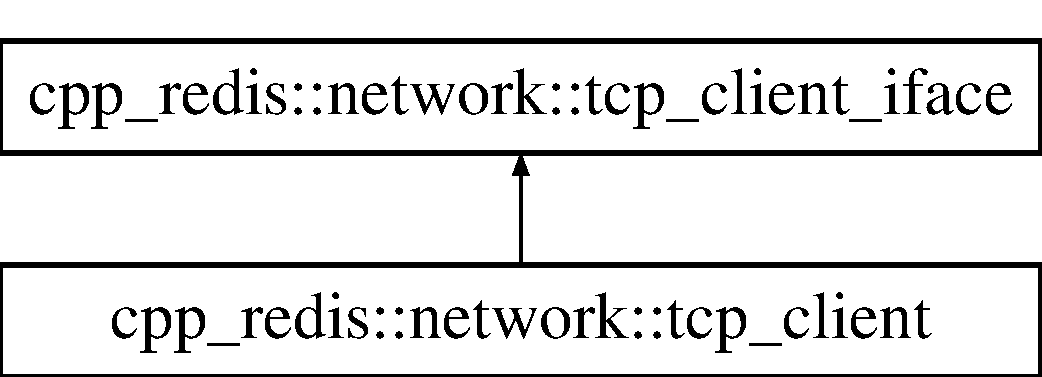
\includegraphics[height=2.000000cm]{classcpp__redis_1_1network_1_1tcp__client}
\end{center}
\end{figure}
\subsection*{Public Member Functions}
\begin{DoxyCompactItemize}
\item 
\mbox{\Hypertarget{classcpp__redis_1_1network_1_1tcp__client_a8cbad07ca636e9d60dafc0e5cac8106d}\label{classcpp__redis_1_1network_1_1tcp__client_a8cbad07ca636e9d60dafc0e5cac8106d}} 
\hyperlink{classcpp__redis_1_1network_1_1tcp__client_a8cbad07ca636e9d60dafc0e5cac8106d}{tcp\+\_\+client} (void)=default
\begin{DoxyCompactList}\small\item\em ctor \end{DoxyCompactList}\item 
\mbox{\Hypertarget{classcpp__redis_1_1network_1_1tcp__client_af859036bbc7e5ec9149c1410a1a66f09}\label{classcpp__redis_1_1network_1_1tcp__client_af859036bbc7e5ec9149c1410a1a66f09}} 
\hyperlink{classcpp__redis_1_1network_1_1tcp__client_af859036bbc7e5ec9149c1410a1a66f09}{$\sim$tcp\+\_\+client} (void)=default
\begin{DoxyCompactList}\small\item\em dtor \end{DoxyCompactList}\item 
void \hyperlink{classcpp__redis_1_1network_1_1tcp__client_a5808c0569980d83479f755ac55a12dfb}{connect} (const std\+::string \&addr, std\+::uint32\+\_\+t port, std\+::uint32\+\_\+t timeout\+\_\+msecs)
\item 
void \hyperlink{classcpp__redis_1_1network_1_1tcp__client_a88f49c4e32d59855a62296fb74136a44}{disconnect} (bool wait\+\_\+for\+\_\+removal=false)
\item 
bool \hyperlink{classcpp__redis_1_1network_1_1tcp__client_a0a636ca6bd59425bf22416a1c7694f65}{is\+\_\+connected} (void) const
\item 
void \hyperlink{classcpp__redis_1_1network_1_1tcp__client_aa56fc49540d67c5c05b3dda3aaff8a0f}{set\+\_\+nb\+\_\+workers} (std\+::size\+\_\+t nb\+\_\+threads)
\item 
void \hyperlink{classcpp__redis_1_1network_1_1tcp__client_a5eed4225fcd01e3108580d863c94c2cc}{async\+\_\+read} (\hyperlink{structcpp__redis_1_1network_1_1tcp__client__iface_1_1read__request}{read\+\_\+request} \&request)
\item 
void \hyperlink{classcpp__redis_1_1network_1_1tcp__client_a6d15785b71776cd85426c9634cb446f0}{async\+\_\+write} (\hyperlink{structcpp__redis_1_1network_1_1tcp__client__iface_1_1write__request}{write\+\_\+request} \&request)
\item 
void \hyperlink{classcpp__redis_1_1network_1_1tcp__client_a24ccdf6dc467aac13cb832a395adb38d}{set\+\_\+on\+\_\+disconnection\+\_\+handler} (const \hyperlink{classcpp__redis_1_1network_1_1tcp__client__iface_a9a7d5942205db8be03da581a848b8ec0}{disconnection\+\_\+handler\+\_\+t} \&disconnection\+\_\+handler)
\end{DoxyCompactItemize}
\subsection*{Additional Inherited Members}


\subsection{Detailed Description}
implementation of the \hyperlink{classcpp__redis_1_1network_1_1tcp__client__iface}{tcp\+\_\+client\+\_\+iface} based on tacopie networking library 

\subsection{Member Function Documentation}
\mbox{\Hypertarget{classcpp__redis_1_1network_1_1tcp__client_a5eed4225fcd01e3108580d863c94c2cc}\label{classcpp__redis_1_1network_1_1tcp__client_a5eed4225fcd01e3108580d863c94c2cc}} 
\index{cpp\+\_\+redis\+::network\+::tcp\+\_\+client@{cpp\+\_\+redis\+::network\+::tcp\+\_\+client}!async\+\_\+read@{async\+\_\+read}}
\index{async\+\_\+read@{async\+\_\+read}!cpp\+\_\+redis\+::network\+::tcp\+\_\+client@{cpp\+\_\+redis\+::network\+::tcp\+\_\+client}}
\subsubsection{\texorpdfstring{async\+\_\+read()}{async\_read()}}
{\footnotesize\ttfamily void cpp\+\_\+redis\+::network\+::tcp\+\_\+client\+::async\+\_\+read (\begin{DoxyParamCaption}\item[{\hyperlink{structcpp__redis_1_1network_1_1tcp__client__iface_1_1read__request}{read\+\_\+request} \&}]{request }\end{DoxyParamCaption})\hspace{0.3cm}{\ttfamily [virtual]}}

async read operation


\begin{DoxyParams}{Parameters}
{\em request} & information about what should be read and what should be done after completion \\
\hline
\end{DoxyParams}


Implements \hyperlink{classcpp__redis_1_1network_1_1tcp__client__iface_ae1f9fa87002273a0caf340407bb68ade}{cpp\+\_\+redis\+::network\+::tcp\+\_\+client\+\_\+iface}.

\mbox{\Hypertarget{classcpp__redis_1_1network_1_1tcp__client_a6d15785b71776cd85426c9634cb446f0}\label{classcpp__redis_1_1network_1_1tcp__client_a6d15785b71776cd85426c9634cb446f0}} 
\index{cpp\+\_\+redis\+::network\+::tcp\+\_\+client@{cpp\+\_\+redis\+::network\+::tcp\+\_\+client}!async\+\_\+write@{async\+\_\+write}}
\index{async\+\_\+write@{async\+\_\+write}!cpp\+\_\+redis\+::network\+::tcp\+\_\+client@{cpp\+\_\+redis\+::network\+::tcp\+\_\+client}}
\subsubsection{\texorpdfstring{async\+\_\+write()}{async\_write()}}
{\footnotesize\ttfamily void cpp\+\_\+redis\+::network\+::tcp\+\_\+client\+::async\+\_\+write (\begin{DoxyParamCaption}\item[{\hyperlink{structcpp__redis_1_1network_1_1tcp__client__iface_1_1write__request}{write\+\_\+request} \&}]{request }\end{DoxyParamCaption})\hspace{0.3cm}{\ttfamily [virtual]}}

async write operation


\begin{DoxyParams}{Parameters}
{\em request} & information about what should be written and what should be done after completion \\
\hline
\end{DoxyParams}


Implements \hyperlink{classcpp__redis_1_1network_1_1tcp__client__iface_a9cd01e8a68479456d15d6435ffad9b92}{cpp\+\_\+redis\+::network\+::tcp\+\_\+client\+\_\+iface}.

\mbox{\Hypertarget{classcpp__redis_1_1network_1_1tcp__client_a5808c0569980d83479f755ac55a12dfb}\label{classcpp__redis_1_1network_1_1tcp__client_a5808c0569980d83479f755ac55a12dfb}} 
\index{cpp\+\_\+redis\+::network\+::tcp\+\_\+client@{cpp\+\_\+redis\+::network\+::tcp\+\_\+client}!connect@{connect}}
\index{connect@{connect}!cpp\+\_\+redis\+::network\+::tcp\+\_\+client@{cpp\+\_\+redis\+::network\+::tcp\+\_\+client}}
\subsubsection{\texorpdfstring{connect()}{connect()}}
{\footnotesize\ttfamily void cpp\+\_\+redis\+::network\+::tcp\+\_\+client\+::connect (\begin{DoxyParamCaption}\item[{const std\+::string \&}]{addr,  }\item[{std\+::uint32\+\_\+t}]{port,  }\item[{std\+::uint32\+\_\+t}]{timeout\+\_\+msecs }\end{DoxyParamCaption})\hspace{0.3cm}{\ttfamily [virtual]}}

start the tcp client


\begin{DoxyParams}{Parameters}
{\em addr} & host to be connected to \\
\hline
{\em port} & port to be connected to \\
\hline
{\em timeout\+\_\+msecs} & max time to connect in ms \\
\hline
\end{DoxyParams}


Implements \hyperlink{classcpp__redis_1_1network_1_1tcp__client__iface_a81ee982136e85b7c3401393341bc594c}{cpp\+\_\+redis\+::network\+::tcp\+\_\+client\+\_\+iface}.

\mbox{\Hypertarget{classcpp__redis_1_1network_1_1tcp__client_a88f49c4e32d59855a62296fb74136a44}\label{classcpp__redis_1_1network_1_1tcp__client_a88f49c4e32d59855a62296fb74136a44}} 
\index{cpp\+\_\+redis\+::network\+::tcp\+\_\+client@{cpp\+\_\+redis\+::network\+::tcp\+\_\+client}!disconnect@{disconnect}}
\index{disconnect@{disconnect}!cpp\+\_\+redis\+::network\+::tcp\+\_\+client@{cpp\+\_\+redis\+::network\+::tcp\+\_\+client}}
\subsubsection{\texorpdfstring{disconnect()}{disconnect()}}
{\footnotesize\ttfamily void cpp\+\_\+redis\+::network\+::tcp\+\_\+client\+::disconnect (\begin{DoxyParamCaption}\item[{bool}]{wait\+\_\+for\+\_\+removal = {\ttfamily false} }\end{DoxyParamCaption})\hspace{0.3cm}{\ttfamily [virtual]}}

stop the tcp client


\begin{DoxyParams}{Parameters}
{\em wait\+\_\+for\+\_\+removal} & when sets to true, disconnect blocks until the underlying T\+CP client has been effectively removed from the io\+\_\+service and that all the underlying callbacks have completed. \\
\hline
\end{DoxyParams}


Implements \hyperlink{classcpp__redis_1_1network_1_1tcp__client__iface_a024073fb3436d8fa99de8cad63418f6c}{cpp\+\_\+redis\+::network\+::tcp\+\_\+client\+\_\+iface}.

\mbox{\Hypertarget{classcpp__redis_1_1network_1_1tcp__client_a0a636ca6bd59425bf22416a1c7694f65}\label{classcpp__redis_1_1network_1_1tcp__client_a0a636ca6bd59425bf22416a1c7694f65}} 
\index{cpp\+\_\+redis\+::network\+::tcp\+\_\+client@{cpp\+\_\+redis\+::network\+::tcp\+\_\+client}!is\+\_\+connected@{is\+\_\+connected}}
\index{is\+\_\+connected@{is\+\_\+connected}!cpp\+\_\+redis\+::network\+::tcp\+\_\+client@{cpp\+\_\+redis\+::network\+::tcp\+\_\+client}}
\subsubsection{\texorpdfstring{is\+\_\+connected()}{is\_connected()}}
{\footnotesize\ttfamily bool cpp\+\_\+redis\+::network\+::tcp\+\_\+client\+::is\+\_\+connected (\begin{DoxyParamCaption}\item[{void}]{ }\end{DoxyParamCaption}) const\hspace{0.3cm}{\ttfamily [virtual]}}

\begin{DoxyReturn}{Returns}
whether the client is currently connected or not 
\end{DoxyReturn}


Implements \hyperlink{classcpp__redis_1_1network_1_1tcp__client__iface_a41ad0b43e3ab172828a3d2ce55d23893}{cpp\+\_\+redis\+::network\+::tcp\+\_\+client\+\_\+iface}.

\mbox{\Hypertarget{classcpp__redis_1_1network_1_1tcp__client_aa56fc49540d67c5c05b3dda3aaff8a0f}\label{classcpp__redis_1_1network_1_1tcp__client_aa56fc49540d67c5c05b3dda3aaff8a0f}} 
\index{cpp\+\_\+redis\+::network\+::tcp\+\_\+client@{cpp\+\_\+redis\+::network\+::tcp\+\_\+client}!set\+\_\+nb\+\_\+workers@{set\+\_\+nb\+\_\+workers}}
\index{set\+\_\+nb\+\_\+workers@{set\+\_\+nb\+\_\+workers}!cpp\+\_\+redis\+::network\+::tcp\+\_\+client@{cpp\+\_\+redis\+::network\+::tcp\+\_\+client}}
\subsubsection{\texorpdfstring{set\+\_\+nb\+\_\+workers()}{set\_nb\_workers()}}
{\footnotesize\ttfamily void cpp\+\_\+redis\+::network\+::tcp\+\_\+client\+::set\+\_\+nb\+\_\+workers (\begin{DoxyParamCaption}\item[{std\+::size\+\_\+t}]{nb\+\_\+threads }\end{DoxyParamCaption})}

set number of io service workers for the io service monitoring this tcp connection


\begin{DoxyParams}{Parameters}
{\em nb\+\_\+threads} & number of threads to be assigned \\
\hline
\end{DoxyParams}
\mbox{\Hypertarget{classcpp__redis_1_1network_1_1tcp__client_a24ccdf6dc467aac13cb832a395adb38d}\label{classcpp__redis_1_1network_1_1tcp__client_a24ccdf6dc467aac13cb832a395adb38d}} 
\index{cpp\+\_\+redis\+::network\+::tcp\+\_\+client@{cpp\+\_\+redis\+::network\+::tcp\+\_\+client}!set\+\_\+on\+\_\+disconnection\+\_\+handler@{set\+\_\+on\+\_\+disconnection\+\_\+handler}}
\index{set\+\_\+on\+\_\+disconnection\+\_\+handler@{set\+\_\+on\+\_\+disconnection\+\_\+handler}!cpp\+\_\+redis\+::network\+::tcp\+\_\+client@{cpp\+\_\+redis\+::network\+::tcp\+\_\+client}}
\subsubsection{\texorpdfstring{set\+\_\+on\+\_\+disconnection\+\_\+handler()}{set\_on\_disconnection\_handler()}}
{\footnotesize\ttfamily void cpp\+\_\+redis\+::network\+::tcp\+\_\+client\+::set\+\_\+on\+\_\+disconnection\+\_\+handler (\begin{DoxyParamCaption}\item[{const \hyperlink{classcpp__redis_1_1network_1_1tcp__client__iface_a9a7d5942205db8be03da581a848b8ec0}{disconnection\+\_\+handler\+\_\+t} \&}]{disconnection\+\_\+handler }\end{DoxyParamCaption})\hspace{0.3cm}{\ttfamily [virtual]}}

set on disconnection handler


\begin{DoxyParams}{Parameters}
{\em disconnection\+\_\+handler} & handler to be called in case of a disconnection \\
\hline
\end{DoxyParams}


Implements \hyperlink{classcpp__redis_1_1network_1_1tcp__client__iface_acecf3b75c3849071d82478bc7a8c97a8}{cpp\+\_\+redis\+::network\+::tcp\+\_\+client\+\_\+iface}.



The documentation for this class was generated from the following file\+:\begin{DoxyCompactItemize}
\item 
includes/cpp\+\_\+redis/network/tcp\+\_\+client.\+hpp\end{DoxyCompactItemize}

\hypertarget{classcpp__redis_1_1network_1_1tcp__client__iface}{}\section{cpp\+\_\+redis\+:\+:network\+:\+:tcp\+\_\+client\+\_\+iface Class Reference}
\label{classcpp__redis_1_1network_1_1tcp__client__iface}\index{cpp\+\_\+redis\+::network\+::tcp\+\_\+client\+\_\+iface@{cpp\+\_\+redis\+::network\+::tcp\+\_\+client\+\_\+iface}}


{\ttfamily \#include $<$tcp\+\_\+client\+\_\+iface.\+hpp$>$}

Inheritance diagram for cpp\+\_\+redis\+:\+:network\+:\+:tcp\+\_\+client\+\_\+iface\+:\begin{figure}[H]
\begin{center}
\leavevmode
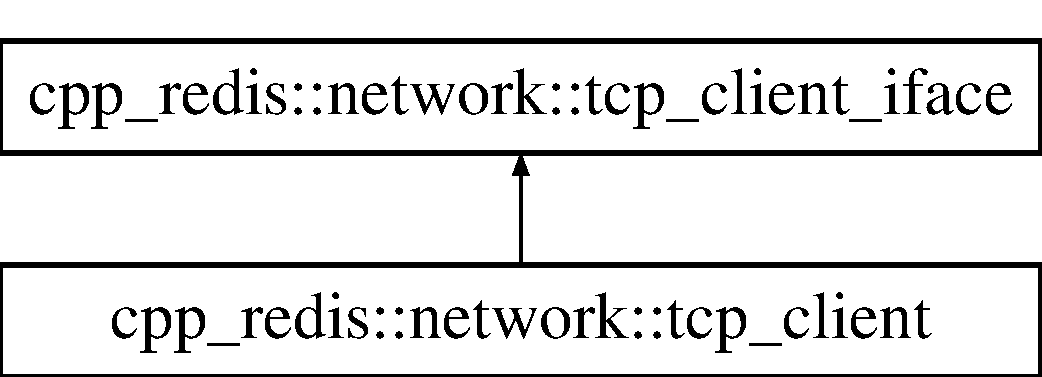
\includegraphics[height=2.000000cm]{classcpp__redis_1_1network_1_1tcp__client__iface}
\end{center}
\end{figure}
\subsection*{Classes}
\begin{DoxyCompactItemize}
\item 
struct \hyperlink{structcpp__redis_1_1network_1_1tcp__client__iface_1_1read__request}{read\+\_\+request}
\item 
struct \hyperlink{structcpp__redis_1_1network_1_1tcp__client__iface_1_1read__result}{read\+\_\+result}
\item 
struct \hyperlink{structcpp__redis_1_1network_1_1tcp__client__iface_1_1write__request}{write\+\_\+request}
\item 
struct \hyperlink{structcpp__redis_1_1network_1_1tcp__client__iface_1_1write__result}{write\+\_\+result}
\end{DoxyCompactItemize}
\subsection*{Public Types}
\begin{DoxyCompactItemize}
\item 
typedef std\+::function$<$ void(\hyperlink{structcpp__redis_1_1network_1_1tcp__client__iface_1_1read__result}{read\+\_\+result} \&)$>$ \hyperlink{classcpp__redis_1_1network_1_1tcp__client__iface_ae8bf79e8e1f1d7e359ed1c7cdc4026fc}{async\+\_\+read\+\_\+callback\+\_\+t}
\item 
typedef std\+::function$<$ void(\hyperlink{structcpp__redis_1_1network_1_1tcp__client__iface_1_1write__result}{write\+\_\+result} \&)$>$ \hyperlink{classcpp__redis_1_1network_1_1tcp__client__iface_a1dc52ccc70cf377c4fbb495a16adc658}{async\+\_\+write\+\_\+callback\+\_\+t}
\item 
typedef std\+::function$<$ void()$>$ \hyperlink{classcpp__redis_1_1network_1_1tcp__client__iface_a9a7d5942205db8be03da581a848b8ec0}{disconnection\+\_\+handler\+\_\+t}
\end{DoxyCompactItemize}
\subsection*{Public Member Functions}
\begin{DoxyCompactItemize}
\item 
\mbox{\Hypertarget{classcpp__redis_1_1network_1_1tcp__client__iface_a8504873049519bcebd626984e4087a90}\label{classcpp__redis_1_1network_1_1tcp__client__iface_a8504873049519bcebd626984e4087a90}} 
\hyperlink{classcpp__redis_1_1network_1_1tcp__client__iface_a8504873049519bcebd626984e4087a90}{tcp\+\_\+client\+\_\+iface} (void)=default
\begin{DoxyCompactList}\small\item\em ctor \end{DoxyCompactList}\item 
\mbox{\Hypertarget{classcpp__redis_1_1network_1_1tcp__client__iface_a7381e8921118a13b5994101864906122}\label{classcpp__redis_1_1network_1_1tcp__client__iface_a7381e8921118a13b5994101864906122}} 
virtual \hyperlink{classcpp__redis_1_1network_1_1tcp__client__iface_a7381e8921118a13b5994101864906122}{$\sim$tcp\+\_\+client\+\_\+iface} (void)=default
\begin{DoxyCompactList}\small\item\em dtor \end{DoxyCompactList}\item 
virtual void \hyperlink{classcpp__redis_1_1network_1_1tcp__client__iface_a81ee982136e85b7c3401393341bc594c}{connect} (const std\+::string \&addr, std\+::uint32\+\_\+t port, std\+::uint32\+\_\+t timeout\+\_\+msecs=0)=0
\item 
virtual void \hyperlink{classcpp__redis_1_1network_1_1tcp__client__iface_a024073fb3436d8fa99de8cad63418f6c}{disconnect} (bool wait\+\_\+for\+\_\+removal=false)=0
\item 
virtual bool \hyperlink{classcpp__redis_1_1network_1_1tcp__client__iface_a41ad0b43e3ab172828a3d2ce55d23893}{is\+\_\+connected} (void) const =0
\item 
virtual void \hyperlink{classcpp__redis_1_1network_1_1tcp__client__iface_ae1f9fa87002273a0caf340407bb68ade}{async\+\_\+read} (\hyperlink{structcpp__redis_1_1network_1_1tcp__client__iface_1_1read__request}{read\+\_\+request} \&request)=0
\item 
virtual void \hyperlink{classcpp__redis_1_1network_1_1tcp__client__iface_a9cd01e8a68479456d15d6435ffad9b92}{async\+\_\+write} (\hyperlink{structcpp__redis_1_1network_1_1tcp__client__iface_1_1write__request}{write\+\_\+request} \&request)=0
\item 
virtual void \hyperlink{classcpp__redis_1_1network_1_1tcp__client__iface_acecf3b75c3849071d82478bc7a8c97a8}{set\+\_\+on\+\_\+disconnection\+\_\+handler} (const \hyperlink{classcpp__redis_1_1network_1_1tcp__client__iface_a9a7d5942205db8be03da581a848b8ec0}{disconnection\+\_\+handler\+\_\+t} \&disconnection\+\_\+handler)=0
\end{DoxyCompactItemize}


\subsection{Detailed Description}
interface defining how tcp client should be implemented to be used inside cpp\+\_\+redis 

\subsection{Member Typedef Documentation}
\mbox{\Hypertarget{classcpp__redis_1_1network_1_1tcp__client__iface_ae8bf79e8e1f1d7e359ed1c7cdc4026fc}\label{classcpp__redis_1_1network_1_1tcp__client__iface_ae8bf79e8e1f1d7e359ed1c7cdc4026fc}} 
\index{cpp\+\_\+redis\+::network\+::tcp\+\_\+client\+\_\+iface@{cpp\+\_\+redis\+::network\+::tcp\+\_\+client\+\_\+iface}!async\+\_\+read\+\_\+callback\+\_\+t@{async\+\_\+read\+\_\+callback\+\_\+t}}
\index{async\+\_\+read\+\_\+callback\+\_\+t@{async\+\_\+read\+\_\+callback\+\_\+t}!cpp\+\_\+redis\+::network\+::tcp\+\_\+client\+\_\+iface@{cpp\+\_\+redis\+::network\+::tcp\+\_\+client\+\_\+iface}}
\subsubsection{\texorpdfstring{async\+\_\+read\+\_\+callback\+\_\+t}{async\_read\_callback\_t}}
{\footnotesize\ttfamily typedef std\+::function$<$void(\hyperlink{structcpp__redis_1_1network_1_1tcp__client__iface_1_1read__result}{read\+\_\+result}\&)$>$ \hyperlink{classcpp__redis_1_1network_1_1tcp__client__iface_ae8bf79e8e1f1d7e359ed1c7cdc4026fc}{cpp\+\_\+redis\+::network\+::tcp\+\_\+client\+\_\+iface\+::async\+\_\+read\+\_\+callback\+\_\+t}}

async read completion callbacks function taking \hyperlink{structcpp__redis_1_1network_1_1tcp__client__iface_1_1read__result}{read\+\_\+result} as a parameter \mbox{\Hypertarget{classcpp__redis_1_1network_1_1tcp__client__iface_a1dc52ccc70cf377c4fbb495a16adc658}\label{classcpp__redis_1_1network_1_1tcp__client__iface_a1dc52ccc70cf377c4fbb495a16adc658}} 
\index{cpp\+\_\+redis\+::network\+::tcp\+\_\+client\+\_\+iface@{cpp\+\_\+redis\+::network\+::tcp\+\_\+client\+\_\+iface}!async\+\_\+write\+\_\+callback\+\_\+t@{async\+\_\+write\+\_\+callback\+\_\+t}}
\index{async\+\_\+write\+\_\+callback\+\_\+t@{async\+\_\+write\+\_\+callback\+\_\+t}!cpp\+\_\+redis\+::network\+::tcp\+\_\+client\+\_\+iface@{cpp\+\_\+redis\+::network\+::tcp\+\_\+client\+\_\+iface}}
\subsubsection{\texorpdfstring{async\+\_\+write\+\_\+callback\+\_\+t}{async\_write\_callback\_t}}
{\footnotesize\ttfamily typedef std\+::function$<$void(\hyperlink{structcpp__redis_1_1network_1_1tcp__client__iface_1_1write__result}{write\+\_\+result}\&)$>$ \hyperlink{classcpp__redis_1_1network_1_1tcp__client__iface_a1dc52ccc70cf377c4fbb495a16adc658}{cpp\+\_\+redis\+::network\+::tcp\+\_\+client\+\_\+iface\+::async\+\_\+write\+\_\+callback\+\_\+t}}

async write completion callbacks function taking \hyperlink{structcpp__redis_1_1network_1_1tcp__client__iface_1_1write__result}{write\+\_\+result} as a parameter \mbox{\Hypertarget{classcpp__redis_1_1network_1_1tcp__client__iface_a9a7d5942205db8be03da581a848b8ec0}\label{classcpp__redis_1_1network_1_1tcp__client__iface_a9a7d5942205db8be03da581a848b8ec0}} 
\index{cpp\+\_\+redis\+::network\+::tcp\+\_\+client\+\_\+iface@{cpp\+\_\+redis\+::network\+::tcp\+\_\+client\+\_\+iface}!disconnection\+\_\+handler\+\_\+t@{disconnection\+\_\+handler\+\_\+t}}
\index{disconnection\+\_\+handler\+\_\+t@{disconnection\+\_\+handler\+\_\+t}!cpp\+\_\+redis\+::network\+::tcp\+\_\+client\+\_\+iface@{cpp\+\_\+redis\+::network\+::tcp\+\_\+client\+\_\+iface}}
\subsubsection{\texorpdfstring{disconnection\+\_\+handler\+\_\+t}{disconnection\_handler\_t}}
{\footnotesize\ttfamily typedef std\+::function$<$void()$>$ \hyperlink{classcpp__redis_1_1network_1_1tcp__client__iface_a9a7d5942205db8be03da581a848b8ec0}{cpp\+\_\+redis\+::network\+::tcp\+\_\+client\+\_\+iface\+::disconnection\+\_\+handler\+\_\+t}}

disconnection handler 

\subsection{Member Function Documentation}
\mbox{\Hypertarget{classcpp__redis_1_1network_1_1tcp__client__iface_ae1f9fa87002273a0caf340407bb68ade}\label{classcpp__redis_1_1network_1_1tcp__client__iface_ae1f9fa87002273a0caf340407bb68ade}} 
\index{cpp\+\_\+redis\+::network\+::tcp\+\_\+client\+\_\+iface@{cpp\+\_\+redis\+::network\+::tcp\+\_\+client\+\_\+iface}!async\+\_\+read@{async\+\_\+read}}
\index{async\+\_\+read@{async\+\_\+read}!cpp\+\_\+redis\+::network\+::tcp\+\_\+client\+\_\+iface@{cpp\+\_\+redis\+::network\+::tcp\+\_\+client\+\_\+iface}}
\subsubsection{\texorpdfstring{async\+\_\+read()}{async\_read()}}
{\footnotesize\ttfamily virtual void cpp\+\_\+redis\+::network\+::tcp\+\_\+client\+\_\+iface\+::async\+\_\+read (\begin{DoxyParamCaption}\item[{\hyperlink{structcpp__redis_1_1network_1_1tcp__client__iface_1_1read__request}{read\+\_\+request} \&}]{request }\end{DoxyParamCaption})\hspace{0.3cm}{\ttfamily [pure virtual]}}

async read operation


\begin{DoxyParams}{Parameters}
{\em request} & information about what should be read and what should be done after completion \\
\hline
\end{DoxyParams}


Implemented in \hyperlink{classcpp__redis_1_1network_1_1tcp__client_a5eed4225fcd01e3108580d863c94c2cc}{cpp\+\_\+redis\+::network\+::tcp\+\_\+client}.

\mbox{\Hypertarget{classcpp__redis_1_1network_1_1tcp__client__iface_a9cd01e8a68479456d15d6435ffad9b92}\label{classcpp__redis_1_1network_1_1tcp__client__iface_a9cd01e8a68479456d15d6435ffad9b92}} 
\index{cpp\+\_\+redis\+::network\+::tcp\+\_\+client\+\_\+iface@{cpp\+\_\+redis\+::network\+::tcp\+\_\+client\+\_\+iface}!async\+\_\+write@{async\+\_\+write}}
\index{async\+\_\+write@{async\+\_\+write}!cpp\+\_\+redis\+::network\+::tcp\+\_\+client\+\_\+iface@{cpp\+\_\+redis\+::network\+::tcp\+\_\+client\+\_\+iface}}
\subsubsection{\texorpdfstring{async\+\_\+write()}{async\_write()}}
{\footnotesize\ttfamily virtual void cpp\+\_\+redis\+::network\+::tcp\+\_\+client\+\_\+iface\+::async\+\_\+write (\begin{DoxyParamCaption}\item[{\hyperlink{structcpp__redis_1_1network_1_1tcp__client__iface_1_1write__request}{write\+\_\+request} \&}]{request }\end{DoxyParamCaption})\hspace{0.3cm}{\ttfamily [pure virtual]}}

async write operation


\begin{DoxyParams}{Parameters}
{\em request} & information about what should be written and what should be done after completion \\
\hline
\end{DoxyParams}


Implemented in \hyperlink{classcpp__redis_1_1network_1_1tcp__client_a6d15785b71776cd85426c9634cb446f0}{cpp\+\_\+redis\+::network\+::tcp\+\_\+client}.

\mbox{\Hypertarget{classcpp__redis_1_1network_1_1tcp__client__iface_a81ee982136e85b7c3401393341bc594c}\label{classcpp__redis_1_1network_1_1tcp__client__iface_a81ee982136e85b7c3401393341bc594c}} 
\index{cpp\+\_\+redis\+::network\+::tcp\+\_\+client\+\_\+iface@{cpp\+\_\+redis\+::network\+::tcp\+\_\+client\+\_\+iface}!connect@{connect}}
\index{connect@{connect}!cpp\+\_\+redis\+::network\+::tcp\+\_\+client\+\_\+iface@{cpp\+\_\+redis\+::network\+::tcp\+\_\+client\+\_\+iface}}
\subsubsection{\texorpdfstring{connect()}{connect()}}
{\footnotesize\ttfamily virtual void cpp\+\_\+redis\+::network\+::tcp\+\_\+client\+\_\+iface\+::connect (\begin{DoxyParamCaption}\item[{const std\+::string \&}]{addr,  }\item[{std\+::uint32\+\_\+t}]{port,  }\item[{std\+::uint32\+\_\+t}]{timeout\+\_\+msecs = {\ttfamily 0} }\end{DoxyParamCaption})\hspace{0.3cm}{\ttfamily [pure virtual]}}

start the tcp client


\begin{DoxyParams}{Parameters}
{\em addr} & host to be connected to \\
\hline
{\em port} & port to be connected to \\
\hline
{\em timeout\+\_\+msecs} & max time to connect in ms \\
\hline
\end{DoxyParams}


Implemented in \hyperlink{classcpp__redis_1_1network_1_1tcp__client_a5808c0569980d83479f755ac55a12dfb}{cpp\+\_\+redis\+::network\+::tcp\+\_\+client}.

\mbox{\Hypertarget{classcpp__redis_1_1network_1_1tcp__client__iface_a024073fb3436d8fa99de8cad63418f6c}\label{classcpp__redis_1_1network_1_1tcp__client__iface_a024073fb3436d8fa99de8cad63418f6c}} 
\index{cpp\+\_\+redis\+::network\+::tcp\+\_\+client\+\_\+iface@{cpp\+\_\+redis\+::network\+::tcp\+\_\+client\+\_\+iface}!disconnect@{disconnect}}
\index{disconnect@{disconnect}!cpp\+\_\+redis\+::network\+::tcp\+\_\+client\+\_\+iface@{cpp\+\_\+redis\+::network\+::tcp\+\_\+client\+\_\+iface}}
\subsubsection{\texorpdfstring{disconnect()}{disconnect()}}
{\footnotesize\ttfamily virtual void cpp\+\_\+redis\+::network\+::tcp\+\_\+client\+\_\+iface\+::disconnect (\begin{DoxyParamCaption}\item[{bool}]{wait\+\_\+for\+\_\+removal = {\ttfamily false} }\end{DoxyParamCaption})\hspace{0.3cm}{\ttfamily [pure virtual]}}

stop the tcp client


\begin{DoxyParams}{Parameters}
{\em wait\+\_\+for\+\_\+removal} & when sets to true, disconnect blocks until the underlying T\+CP client has been effectively removed from the io\+\_\+service and that all the underlying callbacks have completed. \\
\hline
\end{DoxyParams}


Implemented in \hyperlink{classcpp__redis_1_1network_1_1tcp__client_a88f49c4e32d59855a62296fb74136a44}{cpp\+\_\+redis\+::network\+::tcp\+\_\+client}.

\mbox{\Hypertarget{classcpp__redis_1_1network_1_1tcp__client__iface_a41ad0b43e3ab172828a3d2ce55d23893}\label{classcpp__redis_1_1network_1_1tcp__client__iface_a41ad0b43e3ab172828a3d2ce55d23893}} 
\index{cpp\+\_\+redis\+::network\+::tcp\+\_\+client\+\_\+iface@{cpp\+\_\+redis\+::network\+::tcp\+\_\+client\+\_\+iface}!is\+\_\+connected@{is\+\_\+connected}}
\index{is\+\_\+connected@{is\+\_\+connected}!cpp\+\_\+redis\+::network\+::tcp\+\_\+client\+\_\+iface@{cpp\+\_\+redis\+::network\+::tcp\+\_\+client\+\_\+iface}}
\subsubsection{\texorpdfstring{is\+\_\+connected()}{is\_connected()}}
{\footnotesize\ttfamily virtual bool cpp\+\_\+redis\+::network\+::tcp\+\_\+client\+\_\+iface\+::is\+\_\+connected (\begin{DoxyParamCaption}\item[{void}]{ }\end{DoxyParamCaption}) const\hspace{0.3cm}{\ttfamily [pure virtual]}}

\begin{DoxyReturn}{Returns}
whether the client is currently connected or not 
\end{DoxyReturn}


Implemented in \hyperlink{classcpp__redis_1_1network_1_1tcp__client_a0a636ca6bd59425bf22416a1c7694f65}{cpp\+\_\+redis\+::network\+::tcp\+\_\+client}.

\mbox{\Hypertarget{classcpp__redis_1_1network_1_1tcp__client__iface_acecf3b75c3849071d82478bc7a8c97a8}\label{classcpp__redis_1_1network_1_1tcp__client__iface_acecf3b75c3849071d82478bc7a8c97a8}} 
\index{cpp\+\_\+redis\+::network\+::tcp\+\_\+client\+\_\+iface@{cpp\+\_\+redis\+::network\+::tcp\+\_\+client\+\_\+iface}!set\+\_\+on\+\_\+disconnection\+\_\+handler@{set\+\_\+on\+\_\+disconnection\+\_\+handler}}
\index{set\+\_\+on\+\_\+disconnection\+\_\+handler@{set\+\_\+on\+\_\+disconnection\+\_\+handler}!cpp\+\_\+redis\+::network\+::tcp\+\_\+client\+\_\+iface@{cpp\+\_\+redis\+::network\+::tcp\+\_\+client\+\_\+iface}}
\subsubsection{\texorpdfstring{set\+\_\+on\+\_\+disconnection\+\_\+handler()}{set\_on\_disconnection\_handler()}}
{\footnotesize\ttfamily virtual void cpp\+\_\+redis\+::network\+::tcp\+\_\+client\+\_\+iface\+::set\+\_\+on\+\_\+disconnection\+\_\+handler (\begin{DoxyParamCaption}\item[{const \hyperlink{classcpp__redis_1_1network_1_1tcp__client__iface_a9a7d5942205db8be03da581a848b8ec0}{disconnection\+\_\+handler\+\_\+t} \&}]{disconnection\+\_\+handler }\end{DoxyParamCaption})\hspace{0.3cm}{\ttfamily [pure virtual]}}

set on disconnection handler


\begin{DoxyParams}{Parameters}
{\em disconnection\+\_\+handler} & handler to be called in case of a disconnection \\
\hline
\end{DoxyParams}


Implemented in \hyperlink{classcpp__redis_1_1network_1_1tcp__client_a24ccdf6dc467aac13cb832a395adb38d}{cpp\+\_\+redis\+::network\+::tcp\+\_\+client}.



The documentation for this class was generated from the following file\+:\begin{DoxyCompactItemize}
\item 
includes/cpp\+\_\+redis/network/tcp\+\_\+client\+\_\+iface.\+hpp\end{DoxyCompactItemize}

\hypertarget{structcpp__redis_1_1network_1_1tcp__client__iface_1_1write__request}{}\section{cpp\+\_\+redis\+:\+:network\+:\+:tcp\+\_\+client\+\_\+iface\+:\+:write\+\_\+request Struct Reference}
\label{structcpp__redis_1_1network_1_1tcp__client__iface_1_1write__request}\index{cpp\+\_\+redis\+::network\+::tcp\+\_\+client\+\_\+iface\+::write\+\_\+request@{cpp\+\_\+redis\+::network\+::tcp\+\_\+client\+\_\+iface\+::write\+\_\+request}}


{\ttfamily \#include $<$tcp\+\_\+client\+\_\+iface.\+hpp$>$}

\subsection*{Public Attributes}
\begin{DoxyCompactItemize}
\item 
std\+::vector$<$ char $>$ \hyperlink{structcpp__redis_1_1network_1_1tcp__client__iface_1_1write__request_ad3567dac827f550b60491af530f0db2e}{buffer}
\item 
\hyperlink{classcpp__redis_1_1network_1_1tcp__client__iface_a1dc52ccc70cf377c4fbb495a16adc658}{async\+\_\+write\+\_\+callback\+\_\+t} \hyperlink{structcpp__redis_1_1network_1_1tcp__client__iface_1_1write__request_ab2823d9836ec68d63c9799ee12d403a2}{async\+\_\+write\+\_\+callback}
\end{DoxyCompactItemize}


\subsection{Detailed Description}
structure to store write requests information 

\subsection{Member Data Documentation}
\mbox{\Hypertarget{structcpp__redis_1_1network_1_1tcp__client__iface_1_1write__request_ab2823d9836ec68d63c9799ee12d403a2}\label{structcpp__redis_1_1network_1_1tcp__client__iface_1_1write__request_ab2823d9836ec68d63c9799ee12d403a2}} 
\index{cpp\+\_\+redis\+::network\+::tcp\+\_\+client\+\_\+iface\+::write\+\_\+request@{cpp\+\_\+redis\+::network\+::tcp\+\_\+client\+\_\+iface\+::write\+\_\+request}!async\+\_\+write\+\_\+callback@{async\+\_\+write\+\_\+callback}}
\index{async\+\_\+write\+\_\+callback@{async\+\_\+write\+\_\+callback}!cpp\+\_\+redis\+::network\+::tcp\+\_\+client\+\_\+iface\+::write\+\_\+request@{cpp\+\_\+redis\+::network\+::tcp\+\_\+client\+\_\+iface\+::write\+\_\+request}}
\subsubsection{\texorpdfstring{async\+\_\+write\+\_\+callback}{async\_write\_callback}}
{\footnotesize\ttfamily \hyperlink{classcpp__redis_1_1network_1_1tcp__client__iface_a1dc52ccc70cf377c4fbb495a16adc658}{async\+\_\+write\+\_\+callback\+\_\+t} cpp\+\_\+redis\+::network\+::tcp\+\_\+client\+\_\+iface\+::write\+\_\+request\+::async\+\_\+write\+\_\+callback}

\mbox{\Hypertarget{structcpp__redis_1_1network_1_1tcp__client__iface_1_1write__request_ad3567dac827f550b60491af530f0db2e}\label{structcpp__redis_1_1network_1_1tcp__client__iface_1_1write__request_ad3567dac827f550b60491af530f0db2e}} 
\index{cpp\+\_\+redis\+::network\+::tcp\+\_\+client\+\_\+iface\+::write\+\_\+request@{cpp\+\_\+redis\+::network\+::tcp\+\_\+client\+\_\+iface\+::write\+\_\+request}!buffer@{buffer}}
\index{buffer@{buffer}!cpp\+\_\+redis\+::network\+::tcp\+\_\+client\+\_\+iface\+::write\+\_\+request@{cpp\+\_\+redis\+::network\+::tcp\+\_\+client\+\_\+iface\+::write\+\_\+request}}
\subsubsection{\texorpdfstring{buffer}{buffer}}
{\footnotesize\ttfamily std\+::vector$<$char$>$ cpp\+\_\+redis\+::network\+::tcp\+\_\+client\+\_\+iface\+::write\+\_\+request\+::buffer}



The documentation for this struct was generated from the following file\+:\begin{DoxyCompactItemize}
\item 
includes/cpp\+\_\+redis/network/\hyperlink{tcp__client__iface_8hpp}{tcp\+\_\+client\+\_\+iface.\+hpp}\end{DoxyCompactItemize}

\hypertarget{structcpp__redis_1_1network_1_1tcp__client__iface_1_1write__result}{}\section{cpp\+\_\+redis\+:\+:network\+:\+:tcp\+\_\+client\+\_\+iface\+:\+:write\+\_\+result Struct Reference}
\label{structcpp__redis_1_1network_1_1tcp__client__iface_1_1write__result}\index{cpp\+\_\+redis\+::network\+::tcp\+\_\+client\+\_\+iface\+::write\+\_\+result@{cpp\+\_\+redis\+::network\+::tcp\+\_\+client\+\_\+iface\+::write\+\_\+result}}


{\ttfamily \#include $<$tcp\+\_\+client\+\_\+iface.\+hpp$>$}

\subsection*{Public Attributes}
\begin{DoxyCompactItemize}
\item 
bool \hyperlink{structcpp__redis_1_1network_1_1tcp__client__iface_1_1write__result_a677696941c9a7164bc0b93b5d8380d1a}{success}
\item 
std\+::size\+\_\+t \hyperlink{structcpp__redis_1_1network_1_1tcp__client__iface_1_1write__result_a580f3dbe5ea3f6f4b6b4ca0bfad2c06c}{size}
\end{DoxyCompactItemize}


\subsection{Detailed Description}
structure to store write requests result 

\subsection{Member Data Documentation}
\mbox{\Hypertarget{structcpp__redis_1_1network_1_1tcp__client__iface_1_1write__result_a580f3dbe5ea3f6f4b6b4ca0bfad2c06c}\label{structcpp__redis_1_1network_1_1tcp__client__iface_1_1write__result_a580f3dbe5ea3f6f4b6b4ca0bfad2c06c}} 
\index{cpp\+\_\+redis\+::network\+::tcp\+\_\+client\+\_\+iface\+::write\+\_\+result@{cpp\+\_\+redis\+::network\+::tcp\+\_\+client\+\_\+iface\+::write\+\_\+result}!size@{size}}
\index{size@{size}!cpp\+\_\+redis\+::network\+::tcp\+\_\+client\+\_\+iface\+::write\+\_\+result@{cpp\+\_\+redis\+::network\+::tcp\+\_\+client\+\_\+iface\+::write\+\_\+result}}
\subsubsection{\texorpdfstring{size}{size}}
{\footnotesize\ttfamily std\+::size\+\_\+t cpp\+\_\+redis\+::network\+::tcp\+\_\+client\+\_\+iface\+::write\+\_\+result\+::size}

number of bytes written \mbox{\Hypertarget{structcpp__redis_1_1network_1_1tcp__client__iface_1_1write__result_a677696941c9a7164bc0b93b5d8380d1a}\label{structcpp__redis_1_1network_1_1tcp__client__iface_1_1write__result_a677696941c9a7164bc0b93b5d8380d1a}} 
\index{cpp\+\_\+redis\+::network\+::tcp\+\_\+client\+\_\+iface\+::write\+\_\+result@{cpp\+\_\+redis\+::network\+::tcp\+\_\+client\+\_\+iface\+::write\+\_\+result}!success@{success}}
\index{success@{success}!cpp\+\_\+redis\+::network\+::tcp\+\_\+client\+\_\+iface\+::write\+\_\+result@{cpp\+\_\+redis\+::network\+::tcp\+\_\+client\+\_\+iface\+::write\+\_\+result}}
\subsubsection{\texorpdfstring{success}{success}}
{\footnotesize\ttfamily bool cpp\+\_\+redis\+::network\+::tcp\+\_\+client\+\_\+iface\+::write\+\_\+result\+::success}

whether the operation succeeded or not 

The documentation for this struct was generated from the following file\+:\begin{DoxyCompactItemize}
\item 
includes/cpp\+\_\+redis/network/tcp\+\_\+client\+\_\+iface.\+hpp\end{DoxyCompactItemize}

%--- End generated contents ---

% Index
\backmatter
\newpage
\phantomsection
\clearemptydoublepage
\addcontentsline{toc}{chapter}{Index}
\printindex

\end{document}
